\documentclass[11pt,openany]{book}

% --- Page geometry ---
\usepackage[margin=1in,marginparwidth=0.8in]{geometry}

% --- Fonts and encoding ---
\usepackage[T1]{fontenc}
\usepackage{lmodern}
\usepackage{microtype}

% --- Math ---
\usepackage{amsmath,amssymb,amsfonts}

% --- Graphics and figures ---
\usepackage{tikz}
\usetikzlibrary{arrows.meta,positioning,shapes.geometric,calc,decorations.pathreplacing,patterns}
\usepackage{graphicx}

% --- Colors ---
\usepackage{xcolor}
\definecolor{noteblue}{RGB}{30,50,100}
\definecolor{insightgreen}{RGB}{0,100,50}
\definecolor{bugred}{RGB}{150,30,30}

% --- Colored boxes ---
\usepackage[most]{tcolorbox}
\newtcolorbox{notebox}{
  colback=blue!5!white,
  colframe=noteblue,
  fonttitle=\bfseries\ttfamily,
  title=Note,
  sharp corners,
  boxrule=0.8pt,
  left=6pt,right=6pt,top=4pt,bottom=4pt
}

\newtcolorbox{insightbox}{
  colback=green!5!white,
  colframe=insightgreen,
  fonttitle=\bfseries,
  title=Key Insight,
  sharp corners,
  boxrule=0.8pt,
  left=6pt,right=6pt,top=4pt,bottom=4pt
}

\newtcolorbox{bugbox}{
  colback=red!5!white,
  colframe=bugred,
  fonttitle=\bfseries,
  title=Bug,
  sharp corners,
  boxrule=0.8pt,
  left=6pt,right=6pt,top=4pt,bottom=4pt
}

\definecolor{whynotbrown}{RGB}{140,90,20}
\newtcolorbox{whynotbox}[1]{
  colback=orange!5!white,
  colframe=whynotbrown,
  fonttitle=\bfseries,
  title=#1,
  sharp corners,
  boxrule=0.8pt,
  left=6pt,right=6pt,top=4pt,bottom=4pt
}

% --- Margin notes ---
\usepackage{marginnote}
\renewcommand*{\marginfont}{\footnotesize\itshape}

% --- Code ---
\usepackage{listings}
\lstdefinelanguage{Rust}{
  keywords={fn, let, mut, pub, struct, enum, impl, use, mod, self, super, crate, trait, type, where, as, in, for, loop, while, if, else, match, return, break, continue, move, ref, static, const, unsafe, extern, async, await, dyn, true, false, Some, None, Ok, Err, Vec, String, Box, Rc, Arc, RefCell, HashMap, FxHashMap, u8, u16, u32, u64, usize, i8, i16, i32, i64, isize, f32, f64, bool, str, Self},
  comment=[l]{//},
  morecomment=[s]{/*}{*/},
  morestring=[b]",
  sensitive=true,
}
\lstset{
  basicstyle=\ttfamily\small,
  breaklines=true,
  frame=none,
  columns=flexible,
  keepspaces=true
}

% --- Hyperlinks ---
\usepackage{hyperref}
\hypersetup{
  colorlinks=true,
  linkcolor=blue!60!black,
  citecolor=blue!60!black,
  urlcolor=blue!60!black
}

% --- Headers ---
\usepackage{fancyhdr}
\setlength{\headheight}{14pt}
\pagestyle{fancy}
\fancyhf{}
\fancyhead[LE]{\thepage\hspace{2em}\nouppercase{\leftmark}}
\fancyhead[RO]{\nouppercase{\rightmark}\hspace{2em}\thepage}
\renewcommand{\headrulewidth}{0.4pt}

% --- Chapter style ---
\usepackage{titlesec}

% --- Enumerate/itemize ---
\usepackage{enumitem}

% --- Algorithms ---
\usepackage{algorithm}
\usepackage{algpseudocode}

% --- Tables ---
\usepackage{booktabs}

% --- For underbrace labels ---
\usepackage{mathtools}

\begin{document}

\chapter{Introduction}

\section{What Happens When You Hit Send}

You type a message into a chat interface and press \emph{Send}. An HTTP request leaves your browser, carrying a JSON payload with your prompt. A \emph{frontend server} receives it and hands it to a \emph{preprocessor}, which applies a chat template and feeds your text through a \emph{tokenizer}---an algorithm that splits your text into integer-coded sub-word pieces called \emph{tokens}. The resulting sequence of token IDs is forwarded to a \emph{router}, which hashes them into fixed-size blocks and queries a \emph{radix tree}---a prefix data structure that maps block hashes to cached GPU workers. The router selects the GPU whose memory already contains the most relevant cached computation from prior requests. A custom \emph{binary codec} serializes the token sequence and ships it over TCP to the chosen GPU worker. There, an inference engine streams the model's billions of already-resident parameters from high-bandwidth memory, runs the \emph{transformer}'s attention mechanism against the input, and produces a single new token. That token streams back through the system as a Server-Sent Event. The process repeats---one token at a time---until the model emits a stop signal.

Every italicized term above is a promise. Over the next nine chapters, we will explain each one from scratch, building from the linear algebra inside a single GPU all the way out to the distributed system that orchestrates hundreds of them.


\section{What Dynamo Is}

NVIDIA Dynamo is an open-source, distributed inference-serving framework designed to orchestrate large language model (LLM) inference across multi-node GPU clusters. Built primarily in Rust, with Go for deployment infrastructure (Kubernetes operator, API server), and Python for extensibility, it represents a new class of infrastructure software: \emph{AI serving infrastructure}---systems that sit between users and AI models, managing GPU memory, network communication, and request routing to make real-time AI possible at scale.

Dynamo implements several techniques drawn from recent systems research:
\begin{itemize}
  \item \textbf{KV-cache-aware routing}: A radix tree tracks which key-value cache blocks are stored on which GPUs, enabling the router to maximize cache reuse and avoid redundant computation.
  \item \textbf{Disaggregated serving}: Prefill (compute-heavy prompt processing) and decode (memory-heavy token generation) run on separate, independently scaled GPU pools.
  \item \textbf{Continuous batching}: Requests enter and exit the GPU's processing batch at the granularity of individual iterations rather than waiting for a full batch to complete.
  \item \textbf{Custom binary protocols}: A zero-copy TCP codec handles all inter-service communication with a 24-byte fixed preamble followed by variable-length header and body payloads.
\end{itemize}


\section{The Language: Why Rust}

Dynamo's performance-critical infrastructure---the binary codec, the radix tree, the router, the frontend HTTP server---is written in Rust.\footnote{Rust comprises roughly 55\% of the Dynamo codebase by lines of code, with Python at $\sim$27\% and Go at $\sim$12\%.} This is not incidental. Rust was designed for exactly this class of problem: high-throughput, low-latency network services where both performance and correctness are non-negotiable.

\begin{notebox}
If you are not familiar with Rust, you can safely skim this section on first reading. The concepts introduced here---ownership, \texttt{RefCell}, traits---will be revisited in context when they appear in later chapters. The key takeaway is that Rust provides memory safety and high performance without garbage collection, which is essential for a latency-sensitive system like Dynamo.
\end{notebox}

\subsection{Why Rust for Inference Serving}

Three properties make Rust particularly well-suited to inference infrastructure:

\textbf{Memory safety without a garbage collector.}\hspace{1em} Inference serving must deliver tokens with consistent, low tail latency. A garbage-collected runtime (Java, Go) introduces unpredictable pauses: the GC can halt all threads for milliseconds while it reclaims memory. Python avoids stop-the-world collection through reference counting, but still incurs non-deterministic overhead from cycle collection and the global interpreter lock. At Dynamo's throughput targets---thousands of concurrent requests, each generating tokens every few milliseconds---even a brief GC pause cascades into visible user-facing latency spikes. Discord famously migrated its Read States service from Go to Rust precisely to eliminate such spikes. Rust's \emph{ownership system} guarantees memory safety at \emph{compile time}, with zero runtime overhead: no GC pauses, no reference counting on the hot path, no stop-the-world collection.

\textbf{Fearless concurrency.}\hspace{1em} Dynamo orchestrates hundreds of GPU workers with concurrent requests flowing through routers, codecs, and parsers. Rust's ownership system extends to concurrency: the compiler prevents \emph{data races at compile time}. If two threads need shared access to data, the type system forces the use of synchronization primitives (\texttt{Mutex}, \texttt{RwLock}, \texttt{Arc}). Code that accidentally shares mutable state across threads simply will not compile. For a serving system where a data race in routing logic could silently misroute requests to the wrong GPU, this compile-time guarantee is invaluable.

\textbf{C/C++-class performance.}\hspace{1em} Rust uses the same LLVM backend as Clang and achieves performance within single-digit percentage points of C++ on computational workloads. It achieves this through \emph{zero-cost abstractions}: iterators, closures, and generics all compile to the same machine code as hand-written loops and specialized functions. The principle, borrowed from C++, is: ``What you don't use, you don't pay for. What you do use, you couldn't hand-code any better.'' For Dynamo, this means the \texttt{TwoPartCodec} that decodes every inter-service TCP message runs at the speed of hand-tuned C, but with memory safety guaranteed by the compiler.

\begin{notebox}
Rust's adoption in performance-critical infrastructure is well-established. AWS Firecracker (which powers Lambda) is written in Rust and starts microVMs in under 125\,ms. Cloudflare's Pingora, a Rust rewrite of their NGINX-based proxy, serves over a trillion requests daily with 70\% less CPU and 67\% less memory than the NGINX-based system it replaced. In the AI ecosystem specifically, Hugging Face Tokenizers (Rust core, Python bindings) achieves a 43$\times$ speedup over its pure-Python predecessor.
\end{notebox}


\subsection{Rust Concepts for This Guide}

The remaining chapters reference several Rust-specific concepts. We introduce them briefly here; each will be revisited in context when it appears.

\textbf{Ownership and borrowing.}\hspace{1em} Every value in Rust has exactly one \emph{owner}. When the owner goes out of scope, the value is freed---no garbage collector involved. You can create \emph{references} (borrows) to a value without taking ownership, subject to one rule: you may have either any number of immutable references (\texttt{\&T}) or exactly one mutable reference (\texttt{\&mut T}), but never both simultaneously. The borrow checker enforces this at compile time, preventing dangling pointers and data races with zero runtime cost.

\textbf{Enums and pattern matching.}\hspace{1em} Rust's enums are \emph{algebraic data types}: each variant can carry associated data. The two most important are \texttt{Option<T>} (\texttt{Some(T)} or \texttt{None}, replacing null pointers) and \texttt{Result<T, E>} (\texttt{Ok(T)} or \texttt{Err(E)}, for recoverable errors). The compiler enforces \emph{exhaustive matching}: every variant must be handled. This is pervasive in Dynamo---parsers return \texttt{Result} types, codec decoders return \texttt{Result<Option<...>{}>}, and the \texttt{match} statement dispatches across parser configurations (Chapter~\ref{ch:codecs}).

\textbf{Error handling and panics.}\hspace{1em} Rust has no exceptions. Recoverable errors use \texttt{Result}; the \texttt{?} operator propagates errors concisely. \emph{Unrecoverable} errors trigger a \textbf{panic}: the thread aborts with a backtrace. Panics arise from integer overflow (in debug builds), out-of-bounds indexing, calling \texttt{.unwrap()} on \texttt{None} or \texttt{Err}, division by zero, and explicit \texttt{panic!()} calls. In a server, a panic in a request handler kills the task---or the entire service. Every crash bug in Chapter~\ref{ch:findings} is a panic.

\textbf{Interior mutability.}\hspace{1em} Sometimes you need to mutate data through a shared reference---for instance, updating a data structure node reachable through multiple reference-counted pointers. Rust provides \texttt{RefCell<T>}\footnote{\texttt{Rc<RefCell<T>{}>} provides shared ownership (\texttt{Rc}) with interior mutability (\texttt{RefCell}). The thread-safe equivalent is \texttt{Arc<RwLock<T>{}>}.}, which moves the borrow check from compile time to runtime: \texttt{.borrow()} for shared access, \texttt{.borrow\_mut()} for exclusive access. If the borrowing rules are violated at runtime---for example, taking two mutable borrows on the same cell---\texttt{RefCell} \emph{panics}. This is exactly how Bug~16 (Chapter~\ref{ch:findings}) manifests: the radix tree uses \texttt{Rc<RefCell<RadixBlock>{}>}, and when a node becomes its own child due to hash collisions, a mutable borrow on the parent followed by an immutable borrow on the child panics because they are the same \texttt{RefCell}.

\textbf{Traits.}\hspace{1em} Rust's mechanism for polymorphism. A trait defines a set of methods that types must implement---similar to interfaces in other languages. Dynamo's reasoning parsers all implement a single \texttt{ReasoningParser} trait (Chapter~\ref{ch:codecs}), allowing the system to dispatch to any of eleven parser variants through a uniform interface.


\subsection{What Rust Does and Does Not Prevent}

This distinction is fundamental to the fuzzing campaign in Chapters~\ref{ch:fuzzing}--\ref{ch:findings}:
\begin{itemize}
  \item \textbf{Rust prevents}: buffer overflows, use-after-free, double-free, dangling pointers, data races, and null pointer dereferences. These are enforced by the compiler in safe code. The traditional targets of memory-corruption fuzzing largely do not exist.
  \item \textbf{Rust does not prevent}: panics (denial-of-service bugs), logic errors (silent data corruption), \texttt{RefCell} violations (runtime borrow-check panics), or \texttt{Mutex} misuse (deadlocks). These are the bugs our campaign found.
\end{itemize}

There is one additional subtlety: \textbf{debug vs.\ release divergence}. Rust compiles with integer overflow checks in debug mode (overflow panics) and without them in release mode (overflow wraps silently via two's complement). The same code can crash in debug and produce silently wrong results in release. Bug~18---the critical integer overflow in the network codec (Chapter~\ref{ch:findings})---exploits exactly this divergence.


\subsection{The Rust--Python Bridge}

\marginnote{\emph{PyO3 generates Python extension modules from Rust code. The build tool Maturin compiles Rust into Python wheels.}}%
Dynamo is not a pure Rust system. The GPU inference engines it orchestrates---vLLM, SGLang, TensorRT-LLM---are all Python-first. Model configuration, custom preprocessing, and operator-facing APIs are written in Python. The bridge between the two languages is \textbf{PyO3}, a Rust library that enables bidirectional function calls between Rust and Python with near-zero overhead.

The architectural split is deliberate: Rust handles the \emph{hot path}---network I/O, binary protocol encoding/decoding, data structure operations, request routing---where microsecond latency matters. Python handles the \emph{configuration path}---model loading, inference engine integration, scaling policies---where flexibility matters more than raw speed. This pattern is increasingly common in AI infrastructure: Hugging Face Tokenizers (Rust core, Python API), Polars (Rust DataFrame library with Python bindings), and Pydantic v2 (Rust validation core, 4--50$\times$ faster than the pure-Python v1) all follow the same design.


\section{Dynamo in Context: The Inference Runtime Landscape}

Dynamo does not exist in a vacuum. It enters a crowded field of LLM inference runtimes, each approaching the same fundamental problem---serving transformer models fast and efficiently---from a different angle. Understanding where Dynamo sits in this landscape explains both why it exists and why studying it teaches generalizable lessons about the entire category.

\textbf{vLLM}\hspace{1em} is the most widely adopted open-source inference engine. Developed at UC Berkeley, it introduced \textbf{PagedAttention}---the technique that revolutionized KV cache memory management by applying OS-style virtual memory paging to GPU memory (Chapter~\ref{ch:kvcache}). vLLM handles batching, scheduling, and memory management, and can span multiple nodes for tensor and pipeline parallelism. What it does not do, by itself, is manage a \emph{fleet} of independent model replicas across a cluster---routing requests based on cache state, coordinating prefill and decode across separate GPU pools, or performing KV cache transfers between disaggregated workers.

\textbf{SGLang}\hspace{1em} (from LMSYS, a collaboration spanning UC Berkeley, CMU, and others) takes a programming-language approach to LLM serving. Its key contribution is \textbf{RadixAttention}---a radix tree that tracks cached KV blocks at the \emph{token level} to enable prefix sharing across requests. This is the same core idea behind Dynamo's KV-aware routing (Chapter~\ref{ch:kvrouter}), though Dynamo operates at \emph{block granularity} rather than individual tokens, trades some precision for lower overhead, and extends the concept into a fleet-level orchestration layer. SGLang also supports multi-GPU and multi-node serving with distributed RadixAttention, and its Cache-Aware Load Balancer shares DNA with Dynamo's routing logic.

\textbf{TensorRT-LLM}\hspace{1em} is NVIDIA's own high-performance inference library, optimized for NVIDIA GPUs at the kernel level. It provides the fastest raw inference throughput through custom CUDA kernels, quantization support, and hardware-specific optimizations. Like vLLM, it supports multi-node tensor and pipeline parallelism via NCCL, but its focus is on maximizing single-model throughput rather than fleet-level orchestration.

\textbf{Where Dynamo fits.}\hspace{1em} The critical distinction is between an \emph{inference engine} and an \emph{inference orchestrator}. vLLM, SGLang, and TensorRT-LLM are engines: they execute model inference on GPUs and can scale a single model across nodes. Dynamo is an orchestrator: it sits \emph{above} these engines and coordinates a fleet of model replicas. Dynamo uses vLLM, SGLang, or TensorRT-LLM as pluggable backends---each GPU worker runs one of these engines, and Dynamo handles everything else: routing requests to the right replica based on KV cache state, transferring KV caches between disaggregated prefill and decode pools via NIXL, auto-scaling replicas based on latency metrics, and managing service discovery across nodes via etcd or Kubernetes.

\begin{insightbox}
Think of the distinction this way: vLLM makes one model go fast. Dynamo makes a fleet of models act as one. vLLM decides how to schedule requests \emph{within} a GPU; Dynamo decides which GPU should receive the request in the first place---and it makes that decision based on which GPU already has the relevant computation cached in memory.
\end{insightbox}

This layered architecture is why Dynamo makes a compelling case study. Its codebase encompasses problems from every level of the stack: low-level binary codecs for inter-service communication, data structures for distributed cache indexing, parsers for extracting structured content from model output, and orchestration logic for routing and scaling. Fuzzing it stress-tests not just one system, but an entire category of infrastructure.


\section{Why This Guide Exists}

This guide has two goals. The first is \textbf{pedagogical}: to teach distributed LLM inference from first principles, using Dynamo as a concrete case study. We assume you know how to program and recall basic linear algebra (matrix multiplication), but nothing about transformers, attention, or GPU architecture. Every concept is explained before it is used. If you read this document linearly from Chapter~\ref{ch:transformer} through Chapter~\ref{ch:codecs}, you will understand how a modern LLM serving system works---not just what the components are, but \emph{why} they exist and \emph{how} they compose.

The second goal is \textbf{empirical}: to stress-test the system. We subjected Dynamo's core Rust libraries to a systematic fuzzing campaign---36 fuzz targets, approximately 141 million test executions---and found 16 bugs. Among them:
\begin{itemize}
  \item \textbf{7 high severity}: Crash bugs (UTF-8 boundary panics, integer overflow, out-of-bounds access, deadlock) and critical logic bugs (score underreporting, prefix leaks) that affect routing correctness or service availability.
  \item \textbf{9 medium severity}: Silent data corruption in LLM output parsers (tool call arguments dropped, strings corrupted, streaming mismatches), arithmetic panics on edge-case inputs, and stale caches.
\end{itemize}
Of the 16 bugs, 12 were found by fuzzing and 4 by code audit. Two bugs (the TwoPartCodec overflow and the RadixTree score underreporting) were independently fixed upstream before our disclosure. No prior fuzzing infrastructure existed in the Dynamo repository.


\section{How to Read This Guide}

The guide is structured as a narrative that builds progressively. Each chapter answers ``but how does \emph{that} work?'' for a concept introduced in the previous chapter:

\begin{description}[style=nextline,leftmargin=0pt]
  \item[\textbf{Chapter~\ref{ch:transformer}: The Transformer at Inference Time}]
    What happens inside a single GPU when a model generates a token. Attention, embeddings, the two phases of generation.
  \item[\textbf{Chapter~\ref{ch:kvcache}: The KV Cache}]
    The data structure that makes autoregressive generation efficient. Why it dominates GPU memory, how PagedAttention manages it, and why prefix sharing matters.
  \item[\textbf{Chapter~\ref{ch:distributed}: Distributed Inference}]
    Why a single GPU is not enough. Tensor parallelism, pipeline parallelism, continuous batching, speculative decoding, and disaggregated serving.
  \item[\textbf{Chapter~\ref{ch:architecture}: Dynamo Architecture End-to-End}]
    The full request trace through Dynamo, component by component. Service discovery, communication planes, the Rust-Python bridge.
  \item[\textbf{Chapter~\ref{ch:kvrouter}: KV-Aware Routing and the Radix Tree}]
    How Dynamo decides which GPU handles each request. Tries, radix trees, block hashing, the routing cost function, concurrency strategies.
  \item[\textbf{Chapter~\ref{ch:tokens}: Token Blocks and Memory Management}]
    How tokens are partitioned into blocks, hashed with positional encoding, and managed through a compile-time type-state lifecycle.
  \item[\textbf{Chapter~\ref{ch:codecs}: Network Codecs and Output Parsing}]
    The binary wire format, zero-copy decoding, TCP connection management, and the parser zoo that extracts structured content from raw model output.
  \item[\textbf{Chapter~\ref{ch:fuzzing}: Fuzzing the System}]
    What fuzzing is, how coverage-guided fuzzing works, the oracle problem, and the design and execution of our campaign against Dynamo.
  \item[\textbf{Chapter~\ref{ch:findings}: Findings and Lessons}]
    The 16 bugs we found, their root causes and fixes, and the methodology lessons about what testing techniques work on what kinds of code.
\end{description}

Chapters~\ref{ch:transformer}--\ref{ch:codecs} form the architecture half of the guide ($\sim$70\%). Chapters~\ref{ch:fuzzing}--\ref{ch:findings} form the fuzzing half ($\sim$30\%). You can read the architecture chapters independently as a primer on distributed LLM inference. The fuzzing chapters reference the architecture to explain \emph{what} we tested and \emph{why} specific bugs matter.


\section{Notation and Conventions}

Throughout this guide, we use the following conventions:
\begin{itemize}
  \item \textbf{Code} is set in \texttt{monospace} and uses Rust syntax unless otherwise noted.
  \item \textbf{Display equations} are always followed by definitions of every variable and constant.
  \item \textbf{Green boxes} highlight key insights---the ``aha'' moments worth remembering.
  \item \textbf{Red boxes} describe specific bugs found during the fuzzing campaign.
  \item \textbf{Blue boxes} contain supplementary notes and context.
  \item \marginnote{\emph{Like this one.}}\textbf{Margin notes} provide quick definitions on first use and cross-chapter pointers.
  \item \textbf{Cross-references} use the format ``Chapter X'' or ``Section X.Y'' and are hyperlinked in the PDF.
\end{itemize}


\section{Summary}

This chapter established the context for the rest of the guide:
\begin{itemize}
  \item \textbf{Dynamo} is a distributed inference orchestrator that sits above GPU inference engines (vLLM, SGLang, TensorRT-LLM), coordinating request routing, KV cache management, and scaling across a fleet of GPU workers.
  \item \textbf{Rust} provides memory safety and C-class performance without garbage collection, making it well-suited for the latency-sensitive hot path---but it does not prevent panics, logic errors, or \texttt{RefCell} violations at runtime.
  \item \textbf{The inference landscape} distinguishes engines (which make one model go fast) from orchestrators (which make a fleet of models act as one); Dynamo occupies the orchestrator layer.
  \item \textbf{Two goals} drive this guide: pedagogical (teach distributed LLM inference from first principles using Dynamo as a case study) and empirical (stress-test the system with a systematic fuzzing campaign that found 16 bugs).
\end{itemize}

\bigskip
\begin{center}\rule{0.5\linewidth}{0.4pt}\end{center}
\bigskip

Before we can understand any of this machinery, we need to understand what happens inside a single GPU when a model generates a single token.


\bigskip
\noindent\textbf{Check Your Understanding}

\medskip
\noindent\emph{These questions start with recall and progress to conceptual reasoning. All are answerable from this chapter alone.}

\begin{enumerate}
  \item What does Dynamo do? In one sentence, describe its role in an LLM serving stack.
  \item What is the difference between an inference \emph{engine} and an inference \emph{orchestrator}?
  \item Why does Dynamo use Rust for its hot path rather than Python or Go?
  \item Rust prevents buffer overflows and data races at compile time. Why, then, did our fuzzing campaign still find 16 bugs? What \emph{classes} of bug does Rust leave on the table?
  \item Dynamo's radix tree uses \texttt{Rc<RefCell<...>{}>} for shared mutable state, trading a compile-time safety guarantee for a runtime one. This is arguably a design smell---so why might the developers have chosen it anyway? What structural property of a radix tree makes the standard borrow checker insufficient?
  \item Consider the ``debug vs.\ release divergence'' described in this chapter. Suppose a developer writes a codec that checks \texttt{if header\_len + body\_len > MAX\_SIZE \{ return Err(...) \}}. Explain how this check can \emph{pass} in debug mode and \emph{fail silently} in release mode for the same malicious input---and what the consequences are for a production deployment.
  \item This chapter describes Dynamo as a \emph{layered} system: Rust hot path, Python configuration, pluggable inference engines underneath. But layering has a cost---every layer boundary is a potential source of bugs (serialization mismatches, version skew, impedance mismatch between type systems). Why is this layered architecture worth the risk? What would go wrong if you tried to build the entire system---router, codec, radix tree, inference engine integration---in a single language?
  \item The chapter lists the bugs found: 5 by fuzzer only, 10 by code audit only, 3 by both. If Rust already eliminates the traditional targets of fuzzing (buffer overflows, use-after-free), why does fuzzing still find bugs that code audit misses---and vice versa? What is it about each method that gives it access to a different class of bug?
\end{enumerate}

\bigskip
\noindent\textbf{Answers}

\begin{enumerate}
  \item Dynamo is a distributed inference orchestrator that sits above GPU inference engines (vLLM, SGLang, TensorRT-LLM) and coordinates request routing, KV cache management, and scaling across a fleet of GPU workers.

  \item An engine (vLLM, SGLang, TensorRT-LLM) runs model inference on GPUs---it makes one model go fast. An orchestrator (Dynamo) sits above engines and coordinates a fleet of model replicas---it decides \emph{which} GPU receives each request, manages cross-GPU cache state, and handles scaling. The engine optimizes within a GPU; the orchestrator optimizes across GPUs.

  \item Garbage-collected languages (Go, Java, Python) introduce unpredictable pauses when the GC reclaims memory. At Dynamo's throughput targets---thousands of concurrent requests, each generating tokens every few milliseconds---even a brief GC pause cascades into visible latency spikes. Rust's ownership system provides memory safety at compile time with zero runtime overhead: no GC pauses, no reference counting on the hot path.

  \item Rust prevents \emph{memory safety} bugs (buffer overflows, use-after-free, data races, null dereferences). It does \emph{not} prevent: (a) panics---denial-of-service crashes from integer overflow, out-of-bounds indexing, or \texttt{RefCell} violations; (b) logic errors---silent data corruption where the code runs but produces wrong results; (c) debug/release divergence---code that behaves differently depending on the build profile. These are precisely the bug classes our campaign found.

  \item A radix tree is a graph of nodes connected by edges, and operations like insertion, deletion, and prefix matching need to traverse and mutate multiple nodes simultaneously---including parent-child pairs that may share references. Rust's borrow checker requires that mutable access be exclusive, but tree traversal often requires holding a reference to a parent while mutating a child (or vice versa). \texttt{Rc<RefCell>} allows multiple ownership paths to the same node and defers the exclusivity check to runtime. The trade-off is that violations (e.g., a node becoming its own child due to hash collisions) cause a runtime panic instead of a compile error---exactly what Bug~16 demonstrates.

  \item In debug mode, the addition \texttt{header\_len + body\_len} panics on overflow (the program crashes, which is a denial-of-service but at least prevents further damage). In release mode, the same addition silently wraps via two's complement: for example, if both values are near \texttt{u64::MAX / 2}, their sum wraps to a small number, the size check passes, and the codec proceeds with a corrupted length field. The consequence is that release builds silently bypass the security check---the attacker's input is treated as valid, potentially leading to memory corruption or misinterpreted payloads. This is worse than a crash because the system \emph{continues running} with corrupted state.

  \item The layering is worth it because the alternative---a monolingual system---forces you to choose a single set of trade-offs for every component. A pure Rust system would make Python-ecosystem integration (model loading, tokenizer configs, inference engine APIs) painful and slow to iterate on. A pure Python system cannot meet latency requirements on the hot path. A pure Go system sacrifices both the zero-GC latency of Rust and the ML ecosystem of Python. The layered design lets each component use the best tool for its constraints: Rust where microseconds matter, Python where flexibility matters, Go where Kubernetes-native tooling matters. The layer boundaries \emph{are} a source of bugs (the codec, the PyO3 bridge), but those boundaries are narrow and well-defined---a few serialization points rather than the entire codebase. The alternative is a codebase where \emph{every} component pays the tax of the wrong language for its job.

  \item Fuzzing finds bugs that code audit misses because it \emph{generates concrete inputs} that trigger edge cases a human would not think to test---unusual byte sequences, boundary values, malformed structures. The fuzzer does not need to understand the code's intent; it just explores execution paths. Code audit finds bugs that fuzzing misses because it can reason about \emph{semantic correctness}---``this parser drops text after a tool call'' is a logic error that never crashes, so no crash-only oracle would catch it. A human reading the code can see that the specification requires preserving all content, while the implementation silently discards some. Fuzzing excels at finding inputs that violate \emph{implicit} assumptions (division by zero, overflow, unexpected \texttt{None}); audit excels at finding violations of \emph{explicit} specifications that the code silently gets wrong. The overlap (3 bugs found by both) occurs where the bug is both a specification violation \emph{and} triggers observable misbehavior like a crash or divergence from a reference implementation.
\end{enumerate}

% --- Chapter labels for cross-references ---
\label{ch:introduction}

\chapter{The Transformer at Inference Time}
\label{ch:transformer}

Large language models predict the next word. Everything else---the distributed systems, the caching, the routing---exists to make that prediction happen fast, at scale.

\begin{notebox}
\textbf{For experienced readers.} Chapters~\ref{ch:transformer}--\ref{ch:architecture} build the conceptual foundations of LLM inference from scratch. If you are already comfortable with transformer attention, KV caching, PagedAttention, and disaggregated serving, you can skip directly to Chapter~\ref{ch:kvrouter}, where we begin examining Dynamo's specific data structures and algorithms.
\end{notebox}

This chapter explains what happens inside the model when it makes that prediction. We will build the transformer architecture from scratch, starting with how text becomes numbers and ending with the two computational phases---\emph{prefill} and \emph{decode}---that dominate every design decision in the rest of this guide. By the end, you will understand not just \emph{what} a transformer computes, but \emph{why} inference is hard, and where the bottlenecks lie.


\section{Tokens and Embeddings}

A neural network cannot operate on raw text. Before a model sees your prompt, every character sequence must be converted into numbers. This conversion happens in two steps: \emph{tokenization} and \emph{embedding lookup}.


\subsection{Tokenization}

\marginnote{\emph{Token:} a sub-word unit, typically 1--4 characters, represented as an integer ID.}%
A \emph{tokenizer} splits a string into a sequence of \emph{tokens}---small pieces that the model treats as atomic units. Tokens are not words, and they are not characters. They are sub-word fragments chosen so that common words and patterns get their own token, while rare words are broken into pieces. For example, the word ``unhappiness'' might be split into three tokens: \texttt{["un", "happi", "ness"]}, while the common word ``the'' is a single token.

Every tokenizer has a fixed \emph{vocabulary}\footnote{\textbf{Vocabulary}: the complete set of tokens a model recognizes, typically 32k--128k entries.}---a numbered list of every token the model can recognize. Modern LLMs typically use vocabularies of $V$ tokens (typically $V \in [32{,}000,\; 128{,}000]$). Each token in the vocabulary is assigned a unique integer \emph{token ID} in the range $\{0, 1, \ldots, V-1\}$. We write the tokenization step as a function:
\begin{equation}
\text{Tokenize}(s) = [t_1, t_2, \ldots, t_n], \qquad t_i \in \{0, 1, \ldots, V{-}1\}
\end{equation}
where $s$ is the input string and $n$ is the number of tokens produced. For example, $\text{Tokenize}(\texttt{"Hello world"}) = [15496, 995]$ gives $n = 2$.

The tokenizer is entirely separate from the neural network. It is a deterministic, rule-based preprocessing step---often using algorithms like Byte Pair Encoding (BPE)---that runs before the model sees any input, and again after the model produces output token IDs that need to be converted back to text.


\subsection{The Embedding Lookup}

Once we have token IDs $[t_1, \ldots, t_n]$, we need to convert each integer into something the neural network can process: a vector of floating-point numbers. This is done through an \emph{embedding table}\footnote{\textbf{Embedding}: a dense vector of floating-point numbers representing a token, learned during training.}---a large matrix $\mathbf{E} \in \mathbb{R}^{V \times d}$, where $V$ is the vocabulary size (as defined above) and $d$ is the \emph{model dimension} (often written $d_{\text{model}}$).
\begin{equation}
\mathbf{e}_i = \mathbf{E}[t_i], \qquad \mathbf{e}_i \in \mathbb{R}^d
\end{equation}
where $\mathbf{E}[\cdot]$ denotes selecting the row of the embedding matrix indexed by the token ID. This is not a computation---it is a table lookup. Token ID $t_1 = 15496$ retrieves row 15,496 from the matrix. The result is a $d$-dimensional vector (e.g., $d = 4096$ for many modern models) that encodes the ``meaning'' of that token in a form the network can manipulate through matrix operations.

\begin{insightbox}
The embedding vectors are \emph{learned} during training, not designed by hand. The model discovers, through billions of training examples, that certain directions in this high-dimensional space correspond to semantic relationships. The vector for ``king'' minus the vector for ``man'' plus the vector for ``woman'' is close to the vector for ``queen.'' We do not need to understand \emph{why} this works to build an inference system---we just need to know that after embedding lookup, each token is a dense vector ready for the transformer layers.
\end{insightbox}


\subsection{Adding Positional Information}

The embedding vectors tell us \emph{what} each token is, but not \emph{where} it appears. Since attention (introduced in the next section) is permutation-equivariant, we must inject position information before the model sees the data. A \emph{positional encoding} vector $\text{PE}_i \in \mathbb{R}^d$ is added to each embedding:
\begin{equation}
\mathbf{x}_i = \mathbf{e}_i + \text{PE}_i = \mathbf{E}[t_i] + \text{PE}_i
\end{equation}
where $\text{PE}_i$ encodes position $i$. This addition is element-wise: the position information is superimposed onto the semantic information in the same $d$-dimensional space.

The original transformer used fixed sinusoidal functions to compute $\text{PE}_i$:
\begin{align}
\text{PE}_{(\text{pos},\, 2i)} &= \sin\!\left(\frac{\text{pos}}{10000^{2i/d_{\text{model}}}}\right) \\
\text{PE}_{(\text{pos},\, 2i+1)} &= \cos\!\left(\frac{\text{pos}}{10000^{2i/d_{\text{model}}}}\right)
\end{align}
where pos is the token's position in the sequence $(0, 1, 2, \ldots)$, and $i$ is the dimension index within the encoding vector. Even dimensions use sine; odd dimensions use cosine. The frequencies decrease geometrically across dimensions, creating a unique pattern for each position.

\begin{notebox}
\textbf{Rotary Position Embeddings (RoPE).} Most modern models (LLaMA, Mistral, GPT-NeoX) have replaced sinusoidal encodings with \emph{rotary position embeddings} (Su et al., 2021). The key difference: sinusoidal encodings \emph{add} a position vector to the token embedding before attention, while RoPE \emph{rotates} the query and key vectors during attention. The mechanism works on pairs of dimensions. For a query vector $\mathbf{q}$ at position $m$, RoPE applies a rotation to each consecutive pair of dimensions $(q_{2i}, q_{2i+1})$:
\[
\begin{bmatrix} q'_{2i} \\ q'_{2i+1} \end{bmatrix}
= \begin{bmatrix} \cos(m\theta_i) & -\sin(m\theta_i) \\ \sin(m\theta_i) & \cos(m\theta_i) \end{bmatrix}
\begin{bmatrix} q_{2i} \\ q_{2i+1} \end{bmatrix}
\]
where $\theta_i = 10000^{-2i/d}$ is a frequency that decreases with the dimension index (the same geometric progression used in sinusoidal encodings). The same rotation is applied to the key vector $\mathbf{k}$ at its position $r$.
Why does this encode position? When computing the dot product $\mathbf{q}'_m \cdot \mathbf{k}'_r$, the rotation matrices interact to produce terms that depend only on the \emph{relative} position $(m - r)$, not on the absolute positions $m$ and $r$ individually. This is because rotating by angle $\alpha$ and then dot-producting with something rotated by angle $\beta$ produces a term involving $\cos(\alpha - \beta)$. The result is that the attention score between two tokens depends on how far apart they are, not where they are---a property called \emph{relative positional encoding}. This relative encoding is why RoPE generalizes better to longer sequences than sinusoidal encodings: the model learns to attend based on distance, and distances beyond the training length still produce meaningful (if attenuated) attention patterns.
\end{notebox}

After this step, a prompt of $n$ tokens becomes the matrix that enters the first transformer block:
\begin{equation}
\mathbf{X} = \begin{bmatrix} \mathbf{x}_1 \\ \mathbf{x}_2 \\ \vdots \\ \mathbf{x}_n \end{bmatrix} \in \mathbb{R}^{n \times d}
\end{equation}


\subsection{The Complete Input Pipeline}

Let us trace the full chain of notation from raw text to the matrix $\mathbf{X}$ that enters the transformer:
\[
\underbrace{s}_{\text{string}}
\xrightarrow{\;\text{Tokenize}\;}
\underbrace{[t_1, \ldots, t_n]}_{\text{token IDs}}
\xrightarrow{\;\mathbf{E}[\cdot]\;}
\underbrace{[\mathbf{e}_1, \ldots, \mathbf{e}_n]}_{\text{embeddings}}
\xrightarrow{\;+\text{PE}\;}
\mathbf{X} \in \mathbb{R}^{n \times d}
\]

Every formula in the rest of this chapter operates on $\mathbf{X}$ or on quantities derived from it. The variables $V$, $d$, and $n$ will reappear throughout: $V$ is the vocabulary size, $d$ is the model dimension, and $n$ is the sequence length.

\begin{figure}[h]
\centering
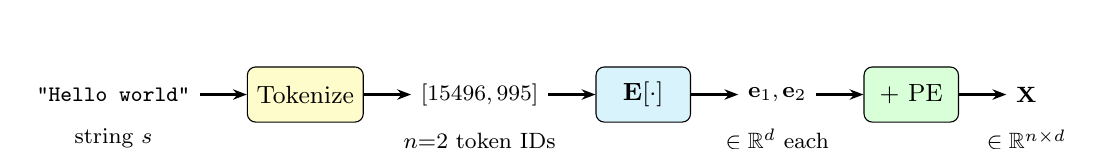
\begin{tikzpicture}[
    node distance=0.8cm,
    box/.style={draw, rounded corners=3pt, minimum height=0.7cm, minimum width=1.2cm, font=\small},
    arrow/.style={-{Stealth[length=5pt]}, thick},
    label/.style={font=\footnotesize, text=black}
  ]
  % Nodes
  \node[label] (str) {$\texttt{"Hello world"}$};
  \node[label, below=0.1cm of str] (strlbl) {\footnotesize string $s$};

  \node[box, fill=yellow!20, right=0.6cm of str] (tok) {Tokenize};
  \node[label, right=0.6cm of tok] (ids) {$[15496, 995]$};
  \node[label, below=0.1cm of ids] (idslbl) {\footnotesize $n{=}2$ token IDs};

  \node[box, fill=cyan!15, right=0.6cm of ids] (emb) {$\mathbf{E}[\cdot]$};
  \node[label, right=0.6cm of emb] (vecs) {$\mathbf{e}_1, \mathbf{e}_2$};
  \node[label, below=0.1cm of vecs] (vecslbl) {\footnotesize $\in \mathbb{R}^d$ each};

  \node[box, fill=green!15, right=0.6cm of vecs] (pe) {$+$ PE};
  \node[label, right=0.6cm of pe] (X) {$\mathbf{X}$};
  \node[label, below=0.1cm of X] (Xlbl) {\footnotesize $\in \mathbb{R}^{n \times d}$};

  % Arrows
  \draw[arrow] (str) -- (tok);
  \draw[arrow] (tok) -- (ids);
  \draw[arrow] (ids) -- (emb);
  \draw[arrow] (emb) -- (vecs);
  \draw[arrow] (vecs) -- (pe);
  \draw[arrow] (pe) -- (X);
\end{tikzpicture}
\caption{The input pipeline for a concrete example. The string is tokenized into integer IDs, each ID is looked up in the embedding table to produce a $d$-dimensional vector, and positional encodings are added element-wise. The result is the matrix $\mathbf{X}$ that enters the first transformer block.}
\label{fig:input-pipeline}
\end{figure}


\section{The Attention Mechanism}
\label{sec:attention-mechanism}

The input matrix $\mathbf{X}$ tells us what each token \emph{is} and where it appears, but it says nothing about how tokens relate to each other. In the sentence ``The cat sat on the mat because \emph{it} was tired,'' the word ``it'' refers to ``cat''---but a bag of independent embedding vectors has no way to express that. The \emph{attention mechanism} is how the transformer lets every token look at every other token and decide which ones are relevant.


\subsection{The Library Analogy}

Before we introduce any math, consider a library. You walk in with a \emph{question} in mind (``I need information about quantum physics''). Every book on every shelf has an \emph{index card} describing its contents (``Introduction to Quantum Mechanics,'' ``A History of France,'' ``Cooking Italian''). And each book has its actual \emph{content}---the pages inside.

To find what you need, you compare your question against every index card. Some cards match well (the quantum mechanics book), some match partially (a general physics overview), and most do not match at all (the cookbook). You then read from the matching books, weighting your reading time in proportion to how well each card matched your question. The result is an answer assembled from the most relevant sources.

Attention works exactly this way:
\begin{itemize}
  \item $\mathbf{Q}$ \textbf{(Query)} = the question you are asking. Each token generates a query vector that represents ``what am I looking for?''
  \item $\mathbf{K}$ \textbf{(Key)} = the index card on each book. Each token generates a key vector that represents ``what do I contain?''
  \item $\mathbf{V}$ \textbf{(Value)} = the book's content. Each token generates a value vector that represents ``here is my information.''
\end{itemize}
Comparing a query against all keys tells us \emph{where to look}. Reading from the corresponding values tells us \emph{what to gather}. The output for each token is a weighted combination of all the value vectors, where the weights come from query-key comparisons.


\subsection{From Analogy to Math}

Each token's embedding vector $\mathbf{x}_i \in \mathbb{R}^d$ is projected through three learned weight matrices to produce the query, key, and value vectors:\footnote{We follow the convention of Vaswani et al.\ and write $\mathbf{x}_i\mathbf{W}$ (row vector $\times$ matrix) rather than the $\mathbf{W}\mathbf{x}_i$ (matrix $\times$ column vector) more common in linear algebra textbooks. The row-vector convention extends naturally to batches: stacking $n$ tokens into $\mathbf{X} \in \mathbb{R}^{n \times d}$ gives $\mathbf{Q} = \mathbf{X}\mathbf{W}^Q \in \mathbb{R}^{n \times d_k}$ directly, with no transposes needed.}
\begin{align}
\mathbf{q}_i &= \mathbf{x}_i \mathbf{W}^Q, & \mathbf{W}^Q &\in \mathbb{R}^{d \times d_k} \\
\mathbf{k}_i &= \mathbf{x}_i \mathbf{W}^K, & \mathbf{W}^K &\in \mathbb{R}^{d \times d_k} \\
\mathbf{v}_i &= \mathbf{x}_i \mathbf{W}^V, & \mathbf{W}^V &\in \mathbb{R}^{d \times d_v}
\end{align}
where $\mathbf{W}^Q$, $\mathbf{W}^K$, and $\mathbf{W}^V$ are the learned projection matrices, $d_k$ is the dimension of keys and queries, and $d_v$ is the dimension of values (in the original transformer, $d_k = d_v = 64$).

Why must queries and keys share the dimension $d_k$, while values are free to use a different $d_v$? Because attention computes the dot product $\mathbf{q}_i \cdot \mathbf{k}_j$ to measure relevance---and a dot product requires both vectors to have the same number of elements. In matrix form, $\mathbf{Q}\mathbf{K}^\top$ multiplies an $n \times d_k$ matrix by a $d_k \times n$ matrix; if their inner dimensions disagreed, the multiplication would be undefined. Values, by contrast, are never compared to queries or keys---they are simply weighted and summed---so $d_v$ is an independent design choice.

\textbf{Stacking into matrices.}\hspace{1em} Each token $i$ produces its own row vectors $\mathbf{q}_i$, $\mathbf{k}_i$, $\mathbf{v}_i$. For $n$ tokens we stack these rows to form the full matrices:
\begin{equation}
\mathbf{Q} = \mathbf{X}\mathbf{W}^Q \in \mathbb{R}^{n \times d_k}, \qquad
\mathbf{K} = \mathbf{X}\mathbf{W}^K \in \mathbb{R}^{n \times d_k}, \qquad
\mathbf{V} = \mathbf{X}\mathbf{W}^V \in \mathbb{R}^{n \times d_v}
\end{equation}

This is the same per-token projection from Equation~2.7, written as a single matrix multiplication. Because $\mathbf{X} \in \mathbb{R}^{n \times d}$ has one row per token, multiplying by $\mathbf{W}^Q \in \mathbb{R}^{d \times d_k}$ applies the projection to every token simultaneously---row $i$ of the result is exactly $\mathbf{q}_i = \mathbf{x}_i\mathbf{W}^Q$. With these three matrices in hand, we can compute attention for all tokens at once:
\begin{equation}
\label{eq:attention}
\text{Attention}(\mathbf{Q}, \mathbf{K}, \mathbf{V}) = \text{softmax}\!\left(\frac{\mathbf{Q}\mathbf{K}^\top}{\sqrt{d_k}}\right)\mathbf{V}
\end{equation}

This is the \emph{scaled dot-product attention} formula from Vaswani et al.\ (2017).\footnote{Ashish Vaswani, Noam Shazeer, Niki Parmar, Jakob Uszkoreit, Llion Jones, Aidan N.\ Gomez, {\L}ukasz Kaiser, and Illia Polosukhin, ``Attention Is All You Need,'' \emph{NeurIPS}, 2017.} Let us break it apart step by step.

\textbf{Step 1: Dot products.}\hspace{1em} The matrix product $\mathbf{Q}\mathbf{K}^\top$ produces an $n \times n$ matrix of \emph{attention scores}. Entry $(i, j)$ is the dot product $\mathbf{q}_i \cdot \mathbf{k}_j$---a scalar measuring how well token $i$'s query matches token $j$'s key. A large positive score means token $j$ is highly relevant to token $i$; a score near zero means it is irrelevant.

\marginnote{\emph{Scaling:} dividing by $\sqrt{d_k}$ prevents dot products from growing too large as the dimension increases.}%
\textbf{Step 2: Scaling by $\sqrt{d_k}$.}\hspace{1em} The dot products are divided by $\sqrt{d_k}$. Without this scaling, dot-product magnitudes grow with the dimension $d_k$, pushing softmax into a saturated regime where it places nearly all weight on a single token and gradients vanish. Dividing by $\sqrt{d_k}$ normalizes the variance of the dot products back to 1, keeping softmax well-behaved regardless of the model's choice of $d_k$.

\begin{notebox}
\textbf{Why $\sqrt{d_k}$: the variance argument.} The entries of $\mathbf{q}_i$ and $\mathbf{k}_j$ are deterministic outputs of learned projections, not truly random. But treating individual entries as draws from some distribution is the standard device for understanding how magnitudes scale with dimensionality.

We use three indices throughout this derivation:
\begin{itemize}
  \item $i$ --- the \textbf{query position}: which token is asking ``what should I attend to?''
  \item $j$ --- the \textbf{key position}: which token is being considered as an attention target
  \item $m$ --- the \textbf{dimension index} within the $d_k$-dimensional query/key vectors ($m = 1, \ldots, d_k$)
\end{itemize}
So $q_{i,m}$ is the $m$-th component of the query vector at position $i$, and $k_{j,m}$ is the $m$-th component of the key vector at position $j$.

\emph{The key result:} without scaling, the variance of the dot product grows proportionally to $d_k$, causing softmax to saturate to a near-one-hot distribution. We now derive this step by step.

Suppose each entry $q_{i,m}$ is an independent random variable with $\mathbb{E}[q_{i,m}] = \mu_q$, $\text{Var}(q_{i,m}) = \sigma^2$, and likewise $\mathbb{E}[k_{j,m}] = \mu_k$, $\text{Var}(k_{j,m}) = \sigma^2$. The dot product is:
\[
\mathbf{q}_i \cdot \mathbf{k}_j = \sum_{m=1}^{d_k} q_{i,m}\, k_{j,m}
\]

Each term $q_{i,m}\, k_{j,m}$ is the product of two independent random variables. Its mean is:
\[
\mathbb{E}[q_{i,m}\, k_{j,m}] = \mathbb{E}[q_{i,m}]\,\mathbb{E}[k_{j,m}] = \mu_q \mu_k
\]

For the variance, we use $\text{Var}(q_{i,m}\, k_{j,m}) = \mathbb{E}[(q_{i,m}\, k_{j,m})^2] - (\mathbb{E}[q_{i,m}\, k_{j,m}])^2$. By independence:
\[
\mathbb{E}[(q_{i,m}\, k_{j,m})^2] = \mathbb{E}[q_{i,m}^2]\,\mathbb{E}[k_{j,m}^2] = (\sigma^2 + \mu_q^2)(\sigma^2 + \mu_k^2)
\]
where we used $\mathbb{E}[q_{i,m}^2] = \text{Var}(q_{i,m}) + (\mathbb{E}[q_{i,m}])^2 = \sigma^2 + \mu_q^2$. Subtracting:
\[
\text{Var}(q_{i,m}\, k_{j,m}) = (\sigma^2 + \mu_q^2)(\sigma^2 + \mu_k^2) - \mu_q^2 \mu_k^2 = \sigma^4 + \sigma^2(\mu_q^2 + \mu_k^2)
\]

Since the $d_k$ terms are independent:
\begin{align}
\mathbb{E}[\mathbf{q}_i \cdot \mathbf{k}_j] &= d_k\, \mu_q \mu_k \\
\text{Var}(\mathbf{q}_i \cdot \mathbf{k}_j) &= d_k[\sigma^4 + \sigma^2(\mu_q^2 + \mu_k^2)]
\end{align}

Both the mean and the variance grow linearly with $d_k$. The standard deviation grows as $\sqrt{d_k}$---regardless of $\mu_q$, $\mu_k$, or $\sigma$, this is the dimension-dependent factor. In the original transformer, $d_k = 64$ contributes $\sqrt{64} = 8$; modern models with $d_k = 128$ contribute $\approx 11.3$.

\emph{Why this causes softmax saturation.} Softmax is sensitive to input magnitude. When values are moderate (range $[-3, 3]$), it produces a ``soft'' distribution that spreads weight across tokens. But when one value dominates (say, $z_j = 20$ while others are near 0), the exponential $e^{20} \approx 5 \times 10^8$ overwhelms all other terms, producing an effectively one-hot output. In this saturated regime, gradients $\partial\text{softmax}/\partial z_j$ become extremely small, stalling learning.

\emph{The fix.} Dividing by $\sqrt{d_k}$ removes the dimension-dependent factor. For any constant $c$, $\text{Var}(X/c) = \text{Var}(X)/c^2$ and $\mathbb{E}[X/c] = \mathbb{E}[X]/c$. Applying this with $c = \sqrt{d_k}$:
\begin{align}
\text{Var}\!\left(\frac{\mathbf{q}_i \cdot \mathbf{k}_j}{\sqrt{d_k}}\right) &= \frac{d_k[\sigma^4 + \sigma^2(\mu_q^2 + \mu_k^2)]}{d_k} = \sigma^4 + \sigma^2(\mu_q^2 + \mu_k^2) \\
\mathbb{E}\!\left[\frac{\mathbf{q}_i \cdot \mathbf{k}_j}{\sqrt{d_k}}\right] &= \frac{d_k\, \mu_q \mu_k}{\sqrt{d_k}} = \sqrt{d_k}\, \mu_q \mu_k
\end{align}

The variance no longer grows with $d_k$. The mean does still grow---but this is harmless. To see why, fix a query position $i$ and ask how the score $z_{ij}$ varies across different key positions $j$. Decompose each component as its mean plus a deviation:
\[
q_{i,m} = \mu_q + \delta^q_{i,m}, \qquad k_{j,m} = \mu_k + \delta^k_{j,m}
\]
where $\sum_m \delta^q_{i,m} = 0$ and $\sum_m \delta^k_{j,m} = 0$ by definition of the mean. Now expand a single term of the dot product:
\[
q_{i,m}\, k_{j,m} = (\mu_q + \delta^q_{i,m})(\mu_k + \delta^k_{j,m}) = \mu_q \mu_k + \mu_q\, \delta^k_{j,m} + \mu_k\, \delta^q_{i,m} + \delta^q_{i,m}\, \delta^k_{j,m}
\]

Summing over all $d_k$ dimensions and dividing by $\sqrt{d_k}$:
\begin{equation}
z_{ij} = \frac{\mathbf{q}_i \cdot \mathbf{k}_j}{\sqrt{d_k}} = \frac{1}{\sqrt{d_k}}\left[\underbrace{d_k\, \mu_q \mu_k}_{\text{mean--mean}} + \mu_q \underbrace{\sum_m \delta^k_{j,m}}_{= 0} + \mu_k \underbrace{\sum_m \delta^q_{i,m}}_{= 0} + \sum_m \delta^q_{i,m}\, \delta^k_{j,m}\right]
\end{equation}
\[
= \underbrace{\sqrt{d_k}\; \mu_q \mu_k}_{\text{depends on component means}} + \underbrace{\frac{1}{\sqrt{d_k}} \sum_{m=1}^{d_k} \delta^q_{i,m}\, \delta^k_{j,m}}_{\text{depends on per-component structure}}
\]

The two cross terms vanish because the deviations sum to zero by construction. This is a purely deterministic decomposition---it holds for any specific vectors $\mathbf{q}_i$ and $\mathbf{k}_j$, not just in expectation.

The first term, $\sqrt{d_k}\, \mu_q \mu_k$, depends only on the component means of $\mathbf{q}_i$ and $\mathbf{k}_j$. Note that $\mu_k$ is the mean of $\mathbf{k}_j$'s components and does vary with $j$---but in Pre-LN transformers (as discussed below), layer normalization drives both $\mu_q \approx 0$ and $\mu_k \approx 0$, making this term negligible for all $j$. When this holds, attention weights are determined entirely by the second term. More generally, softmax is shift-invariant: for any constant $c$,
\[
\text{softmax}(z_{ij} + c) = \frac{e^{z_{ij}+c}}{\sum_\ell e^{z_{i\ell}+c}} = \frac{e^c\, e^{z_{ij}}}{e^c \sum_\ell e^{z_{i\ell}}} = \frac{e^{z_{ij}}}{\sum_\ell e^{z_{i\ell}}} = \text{softmax}(z_{ij})
\]
so any term that is the same for all $j$ has no effect on the attention weights. When $\mu_q \approx 0$ (the Pre-LN regime), the first term dominates. The variance of $z_{ij}$---driven by this second term---is exactly what we computed in Equation~2.14: $\sigma^4 + \sigma^2(\mu_q^2 + \mu_k^2)$, with no dependence on $d_k$.

\emph{What are $\mu$ and $\sigma^2$ in practice?} In Pre-LN transformers, layer normalization\footnote{Layer normalization explicitly centers each token's vector to zero mean and scales it to unit variance (before the learned affine parameters $\boldsymbol{\gamma}$ and $\boldsymbol{\beta}$). Since this is applied \emph{before} the $\mathbf{W}^Q$ and $\mathbf{W}^K$ projections, the inputs to those projections have $\mu \approx 0$. This makes the $\mu$-dependent terms in Equations~2.12--2.13 negligible in practice.} is applied before the Q/K/V projections, centering the input to approximately zero mean. Xavier/Glorot initialization (2010) then sets each weight entry in $\mathbf{W}^Q$ to have variance $1/d$. Since $q_{i,m} = \sum_{r=1}^{d} x_{i,r}\, W^Q_{r,m}$ and the layer-normalized input has approximately zero mean and unit variance, we get $\mu_q \approx 0$ and $\text{Var}(q_{i,m}) \approx d \cdot (1 \cdot 1/d) = 1$. So at the start of training, $\mu \approx 0$ and $\sigma^2 \approx 1$, giving $\text{Var}(\mathbf{q} \cdot \mathbf{k}) \approx d_k$---and dividing by $\sqrt{d_k}$ restores unit variance. After training, layer normalization continues to keep the projection inputs well-scaled.
\end{notebox}

\marginnote{\emph{Softmax:} converts a vector of arbitrary real numbers into a probability distribution (all positive, summing to 1).}%
\textbf{Step 3: Softmax.}\hspace{1em} The softmax function converts each row of the scaled score matrix into a probability distribution---a vector of non-negative weights that sum to 1:
\begin{equation}
\text{softmax}(z_j) = \frac{e^{z_j}}{\sum_{i=1}^{n} e^{z_\ell}}
\end{equation}
where $e^{z_j}$ is the exponential of the $j$-th element, and the denominator sums the exponentials of all elements. After softmax, each row of the score matrix is a \emph{probability distribution} over all tokens. Token $i$'s row tells us how much ``attention'' token $i$ should pay to each token in the sequence. If token $i$'s query matches token $j$'s key far better than any other key, the softmax weight for position $j$ will be close to 1 and all others close to 0. If several keys match equally well, the weights will be spread more evenly.

\begin{notebox}
\textbf{Why softmax?} After scaling, each row of the score matrix contains $n$ real numbers that can be positive, negative, or zero. But we need \emph{weights} for a weighted average: coefficients that are (1) non-negative (a negative weight would mean ``pay anti-attention,'' which has no clear interpretation), and (2) sum to 1 (so the output is a proper average). Raw dot-product scores satisfy neither requirement.

We could normalize the scores by dividing each by their sum, but this fails when scores are negative---and dot products are frequently negative. We need a function that maps arbitrary real numbers to positive values while preserving relative ordering.

The exponential function $e^z$ does exactly this: it maps any real number to a strictly positive value ($e^z > 0$ for all $z$), is monotonically increasing (larger inputs give larger outputs), and amplifies differences (the gap between $e^3$ and $e^1$ is much larger than $3 - 1$). Normalizing the exponentiated values by their sum gives softmax.

The name comes from the fact that softmax is a ``soft'' version of $\arg\max$. Whereas $\arg\max$ puts all weight on the single largest element (a hard, all-or-nothing choice), softmax puts \emph{most} weight on the largest but distributes some to others in proportion to their scores. This smoothness is essential: softmax is differentiable everywhere, which the model needs for learning through gradient descent.
\end{notebox}

\textbf{Step 4: Weighted sum.}\hspace{1em} Multiplying the softmax output by $\mathbf{V}$ computes a weighted average of the value vectors for each token. Writing $\alpha_{ij}$ for the softmax weight that token $i$ places on token $j$ (i.e., entry $(i, j)$ of the softmax matrix), the output for token $i$ is:
\begin{equation}
\underbrace{\mathbf{o}_i}_{1 \times d_v} = \sum_{j=1}^{n} \underbrace{\alpha_{ij}}_{\text{scalar}} \;\underbrace{\mathbf{v}_j}_{1 \times d_v}
\end{equation}

Each $\alpha_{ij}$ is a scalar weight; each $\mathbf{v}_j$ is a $d_v$-dimensional row vector; the output $\mathbf{o}_i$ is their weighted sum, also $d_v$-dimensional. Stacking all $n$ rows into a single matrix multiplication gives the vector form:
\begin{equation}
\underbrace{\mathbf{O}}_{n \times d_v} = \underbrace{\boldsymbol{\alpha}}_{n \times n}\; \underbrace{\mathbf{V}}_{n \times d_v}
\end{equation}
where $\boldsymbol{\alpha} = \text{softmax}\!\left(\mathbf{Q}\mathbf{K}^\top / \sqrt{d_k}\right)$. Row $i$ of $\boldsymbol{\alpha}$ is the probability distribution over key positions for query $i$; multiplying by $\mathbf{V}$ takes the weighted average of value vectors according to that distribution, producing row $i$ of $\mathbf{O}$.

If token $i$ attends mostly to token $j$ (i.e., $\alpha_{ij}$ is large), then the output $\mathbf{o}_i$ will be close to $\mathbf{v}_j$. In practice, the output is a blend of many value vectors, weighted by relevance.

\begin{figure}[h]
\centering
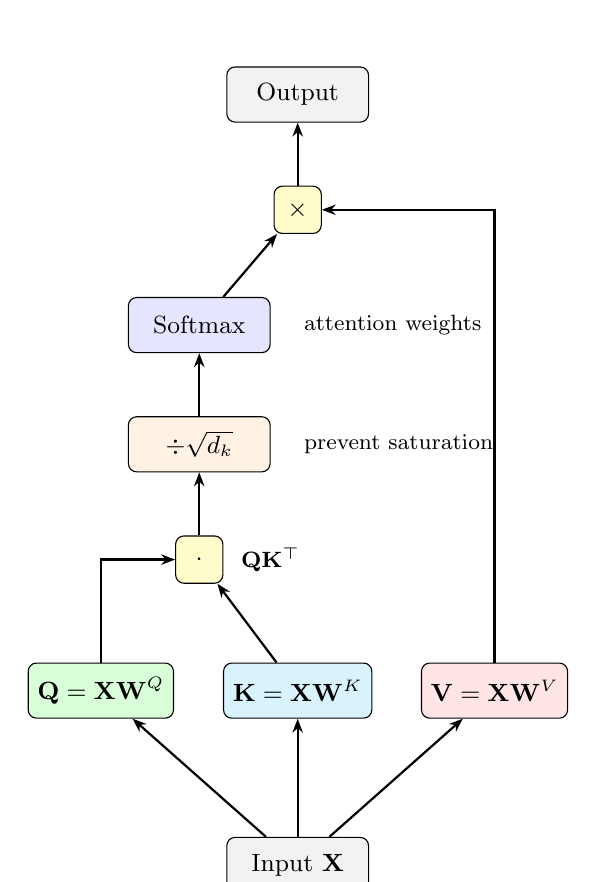
\begin{tikzpicture}[
    node distance=1cm,
    box/.style={draw, rounded corners=3pt, minimum height=0.7cm, minimum width=1.8cm, font=\small},
    smallbox/.style={draw, rounded corners=3pt, minimum height=0.6cm, minimum width=0.6cm, font=\small},
    arrow/.style={-{Stealth[length=5pt]}, thick},
    label/.style={font=\footnotesize}
  ]
  % Input
  \node[box, fill=gray!10] (input) {Input $\mathbf{X}$};

  % Q, K, V
  \node[box, fill=green!15, above=1.5cm of input, xshift=-2.5cm] (Q) {$\mathbf{Q} = \mathbf{X}\mathbf{W}^Q$};
  \node[box, fill=cyan!15, above=1.5cm of input] (K) {$\mathbf{K} = \mathbf{X}\mathbf{W}^K$};
  \node[box, fill=red!10, above=1.5cm of input, xshift=2.5cm] (V) {$\mathbf{V} = \mathbf{X}\mathbf{W}^V$};

  % Dot product
  \node[smallbox, fill=yellow!20, above=1cm of K, xshift=-1.25cm] (dot) {$\cdot$};
  \node[label, right=0.1cm of dot] {$\mathbf{Q}\mathbf{K}^\top$};

  % Scale
  \node[box, fill=orange!10, above=0.8cm of dot] (scale) {$\div \sqrt{d_k}$};
  \node[label, right=0.3cm of scale] {\footnotesize prevent saturation};

  % Softmax
  \node[box, fill=blue!10, above=0.8cm of scale] (softmax) {Softmax};
  \node[label, right=0.3cm of softmax] {\footnotesize attention weights};

  % Multiply
  \node[smallbox, fill=yellow!20, above=0.8cm of softmax, xshift=1.25cm] (mult) {$\times$};

  % Output
  \node[box, fill=gray!10, above=0.8cm of mult] (output) {Output};

  % Arrows
  \draw[arrow] (input) -- (Q);
  \draw[arrow] (input) -- (K);
  \draw[arrow] (input) -- (V);
  \draw[arrow] (Q) |- (dot);
  \draw[arrow] (K) -- (dot);
  \draw[arrow] (dot) -- (scale);
  \draw[arrow] (scale) -- (softmax);
  \draw[arrow] (softmax) -- (mult);
  \draw[arrow] (V) |- (mult);
  \draw[arrow] (mult) -- (output);
\end{tikzpicture}
\caption{Scaled dot-product attention for a single head. The input $\mathbf{X}$ is projected into queries, keys, and values. Queries and keys are compared via dot product, scaled, and passed through softmax to produce attention weights. These weights select a mixture of value vectors to form the output.}
\label{fig:attention}
\end{figure}

\textbf{Why $n \times n$ matters.}\hspace{1em} The attention score matrix has $n^2$ entries, where $n$ is the sequence length. This means the computational cost of attention grows \emph{quadratically} with sequence length: a sequence of 4,096 tokens produces a $4096 \times 4096$ score matrix with roughly 16.8 million entries. At 8,192 tokens, that number quadruples to 67 million. This quadratic scaling is the fundamental reason why long-context inference is expensive, and it motivates many of the optimizations we will see in later chapters.

\begin{notebox}
\textbf{Causal masking.} In language models used for generation, token $i$ should only attend to tokens at positions $\leq i$---it must not ``see the future.'' This is enforced by adding a \emph{causal mask}: the upper-triangular entries of the score matrix (where $j > i$) are set to $-\infty$ before softmax, causing them to become zero after exponentiation. The mask does not change the formula; it just ensures that information flows only from earlier tokens to later ones.
\end{notebox}

\begin{notebox}
\textbf{If attention requires an $n \times n$ matrix, how do models handle 128K-token contexts?}

The $n^2$ scaling described above is real, but a critical implementation insight makes it far less painful than it sounds. Standard attention computes the full $n \times n$ score matrix in HBM, applies softmax, then multiplies by $\mathbf{V}$---requiring $O(n^2)$ memory and $\Theta(n^2 d + n^2)$ HBM accesses. \textbf{FlashAttention}\footnote{Tri Dao, Daniel Y.\ Fu, Stefano Ermon, Atri Rudra, and Christopher R\'{e}, ``FlashAttention: Fast and Memory-Efficient Exact Attention with IO-Awareness,'' \emph{NeurIPS}, 2022.} eliminates the need to ever materialize this matrix. The key insight: attention can be computed \emph{block by block}, accumulating the result incrementally, without changing the mathematical output.

\emph{The memory hierarchy problem.} A GPU has two levels of memory that matter: \textbf{HBM} (high-bandwidth memory, e.g., 80\,GB on an A100, $\sim$2\,TB/s) and \textbf{SRAM} (on-chip shared memory, e.g., 20\,MB total across all streaming multiprocessors, $\sim$19\,TB/s). SRAM is roughly 10$\times$ faster but 4,000$\times$ smaller. Standard attention writes the entire $n \times n$ score matrix to HBM (because it doesn't fit in SRAM), reads it back for softmax, writes the softmax output, and reads it again for the matrix multiply with $\mathbf{V}$. Each of these round-trips to HBM is expensive.

\emph{Tiling.} FlashAttention partitions $\mathbf{Q}$, $\mathbf{K}$, and $\mathbf{V}$ into blocks that fit in SRAM. For each block of queries $\mathbf{Q}_i$ and each block of keys/values $(\mathbf{K}_j, \mathbf{V}_j)$, it computes the local score block $\mathbf{Q}_i \mathbf{K}_j^\top$, applies scaling and masking, and accumulates the partial attention output---all within SRAM, with no writes to HBM until the final result is ready.

\emph{The online softmax trick.} The challenge is that softmax is a \emph{global} operation: $\alpha_{ij} = e^{z_{ij}} / \sum_\ell e^{z_{i\ell}}$ requires knowing all scores $z_{i\ell}$ before normalizing any of them. FlashAttention solves this by maintaining two running statistics per query row: the running maximum $m$ (for numerical stability) and the running sum of exponentials $\ell$. As each new key block is processed, these statistics are updated and the partial output is \emph{rescaled} to account for the new normalization. After all key blocks have been processed, the accumulated output is exactly the same as standard attention---no approximation.

Concretely, after processing key blocks $1, \ldots, j{-}1$, the algorithm holds:
\begin{align*}
m^{(j-1)} &= \max_{k \leq j-1} \max_c\; z_{ic}, \\
\ell^{(j-1)} &= \sum_{k \leq j-1} \sum_c e^{z_{ic} - m^{(j-1)}}, \\
\mathbf{o}^{(j-1)} &= \frac{1}{\ell^{(j-1)}} \sum_{k \leq j-1} \sum_c e^{z_{ic} - m^{(j-1)}} \mathbf{v}_c
\end{align*}

When key block $j$ arrives with new scores, the maximum may increase ($m^{(j)} \geq m^{(j-1)}$), so the running sum and output must be rescaled by $e^{m^{(j-1)} - m^{(j)}}$ before incorporating the new block's contribution. This rescaling is the core of the online softmax algorithm.

\emph{IO complexity.} Standard attention performs $\Theta(n\,d_k + n^2)$ HBM accesses (reading/writing $\mathbf{Q}$, $\mathbf{K}$, $\mathbf{V}$ and the $n \times n$ score matrices). FlashAttention reduces this to $\Theta(n^2 d_k^2/M)$ where $M$ is SRAM size. For typical values ($d_k = 128$, $M \approx 100$\,KB), this is a substantial reduction---up to 7.6$\times$ faster than standard PyTorch attention on GPT-2 scale models.

\emph{What FlashAttention does \textbf{not} change.} The output is \emph{bit-for-bit identical} to standard attention. FlashAttention is not an approximation---it computes the exact same $\text{softmax}(\mathbf{Q}\mathbf{K}^\top / \sqrt{d_k})\,\mathbf{V}$. It is purely an optimization of the \emph{execution order}: instead of materializing intermediate matrices in slow HBM, it keeps everything in fast SRAM and accumulates the result incrementally.

\textbf{FlashAttention-2}\footnote{Tri Dao, ``FlashAttention-2: Faster Attention with Better Parallelism and Work Partitioning,'' \emph{ICLR}, 2024.} improved upon the original with two key changes: (1) \emph{reduced non-matmul FLOPs} by restructuring the online softmax to minimize rescaling operations, and (2) \emph{better warp partitioning}---in FlashAttention-1, the $\mathbf{K}$ and $\mathbf{V}$ blocks were split across GPU warps (requiring synchronization to combine results), while FlashAttention-2 splits $\mathbf{Q}$ across warps instead, so each warp independently computes its slice of the output with no inter-warp communication. This yielded $\sim$2$\times$ speedup, reaching 50--73\% of theoretical peak FLOPS on A100.

\textbf{FlashAttention-3}\footnote{Jay Shah, Ganesh Bikshandi, Ying Zhang, Vijay Thakkar, Pradeep Ramani, and Tri Dao, ``FlashAttention-3: Fast and Accurate Attention with Asynchrony and Low-precision,'' \emph{NeurIPS}, 2024.} targets NVIDIA's Hopper architecture (H100) and exploits three hardware features: (1) \emph{warp specialization}---dedicating some warps to data movement (via the Tensor Memory Accelerator) and others to computation (via WGMMA instructions), overlapping the two; (2) \emph{interleaved block-wise computation}---pipelining the softmax of one block with the matrix multiply of the next; and (3) \emph{FP8 low-precision} with \emph{incoherent processing}---multiplying by a random orthogonal matrix to spread quantization error across dimensions, reducing error by 2.6$\times$ compared to na\"ive FP8. The result: up to 740\,TFLOPS in FP16 (75\% of H100 peak, up from 35\% with FlashAttention-2) and 1.2\,PFLOPS in FP8.

\emph{Context window implications.} FlashAttention's $O(n)$ memory (instead of $O(n^2)$) is what makes 100K+ context windows feasible on current hardware. Without it, a 128K-token sequence would require a $128\text{K} \times 128\text{K}$ score matrix---roughly 32\,GB in FP16 \emph{per attention head, per layer}. With FlashAttention, the memory cost is linear in $n$ (only the output and the running statistics are stored), and the remaining quadratic cost is purely in \emph{compute}, which modern GPUs handle well for moderate $n$.

That said, models are trained with a fixed maximum context length (e.g., 8K for the original LLaMA, 128K for newer models). Beyond this length, attention patterns degrade because the positional encodings were never seen at those distances during training. Techniques like RoPE scaling partially address this by interpolating or extrapolating the learned frequencies, but some quality loss at extreme lengths remains an active research problem.
\end{notebox}


\subsection{Why Three Separate Projections?}

In Section~2.2.2, we introduced $\mathbf{W}^Q$, $\mathbf{W}^K$, and $\mathbf{W}^V$ as projection matrices that produce queries, keys, and values. But why project at all? Why not compare the raw embeddings $\mathbf{x}_i$ directly---compute $\mathbf{x}_i \cdot \mathbf{x}_j$ as the attention score, and use $\mathbf{x}_j$ itself as the value? Three independent reasons make this insufficient.

\begin{notebox}
\textbf{Skip on first reading.} This section is a deep dive into why the Q/K/V projection structure exists. If you are reading this chapter for the first time, you may wish to skip ahead to Section~\ref{sec:multihead} (Multi-Head Attention) and return here later. The rest of the guide does not depend on this material.
\end{notebox}

\textbf{Projections separate identity from intent.}\hspace{1em} The embedding $\mathbf{x}_i$ encodes what token $i$ \emph{is}---its lexical identity, syntactic category, and semantic associations. But attention needs to answer a different question: what is token $i$ \emph{looking for}? These are not the same thing. The embedding of ``sat'' encodes \emph{I am a past-tense verb meaning to be seated}. But what ``sat'' needs from the sequence is a subject noun phrase---something categorically different from itself. Without $\mathbf{W}^Q$, every token's query would just be its own embedding, and attention would reduce to ``find tokens similar to me.'' A verb would attend most strongly to other verbs (since their embeddings cluster together), not to its syntactic arguments.

$\mathbf{W}^Q$ transforms identity into a search criterion: ``I am a verb'' $\to$ ``I need a noun phrase subject.'' $\mathbf{W}^K$ transforms identity into an advertisement: ``I am a noun'' $\to$ ``I am available as a subject or object.'' The dot product $\mathbf{q}_i \cdot \mathbf{k}_j$ then measures how well $j$'s advertisement matches $i$'s search---not how similar $i$ and $j$ are as tokens.

\textbf{Value projections decouple matching from extraction.}\hspace{1em} Even after we decide that token $i$ should attend heavily to token $j$, a separate question remains: what information should $j$ actually send to $i$? Without $\mathbf{W}^V$, the weighted sum would use $\alpha_{ij} \cdot \mathbf{x}_j$---the same representation that determined relevance would also carry the information payload. This forces a single vector to serve two masters: the features that make ``bank'' \emph{relevant} to ``steep'' (terrain/geography associations, for disambiguation) may differ from the features ``steep'' needs to \emph{extract} from ``bank'' (syntactic role, semantic sense, positional information for downstream layers). Optimizing one objective degrades the other.

$\mathbf{W}^V$ creates a third, independent view of each token. The attention weights $\alpha_{ij} = \text{softmax}\!\left(\mathbf{Q}\mathbf{K}^\top / \sqrt{d_k}\right)_{ij}$ (the $(i,j)$ entry of the softmax output in Eq.~2.11) determine \emph{who} to attend to. The values $\mathbf{v}_j = \mathbf{x}_j \mathbf{W}^V$ determine \emph{what information flows}. These are optimized independently---no interference between objectives.

\textbf{Projections define a learned, low-rank similarity function.}\hspace{1em} Raw dot products compute one fixed geometric relationship: how aligned two vectors are. But ``relevant'' means different things in different contexts---syntactic dependency, coreference, topical similarity, positional proximity. Projections make similarity \emph{learnable}. Expanding the attention score:
\begin{equation}
\mathbf{q}_i \cdot \mathbf{k}_j \;=\; (\mathbf{x}_i \mathbf{W}^Q)(\mathbf{x}_j \mathbf{W}^K)^\top \;=\; \mathbf{x}_i \underbrace{\mathbf{W}^Q {\mathbf{W}^K}^\top}_{\mathbf{M}} \mathbf{x}_j^\top
\end{equation}

\marginnote{\emph{Bilinear form:} a function of two vectors that is linear in each argument separately, producing a scalar. Here: $\mathbf{x}_i \mathbf{M} \mathbf{x}_j^\top$.}%
the product $\mathbf{M} = \mathbf{W}^Q {\mathbf{W}^K}^\top \in \mathbb{R}^{d \times d}$ is a learned matrix that defines the model's task-specific notion of ``relevant.'' This is a \emph{bilinear form}: a function that takes two vectors and produces a scalar, parameterized by $\mathbf{M}$. The model learns which dimensions of the embedding space matter for determining relevance.

Crucially, $\mathbf{M}$ has rank at most $d_k$. It is the product of a $d \times d_k$ matrix ($\mathbf{W}^Q$) and a $d_k \times d$ matrix (${\mathbf{W}^K}^\top$), so its rank cannot exceed $\min(d, d_k) = d_k$. With $d = 4096$ and $d_k = 128$, this means attention computes similarity in a 128-dimensional \emph{subspace} of the full 4096-dimensional embedding space. The model is forced to identify the 128 most informative directions for relevance and discard the rest---a form of structural regularization built directly into the architecture.

\begin{notebox}
\textbf{Nobody programmed these meanings.} A reasonable reaction to the paragraphs above is: ``This sounds like a story imposed after the fact. How do you actually encode into the system that $\mathbf{W}^Q$ should learn `what I'm looking for'?''
You don't. The matrices are initialized randomly and learn whatever minimizes the next-token prediction loss. The labels ``query,'' ``key,'' and ``value'' are human-imposed names borrowed from database terminology---they are not optimization objectives.

But the \emph{roles} are not retroactive interpretation. They are structural facts about the computation graph. $\mathbf{W}^Q$'s output is only ever consumed by a dot product with $\mathbf{W}^K$'s output---it \emph{cannot} carry information to the layer's output. $\mathbf{W}^V$'s output is only ever used in the weighted sum---it \emph{cannot} influence which tokens get attended to. The architecture forces each matrix into exactly one job. What specific patterns each matrix learns within that job (syntactic dependencies, coreference, positional patterns) is discovered by gradient descent and has been empirically verified by researchers who visualized individual attention heads.\footnote{Kevin Clark, Urvashi Khandelwal, Omer Levy, and Christopher D.\ Manning, ``What Does BERT Look At? An Analysis of BERT's Attention,'' \emph{ACL Workshop BlackboxNLP}, 2019.}\textsuperscript{,}\footnote{Elena Voita, David Talbot, Fedor Moiseev, Rico Sennrich, and Ivan Titov, ``Analyzing Multi-Head Self-Attention: Specialized Heads Do the Heavy Lifting, the Rest Can Be Pruned,'' \emph{ACL}, 2019.}

The architecture itself was not a single flash of insight. It evolved over four years of incremental engineering: Bahdanau et al.\ (2014)\footnote{Dzmitry Bahdanau, Kyunghyun Cho, and Yoshua Bengio, ``Neural Machine Translation by Jointly Learning to Align and Translate,'' \emph{ICLR}, 2015 (arXiv 2014).} introduced attention to solve the sequence-to-sequence bottleneck, which already required two separate projections because the decoder and encoder inputs came from different sources. Luong (2015)\footnote{Minh-Thang Luong, Hieu Pham, and Christopher D.\ Manning, ``Effective Approaches to Attention-based Neural Machine Translation,'' \emph{EMNLP}, 2015.} replaced the slow additive scoring with dot products. Several groups applied attention within a single sequence (\emph{self}-attention), which made separate projections necessary rather than optional---without them, $\mathbf{Q} = \mathbf{K} = \mathbf{V} = \mathbf{X}$ and attention reduces to raw similarity. Vaswani et al.\ (2017) removed the recurrent network entirely, showing that attention and feed-forward layers alone suffice. Each step solved a concrete problem; the Q/K/V structure is what you arrive at when the same input must play three structurally distinct roles.
\end{notebox}

\begin{whynotbox}{Why not learn M directly instead of factoring it?}
If the attention score is $\mathbf{x}_i \mathbf{M} \mathbf{x}_j^\top$ and all we need is $\mathbf{M}$, why decompose it into $\mathbf{W}^Q$ and $\mathbf{W}^K$?

\textbf{Parameters.} $\mathbf{M} \in \mathbb{R}^{d \times d}$ has $d^2$ entries. With $d = 4096$: roughly 16.8 million parameters. $\mathbf{W}^Q$ and $\mathbf{W}^K$ together have $2\,d\,d_k$ entries. With $d_k = 128$: roughly 1 million---$16\times$ fewer.

\textbf{Regularization.} $\mathbf{M} = \mathbf{W}^Q {\mathbf{W}^K}^\top$ has rank $\leq d_k$, forcing similarity into a low-dimensional subspace. A full-rank $\mathbf{M}$ could overfit to noise; a rank-128 $\mathbf{M}$ must find structure.

\textbf{Computation.} With separate $\mathbf{Q}$ and $\mathbf{K}$, the intermediates are $n \times d_k$ matrices (compact). With $\mathbf{M}$ directly, the intermediate $\mathbf{X}\mathbf{M}$ is $n \times d$: $32\times$ larger when $d/d_k = 32$, requiring proportionally more memory and arithmetic.

\textbf{Multi-head generalization.} With 32 heads, the factored form needs $32 \times 2 \times d \times d_k \approx 33$M parameters for all heads' query/key projections. Learning 32 separate full $\mathbf{M}$ matrices would require $32 \times d^2 \approx 537$M---over $16\times$ more, with no additional expressiveness.
\end{whynotbox}

\begin{whynotbox}{Why not use an asymmetric operator instead of dot products?}
\textbf{Why asymmetry matters.}\hspace{1em} Attention scores should be directional: ``how much does token $i$ need information from token $j$?'' is a different question from ``how much does token $j$ need information from token $i$?'' Consider the sentence ``\emph{The cat sat on the mat}.'' The pronoun-resolution pattern is a clear example: if ``it'' appeared later, ``it'' would strongly attend to ``cat'' to resolve its referent, but ``cat'' has no comparable need to attend to ``it.'' More generally, a function word like ``the'' contributes little information when attended to, but must itself attend broadly to determine which noun it modifies. A symmetric score function---one where $\text{score}(i,j) = \text{score}(j,i)$ always---cannot capture these directional differences.

The dot product is exactly such a symmetric operator: $\mathbf{x} \cdot \mathbf{y} = \mathbf{y} \cdot \mathbf{x}$, always, in any number of dimensions. This is commutativity of scalar multiplication---a mathematical fact, not a limitation of embedding size. Making embeddings larger cannot fix it.

One could use an inherently asymmetric operator. \emph{Additive attention} (Bahdanau et al., 2014) does exactly this:
\[
\text{score}(i, j) = \mathbf{w}^\top \tanh(\mathbf{W}_1 \mathbf{x}_i + \mathbf{W}_2 \mathbf{x}_j)
\]
where $\mathbf{W}_1$ and $\mathbf{W}_2$ play roles analogous to $\mathbf{W}^Q$ and $\mathbf{W}^K$ (separate learned transformations of the two inputs), $\tanh$ is a nonlinearity, and $\mathbf{w}$ is a learned vector that collapses the result to a scalar. Asymmetry is built in ($\mathbf{W}_1 \neq \mathbf{W}_2$), and this was the standard attention mechanism before the transformer. It works---but it is slow. The difference comes down to what kind of work the GPU is doing:

\marginnote{\emph{Arithmetic intensity} = FLOPs per byte of memory accessed. Higher is better on GPUs.}%
\textbf{Dot-product attention} computes the entire $n \times n$ score matrix as a single matrix multiplication $\mathbf{Q}\mathbf{K}^\top$: an $(n \times d_k) \times (d_k \times n)$ GEMM requiring $2n^2 d_k$ FLOPs. The projections $\mathbf{Q} = \mathbf{X}\mathbf{W}^Q$ and $\mathbf{K} = \mathbf{X}\mathbf{W}^K$ are also GEMMs ($2nd\,d_k$ FLOPs each). The total cost is $4nd\,d_k + 2n^2 d_k$ FLOPs, and every operation is a matrix multiply---the operation that GPU tensor cores are silicon-optimized for. A GEMM of two $m \times m$ matrices performs $O(m^3)$ FLOPs while reading $O(m^2)$ bytes, giving an arithmetic intensity of $O(m)$ FLOPs/byte. For typical sequence lengths this is hundreds of FLOPs per byte---firmly \emph{compute-bound}, which means the GPU's arithmetic units are the bottleneck, not memory bandwidth. That is exactly where GPUs excel.

\textbf{Additive attention} starts the same way ($\mathbf{W}_1 \mathbf{x}_i$ and $\mathbf{W}_2 \mathbf{x}_j$ are GEMMs), but then must form $n^2$ pairs, each requiring: (1) a vector addition ($d_h$ FLOPs), (2) an element-wise $\tanh$ ($d_h$ transcendental operations), and (3) a dot product with $\mathbf{w}$ ($2d_h$ FLOPs). That is $\sim 4\,n^2 d_h$ FLOPs total---comparable in \emph{count} to dot-product attention when $d_h \approx d_k$. But arithmetic intensity for element-wise operations like $\tanh$ is $O(1)$: each element is loaded from memory, one operation is applied, and the result is written back. These operations are \emph{memory-bandwidth-bound}, and on a modern GPU (e.g.\ A100: 312\,TFLOPS compute vs.\ 2\,TB/s bandwidth), compute sits idle waiting for data. The $n^2$ pairwise additions also cannot be expressed as a single matmul, so they miss out on the tensor core hardware path entirely.

The upshot: dot-product attention and additive attention perform a similar number of FLOPs, but dot-product attention packs those FLOPs into a handful of large GEMMs that saturate the GPU's compute units, while additive attention spreads them across $n^2$ element-wise operations that bottleneck on memory bandwidth. Vaswani et al.\ (2017) compared the two directly and found similar quality but significantly better wall-clock speed for dot-product attention.

\textbf{But if the dot product is symmetric, how do projections fix the asymmetry problem?} The key is that we are not computing $\mathbf{x}_i \cdot \mathbf{x}_j$. We are computing $\mathbf{q}_i \cdot \mathbf{k}_j$ where $\mathbf{q}_i = \mathbf{x}_i \mathbf{W}^Q$ and $\mathbf{k}_j = \mathbf{x}_j \mathbf{W}^K$. Since $\mathbf{W}^Q \neq \mathbf{W}^K$, the two inputs to the dot product live in \emph{different} projected spaces. Expanding:
\[
\text{score}(i,j) = \mathbf{q}_i \cdot \mathbf{k}_j = \mathbf{x}_i \underbrace{\mathbf{W}^Q {\mathbf{W}^K}^\top}_{\mathbf{M}} \mathbf{x}_j^\top
\]

The matrix $\mathbf{M} = \mathbf{W}^Q {\mathbf{W}^K}^\top$ is generally \emph{not} symmetric, because $\mathbf{W}^Q$ and $\mathbf{W}^K$ are independently learned---there is no constraint forcing $\mathbf{M} = \mathbf{M}^\top$. When $\mathbf{M}$ is not symmetric, $\mathbf{x}_i \mathbf{M} \mathbf{x}_j^\top \neq \mathbf{x}_j \mathbf{M} \mathbf{x}_i^\top$ in general.

Now, it is true that $\mathbf{q}_i \cdot \mathbf{k}_j = \mathbf{k}_j \cdot \mathbf{q}_i$---the dot product itself is always commutative. So where is the asymmetry? It is \emph{not} in swapping the operands of one dot product; it is in the fact that the model computes \emph{two different dot products} for each pair of tokens:
\begin{align*}
\text{score}(i \to j) &= \mathbf{q}_i \cdot \mathbf{k}_j = (\mathbf{x}_i\, \mathbf{W}^Q) \cdot (\mathbf{x}_j\, \mathbf{W}^K) \\
\text{score}(j \to i) &= \mathbf{q}_j \cdot \mathbf{k}_i = (\mathbf{x}_j\, \mathbf{W}^Q) \cdot (\mathbf{x}_i\, \mathbf{W}^K)
\end{align*}

These are different because the \emph{same} token gets projected to a different vector depending on its role: token $i$ contributes $\mathbf{x}_i\, \mathbf{W}^Q$ when it is the asker but $\mathbf{x}_i\, \mathbf{W}^K$ when it is the answerer. Since $\mathbf{W}^Q \neq \mathbf{W}^K$, these are different vectors, so the two dot products have different inputs and produce different scores. Concretely: ``sat'' attending to ``cat'' computes $\mathbf{q}_{\text{cat}} \cdot \mathbf{k}_{\text{sat}}$, while ``sat'' attending to ``cat'' computes $\mathbf{q}_{\text{sat}} \cdot \mathbf{k}_{\text{cat}}$---\emph{not} the same dot product with swapped operands, but a genuinely different computation.

The transformer's design insight: keep the fast symmetric operator (dot product $\to$ GEMM $\to$ tensor cores) and move all the asymmetry into the \emph{learned projections} that feed it.

\textbf{Could we get away with just one projection?} Yes---projecting only one side suffices for asymmetry. Without loss of generality, suppose we project only the queries and leave keys as raw embeddings:
\[
\text{score}(i \to j) = (\mathbf{x}_i\, \mathbf{W}^Q) \cdot \mathbf{x}_j = \mathbf{x}_i\, \mathbf{W}^Q\, \mathbf{x}_j^\top
\]
Since $\text{score}(j \to i) = \mathbf{x}_j\, \mathbf{W}^Q\, \mathbf{x}_i^\top = \mathbf{x}_i\, {\mathbf{W}^Q}^\top \mathbf{x}_j^\top$, the two scores differ whenever $\mathbf{W}^Q \neq {\mathbf{W}^Q}^\top$---which is almost always. So one projection does create a valid asymmetric bilinear form. The reason we need \emph{two} projections is not asymmetry---it is dimensionality and decoupling.

\emph{The dimension mismatch.} In multi-head attention (Section~\ref{sec:multihead}), the model dimension is split across $h$ heads: each head operates in a $d_k$-dimensional subspace where $d_k = d_{\text{model}}/h$. For a model with $d_{\text{model}} = 4096$ and $h = 32$ heads, $d_k = 128$. This split is what makes multi-head attention affordable---32 heads at dimension 128 costs the same as 1 head at dimension 4096.

Now suppose we project only the queries: $\mathbf{q}_i = \mathbf{x}_i\, \mathbf{W}^Q \in \mathbb{R}^{d_k}$ is 128-dimensional, but the raw key $\mathbf{x}_j \in \mathbb{R}^{d_{\text{model}}}$ is 4096-dimensional. The dot product $\mathbf{q}_i \cdot \mathbf{x}_j$ requires both vectors to have the same number of components---you cannot sum element-wise products of a 128-element vector and a 4096-element vector. The dimensions simply do not match. $\mathbf{W}^K$ solves this by projecting the key into the same $d_k$-dimensional space: $\mathbf{k}_j = \mathbf{x}_j\, \mathbf{W}^K \in \mathbb{R}^{d_k}$, and now $\mathbf{q}_i \cdot \mathbf{k}_j$ is a well-defined dot product of two 128-dimensional vectors.

The only alternative is to set $d_k = d_{\text{model}} = 4096$ so the dimensions match without a key projection. But this eliminates the compression that makes multi-head attention efficient. The cost of computing the $n \times n$ attention score matrix $\mathbf{Q}\mathbf{K}^\top$ for one head is $2n^2 d_k$ FLOPs. With $d_k = 128$, that is $256\,n^2$. With $d_k = 4096$, it becomes $8{,}192\,n^2$---exactly $32\times$ more expensive per head, and this penalty applies to every one of the $h = 32$ heads.

\emph{The decoupling argument.} Even if the cost were acceptable, using $\mathbf{x}_j$ as both the key and the general-purpose representation forces it to serve two masters---the same decoupling argument we made for $\mathbf{W}^V$. A separate $\mathbf{W}^K$ lets the model learn what each token should ``advertise'' about itself independently of the features it needs for other purposes.
\end{whynotbox}

\textbf{If the bilinear form creates asymmetry, why do we still need positional encodings?}\hspace{1em} The asymmetry above distinguishes between token \emph{roles} (asker vs.\ answerer), not token \emph{positions}. The score $\mathbf{x}_i \mathbf{M} \mathbf{x}_j^\top$ depends on the \emph{content} of the tokens at positions $i$ and $j$---but nothing about \emph{where} they sit in the sequence. If the word ``cat'' appears at both position 3 and position 7, without positional encodings both occurrences would have identical embeddings $\mathbf{e}_{\text{cat}}$, and therefore identical $\mathbf{q}$, $\mathbf{k}$, $\mathbf{v}$ vectors. The model literally cannot distinguish them. More generally, without positional encodings, permuting the input sequence would not change any attention score---every token would still attend to the same set of tokens with the same weights. Attention would be a \emph{set} operation, not a \emph{sequence} operation.

Positional encodings (Section~2.1.3) fix this by making $\mathbf{x}_i \neq \mathbf{x}_j$ even when the tokens are identical, so the projections $\mathbf{q}_i = \mathbf{x}_i \mathbf{W}^Q$ and $\mathbf{q}_j = \mathbf{x}_j \mathbf{W}^Q$ differ. The bilinear form handles \emph{who needs what from whom} (role asymmetry); positional encodings handle \emph{where things are} (order awareness). Both are necessary.

\begin{whynotbox}{Why not add a fourth or fifth projection?}
The three projections correspond to the three roles in the attention equation:
\[
\text{output}_i = \sum_j \underbrace{\text{softmax}\!\left(\frac{\mathbf{q}_i \cdot \mathbf{k}_j}{\sqrt{d_k}}\right)}_{\text{how much to attend (\textbf{Q}, \textbf{K})}} \cdot \underbrace{\mathbf{v}_j}_{\text{what to extract (\textbf{V})}}
\]

Two questions are answered: (1) how much should $i$ attend to $j$?---requiring two participants (the asker $\mathbf{Q}$ and the answerer $\mathbf{K}$), and (2) what information flows from $j$ to $i$?---requiring one ($\mathbf{V}$). That is three roles, and the equation has no room for a fourth.

If you added a fourth projection $\mathbf{W}_4$ applied in the weighted sum, you would get $\sum_j \alpha_{ij} \cdot (\mathbf{x}_j \mathbf{W}^V \mathbf{W}_4)$. But $\mathbf{W}^V \mathbf{W}_4$ is just another matrix---call it $\mathbf{W}^{V'}$. Stacking linear projections composes them into a single linear projection. You would need a \emph{nonlinearity} between them to gain expressiveness, and some architectures do exactly this: \emph{gated attention} adds a sigmoid gate that modulates the values, introducing a nonlinear fourth transformation. But within the standard linear attention framework, three projections exhaust the available roles.

(There is also the output projection $\mathbf{W}^O$ that maps the concatenated multi-head output back to $d_{\text{model}}$---see Section~\ref{sec:multihead}. This is sometimes called a fourth projection, but it operates \emph{after} attention, combining information across heads rather than playing a role within the attention equation itself.)
\end{whynotbox}

\begin{whynotbox}{Why not use a trilinear form instead of bilinear?}
We explored removing a projection (one projection suffices for asymmetry) and adding one on the output side (linear stacking collapses). A third direction: make the score computation itself richer. The bilinear form $\mathbf{q}_i \cdot \mathbf{k}_j$ is linear in each argument. A \emph{trilinear form} introduces a third vector, making the score a function of three inputs. For example, with two query projections and one key projection:
\[
\text{score}(i \to j) = \sum_{m=1}^{d_k} \underbrace{(\mathbf{x}_i\, \mathbf{W}^Q)_m}_{\text{query 1}} \cdot \underbrace{(\mathbf{x}_i\, \mathbf{W}^{Q'})_m}_{\text{query 2}} \cdot \underbrace{(\mathbf{x}_j\, \mathbf{W}^K)_m}_{\text{key}} \;=\; (\mathbf{q}_i \odot \mathbf{q}'_i) \cdot \mathbf{k}_j
\]
where $\odot$ is the element-wise (Hadamard) product. The element-wise product $\mathbf{q}_i \odot \mathbf{q}'_i$ makes the score \emph{quadratic} in $\mathbf{x}_i$---the model can now learn second-order interactions like ``attend to token $j$ if it is a noun \emph{and} related to token $i$'s verb sense,'' something the bilinear form cannot express in a single layer.

More generally, the third input need not be a second projection of the same token. It could be a positional encoding (``attend only if the distance also matches''), a cross-modal signal (image features gating text attention), or a syntax tag. Research on \emph{higher-order attention}---including 2-simplicial transformers\footnote{James Clift, Dmitry Doryn, Daniel Murfet, and James Wallbridge, ``Logic and the 2-Simplicial Transformer,'' \emph{ICLR}, 2020.} and tri-attention for visual question answering\footnote{Junjie Wang, Yatai Ji, Jiaqi Sun, Yujiu Yang, and Tetsuya Sakai, ``Tri-Attention: Explicit Context-Aware Attention Mechanism for Natural Language Processing,'' \emph{arXiv} 2108.07772, 2021.}---has explored exactly this.

A full trilinear interaction over all $n$ positions would scale as $O(n^3)$, but in practice the third argument is either a fixed feature or factored via tensor decomposition (representing the 3rd-order weight tensor as a sum of rank-1 components), keeping the cost at $O(n^2)$ with a modest constant-factor overhead.

So why isn't this the default? The same reason multi-head attention is preferred over a richer single-head score function: \textbf{the expressiveness bottleneck is the softmax, not the score.} A trilinear form produces better \emph{scores}, but those scores still pass through a single softmax distribution that sums to 1. The $1/k$ dilution problem (Section~\ref{sec:multihead}) does not care how the scores were computed---it is a property of the normalizing function, not the scoring function. Multi-head attention attacks this bottleneck directly by providing $h$ independent softmax distributions. And depth provides a complementary solution: stacking $L$ layers of bilinear attention with nonlinearities between them composes far richer interactions than any single trilinear layer, while keeping every operation as a pure GEMM.
\end{whynotbox}

\begin{whynotbox}{Why not just fix the softmax?}
The trilinear form box concluded that the expressiveness bottleneck is the softmax, not the score. A natural follow-up: if the normalizing function is the bottleneck, why not replace it? This is one of the most active research directions in the field. Five main lines of attack:

\textbf{1.\ Sigmoid attention.}\footnote{Jason Ramapuram, Federico Danieli, and others, ``Theory, Analysis, and Best Practices for Sigmoid Self-Attention,'' \emph{arXiv} 2409.04431, 2024.} Replace softmax with element-wise sigmoid: each position gets an independent gate $\sigma(z_{ij}) \in [0, 1]$ rather than a share of a probability distribution. No competition, no $1/k$ dilution. Apple (2024) showed this matches softmax quality across language, vision, and speech, with a 17\% inference speedup on H100 GPUs via a hardware-aware kernel (FlashSigmoid). The cost: without normalization, output magnitudes scale with sequence length, requiring careful compensating normalization elsewhere.

\textbf{2.\ Sparse attention.} Instead of attending to all $n$ positions and diluting across them, attend to a small subset---a fixed window, strided positions, or a learned selection. Each attended position gets a larger share of the weight budget. Sparse Transformers (Child et al., 2019), Longformer (Beltagy et al., 2020), BigBird (Zaheer et al., 2020). The tradeoff: you need a heuristic or learned policy for \emph{which} positions to attend to, and you lose the ability to capture arbitrary long-range dependencies in a single layer.

\textbf{3.\ Polynomial attention.}\footnote{Venue Kothandaraman, Valentin Renard, and Yacine Jernite, ``Rethinking Attention: Polynomial Alternatives to Softmax in Transformers,'' \emph{arXiv} 2410.18613, 2024.} Replace the softmax with a degree-$k$ polynomial (e.g., $\alpha_{ij} \propto z_{ij}^3$). Recent work shows that softmax's effectiveness comes not from producing probability distributions per se, but from regularizing the Frobenius norm of the attention matrix---and certain polynomials achieve the same regularization without the normalization constraint. Practical experiments with cubic activations show competitive performance on vision tasks.

\textbf{4.\ Linear attention / kernel attention.} Replace $\text{softmax}(\mathbf{q} \cdot \mathbf{k})$ with $\phi(\mathbf{q}) \cdot \phi(\mathbf{k})$ for some feature map $\phi$. This allows rearranging the computation to avoid the $n \times n$ matrix entirely---$O(n)$ instead of $O(n^2)$. Performers (Choromanski et al., 2020), ``Transformers are RNNs'' (Katharopoulos et al., 2020). The cost: the kernel approximation is lossy, and these models consistently underperform standard attention on quality-sensitive benchmarks.

\textbf{5.\ Bypass attention altogether.} State space models (S4, Mamba\footnote{Albert Gu and Tri Dao, ``Mamba: Linear-Time Sequence Modeling with Selective State Spaces,'' \emph{arXiv} 2312.00752, 2023.}) replace the attention mechanism with a learned recurrence that mixes information across positions without any score matrix. No softmax, no $n \times n$ matrix, $O(n)$ compute. Mamba matches transformer quality on many benchmarks. The cost: no random-access lookup---the model cannot ``point'' to a specific distant token the way attention can.

The empirical verdict so far: multi-head bilinear attention with depth remains the strongest general-purpose architecture. Every alternative trades something away---sharpness (sigmoid), coverage (sparse), approximation quality (linear/kernel), random access (SSMs), or scalability (higher-order scoring). The softmax bottleneck is real, but the properties softmax provides (sharp differentiable selection with built-in normalization) turn out to be surprisingly hard to replicate.
\end{whynotbox}

\begin{whynotbox}{Why not use a $k$-linear form for even more expressiveness?}
We saw that a trilinear form (degree 3) makes the score quadratic in the query, capturing second-order interactions a bilinear form cannot. The natural generalization: a degree-$k$ multilinear form with $k$ projection matrices, making the score a polynomial of degree $k - 1$ in one of the inputs. Each additional degree lets the model express higher-order feature conjunctions---``attend to token $j$ if it is a noun \emph{and} related to token $i$'s verb sense \emph{and} within a dependency arc.''

The tensor attention line of work does exactly this.\footnote{Zhao Song, Yitan Wang, Zheng Zhang, and Lichen Zhang, ``Tensor Attention Training: Provably Efficient Learning of Higher-order Transformers,'' \emph{arXiv} 2405.16411, 2024.} The score for a degree-$k$ form involves $k$ projected vectors:
\[
\text{score}(i \to j) = \sum_{m=1}^{d_k} \prod_{\ell=1}^{k} (\mathbf{x}_{s_\ell}\, \mathbf{W}^{(\ell)})_m
\]
where $s_\ell \in \{i, j\}$ assigns each factor to either the query or key token. The na\"ive cost is $O(n^k)$ in general (because higher-order tensors can couple more than two positions), which is prohibitive beyond $k = 3$.

Practical approaches bring this down:
\begin{itemize}
  \item \textbf{Kronecker factorization} decomposes the $k$th-order weight tensor into products of smaller matrices along each axis. Higher-Order Transformers\footnote{Lipeng Zhang and others, ``Higher-Order Transformers: Efficient Attention Mechanism for Tensor Structured Data,'' \emph{arXiv} 2412.02919, 2024.} use this to reduce the cost to quadratic in each axis dimension rather than quadratic in the total input size, then apply kernel methods to achieve linear scaling.
  \item \textbf{Polynomial kernel approximations} replace the explicit $k$th-order tensor with a randomized feature map $\phi$ such that $\phi(\mathbf{q})^\top \phi(\mathbf{k}) \approx (\mathbf{q} \cdot \mathbf{k})^k$, keeping the cost at $O(n)$ per query with a constant factor that grows with $k$.
  \item \textbf{CP decomposition} (as mentioned for trilinear forms) generalizes: represent the order-$k$ weight tensor as a sum of $R$ rank-1 terms, turning a single order-$k$ contraction into $R$ element-wise products of $k$ vectors.
\end{itemize}

The diminishing returns are severe. Each additional degree adds a projection matrix ($d \times d_k$ parameters), increases the constant factor in compute, and---crucially---still passes through the same softmax bottleneck. A degree-8 scoring function that produces exquisitely nuanced scores is still crushed into a single probability distribution that sums to 1. The marginal expressiveness gain from degree $k$ to $k + 1$ shrinks rapidly, while the marginal cost does not. In practice, even degree-3 (trilinear) has not displaced degree-2 (bilinear) as the default.
\end{whynotbox}


\section{Multi-Head Attention}
\label{sec:multihead}

A single attention head captures one notion of relevance: perhaps syntactic proximity, or semantic similarity, or coreference. But language is multifaceted. In ``The cat sat on the mat because it was tired,'' the word ``it'' needs to attend to ``cat'' for coreference, to ``sat'' for verb agreement, and to the overall sentence structure for context.

Why can't a single head handle all three? The bottleneck is that the attention weights $\alpha_{ij}$ are \emph{scalars}---the same single number multiplies \emph{every} dimension of the value vector $\mathbf{v}_j$. Recall the output of attention for position $i$ (Equation~2.18): $\mathbf{o}_i = \sum_j \alpha_{ij}\, \mathbf{v}_j$. If ``it'' puts high weight on ``cat'' ($\alpha_{\text{it,cat}} = 0.7$) and low weight on ``sat'' ($\alpha_{\text{it,sat}} = 0.05$), then the output receives 70\% of \emph{every dimension} of $\mathbf{v}_{\text{cat}}$ and only 5\% of \emph{every dimension} of $\mathbf{v}_{\text{sat}}$. There is no mechanism to say ``for dimensions 1--32, attend mostly to cat; for dimensions 33--64, attend mostly to sat.'' The attention pattern is the same across all value dimensions.

\begin{whynotbox}{Why not just pack multiple features into $\mathbf{W}^V$?}
Can't $\mathbf{W}^V$ encode both coreference and agreement information into different dimensions of $\mathbf{v}_j$, and let the downstream network sort them out? In principle, yes---a $d_v$-dimensional value vector has enough capacity to encode multiple features via superposition.\footnote{\emph{Superposition} refers to the phenomenon where a neural network encodes more features than it has dimensions by representing them as non-orthogonal directions in the vector space. Each dimension participates in multiple features, and individual features are recovered by linear combinations of dimensions. This works when features are sparse (rarely active simultaneously), so the interference between overlapping representations stays manageable.} The bottleneck is not $\mathbf{W}^V$---it is $\boldsymbol{\alpha}$.

\emph{The $1/k$ degradation.} Suppose $k$ features are each carried by a different position in the sequence: feature $f$ is stored at position $p_f$, encoded in some subspace of $\mathbf{v}_{p_f}$. To extract feature $f$, the output needs a large component of $\mathbf{v}_{p_f}$---which requires $\alpha_{i,p_f}$ to be large. But $\boldsymbol{\alpha}_i$ is a probability distribution:
\[
\sum_{j=1}^{n} \alpha_{ij} = 1, \qquad \alpha_{ij} \geq 0
\]
so the weights assigned to the $k$ feature-carrying positions are constrained by $\sum_{f=1}^{k} \alpha_{i,p_f} \leq 1$. If all $k$ features are equally important, the best the head can do is spread weight evenly:
\[
\alpha_{i,p_f} = \frac{1}{k} \quad \text{for each feature } f
\]

The signal strength per feature---the coefficient on the relevant value vector---scales as $1/k$. Each additional feature the head must track \emph{dilutes} its ability to attend to all the others.

\emph{Why not just scale the weights up?} You might wonder: can we make the logits $z_{ij}$ larger so that multiple positions all get ``large'' weights? No---softmax normalizes by definition:
\[
\alpha_{ij} = \frac{e^{z_{ij}}}{\sum_{\ell=1}^{n} e^{z_{i\ell}}}
\]
The denominator always forces $\sum_j \alpha_{ij} = 1$. Scaling all logits by a constant $c > 1$ makes the distribution \emph{sharper} (more weight on the maximum, less on everything else), not larger in total---making the dilution \emph{worse}, not better.

Why use a normalizing function at all? Because the output of attention is a weighted sum $\sum_j \alpha_{ij} \mathbf{v}_j$. Without normalization (e.g., $\alpha_j = e^{z_j}$ raw), the magnitude of this sum would grow with the sequence length $n$: more tokens means more large positive contributions. Downstream layers would then need to handle wildly different scales depending on how long the input is, destabilizing training. Normalization keeps the output in the convex hull of the value vectors regardless of $n$, ensuring that each layer operates on inputs of predictable magnitude.\footnote{This is an active area of research. Some recent architectures replace softmax with \emph{sigmoid} gating ($\alpha_j = \sigma(z_j) \in (0,1)$ independently per position), which removes the competitive normalization and allows attending to multiple positions simultaneously---at the cost of requiring additional normalization mechanisms to control output scale.}

\emph{Multi-head: $O(1)$ per feature.} With $h$ heads, assign each feature to a dedicated head. Head $f$ is free to set $\alpha_{i,p_f}^{(f)} \approx 1$, concentrating nearly all its weight on the position that carries feature $f$. Signal per feature: $O(1)$, independent of $k$ (up to $k = h$). The concatenation and output projection $\mathbf{W}^O$ then combine all $h$ extractions into a single vector that preserves every feature at full strength.

\textbf{Empirical evidence.} Vaswani et al.\ (2017) compared head counts with total computation held constant ($d_{\text{model}} = 512$). Single-head attention ($h = 1$, $d_k = d_v = 512$) scored 24.9 BLEU on EN-DE---0.9 BLEU worse than $h = 8$ (25.8 BLEU), despite the single head having $8\times$ the projection rank. Performance also degraded with too many heads ($h = 32$: 25.4 BLEU), where each head's $d_k = 16$ rank bottleneck begins to bite.

Voita et al.\ (2019) pruned a 48-head encoder down to 10 heads with only 0.15 BLEU loss and found that the surviving heads were \emph{functionally specialized}: positional heads (attending to adjacent tokens $\geq$90\% of the time), syntactic heads (tracking subject-verb or modifier-noun dependencies), and rare-token heads (attending to the least frequent word). These roles require fundamentally different attention patterns---a single softmax distribution cannot simultaneously peak at the adjacent token, the syntactic dependent, and the rarest token.

An interesting counterargument: Liu et al.\ (2021)\footnote{Liyuan Liu, Jialu Liu, and Jiawei Han, ``Multi-head or Single-head? An Empirical Comparison for Transformer Training,'' 2021.} showed that single-head models can match or exceed multi-head performance when compensated with \emph{depth}---replacing an 8-head, 6-layer model with a 1-head, 48-layer model improved BLEU by 0.5 on WMT EN-DE. This does not refute the $1/k$ dilution within a single layer; it circumvents it by spreading the work across many sequential layers, each with its own attention pattern. The cost is $2\times$ slower training and the need for specialized initialization to stabilize very deep networks.
\end{whynotbox}

\emph{Multi-head attention}\footnote{\textbf{Multi-head attention}: running several attention heads in parallel, each with its own learned projections, then combining their results.} solves this by running $h$ independent attention heads in parallel, each with its own learned projection matrices. Each head operates on a lower-dimensional subspace ($d_k = d_{\text{model}}/h$), so the total computation is comparable to a single head operating at the full dimension.
\begin{equation}
\label{eq:multihead}
\underbrace{\text{MultiHead}(\mathbf{Q}, \mathbf{K}, \mathbf{V})}_{n \times d_{\text{model}}} = \underbrace{\text{Concat}(\text{head}_1, \ldots, \text{head}_h)}_{n \times (h \cdot d_v)} \;\underbrace{\mathbf{W}^O}_{(h \cdot d_v) \times d_{\text{model}}}
\end{equation}
where each head is computed as:
\begin{equation}
\underbrace{\text{head}_i}_{n \times d_v} = \text{Attention}\!\left(\underbrace{\mathbf{X}}_{n \times d_{\text{model}}} \underbrace{\mathbf{W}_i^Q}_{d_{\text{model}} \times d_k},\; \underbrace{\mathbf{X}}_{n \times d_{\text{model}}} \underbrace{\mathbf{W}_i^K}_{d_{\text{model}} \times d_k},\; \underbrace{\mathbf{X}}_{n \times d_{\text{model}}} \underbrace{\mathbf{W}_i^V}_{d_{\text{model}} \times d_v}\right)
\end{equation}

Each head projects the input into its own $d_k$-dimensional query/key space and $d_v$-dimensional value space, runs the full attention mechanism (Equation~2.11), and produces an $n \times d_v$ output. Concatenating all $h$ heads side by side yields an $n \times (h \cdot d_v)$ matrix, and the output projection $\mathbf{W}^O$ maps this back to $n \times d_{\text{model}}$. Why must $\mathbf{W}^O$ map back to $d_{\text{model}}$? Because the output of multi-head attention feeds into a residual addition ($\mathbf{x} + \text{MultiHead}(\ldots)$), which requires both operands to have the same shape.

In the original transformer architecture, $d_{\text{model}} = 512$ with $h = 8$ heads, giving $d_k = d_v = 64$ per head. Modern models are much larger---a 70-billion-parameter model might use $d_{\text{model}} = 8192$ with $h = 64$ heads---but the principle is identical.

Think of it this way: each head is a different ``expert'' looking at the same data from a different angle. Head 1 might learn to track syntactic dependencies, head 2 might learn semantic similarity, head 3 might learn positional patterns. The concatenation and output projection combine all $h$ perspectives into a single representation that captures multiple types of relationships simultaneously.

\begin{insightbox}
Multi-head attention has essentially the same FLOP count as a single head with dimension $d_{\text{model}}$. To see why, compare the two costliest operations---computing $\mathbf{Q}\mathbf{K}^\top$ and $\boldsymbol{\alpha}\mathbf{V}$:

\medskip
\begin{center}
\begin{tabular}{lll}
\toprule
 & \textbf{Single head} ($d_k = d_{\text{model}}$) & $h$ \textbf{heads} ($d_k = d_{\text{model}}/h$) \\
\midrule
$\mathbf{Q}\mathbf{K}^\top$ per head & $n^2 \cdot d_{\text{model}}$ & $n^2 \cdot d_k = n^2 \cdot d_{\text{model}}/h$ \\
$\times$ number of heads & $\times\; 1$ & $\times\; h$ \\
\textbf{Total} & $n^2 \cdot d_{\text{model}}$ & $n^2 \cdot d_{\text{model}}$ \\
\bottomrule
\end{tabular}
\end{center}
\medskip

The same cancellation applies to $\boldsymbol{\alpha}\mathbf{V}$. The Q/K/V projections also have identical total cost: $h$ matrices of size $d_{\text{model}} \times d_k$ is the same parameter count as one matrix of size $d_{\text{model}} \times d_{\text{model}}$. The only additional cost is the output projection $\mathbf{W}^O$ ($n \cdot d_{\text{model}}^2$ FLOPs), which is modest relative to the attention computation for long sequences. The benefit of multi-head is not more compute---it is \emph{richer representations}: $h$ independent attention patterns instead of one.
\end{insightbox}

\textbf{Concrete example: LLaMA 7B.}\hspace{1em} With $d_{\text{model}} = 4096$ and $h = 32$ heads, each head operates on $d_k = d_v = 4096/32 = 128$ dimensions. For a prompt of $n = 512$ tokens: the input $\mathbf{X}$ is $512 \times 4096$. Each head's $\mathbf{Q}_i$ and $\mathbf{K}_i$ are $512 \times 128$, the score matrix $\mathbf{Q}_i \mathbf{K}_i^\top$ is $512 \times 512$ (one attention weight per token pair), and each head's output is $512 \times 128$. Concatenating all 32 heads gives $512 \times 4096$, and the output projection $\mathbf{W}^O$ maps this back to $512 \times 4096$---the same shape as the input, ready for the residual addition.

% --- Sections 2.4 through 2.8 follow ---

\section{The Transformer Block}
\label{sec:transformer-block}

Multi-head attention alone is not enough to build a powerful model. Attention is good at mixing information \emph{across} token positions (``let token 5 look at token 2''), but the aggregation step---once attention weights are fixed---is a weighted sum of value vectors with no pointwise nonlinearity---it cannot introduce nonlinear transformations that detect complex patterns. A transformer block combines attention with a \emph{feed-forward network} and two critical architectural features: \emph{residual connections} and \emph{layer normalization}.


\subsection{The Residual Stream}
\label{sec:residual-stream}

\marginnote{\emph{Residual connection}: adding the input of a sub-layer to its output, so the sub-layer only needs to learn \emph{what to change}.}%
Here is the most useful mental model for a transformer: imagine a wide, multi-lane highway. This highway is the \emph{residual stream}---a $d_{\text{model}}$-dimensional vector that flows from the embedding layer at the bottom of the model to the output layer at the top. Each transformer block is an \emph{off-ramp}: it reads from the highway, performs some computation, and then \emph{adds its result back} to the highway.

Formally, if $\mathbf{x}$ is the input to a sub-layer and $f(\mathbf{x})$ is the sub-layer's output, then the residual connection computes:
\begin{equation}
\label{eq:residual}
\mathbf{x}' = \mathbf{x} + f(\mathbf{x})
\end{equation}
where $\mathbf{x}'$ is the new residual stream value passed to the next sub-layer.

This is remarkably important. It means each sub-layer does not need to represent the \emph{entire} computation for each token---it only needs to represent \emph{the change}. Early layers might add syntactic information to the residual stream; later layers might add semantic or task-specific information. The stream accumulates contributions from every layer.

For inference, this also means that the residual stream must be maintained in memory for every token, at every layer boundary. As we will see in Chapter~\ref{ch:kvcache}, this memory cost adds up fast.


\subsection{Layer Normalization}
\label{sec:layernorm}

\marginnote{\emph{Layer normalization}: normalizing each token's vector to have zero mean and unit variance, then applying a learned scale and shift.}%
After each residual addition\footnote{\textbf{Layer normalization}: normalizing each token's vector to have zero mean and unit variance, then applying a learned scale and shift.}, a \emph{layer normalization} step stabilizes the activations. Without it, the values flowing through the residual stream could grow unboundedly as layers add contributions. Layer normalization computes, for each token's $d$-dimensional vector $\mathbf{x}$:
\begin{equation}
\label{eq:layernorm}
\text{LayerNorm}(\mathbf{x}) = \boldsymbol{\gamma} \odot \frac{\mathbf{x} - \mu}{\sqrt{\sigma^2 + \epsilon}} + \boldsymbol{\beta}
\end{equation}
where $\mu = \frac{1}{d}\sum_{j=1}^{d} x_j$ is the mean across the vector's $d$ elements, $\sigma^2 = \frac{1}{d}\sum_{j=1}^{d}(x_j - \mu)^2$ is the variance, $\epsilon$ is a small constant (e.g., $10^{-5}$) placed inside the square root to prevent division by zero when the variance $\sigma^2 = 0$ (i.e., all elements of $\mathbf{x}$ are identical), and $\boldsymbol{\gamma}, \boldsymbol{\beta} \in \mathbb{R}^d$ are learned scale and shift parameters. The symbol $\odot$ denotes element-wise multiplication.

In plain terms: center the vector around zero, scale it to unit variance, then let learned parameters adjust the final scale and offset. This keeps the numbers in a well-behaved range throughout the network.

\paragraph{Why LayerNorm and not BatchNorm?}
Batch normalization\footnote{Sergey Ioffe and Christian Szegedy, ``Batch Normalization: Accelerating Deep Network Training by Reducing Internal Covariate Shift,'' \emph{ICML}, 2015.} normalizes across the \emph{batch dimension}: for each feature, it computes the mean and variance across all samples in the batch. This works well for fixed-size inputs in CNNs, but it fails for transformers in two ways. First, sequences have variable lengths---position 50 might exist in some sequences but not others, making the batch statistics at that position poorly defined. Second, during inference the batch size is often 1 (or very small), and batch statistics computed over a single sample are meaningless noise. LayerNorm avoids both problems by normalizing across the \emph{feature dimension} within a single token's vector: the mean and variance in Equation~\ref{eq:layernorm} are computed over the $d$ elements of one token, with no dependence on other tokens or other sequences in the batch. This makes LayerNorm equally stable whether the batch contains 1 sequence or 1,000.


\subsection{The Feed-Forward Network}
\label{sec:ffn}

\marginnote{\emph{FFN}: a two-layer neural network applied independently to each token's vector.}%
Attention gathers information---it lets each token look at other positions and collect a weighted average of their value vectors. But a weighted average is a \emph{linear} operation on the values: $\sum_j \alpha_{ij}\,\mathbf{v}_j$ is just a convex combination. The Q/K/V projections and softmax add some expressiveness, but the output of attention for each position is still a blended summary of what other tokens contributed. Nothing in the attention mechanism \emph{processes} that summary---there is no step that says ``if this combination of features is present, activate this concept.''

That is the FFN's job. It is the transformer's \emph{compute} step: a nonlinear function that transforms each token's representation after attention has gathered the relevant context. Attention decides \emph{where to look}; the FFN decides \emph{what to do with what it found}. Without it, stacking more attention layers would just produce increasingly refined weighted averages---more sophisticated \emph{reading}, but no \emph{thinking}. The FFN's nonlinearity (ReLU, GeLU, or SwiGLU) is what makes each layer genuinely more expressive than the last.

In practice, the FFN is also where the majority of a transformer's parameters live. In a standard configuration ($d_{ff} = 4\,d_{\text{model}}$), each FFN has $2 \times d_{\text{model}} \times d_{ff} = 8\,d_{\text{model}}^2$ parameters, while attention has $4\,d_{\text{model}}^2$ (the Q, K, V, and O projections). That makes the FFN roughly two-thirds of each block's parameters. Mechanistic interpretability research has shown that these parameters function as a form of \emph{learned knowledge storage}: individual rows of $\mathbf{W}_1$ act as feature detectors, and the corresponding columns of $\mathbf{W}_2$ write the associated information back into the residual stream.\footnote{See Geva et al., ``Transformer Feed-Forward Layers Are Key-Value Memories'' (EMNLP 2021), which shows that FFN layers can be interpreted as (key, value) memory networks where $\mathbf{W}_1$ rows are keys (patterns to match) and $\mathbf{W}_2$ columns are values (information to write).}

Each transformer block contains a \emph{position-wise feed-forward network} (FFN)---a small, two-layer neural network applied independently and identically to each token's vector:
\begin{equation}
\label{eq:ffn}
\text{FFN}(\mathbf{x}) = \text{ReLU}(\mathbf{x}\mathbf{W}_1 + \mathbf{b}_1)\,\mathbf{W}_2 + \mathbf{b}_2
\end{equation}
where $\mathbf{W}_1 \in \mathbb{R}^{d_{\text{model}} \times d_{ff}}$ projects the vector up to a larger dimension $d_{ff}$ (typically $4 \times d_{\text{model}}$), $\text{ReLU}(\cdot) = \max(0, \cdot)$ is a nonlinear activation that zeroes out negative values, $\mathbf{W}_2 \in \mathbb{R}^{d_{ff} \times d_{\text{model}}}$ projects back down to the model dimension, and $\mathbf{b}_1, \mathbf{b}_2$ are bias vectors.

The expand-then-contract structure is deliberate. Expanding to $d_{ff} > d_{\text{model}}$ gives the network a wider ``workspace'' in which the nonlinear activation can detect complex feature combinations---the more dimensions, the richer the set of patterns the ReLU can select. Contracting back to $d_{\text{model}}$ is required because the FFN output feeds into a residual addition, which demands matching dimensions. The factor of 4 is empirical: Vaswani et al.\ found it balanced capacity against parameter count, and it has become the standard convention.

Why ``position-wise''? The name describes what the FFN \emph{does not} do: it does not mix information across positions. That job belongs to attention. In implementation, the FFN \emph{is} a single large matrix multiplication over all tokens simultaneously. Writing $\mathbf{X} \in \mathbb{R}^{n \times d_{\text{model}}}$ for the full sequence:
\[
\text{FFN}(\mathbf{X}) = \text{ReLU}(\mathbf{X}\mathbf{W}_1 + \mathbf{b}_1)\,\mathbf{W}_2 + \mathbf{b}_2
\]
This is just Equation~\ref{eq:ffn} applied to every row of $\mathbf{X}$ in parallel via a batched GEMM---the same $\mathbf{W}_1, \mathbf{W}_2$ multiply every token. ``Position-wise'' means the weight matrices have shape $d_{\text{model}} \times d_{ff}$ and $d_{ff} \times d_{\text{model}}$---there is no $n \times n$ component that would let one token's computation depend on another's. Contrast this with attention, where the $n \times n$ score matrix $\boldsymbol{\alpha}$ explicitly mixes information across all positions.

\begin{notebox}
\textbf{Activation function variants.} The original transformer uses $\text{ReLU}(x) = \max(0, x)$, which simply zeroes out negative values. This is fast and effective, but it has a sharp corner at $x = 0$ (the gradient is discontinuous there) and permanently kills information for $x < 0$.

Two widely adopted alternatives:
\begin{itemize}
    \item \textbf{GeLU} (Gaussian Error Linear Unit, Hendrycks \& Gimpel, 2016):
    \[
    \text{GeLU}(x) = x \cdot \Phi(x) \approx x \cdot \sigma(1.702x)
    \]
    where $\Phi(x)$ is the cumulative distribution function of the standard normal distribution and $\sigma$ is the sigmoid function. Unlike ReLU, GeLU is smooth everywhere and does not fully zero out negative inputs---it \emph{softly} gates them. For slightly negative $x$, GeLU outputs a small negative value rather than exactly zero. This smoother gating produces better gradients during training. GPT-2, GPT-3, and BERT all use GeLU.

    \item \textbf{SwiGLU} (Shazeer, 2020):
    \[
    \text{SwiGLU}(\mathbf{x}) = (\mathbf{x}\mathbf{W}_1 \odot \text{Swish}(\mathbf{x}\mathbf{W}_{\text{gate}}))\,\mathbf{W}_2
    \]
    where $\text{Swish}(x) = x \cdot \text{sigmoid}(x)$ is the Swish activation and $\odot$ denotes element-wise multiplication. SwiGLU replaces the single weight matrix $\mathbf{W}_1$ with two: one for the ``value'' ($\mathbf{W}_1$) and one for the ``gate'' ($\mathbf{W}_{\text{gate}}$). The gate controls how much of each dimension passes through, giving the network finer-grained control over information flow. Naively this requires 50\% more parameters in the FFN layer; in practice, implementations reduce $d_{ff}$ to $\frac{8}{3}d_{\text{model}}$ (rather than $4d_{\text{model}}$) to keep the total parameter count equal to a standard FFN. Shazeer showed this configuration achieves the same loss with fewer total training tokens. LLaMA, Mistral, and most recent open-weight models use SwiGLU.
\end{itemize}
In all cases, the expand-then-contract structure is preserved: project up to a wider dimension, apply the nonlinearity, project back down to $d_{\text{model}}$.
\end{notebox}


\subsection{Putting It Together: One Transformer Block}
\label{sec:one-block}

A single transformer block performs six operations in sequence:\footnote{The original paper applies layer normalization \emph{after} the residual addition (``Post-LN''). Many modern models apply it \emph{before} (``Pre-LN''), as this improves training stability. The diagrams in this guide use the Pre-LN variant, which is more common in contemporary models.}
\begin{enumerate}
    \item \textbf{Layer norm} the input from the residual stream.
    \item \textbf{Multi-head attention}: mix information across token positions.
    \item \textbf{Residual add}: add the attention output back to the stream.
    \item \textbf{Layer norm} the updated stream.
    \item \textbf{Feed-forward network}: transform each token independently.
    \item \textbf{Residual add}: add the FFN output back to the stream.
\end{enumerate}

\begin{figure}[ht]
\centering
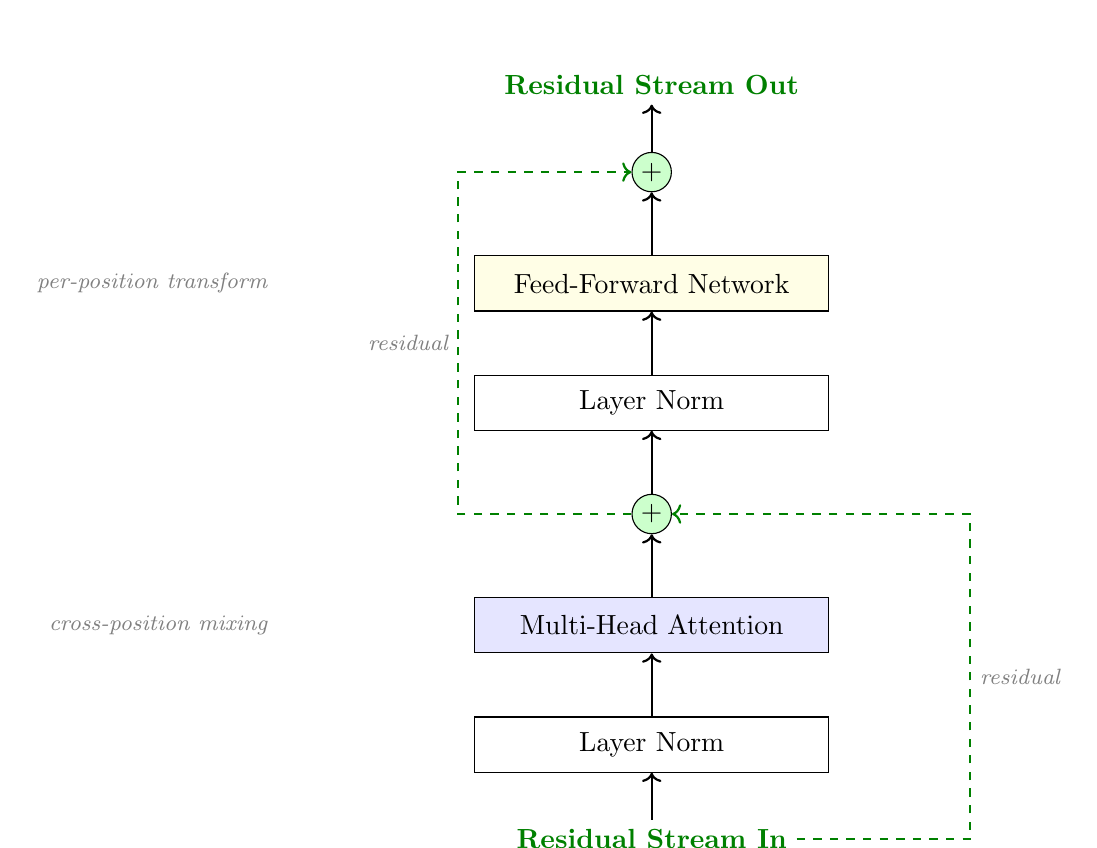
\begin{tikzpicture}[
    node distance=1.0cm,
    block/.style={rectangle, draw, minimum width=4.5cm, minimum height=0.7cm, align=center},
    greenblock/.style={block, fill=green!10},
    blueblock/.style={block, fill=blue!10},
    yellowblock/.style={block, fill=yellow!10},
    addnode/.style={circle, draw, fill=green!20, minimum size=0.5cm, inner sep=0pt},
    arr/.style={->, thick},
    label/.style={font=\footnotesize\itshape, text=gray}
]
    % Bottom: Residual Stream In
    \node[font=\bfseries\color{green!50!black}] (in) {Residual Stream In};
    \node[block, above=0.6cm of in] (ln1) {Layer Norm};
    \node[blueblock, above=0.8cm of ln1] (attn) {Multi-Head Attention};
    \node[addnode, above=0.8cm of attn] (add1) {$+$};
    \node[block, above=0.8cm of add1] (ln2) {Layer Norm};
    \node[yellowblock, above=0.8cm of ln2] (ffn) {Feed-Forward Network};
    \node[addnode, above=0.8cm of ffn] (add2) {$+$};
    \node[font=\bfseries\color{green!50!black}, above=0.6cm of add2] (out) {Residual Stream Out};

    % Arrows
    \draw[arr] (in) -- (ln1);
    \draw[arr] (ln1) -- (attn);
    \draw[arr] (attn) -- (add1);
    \draw[arr] (add1) -- (ln2);
    \draw[arr] (ln2) -- (ffn);
    \draw[arr] (ffn) -- (add2);
    \draw[arr] (add2) -- (out);

    % Residual skip connections
    \draw[arr, dashed, green!50!black] (in.east) -- ++(2.2,0) |- (add1.east) node[pos=0.25, right, label] {residual};
    \draw[arr, dashed, green!50!black] (add1.west) -- ++(-2.2,0) |- (add2.west) node[pos=0.25, left, label] {residual};

    % Side labels
    \node[label, left=2.5cm of attn] {cross-position mixing};
    \node[label, left=2.5cm of ffn] {per-position transform};
\end{tikzpicture}
\caption{A single transformer block. The residual stream (green) flows vertically, carrying each token's representation. Attention and FFN are ``side computations'' that read from the stream and add their results back. This is the highway/off-ramp analogy: the stream is the highway, and each sub-layer is an off-ramp that reads, transforms, and writes back.}
\label{fig:transformer-block}
\end{figure}


\section{Stacking Blocks into a Model}
\label{sec:stacking}

A complete transformer language model stacks $L$ transformer blocks, each with the same architecture but independently learned parameters, on top of each other. The output of block 1's residual stream becomes the input to block 2, and so on. A small model might have $L = 12$ blocks; a large one might have $L = 80$ or more. Figure~\ref{fig:full-model} shows the complete architecture, from input text to output probabilities.

\begin{figure}[ht]
\centering
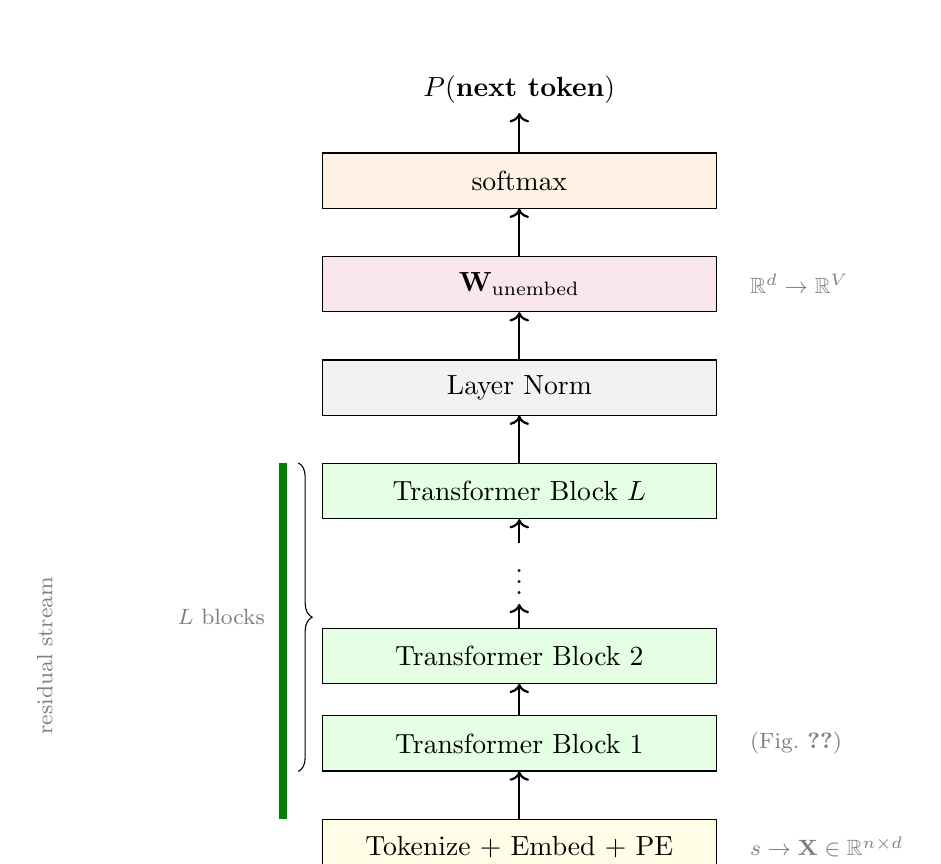
\begin{tikzpicture}[
    node distance=0.8cm,
    block/.style={rectangle, draw, minimum width=5cm, minimum height=0.7cm, align=center},
    greenblock/.style={block, fill=green!10},
    purpleblock/.style={block, fill=purple!10},
    yellowblock/.style={block, fill=yellow!10},
    grayblock/.style={block, fill=gray!10},
    arr/.style={->, thick},
    label/.style={font=\footnotesize, text=gray},
    brace/.style={decorate, decoration={brace, amplitude=5pt, mirror}}
]
    % Bottom: input
    \node[yellowblock] (input) {Tokenize + Embed + PE};
    \node[label, right=0.3cm of input] {$s \to \mathbf{X} \in \mathbb{R}^{n \times d}$};

    \node[greenblock, above=0.6cm of input] (b1) {Transformer Block 1};
    \node[label, right=0.3cm of b1] {(Fig.~\ref{fig:transformer-block})};
    \node[greenblock, above=0.4cm of b1] (b2) {Transformer Block 2};
    \node[above=0.3cm of b2] (dots) {$\vdots$};
    \node[greenblock, above=0.3cm of dots] (bL) {Transformer Block $L$};

    \node[grayblock, above=0.6cm of bL] (ln) {Layer Norm};
    \node[purpleblock, above=0.6cm of ln] (unembed) {$\mathbf{W}_{\text{unembed}}$};
    \node[label, right=0.3cm of unembed] {$\mathbb{R}^d \to \mathbb{R}^V$};
    \node[block, fill=orange!10, above=0.6cm of unembed] (softmax) {softmax};
    \node[font=\bfseries, above=0.5cm of softmax] (pout) {$P(\text{next token})$};

    % Arrows
    \draw[arr] (input) -- (b1);
    \draw[arr] (b1) -- (b2);
    \draw[arr] (b2) -- (dots);
    \draw[arr] (dots) -- (bL);
    \draw[arr] (bL) -- (ln);
    \draw[arr] (ln) -- (unembed);
    \draw[arr] (unembed) -- (softmax);
    \draw[arr] (softmax) -- (pout);

    % Brace for L blocks
    \draw[brace] ([xshift=-0.3cm]b1.south west) -- ([xshift=-0.3cm]bL.north west)
        node[midway, left=0.3cm, label] {$L$ blocks};

    % Residual stream bar
    \draw[green!50!black, line width=3pt] ([xshift=-3cm]input.north) -- ([xshift=-3cm]bL.north);
    \node[label, rotate=90, anchor=south] at ([xshift=-3.3cm]b2.west) {residual stream};
\end{tikzpicture}
\caption{The complete decoder-only transformer. Input text is processed by the input pipeline (Figure~\ref{fig:input-pipeline}) into $\mathbf{X}$, which flows through $L$ stacked transformer blocks (each structured as in Figure~\ref{fig:transformer-block}), a final layer normalization, and the unembedding projection. Softmax converts the logits into a probability distribution over the vocabulary. The green bar marks the residual stream that threads through all blocks.}
\label{fig:full-model}
\end{figure}


\subsection{The Decoder-Only Architecture}
\label{sec:decoder-only}

The original transformer (Vaswani et al., 2017) was designed for machine translation and had two distinct halves:
\begin{itemize}
    \item \textbf{Encoder:} processes the input sentence (e.g., French) using \emph{bidirectional} attention---every token can attend to every other token, both left and right. This produces a rich representation of the input where each token's vector encodes its full context. The encoder has no causal mask.
    \item \textbf{Decoder:} generates the output sentence (e.g., English) one token at a time, left-to-right. It uses \emph{causal} (masked) attention so each output token can only attend to earlier output tokens. Crucially, the decoder also has a second attention layer called \emph{cross-attention} that lets each output token attend to all of the encoder's representations---this is how information flows from the input language to the output language.
\end{itemize}

Despite these different roles, the encoder and decoder are \emph{architecturally almost identical}. Each is a stack of transformer blocks (attention $\to$ LayerNorm $\to$ FFN $\to$ LayerNorm $\to$ residual), with the same Q/K/V projections, the same softmax, the same weighted sum of values. The only structural difference is the \textbf{attention mask}:
\begin{itemize}
    \item \textbf{Encoder}: the full $n \times n$ score matrix is used---every position attends to every other position.
    \item \textbf{Decoder}: the upper triangle of the score matrix is set to $-\infty$ before softmax, so position $i$ can only attend to positions $\leq i$.
\end{itemize}
One bit in the mask configuration turns an encoder block into a decoder block. The names ``encoder'' and ``decoder'' describe different \emph{jobs}, not different architectures: the encoder \emph{reads} (processes a complete input bidirectionally), and the decoder \emph{writes} (generates output left-to-right, informed by the encoder's representation via cross-attention). For translation, you need both: read the full French sentence, then write the English one.

Modern LLMs---GPT, LLaMA, Mistral, DeepSeek---use only the decoder half. This is called the \emph{decoder-only} architecture: a single transformer stack with causal masking, so each token can only attend to earlier tokens. Why drop the encoder?
\begin{enumerate}
    \item \textbf{LLMs are not translating between two languages.} They take a prompt and continue it. The input and output are the \emph{same} sequence in the \emph{same} language, so there is no need for a separate ``reading'' module and a ``writing'' module. A single left-to-right model handles both: it ``reads'' the prompt tokens (they attend to each other via causal attention as it processes them), then seamlessly transitions to ``writing'' new tokens.
    \item \textbf{Causal attention enables autoregressive generation.} Generating token $n{+}1$ requires knowing tokens 1 through $n$. The causal mask ensures this naturally---the model never sees future tokens, so each position's hidden state is a valid context for predicting the next token.
    \item \textbf{Simplicity and scale.} One unified architecture with one type of attention (causal self-attention) is simpler to implement, parallelize, and scale than an encoder-decoder with three types (bidirectional self-attention, causal self-attention, and cross-attention).
\end{enumerate}

In a decoder-only model, the input prompt and the generated output are treated as a single sequence processed left-to-right. The causal mask (Section~\ref{sec:attention-mechanism}) ensures that each token can only attend to tokens at earlier positions. This single-pass, left-to-right design is what makes autoregressive generation possible.

\begin{notebox}
\textbf{Encoder-only models still exist.} BERT (Devlin et al., 2019) is an \emph{encoder-only} transformer: bidirectional attention, no causal mask, no autoregressive generation. It is designed for tasks that require understanding a complete input (classification, named entity recognition, question answering) rather than generating new text. Encoder-decoder models also survive in niches like T5 (Raffel et al., 2020) and machine translation. But for open-ended text generation---the task that defines modern LLMs---decoder-only has become the dominant architecture.
\end{notebox}


\subsection{From Hidden States to Token Predictions}
\label{sec:unembedding}

\marginnote{\emph{Logits}: the raw, unnormalized scores output by the unembedding layer---one per vocabulary token.}%
After the final transformer block, the residual stream for each token contains a $d_{\text{model}}$-dimensional vector that encodes everything the model has computed. But this vector lives in the model's internal representation space---it is not yet a prediction about which word comes next. To turn it into one, a final \emph{linear layer} (called the ``language model head'' or ``unembedding'') projects it into the vocabulary.

\paragraph{Why only the last token?} Each position's hidden state summarizes the information available to it. Because of the causal mask, token 1 has only attended to itself, token 2 has attended to tokens 1--2, and so on. Only the \emph{last} token in the sequence, at position $n$, has attended (directly or through the stacked layers) to every previous token. It is the only position whose hidden state $\mathbf{x}_n^{(L)}$ summarizes the entire input context. Since we want to predict what comes \emph{after} the full prompt, it is the only hidden state we need.\footnote{During training, the model computes predictions at \emph{every} position (predicting each token from its predecessors). But at inference time, we only care about the prediction at position $n$---the next token after the full input.}

\paragraph{What the language head does.} Let $\mathbf{h}_n \equiv \mathbf{x}_n^{(L)} \in \mathbb{R}^{d_{\text{model}}}$ denote this final hidden state. The unembedding projects it from the $d_{\text{model}}$-dimensional internal space into a $V$-dimensional vector---one score per word in the vocabulary:
\begin{equation}
\label{eq:unembedding}
\mathbf{z} = \mathbf{h}_n \mathbf{W}_{\text{unembed}} + \mathbf{b}_{\text{unembed}}
\end{equation}
where $\mathbf{W}_{\text{unembed}} \in \mathbb{R}^{d_{\text{model}} \times V}$ and $\mathbf{z} \in \mathbb{R}^V$ is the \emph{logits} vector---the raw, unnormalized scores, one per vocabulary token. Intuitively, each column of $\mathbf{W}_{\text{unembed}}$ is a ``template vector'' for one vocabulary word. The logit $z_j = \mathbf{h}_n \cdot \mathbf{w}_j$ is a dot product measuring how similar the model's internal summary is to the template for word $j$. Higher similarity means the model thinks word $j$ is a more likely continuation.

\marginnote{\emph{Weight tying}: sharing the same matrix for the embedding lookup and the unembedding projection (transposed).}%
In many models, including LLaMA and GPT-2, the embedding matrix $\mathbf{E}$ and unembedding matrix $\mathbf{W}_{\text{unembed}}$ are \emph{tied}---$\mathbf{W}_{\text{unembed}} = \mathbf{E}^\top$---meaning the same $V \times d_{\text{model}}$ matrix is used for both input embedding lookup and output projection (transposed). This is called \emph{weight tying}.\footnote{Ofir Press and Lior Wolf, ``Using the Output Embedding to Improve Language Models,'' \emph{EACL}, 2017.} The intuition is that the embedding and unembedding perform symmetric jobs: the embedding maps a token ID to a vector that ``means'' that token, and the unembedding maps a hidden state to the token whose meaning vector it most resembles. Using the same vectors for both enforces this symmetry and halves the parameter count for these matrices---for a model with $V = 128{,}000$ and $d_{\text{model}} = 4{,}096$, that saves $V \times d_{\text{model}} \approx 500$M parameters (${\sim}1$\,GB in FP16). Not all models tie weights: GPT-3 and some Mistral variants use separate embedding and unembedding matrices, which allows the output space to be richer at the cost of additional parameters.

These logits are not probabilities yet. A softmax converts them into a probability distribution over the vocabulary:
\begin{equation}
\label{eq:softmax-output}
P(\text{token}_j \mid \text{context}) = \frac{e^{z_j}}{\sum_{\ell=1}^{V} e^{z_\ell}}
\end{equation}
where the denominator sums over all $V$ tokens in the vocabulary, ensuring the probabilities sum to one.

The model's prediction is this probability distribution. The next step---actually choosing a token---is the subject of the next section.


\subsection{A Single Forward Pass (Before Generation)}
\label{sec:forward-pass}

We can now write the full chain from input text to output probability, using every variable introduced in this chapter. Note that this is a \emph{single} forward pass---the model processes the input and produces one probability distribution. How it uses that distribution to generate text, token by token, is the subject of Section~\ref{sec:autoregressive}. A single forward pass through a decoder-only transformer with $L$ layers computes:
\begin{equation}
\label{eq:full-forward}
\begin{aligned}
[t_1, \ldots, t_n] &= \text{Tokenize}(s) & &(\text{string} \to \text{token IDs}) \\
\mathbf{X}^{(0)} &= \mathbf{E}[[t_1, \ldots, t_n]] + \text{PE} & &(\text{embed} + \text{position})
\end{aligned}
\end{equation}

Then for each layer $\ell = 1, \ldots, L$, expand the transformer block explicitly:\footnote{$\text{MultiHead}(\text{LN}(\mathbf{X}))$ is shorthand for the full computation from Equations~\ref{eq:attention}--\ref{eq:multihead}: the layer-normed input is projected by $h$ independent sets of $\mathbf{W}_i^Q, \mathbf{W}_i^K, \mathbf{W}_i^V$ matrices, each head runs the attention mechanism in parallel, the $h$ outputs are concatenated, and $\mathbf{W}^O$ projects the result back to $d_{\text{model}}$. We write it as a single function because the input and output shapes are both $n \times d_{\text{model}}$---the parallelism over heads is internal.}
\begin{align}
\mathbf{A}^{(\ell)} &= \text{MultiHead}\!\Big(\text{LN}\!\big(\mathbf{X}^{(\ell-1)}\big)\Big) & &(\text{attention on layer-normed input}) \notag \\
\mathbf{X}_{\text{mid}}^{(\ell)} &= \mathbf{X}^{(\ell-1)} + \mathbf{A}^{(\ell)} & &(\text{first residual add}) \notag \\
\mathbf{F}^{(\ell)} &= \text{FFN}\!\Big(\text{LN}\!\big(\mathbf{X}_{\text{mid}}^{(\ell)}\big)\Big) & &(\text{feed-forward on layer-normed input}) \notag \\
\mathbf{X}^{(\ell)} &= \mathbf{X}_{\text{mid}}^{(\ell)} + \mathbf{F}^{(\ell)} & &(\text{second residual add})
\end{align}

Finally, extract the last token's hidden state and project to vocabulary. The matrix $\mathbf{X}^{(L)} \in \mathbb{R}^{n \times d_{\text{model}}}$ has one row per token; we take the last row:
\[
\mathbf{X}^{(L)} = \begin{bmatrix} -\;\mathbf{x}_1^{(L)}\;- \\ -\;\mathbf{x}_2^{(L)}\;- \\ \vdots \\ -\;\mathbf{x}_n^{(L)}\;- \end{bmatrix} \in \mathbb{R}^{n \times d_{\text{model}}} \qquad \xrightarrow{\text{extract row } n} \qquad \mathbf{x}_n^{(L)} \in \mathbb{R}^{1 \times d_{\text{model}}}
\]
\[
\mathbf{z} = \mathbf{x}_n^{(L)}\,\mathbf{W}_{\text{unembed}} + \mathbf{b}_{\text{unembed}} \qquad (\text{hidden state} \to \text{logits})
\]
\[
P(\text{token}_j) = \frac{e^{z_j}}{\sum_{\ell=1}^{V} e^{z_\ell}} \qquad (\text{logits} \to \text{probabilities})
\]

Each layer $\ell$ has its own learned parameters ($\mathbf{W}_i^{Q(\ell)}, \mathbf{W}_i^{K(\ell)}, \mathbf{W}_i^{V(\ell)}, \mathbf{W}^{O(\ell)}, \mathbf{W}_1^{(\ell)}, \mathbf{W}_2^{(\ell)}$, and layer norm parameters), all independently trained. The four lines in the middle are exactly the transformer block from Figure~\ref{fig:transformer-block}: layer norm, attention, residual add, layer norm, FFN, residual add. We use $\mathbf{x}_n^{(L)}$---the last token's row of $\mathbf{X}^{(L)}$---because, as explained in Section~\ref{sec:unembedding}, only the last position has attended to the entire input.


\section{Autoregressive Generation}
\label{sec:autoregressive}

\marginnote{\emph{Autoregressive}: each output token depends on all previous tokens, generated one at a time in sequence.}%
A language model does not produce a complete response in one shot. It generates one token at a time. Each newly generated token is appended to the sequence, and the model runs again to produce the next token. This process is called \emph{autoregressive generation}.

\begin{algorithm}
\caption{Autoregressive generation (simplified)}
\label{alg:autoregressive}
\begin{algorithmic}[1]
\Require Prompt tokens $[t_1, t_2, \ldots, t_n]$; model $\mathcal{M}$; max tokens $T$
\Ensure Generated tokens $[t_{n+1}, t_{n+2}, \ldots]$
\State $\text{sequence} \gets [t_1, t_2, \ldots, t_n]$
\For{$i \gets 1$ \textbf{to} $T$}
    \State $\mathbf{z} \gets \mathcal{M}(\text{sequence})$ \Comment{Forward pass through all layers}
    \State $\mathbf{p} \gets \text{softmax}(\mathbf{z}/\tau)$ \Comment{Convert logits to probabilities}
    \State $t_{\text{new}} \gets \text{sample}(\mathbf{p})$ \Comment{Select next token}
    \If{$t_{\text{new}} = EOS$}
        \State \textbf{break}
    \EndIf
    \State Append $t_{\text{new}}$ to sequence
\EndFor
\State \Return generated tokens
\end{algorithmic}
\end{algorithm}

\paragraph{Why not generate all tokens at once?} Algorithm~\ref{alg:autoregressive} reveals a fundamental constraint: generation is inherently sequential. The model cannot produce tokens 5 and 6 simultaneously, because the probability distribution for token 6 depends on which token was actually chosen at position 5. If the sampler picks ``sunny'' for token 5, the distribution for token 6 might peak at ``and'' or ``weather.'' But if the sampler had instead picked ``rainy,'' the distribution for token 6 would be completely different. Each sampling step \emph{collapses} a probability distribution into a single choice, and that choice changes the input for the next step. This is not an engineering limitation---it is a mathematical property of autoregressive factorization: $P(t_1, \ldots, t_n) = \prod_{i=1}^{n} P(t_i \mid t_1, \ldots, t_{i-1})$. Each factor conditions on the \emph{actual} previous tokens, not their probability distributions. Speculative decoding (Section~\ref{sec:distributed:speculative}) partially mitigates this by guessing multiple tokens ahead with a small draft model and verifying them in parallel, but the fundamental sequential dependence remains.

\marginnote{\emph{EOS}: End-Of-Sequence, a special token that signals generation is complete.}%
\paragraph{The EOS token.} The stopping condition in line 6 of Algorithm~\ref{alg:autoregressive} deserves explanation. Every tokenizer includes a special \emph{end-of-sequence} (EOS) token in its vocabulary---a token that never appears in normal text. During training, the model learns that EOS marks the natural end of a response. When the model generates EOS during inference, the system stops decoding immediately: the response is complete. Without EOS, the model would generate text up to the maximum token limit, often producing incoherent trailing output. In practice, chat models use format-specific stop tokens (e.g., \texttt{<|im\_end|>} for ChatML, \texttt{</s>} for LLaMA) that serve the same purpose.


\subsection{Sampling and Temperature}
\label{sec:sampling}

\marginnote{\emph{Temperature} ($\tau$): a parameter that controls the randomness of generation. Lower values make output more deterministic; higher values make it more random.}%
Given the probability distribution over the vocabulary, how do we choose the next token?

\paragraph{Greedy decoding.} Always pick the token with the highest probability. This is deterministic and fast, but tends to produce repetitive, ``safe'' text.

\paragraph{Sampling.} Draw a token randomly from the probability distribution. This introduces diversity but can produce incoherent text if low-probability tokens are chosen.

\paragraph{Temperature.}\footnote{\textbf{Temperature} ($\tau$): a parameter that controls the randomness of generation. Lower values make output more deterministic; higher values make it more random.} Before applying softmax, divide the logits by a \emph{temperature} parameter $\tau > 0$:
\begin{equation}
\label{eq:temperature}
P(\text{token}_j) = \frac{e^{z_j / \tau}}{\sum_{k=1}^{V} e^{z_k / \tau}}
\end{equation}
where $\tau$ is the temperature parameter, $z_j$ is the logit for token $j$, and $V$ is the vocabulary size.

When $\tau = 1$, the distribution is unchanged. When $\tau < 1$ (e.g., 0.3), the distribution becomes sharper---high-probability tokens get even higher probability, and the model behaves more deterministically. When $\tau > 1$, the distribution flattens---low-probability tokens become more likely, and the output becomes more ``creative'' (and potentially less coherent). As $\tau \to 0$, sampling converges to greedy decoding.

\paragraph{Top-\emph{k} and top-\emph{p} sampling.} In practice, sampling is further refined by restricting the candidate set. \emph{Top-$k$} sampling considers only the $k$ highest-probability tokens. \emph{Top-$p$} (nucleus) sampling considers the smallest set of tokens whose cumulative probability exceeds a threshold $p$. Both prevent the model from choosing extremely unlikely tokens while preserving diversity.

% Figure 2.6: Four decoding strategies
\begin{figure}[ht]
\centering
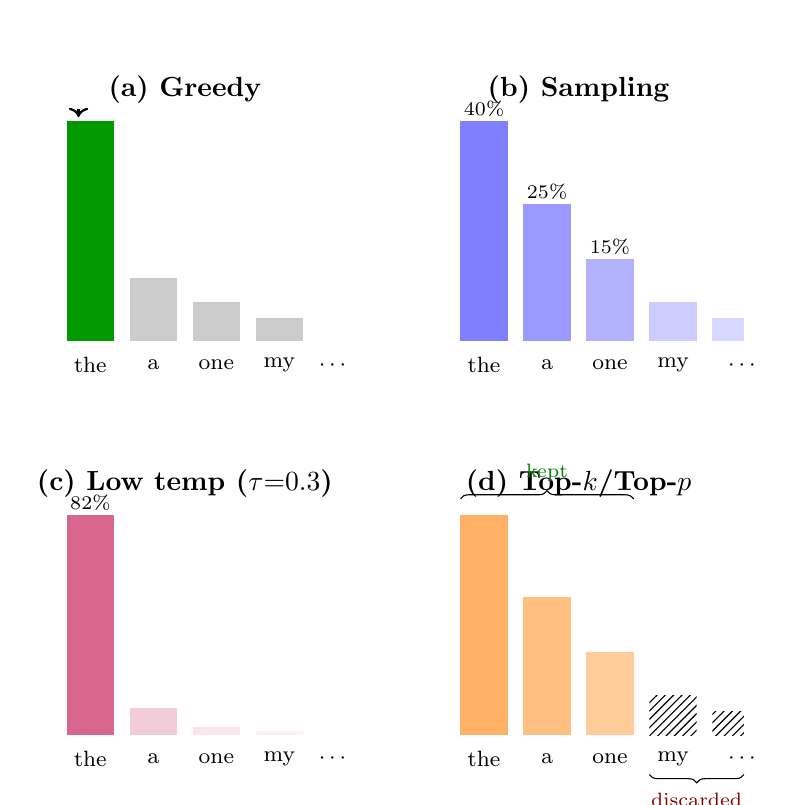
\begin{tikzpicture}
    % (a) Greedy
    \begin{scope}[shift={(0,0)}]
        \node[font=\bfseries] at (1.5,3.2) {(a) Greedy};
        \fill[green!60!black] (0,0) rectangle (0.6,2.8);
        \fill[gray!40] (0.8,0) rectangle (1.4,0.8);
        \fill[gray!40] (1.6,0) rectangle (2.2,0.5);
        \fill[gray!40] (2.4,0) rectangle (3.0,0.3);
        \draw[->, thick] (0.15,2.95) -- (0.15,2.85);
        \node[font=\footnotesize] at (0.3,-0.3) {the};
        \node[font=\footnotesize] at (1.1,-0.3) {a};
        \node[font=\footnotesize] at (1.9,-0.3) {one};
        \node[font=\footnotesize] at (2.7,-0.3) {my};
        \node[font=\footnotesize] at (3.4,-0.3) {$\cdots$};
    \end{scope}
    % (b) Sampling
    \begin{scope}[shift={(5,0)}]
        \node[font=\bfseries] at (1.5,3.2) {(b) Sampling};
        \fill[blue!50] (0,0) rectangle (0.6,2.8);
        \node[font=\scriptsize] at (0.3,2.95) {40\%};
        \fill[blue!40] (0.8,0) rectangle (1.4,1.75);
        \node[font=\scriptsize] at (1.1,1.9) {25\%};
        \fill[blue!30] (1.6,0) rectangle (2.2,1.05);
        \node[font=\scriptsize] at (1.9,1.2) {15\%};
        \fill[blue!20] (2.4,0) rectangle (3.0,0.5);
        \fill[blue!15] (3.2,0) rectangle (3.6,0.3);
        \node[font=\footnotesize] at (0.3,-0.3) {the};
        \node[font=\footnotesize] at (1.1,-0.3) {a};
        \node[font=\footnotesize] at (1.9,-0.3) {one};
        \node[font=\footnotesize] at (2.7,-0.3) {my};
        \node[font=\footnotesize] at (3.6,-0.3) {$\cdots$};
    \end{scope}
    % (c) Low temp
    \begin{scope}[shift={(0,-5)}]
        \node[font=\bfseries] at (1.5,3.2) {(c) Low temp ($\tau{=}0.3$)};
        \fill[purple!60] (0,0) rectangle (0.6,2.8);
        \node[font=\scriptsize] at (0.3,2.95) {82\%};
        \fill[purple!20] (0.8,0) rectangle (1.4,0.35);
        \fill[purple!10] (1.6,0) rectangle (2.2,0.1);
        \fill[purple!5] (2.4,0) rectangle (3.0,0.05);
        \node[font=\footnotesize] at (0.3,-0.3) {the};
        \node[font=\footnotesize] at (1.1,-0.3) {a};
        \node[font=\footnotesize] at (1.9,-0.3) {one};
        \node[font=\footnotesize] at (2.7,-0.3) {my};
        \node[font=\footnotesize] at (3.4,-0.3) {$\cdots$};
    \end{scope}
    % (d) Top-k/Top-p
    \begin{scope}[shift={(5,-5)}]
        \node[font=\bfseries] at (1.5,3.2) {(d) Top-$k$/Top-$p$};
        \fill[orange!60] (0,0) rectangle (0.6,2.8);
        \fill[orange!50] (0.8,0) rectangle (1.4,1.75);
        \fill[orange!40] (1.6,0) rectangle (2.2,1.05);
        \draw[decorate, decoration={brace, amplitude=3pt}] (0,3.0) -- (2.2,3.0) node[midway, above=3pt, font=\scriptsize\color{green!50!black}] {kept};
        \fill[gray!30, pattern=north east lines] (2.4,0) rectangle (3.0,0.5);
        \fill[gray!30, pattern=north east lines] (3.2,0) rectangle (3.6,0.3);
        \draw[decorate, decoration={brace, amplitude=3pt, mirror}] (2.4,-0.5) -- (3.6,-0.5) node[midway, below=3pt, font=\scriptsize\color{red!50!black}] {discarded};
        \node[font=\footnotesize] at (0.3,-0.3) {the};
        \node[font=\footnotesize] at (1.1,-0.3) {a};
        \node[font=\footnotesize] at (1.9,-0.3) {one};
        \node[font=\footnotesize] at (2.7,-0.3) {my};
        \node[font=\footnotesize] at (3.6,-0.3) {$\cdots$};
    \end{scope}
\end{tikzpicture}
\caption{Four decoding strategies applied to the same probability distribution. \textbf{(a)}~Greedy: always pick the maximum. \textbf{(b)}~Sampling: draw from the full distribution. \textbf{(c)}~Low temperature ($\tau = 0.3$): sharpen the distribution before sampling, concentrating mass on the top token. \textbf{(d)}~Top-$k$/top-$p$: discard the tail (hatched bars), renormalize the remaining tokens, then sample. In this example, top-3 and top-$p = 0.8$ select the same set ($0.40 + 0.25 + 0.15 = 0.80$).}
\label{fig:decoding-strategies}
\end{figure}

\begin{insightbox}
From an inference system's perspective, the \emph{sampling strategy does not affect the computational cost}. Whether the system uses greedy decoding or top-$p$ sampling, the model must still compute the full probability distribution over the entire vocabulary for every single generated token. Sampling is a cheap post-processing step; the expensive part is the forward pass.
\end{insightbox}


\section{The Two Phases: Prefill and Decode}
\label{sec:prefill-decode}

We now arrive at the most important concept in this chapter for understanding inference systems. When a user sends a prompt and the model generates a response, the computation falls into two distinct phases with fundamentally different performance characteristics.


\subsection{Prefill: Processing the Prompt}
\label{sec:prefill}

\marginnote{\emph{Compute-bound}: the bottleneck is how fast the GPU can perform arithmetic, not how fast it can read data from memory.}%
The \emph{prefill} phase processes the entire input prompt in a single forward pass. If the user sends a prompt that tokenizes to 1,000 tokens, the model processes all 1,000 tokens at once. This is possible because the prompt is known in advance---there is nothing autoregressive about it.

During prefill, the core operations are \emph{matrix-matrix multiplications}: the $n \times d$ input matrix is multiplied by the $d \times d_k$ projection matrices, the $n \times d_k$ query matrix is multiplied by the $n \times d_k$ key matrix (transposed), and so on. Each of these is a large, dense matrix multiplication.

GPUs are extraordinary at matrix-matrix multiplication. The arithmetic intensity---the ratio of computation (floating-point operations) to memory access (bytes read)---is high. Multiplying an $n \times d$ matrix by a $d \times d_k$ projection matrix involves $O(n \cdot d \cdot d_k)$ floating-point operations but only requires reading $O(n \cdot d + d \cdot d_k)$ bytes. When $n$ is large (a long prompt), the GPU's compute units are fully utilized: every byte fetched from memory is reused many times. This makes prefill \textbf{compute-bound}---the GPU's arithmetic throughput (measured in TFLOPS) is the limiting factor.


\subsection{Decode: Generating Tokens}
\label{sec:decode}

\marginnote{\emph{Memory-bandwidth-bound}: the bottleneck is how fast the GPU can read data from memory, not how fast it can compute.}%
The \emph{decode} phase generates the response one token at a time. At each step, the model processes just the \emph{single} most recently generated token. The core operations become \emph{matrix-vector multiplications}: the single $1 \times d$ token vector is multiplied by each $d \times d_k$ weight matrix.

Here the arithmetic intensity collapses.\footnote{\textbf{Memory-bandwidth-bound}: the bottleneck is how fast the GPU can read data from memory, not how fast it can compute.} Multiplying a $d \times d$ weight matrix by a single vector involves $O(d^2)$ operations---but requires reading all $d^2$ weight entries from memory. Every byte is used only once and then discarded. The GPU's compute units are idle most of the time, waiting for data to arrive from \emph{High-Bandwidth Memory} (HBM).\footnote{\textbf{HBM}: High-Bandwidth Memory, the GPU's main memory. An A100 has 80\,GB of HBM with ${\sim}2$\,TB/s bandwidth.}

This is the fundamental asymmetry of LLM inference:

\begin{insightbox}
\textbf{Prefill is compute-bound; decode is memory-bandwidth-bound.} During prefill, the GPU processes many tokens in parallel and its arithmetic units are the bottleneck. During decode, the GPU processes one token at a time and spends most of its time reading model weights from memory. These two phases have opposite bottlenecks, which is why advanced serving systems (including Dynamo) run them on separate, independently optimized GPU pools---a technique called \emph{disaggregated serving} (Section~\ref{sec:distributed:disaggregated}).
\end{insightbox}

Let us make this concrete with numbers. Consider a model with 70 billion parameters stored in 16-bit floating point (2 bytes each), running on an NVIDIA A100 GPU:
\begin{itemize}
    \item \textbf{Model weights in memory}: $70 \times 10^9 \times 2 = 140$\,GB. This exceeds a single A100's 80\,GB HBM, requiring at least two GPUs for tensor-parallel inference.
\end{itemize}

\begin{notebox}
\textbf{Why ``2 bytes per parameter''?} The $70\text{B} \times 2 = 140$\,GB calculation assumes \emph{FP16} (IEEE 754 half-precision) or \emph{BF16} (bfloat16) storage---both use 16 bits (2 bytes) per floating-point number. During training, models typically use FP32 (4 bytes, 32-bit) for the master copy of weights, but for inference, half-precision is standard because it halves memory consumption and doubles effective memory bandwidth with negligible accuracy loss on well-trained models.

Why is the accuracy loss negligible? FP16 provides ${\sim}3.3$ decimal digits of precision (10 bits of mantissa), which is more than enough to distinguish the learned weight values in a converged model---the meaningful signal in a trained weight typically spans several orders of magnitude more than the FP16 rounding error. BF16 is even coarser (only ${\sim}2.4$ digits, 7 bits of mantissa) but has the same exponent range as FP32, which avoids overflow/underflow issues; it has become the default for LLM inference.

For even more aggressive compression, \emph{quantization} reduces weights to INT8 (1 byte, $4\times$ compression vs.\ FP32) or INT4 (0.5 bytes, $8\times$). These formats introduce measurable but often acceptable accuracy degradation.\footnotemark{} Our 70B model at INT4 would need only ${\sim}35$\,GB---just enough to fit on a single A100.
\end{notebox}
\footnotetext{Tim Dettmers, Mike Lewis, Younes Belkada, and Luke Zettlemoyer, ``LLM.int8(): 8-bit Matrix Multiplication for Transformers at Scale,'' \emph{NeurIPS}, 2022.}

\begin{itemize}
    \item \textbf{Decode step}: Each generated token requires reading most of the model's weights from HBM---once per decode step, because there is only one token's worth of computation to reuse them for. With two A100s in tensor parallelism, each GPU holds ${\sim}70$\,GB of weights and has ${\sim}2$\,TB/s of bandwidth. The time to read those weights is:
    \[
    \frac{70\,\text{GB}}{2{,}000\,\text{GB/s}} = 35\,\text{ms per token} \quad \Longrightarrow \quad \frac{1}{0.035\,\text{s}} \approx 29\,\text{tokens/s}
    \]
    This is a \emph{memory-bandwidth ceiling}: no amount of additional compute power can generate tokens faster than the GPUs can read the weights. In practice, AllReduce communication between the two GPUs adds overhead, bringing realistic single-request decode to roughly 20--25 tokens per second. Batching multiple requests together amortizes the weight-read cost across all of them, significantly improving \emph{aggregate} throughput.

    \item \textbf{Prefill}: With a 1,000-token prompt, the same weight matrices are reused 1,000 times (once per token in the batch), so the arithmetic intensity is ${\sim}1{,}000\times$ higher. The GPU's 312 TFLOPS (A100 FP16) become the bottleneck instead of memory bandwidth.
\end{itemize}


\subsection{Why This Distinction Matters}
\label{sec:why-prefill-decode}

The prefill/decode dichotomy drives nearly every architectural decision in a modern LLM serving system:
\begin{enumerate}
    \item \textbf{Disaggregated serving} (Section~\ref{sec:distributed:disaggregated}): Prefill and decode have different optimal hardware configurations. Prefill benefits from maximum compute throughput; decode benefits from maximum memory bandwidth. Running them on separate GPU pools, each tuned for its workload, improves overall system efficiency.
    \item \textbf{KV caching} (Chapter~\ref{ch:kvcache}): During decode, each new token must attend to all previous tokens' keys and values. Recomputing these from scratch every step would be catastrophically wasteful. Instead, the system \emph{caches} them---but this cache consumes enormous amounts of GPU memory.
    \item \textbf{Continuous batching} (Section~\ref{sec:distributed:batching}): During decode, each request generates one token per step, using very little compute. Batching multiple requests together increases the arithmetic intensity, amortizing the cost of reading weights over multiple tokens.
    \item \textbf{KV-aware routing} (Chapter~\ref{ch:kvrouter}): If a new request shares a prefix with a previous request, the cached key/value vectors from that prefix can be reused---but only if the new request is routed to the same GPU that holds the cache.
\end{enumerate}

Every subsequent chapter in this guide is, in some sense, an answer to the question: \emph{given that decode is memory-bandwidth-bound and the KV cache is enormous, how do we serve LLMs efficiently?}


\subsection{From Prompt to Response: The Full Inference Trace}
\label{sec:inference-trace}

Let us trace the entire inference process---prefill and decode---through the math of this chapter. The model has $L = 32$ layers and the user's prompt is ``The weather today is.''

\paragraph{Prefill: processing the prompt in parallel.}

\begin{enumerate}
    \item \textbf{Tokenize and embed.}
    \[
    [t_1, \ldots, t_4] = [464, 8917, 3063, 318] \quad \Longrightarrow \quad \mathbf{X}^{(0)} = \mathbf{E}[[t_1, \ldots, t_4]] + \text{PE} \;\in\; \mathbb{R}^{4 \times d_{\text{model}}}
    \]
    Each token ID is an index into the embedding table $\mathbf{E}$, which returns a learned $d_{\text{model}}$-dimensional vector---the model's initial representation of that word fragment. Positional encodings stamp each vector with its position in the sequence so the model can distinguish ``The weather'' from ``weather The.'' The result is a $4 \times d_{\text{model}}$ matrix: the model's raw understanding of the prompt, before any cross-token reasoning.

    \item \textbf{Pass through $L = 32$ transformer blocks.} For each layer $\ell = 1, \ldots, 32$, the block expands into seven sub-steps:
    \begin{enumerate}
        \item \textbf{Layer-normalize} the input: \quad $\hat{\mathbf{X}} = \text{LN}\!\big(\mathbf{X}^{(\ell-1)}\big)$

        \emph{Center and scale each token's vector to zero mean and unit variance, keeping activations stable across 32 layers.}

        \item \textbf{Project} to queries, keys, and values for each of the $h$ attention heads:
        \[
        \mathbf{Q}_i = \hat{\mathbf{X}}\,\mathbf{W}_i^Q, \qquad \mathbf{K}_i = \hat{\mathbf{X}}\,\mathbf{W}_i^K, \qquad \mathbf{V}_i = \hat{\mathbf{X}}\,\mathbf{W}_i^V \qquad (i = 1, \ldots, h)
        \]
        \emph{Each head learns its own ``question'' ($\mathbf{Q}_i$: what am I looking for?), ``index card'' ($\mathbf{K}_i$: what do I contain?), and ``content'' ($\mathbf{V}_i$: what do I offer if matched?) from the same input.}

        \item \textbf{Attend} within each head:
        \[
        \text{head}_i = \text{softmax}\!\left(\frac{\mathbf{Q}_i\,\mathbf{K}_i^\top}{\sqrt{d_k}}\right)\mathbf{V}_i
        \]
        \emph{Score every pair of positions by query-key dot product, scale by $\sqrt{d_k}$ to prevent saturation, normalize to attention weights $\boldsymbol{\alpha}_i$ via softmax, then read a weighted combination of values. The causal mask sets future positions to $-\infty$ before softmax so each token only attends to earlier tokens.}

        \item \textbf{Merge} the $h$ heads and project:
        \[
        \mathbf{A}^{(\ell)} = \text{Concat}(\text{head}_1, \ldots, \text{head}_h)\,\mathbf{W}^O
        \]
        \emph{Each head captures a different type of relationship (syntactic, semantic, positional). Concatenate all $h$ perspectives and project back to $d_{\text{model}}$ dimensions with $\mathbf{W}^O$.}

        \item \textbf{First residual add}: \quad $\mathbf{X}_{\text{mid}}^{(\ell)} = \mathbf{X}^{(\ell-1)} + \mathbf{A}^{(\ell)}$

        \emph{Add the gathered context back to the residual stream. The original signal is preserved---the layer only needs to learn the change.}

        \item \textbf{Feed-forward network}: \quad $\mathbf{F}^{(\ell)} = \text{FFN}\!\Big(\text{LN}\!\big(\mathbf{X}_{\text{mid}}^{(\ell)}\big)\Big)$

        \emph{Each token independently passes through two linear layers with a nonlinearity: project up to $4 \times d_{\text{model}}$ dimensions (detect feature combinations), then project back down. This is the model's learned knowledge store---where factual associations live.}

        \item \textbf{Second residual add}: \quad $\mathbf{X}^{(\ell)} = \mathbf{X}_{\text{mid}}^{(\ell)} + \mathbf{F}^{(\ell)}$

        \emph{Add the FFN's output back to the stream. The block is complete; $\mathbf{X}^{(\ell)}$ flows to layer $\ell + 1$.}
    \end{enumerate}

    Each layer's key and value matrices ($\mathbf{K}_i^{(\ell)}, \mathbf{V}_i^{(\ell)}$ for each head $i$) are saved to the \emph{KV cache} (Chapter~\ref{ch:kvcache}). This is the prefill phase: all four tokens are processed in parallel as $4 \times d$ matrix-matrix multiplications. The GPU's compute units are fully utilized.

    \item \textbf{Extract the last token and project to vocabulary.}
    \[
    \mathbf{z} = \mathbf{x}_4^{(32)}\,\mathbf{W}_{\text{unembed}} + \mathbf{b}_{\text{unembed}} \in \mathbb{R}^V \qquad (\text{hidden state} \to \text{per-word score})
    \]
    \[
    P(\text{token}_j) = \frac{e^{z_j / \tau}}{\sum_{k=1}^{V} e^{z_k / \tau}} \qquad (\text{softmax} \to \text{probability distribution})
    \]
    Only the last token (``is'') has attended to the entire prompt through the causal mask (Section~\ref{sec:unembedding}). Its hidden state $\mathbf{x}_4^{(32)}$ summarizes the full context. The unembedding projects this into a score for every word in the vocabulary, softmax converts scores to probabilities, and the sampler selects: token ID $5765 \to$ ``sunny.''
\end{enumerate}

\paragraph{Decode: generating tokens one at a time.} The model now enters the decode loop. The single new token ``sunny'' ($t_5$) is embedded and passed through all 32 layers---but the computation is fundamentally different:
\begin{align}
\mathbf{x}_5^{(0)} &= \mathbf{E}[t_5] + \text{PE}_5 \in \mathbb{R}^{1 \times d_{\text{model}}} & &(\text{embed the single new token}) \notag \\
\mathbf{q}_5^{(\ell)} &= \text{LN}\!\big(\mathbf{x}_5^{(\ell-1)}\big)\,\mathbf{W}^Q \in \mathbb{R}^{1 \times d_k} & &(\textit{one}\text{ query vector, not a matrix}) \notag \\
\mathbf{a}_5^{(\ell)} &= \text{Attention}\!\left(\mathbf{q}_5^{(\ell)},\; \underbrace{\mathbf{K}_{1:5}^{(\ell)}}_{\text{from cache}},\; \underbrace{\mathbf{V}_{1:5}^{(\ell)}}_{\text{from cache}}\right) & &(\text{attend to all 5 tokens via cached K, V}) \notag \\
\mathbf{x}_5^{(\ell)} &= \cdots & &(\text{residual adds and FFN, same as prefill})
\end{align}

The key difference: the model computes a \emph{single} query vector $\mathbf{q}_5$ and dot-products it against the cached keys of all five tokens. This is a matrix-\emph{vector} multiplication, not matrix-matrix. The model reads its full weight set to process one token---most of its time is spent waiting for data from memory, not computing. This is why decode is memory-bandwidth-bound.

After 32 layers, the model extracts $\mathbf{x}_5^{(32)}$, projects to vocabulary, samples the next token, appends a new K/V pair to the cache, and repeats---until an end-of-sequence token is produced or a length limit is reached. Every subsequent decode step is identical: one new token, one query vector, one read of the full weight set.

% Figure 2.7: Prefill vs. Decode comparison
\begin{figure}[ht]
\centering
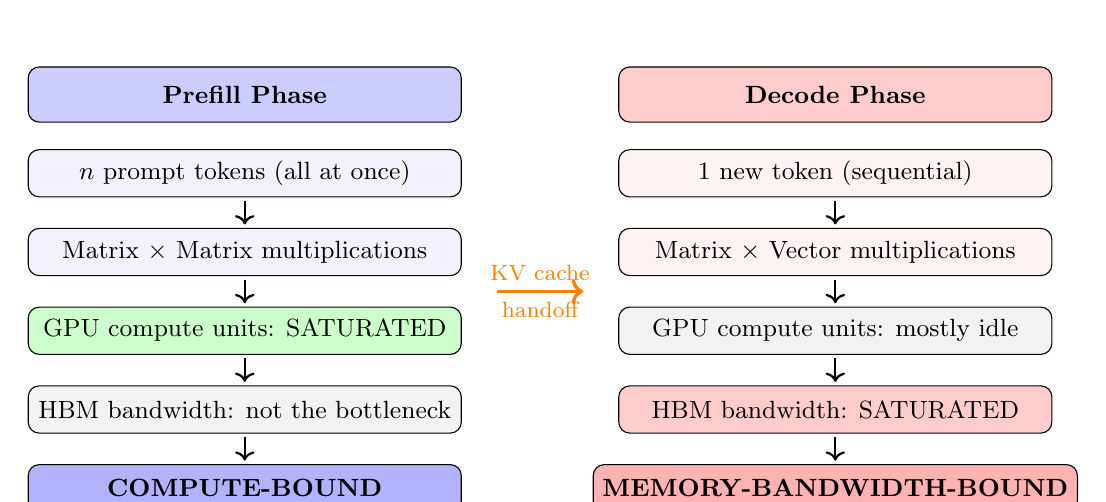
\begin{tikzpicture}[
    phase/.style={rectangle, rounded corners, draw, minimum width=5.5cm, minimum height=0.6cm, align=center, font=\small},
    header/.style={rectangle, rounded corners, draw, fill=#1, minimum width=5.5cm, minimum height=0.7cm, align=center, font=\small\bfseries},
    arr/.style={->, thick},
]
    % Prefill Phase
    \begin{scope}[shift={(0,0)}]
        \node[header=blue!20] (ph) at (0,5) {Prefill Phase};
        \node[phase, fill=blue!5] at (0,4) {$n$ prompt tokens (all at once)};
        \draw[arr] (0,3.65) -- (0,3.35);
        \node[phase, fill=blue!5] at (0,3) {Matrix $\times$ Matrix multiplications};
        \draw[arr] (0,2.65) -- (0,2.35);
        \node[phase, fill=green!20] at (0,2) {GPU compute units: SATURATED};
        \draw[arr] (0,1.65) -- (0,1.35);
        \node[phase, fill=gray!10] at (0,1) {HBM bandwidth: not the bottleneck};
        \draw[arr] (0,0.65) -- (0,0.35);
        \node[phase, fill=blue!30, font=\small\bfseries] at (0,0) {COMPUTE-BOUND};
    \end{scope}

    % Arrow between phases
    \draw[->, very thick, orange] (3.2,2.5) -- (4.3,2.5) node[midway, above, font=\footnotesize] {KV cache} node[midway, below, font=\footnotesize] {handoff};

    % Decode Phase
    \begin{scope}[shift={(7.5,0)}]
        \node[header=red!20] (dh) at (0,5) {Decode Phase};
        \node[phase, fill=red!5] at (0,4) {1 new token (sequential)};
        \draw[arr] (0,3.65) -- (0,3.35);
        \node[phase, fill=red!5] at (0,3) {Matrix $\times$ Vector multiplications};
        \draw[arr] (0,2.65) -- (0,2.35);
        \node[phase, fill=gray!10] at (0,2) {GPU compute units: mostly idle};
        \draw[arr] (0,1.65) -- (0,1.35);
        \node[phase, fill=red!20] at (0,1) {HBM bandwidth: SATURATED};
        \draw[arr] (0,0.65) -- (0,0.35);
        \node[phase, fill=red!30, font=\small\bfseries] at (0,0) {MEMORY-BANDWIDTH-BOUND};
    \end{scope}
\end{tikzpicture}
\caption{Prefill vs.\ Decode: two phases with opposite bottlenecks. Prefill processes all prompt tokens in parallel using matrix-matrix multiplications, saturating the GPU's compute units. Decode generates one token at a time using matrix-vector multiplications, saturating HBM bandwidth. The KV cache (Chapter~\ref{ch:kvcache}) is handed from prefill to decode so that key/value vectors need not be recomputed.}
\label{fig:prefill-vs-decode}
\end{figure}


\section{Summary}
\label{sec:ch2-summary}

We have built the transformer architecture from the ground up:
\begin{itemize}
    \item \textbf{Tokens} are sub-word integer IDs; the \textbf{embedding table} converts them to dense vectors.
    \item The \textbf{attention mechanism} lets each token gather information from other tokens by comparing queries against keys and reading from values. The $\sqrt{d_k}$ scaling prevents softmax saturation.
    \item \textbf{Multi-head attention} runs $h$ parallel attention heads with different learned projections, capturing multiple types of relationships.
    \item A \textbf{transformer block} combines attention (cross-position mixing) and a feed-forward network (per-position transformation), connected by a residual stream with layer normalization.
    \item \textbf{Stacking} $L$ blocks produces a deep model. Decoder-only architectures with causal masking enable left-to-right generation.
    \item \textbf{Autoregressive generation} produces one token at a time, with sampling strategies (temperature, top-$k$, top-$p$) controlling the trade-off between determinism and diversity.
    \item \textbf{Prefill} processes the prompt in parallel and is \textbf{compute-bound}. \textbf{Decode} generates tokens one at a time and is \textbf{memory-bandwidth-bound}. This asymmetry drives the design of every inference serving system.
\end{itemize}

\bigskip
\centerline{\rule{0.3\textwidth}{0.4pt}}
\bigskip

During the decode phase, each new token must attend to every previous token's key and value vectors. But those vectors don't change---recomputing them is pure waste. This observation leads to the single most important data structure in LLM serving.


% ===========================================================================
% Check Your Understanding
% ===========================================================================

\section*{Check Your Understanding}
\addcontentsline{toc}{section}{Check Your Understanding}

\emph{These questions start with recall and progress to conceptual reasoning. All are answerable from this chapter alone.}

\begin{enumerate}
    \item What are the three matrices in the scaled dot-product attention formula, and what role does each play?

    \item In a decoder-only transformer, why can token 5 attend to token 3 but not to token 7?

    \item Why does the attention mechanism divide by $\sqrt{d_k}$?

    \item Explain why the prefill phase is compute-bound and the decode phase is memory-bandwidth-bound. What is fundamentally different about the two computations?

    \item If you removed the residual connections from a transformer, the model would likely fail to train beyond a few layers. Why? What specific problem do residual connections solve, and how does the ``highway'' analogy from this chapter explain it?

    \item The FFN in each transformer block projects from $d_{\text{model}}$ up to $4 \times d_{\text{model}}$ and back down. Attention mixes information \emph{across} token positions, but the FFN operates on each position independently. If the FFN cannot see other tokens, what is it actually contributing to the model's computation? Why is it not redundant with attention?

    \item Suppose someone proposes a ``parallel autoregressive'' scheme: generate all output tokens simultaneously by running the full model once, taking the last-position output as token 1, the second-to-last as token 2, and so on. Explain precisely why this does not work---what mathematical property of the autoregressive factorization $P(t_1, \ldots, t_n) = \prod_i P(t_i \mid t_1, \ldots, t_{i-1})$ is violated, and why each factor's conditioning set matters.

    \item During decode, the model reads its full weight set (140\,GB for a 70B model) to produce a single token. A single A100 has 2\,TB/s of HBM bandwidth. Estimate how many tokens per second a single GPU can generate, and explain why increasing batch size helps---even though each request still needs one token at a time.

    \item The dot product $\mathbf{q}_i \cdot \mathbf{k}_j$ is symmetric: swapping the two vectors gives the same scalar. Yet attention scores are \emph{not} symmetric---token $i$ attending to token $j$ generally produces a different score than token $j$ attending to token $i$. Explain where the asymmetry comes from, and why the transformer's designers chose to keep the symmetric dot product rather than using an inherently asymmetric operator like additive attention.

    \item FlashAttention computes \emph{exactly} the same output as standard attention---it is not an approximation. Yet it reduces memory from $O(n^2)$ to $O(n)$ and runs significantly faster. If the mathematical result is identical, what is actually different? Why does changing the \emph{order} of computation matter so much, and what hardware property makes this possible?

    \item Consider the full inference pipeline: tokenization $\to$ embedding $\to$ $L$ transformer blocks $\to$ unembedding $\to$ softmax $\to$ sampling. Every component except the sampler is deterministic. Yet LLMs produce different responses to the same prompt. Where exactly does randomness enter the system, and why is this randomness \emph{necessary} rather than merely convenient? What would happen to long-form generation if you always picked the highest-probability token?
\end{enumerate}


\subsection*{Answers}

\begin{enumerate}
    \item $\mathbf{Q}$ (queries) represents what each token is looking for; $\mathbf{K}$ (keys) represents what each token advertises about itself; $\mathbf{V}$ (values) represents the information each token provides when attended to. The dot product $\mathbf{Q}\mathbf{K}^\top$ computes relevance scores; softmax normalizes them into weights; the weighted sum over $\mathbf{V}$ extracts the relevant information.

    \item The causal mask. In a decoder-only transformer, future positions are masked to $-\infty$ before softmax, so their attention weights become zero. This enforces the autoregressive property: each token can only depend on tokens at earlier (or equal) positions. Token 5 is at position 5, so it can attend to positions 1--5 but not position 7.

    \item Without scaling, the variance of the dot product $\mathbf{q}_i \cdot \mathbf{k}_j$ grows proportionally to $d_k$ (as shown in the variance derivation). For large $d_k$ (e.g., 128), the dot products become very large in magnitude, pushing softmax into a saturated regime where nearly all probability mass concentrates on one token. In this regime, gradients effectively vanish ($\partial\text{softmax}/\partial z_j \approx 0$), stalling learning. Dividing by $\sqrt{d_k}$ normalizes the variance back to a dimension-independent value, keeping softmax in a responsive range.

    \item \textbf{Prefill}: The model processes $n$ tokens in parallel. The dominant operations are matrix-matrix multiplications ($\mathbf{X}\mathbf{W}^Q$, $\mathbf{Q}\mathbf{K}^\top$, etc.)---large dense operations with high arithmetic intensity (FLOPs per byte of memory accessed). The GPU's compute units are fully utilized. \textbf{Decode}: The model processes one token at a time. The dominant operation is matrix-\emph{vector} multiplication---the full weight matrices must be read from HBM, but each is multiplied by a single vector, so the arithmetic intensity is very low. The GPU spends most of its time waiting for data from memory, not computing. The same weights are read per token either way, but prefill amortizes the read across $n$ tokens.

    \item Residual connections let each layer add its contribution to the residual stream rather than replacing it entirely. Without them, the output of layer $\ell$ \emph{is} the input to layer $\ell + 1$---the entire representation must be reconstructed at every layer. Gradients must propagate through a chain of transformations, vanishing or exploding over many layers. With residual connections, the gradient has a ``skip path'' that flows directly through the addition, keeping it well-behaved. The highway analogy: the residual stream is the highway carrying information from input to output; each layer is an off-ramp that reads from the highway, performs some computation, and adds its result back. If you remove the highway, every layer must perfectly encode \emph{everything} the later layers will need---an impossible burden for early layers.

    \item Attention determines \emph{which} positions are relevant to each other and transfers information between them, but the transferred information is a linear combination of value vectors---attention has no nonlinearity (except softmax, which only affects the \emph{weights}, not the \emph{values}). The FFN provides the model's \emph{nonlinear transformations}: it can detect feature combinations, activate learned knowledge patterns, and compute functions that linear mixing cannot. Think of it as the model's ``knowledge store''---early layers' FFNs learn syntactic patterns, later layers learn factual associations. The two sub-layers are complementary: attention mixes information across positions, and the FFN transforms information within each position.

    \item This fails because each factor $P(t_i \mid t_1, \ldots, t_{i-1})$ in the autoregressive factorization is conditioned on the \emph{actual tokens chosen} at earlier positions, not on a probability distribution over them. When you generate token 6, its distribution depends on which specific token was chosen as token 5. Generating all tokens simultaneously means each position conditions only on the \emph{input prompt}---it has no access to the other generated tokens. This computes $P(t_i \mid \text{prompt})$ independently for each $i$, which is a fundamentally different (and much weaker) distribution. The joint probability $\prod_i P(t_i \mid \text{prompt}) \neq \prod_i P(t_i \mid t_1, \ldots, t_{i-1})$ because the conditioning sets differ. Speculative decoding avoids this problem by having the large model \emph{verify} the draft tokens---it evaluates the true conditional distributions for all draft positions in one forward pass and accepts or rejects each token, preserving the exact autoregressive distribution.

    \item Reading 140\,GB of weights at 2\,TB/s takes $140/2000 = 0.07\,\text{s} = 70\,\text{ms}$ per token, giving roughly $1/0.07 \approx 14$ tokens/s for a single request. With a batch of $B$ requests, the model reads the weights \emph{once} and multiplies them against $B$ query vectors instead of one---the memory read (the bottleneck) is amortized. A batch of 32 produces 32 tokens per weight read, giving ${\sim}450$ tokens/s total throughput at nearly the same per-token latency. Batching converts the operation from matrix-vector (memory-bound) toward matrix-matrix (closer to compute-bound), increasing arithmetic intensity. The limit is GPU memory: the KV cache for all $B$ sequences must also fit in HBM alongside the weights.

    \item The asymmetry comes from the \emph{projections}, not the dot product. When token $i$ attends to token $j$, the model computes $\mathbf{q}_i \cdot \mathbf{k}_j = (\mathbf{x}_i\mathbf{W}^Q) \cdot (\mathbf{x}_j\mathbf{W}^K)$. When token $j$ attends to token $i$, it computes $\mathbf{q}_j \cdot \mathbf{k}_i = (\mathbf{x}_j\mathbf{W}^Q) \cdot (\mathbf{x}_i\mathbf{W}^K)$. These are different computations because the same token gets projected to a different vector depending on its \emph{role}: $\mathbf{x}_i$ becomes $\mathbf{x}_i\mathbf{W}^Q$ when asking but $\mathbf{x}_i\mathbf{W}^K$ when answering, and since $\mathbf{W}^Q \neq \mathbf{W}^K$, these are different vectors. Equivalently, the bilinear form $\mathbf{x}_i\mathbf{M}\mathbf{x}_j^\top$ where $\mathbf{M} = \mathbf{W}^Q{\mathbf{W}^K}^\top$ is not symmetric because $\mathbf{M} \neq \mathbf{M}^\top$ in general. The designers kept the dot product because it can be computed as a single matrix multiplication $\mathbf{Q}\mathbf{K}^\top$---a GEMM that saturates GPU tensor cores (high arithmetic intensity, compute-bound). Additive attention ($\mathbf{w}^\top \tanh(\mathbf{W}_1\mathbf{x}_i + \mathbf{W}_2\mathbf{x}_j)$) is inherently asymmetric but requires $n^2$ element-wise tanh operations that are memory-bandwidth-bound. The design insight: keep the fast symmetric operator and move all asymmetry into the learned projections that feed it.

    \item Standard attention materializes the full $n \times n$ score matrix in HBM (GPU main memory), which requires $O(n^2)$ memory and $O(n^2)$ HBM reads/writes. FlashAttention never materializes this matrix. Instead, it processes the input in blocks that fit in SRAM (the GPU's fast on-chip cache, ${\sim}20$\,MB on an A100 vs.\ 80\,GB of HBM), computing partial softmax results block by block and using the online softmax algorithm to combine them without ever needing the full matrix at once. The mathematical result is identical because online softmax is algebraically exact---it maintains running maximum and sum statistics that it corrects as new blocks arrive. The performance gain comes from the \emph{memory hierarchy}: SRAM is ${\sim}19$\,TB/s vs.\ HBM at ${\sim}2$\,TB/s on an A100. By keeping intermediate data in SRAM and only writing the final output to HBM, FlashAttention reduces HBM accesses from $O(n^2 d_k + n^2)$ to $O(n^2 d_k^2 / M)$ where $M$ is SRAM size. The key hardware property: GPUs have a massive gap between on-chip and off-chip bandwidth, so the order of computation---which data lives where, and for how long---matters enormously even when the total FLOPs are identical.

    \item Randomness enters at exactly one point: the sampling step, after softmax converts logits into a probability distribution. Temperature, top-$k$, and top-$p$ modify this distribution before sampling, but the draw itself is the sole source of non-determinism. This randomness is not just convenient---it is necessary for coherent long-form generation. Greedy decoding (always picking the highest-probability token) is deterministic but produces degenerate output: repetitive loops, generic safe phrasings, and inability to commit to a specific narrative direction. The reason is that the highest-probability token at each step is locally optimal but globally suboptimal---the model may assign 15\% to ``the'' and 12\% to ``a,'' and always choosing ``the'' pushes the model into a narrow corridor of high-frequency text. Sampling allows the model to explore diverse continuations that are collectively more likely under the true distribution than any single greedy path. Temperature controls the exploration-exploitation trade-off: low temperature ($\tau \to 0$) approaches greedy determinism, high temperature ($\tau \to \infty$) approaches uniform randomness. Crucially, sampling does not increase the computational cost at all---the full probability distribution must be computed regardless, and the sampling step itself is negligible.
\end{enumerate}

\chapter{The KV Cache}
\label{ch:kvcache}

The previous chapter showed that every token generated by a transformer requires attending to all previous tokens---computing query-key dot products and value-weighted sums across the entire context. Without intervention, this means re-running the full attention computation from scratch for every single new token. The \emph{KV cache} is the data structure that eliminates this redundancy: it stores the key and value vectors from previous positions so they never need to be recomputed. This chapter explains why the KV cache exists, what it looks like in memory, why it dominates GPU resource consumption, and how two critical innovations---PagedAttention and prefix sharing---make it manageable.

\section{Why Cache?}
\label{sec:kvcache:why}

\marginnote{\emph{Autoregressive generation:} producing one token at a time, each conditioned on all previous tokens.}%
Recall from Chapter~\ref{ch:transformer} that autoregressive generation produces tokens one at a time. At step $t$, the model has already generated positions $1, \ldots, t$ and must compute attention over all of them to produce token $t+1$. The attention mechanism requires key and value vectors for every position in the sequence. The question is: where do those vectors come from?

\subsection{The Na\"ive Approach}

To understand the problem, we need to distinguish two phases of inference. \textbf{Prefill} is the initial phase: the user's entire prompt arrives at once, and the model processes all $n$ prompt tokens in a single parallel forward pass. This is efficient---large batches of matrix multiplications keep the GPU busy. \textbf{Decode} is what comes next: the model generates tokens one at a time, each conditioned on every token before it. Decode is where the waste lives.

Here is why. When the model generates token $t+1$ during decode, it needs to compute attention over positions $1$ through $t$. Attention requires a \emph{key} and \emph{value} vector for every one of those positions (these are the $\mathbf{K}$ and $\mathbf{V}$ matrices from Chapter~\ref{ch:transformer}). Without a cache, the model has no memory of previous steps---so it must recompute every key and value vector from scratch, by re-running the projection $\mathbf{k}_j = \mathbf{W}_K \mathbf{x}_j$ and $\mathbf{v}_j = \mathbf{W}_V \mathbf{x}_j$ for every past position $j$, at every layer. Then for token $t+2$, it does the same thing for positions $1$ through $t+1$---and all the key/value work from the previous step is thrown away and redone.

The waste compounds: position 1's key and value vectors are recomputed at every single decode step. Position 2's vectors are recomputed at every step after the second. And so on. The model is doing the same matrix multiplications over and over, producing the same results each time, because it has nowhere to store them between steps.

Let us quantify the waste. Suppose we start with a prompt of $n$ tokens and want to generate $T$ new tokens. At decode step $i$ (for $i = 1, \ldots, T$), the model must compute key and value projections for all $n + i - 1$ previous positions.\footnote{The projection for position $j$ is $\mathbf{k}_j = \mathbf{W}_K \mathbf{x}_j$ and $\mathbf{v}_j = \mathbf{W}_V \mathbf{x}_j$, each costing $O(d^2)$ operations per layer per head. We absorb the per-element cost into a constant and focus on the scaling in $n$, $T$, and $L$.} The total number of key-value projections across all decode steps is:
\begin{equation}
\label{eq:naive-projections}
\sum_{i=1}^{T} (n + i - 1) = nT + \frac{T(T-1)}{2} = O(nT + T^2)
\end{equation}
Each projection is computed at every layer, so the total work scales as $O\bigl(L \cdot (nT + T^2) \cdot d^2\bigr)$, where $L$ is the number of layers and $d$ is the model dimension. For long generations where $T$ is large, the $T^2$ term dominates---the system does \emph{quadratic} work in the number of generated tokens, not because attention itself is quadratic (that is a separate cost), but because it redundantly recomputes projections.

\subsection{The Caching Insight}

\marginnote{\emph{Immutability:} the key and value vectors for position $j$ depend only on the input at position $j$ and the frozen model weights. They are the same at every decode step.}%
The key observation is simple: the key and value vectors for positions $1, \ldots, t-1$ do not change when we generate token $t$. They depend only on the input at their own position and the (frozen) model weights. We can compute them once, store them, and never recompute them.

With a cache, each decode step computes only the new token's key and value projections---a single row per layer per head---appends them to the stored cache, and performs attention against the full cached sequence. The total number of key-value projections drops from Equation~\ref{eq:naive-projections} to:
\begin{equation}
\label{eq:cached-projections}
n + T
\end{equation}
where $n$ accounts for the initial prompt processing (prefill) and $T$ for the $T$ decode steps, each contributing exactly one new token's projections. Per layer, the projection cost becomes $O\bigl(L \cdot (n + T) \cdot d^2\bigr)$---\emph{linear} in the total sequence length.

\begin{insightbox}
The KV cache trades memory for compute. Without it, each decode step recomputes all keys and values---quadratic total work over a generation. With it, each step computes only the new token's key and value vectors, appends them to the cache, and performs attention against the cached entries. The total projection work drops from $O(nT + T^2)$ to $O(n + T)$ --- a factor-of-$T$ reduction for the projection cost. The attention computation itself ($O(t \cdot d)$ per step, $O(T^2 d / 2)$ total) is inherent and irreducible without approximation; the cache eliminates only the \emph{redundant} projection work, which is the part that was entirely wasted.
\end{insightbox}

\subsection{A Concrete Example}

Consider serving LLaMA-70B with a prompt of $n = 2{,}048$ tokens and a generation length of $T = 512$. Without the cache, Equation~\ref{eq:naive-projections} gives:
\[
2{,}048 \times 512 + \frac{512 \times 511}{2} = 1{,}048{,}576 + 130{,}816 = 1{,}179{,}392 \text{ projection sets}
\]
With the cache, Equation~\ref{eq:cached-projections} gives $2{,}048 + 512 = 2{,}560$ projection sets. The cache reduces the total projection work by a factor of approximately $460 \times$. Each ``projection set'' involves computing a key and value vector across all 80 layers, so the absolute compute savings are enormous: millions of matrix-vector multiplications avoided.

The cost of this saving is memory. Those $2{,}560$ projection sets must be stored somewhere, and as we will see in Section~\ref{sec:kvcache:memory}, for large models this storage dominates GPU memory consumption.

\section{The KV Cache Data Structure}
\label{sec:kvcache:structure}

For each layer $\ell \in \{1, \ldots, L\}$ and each key-value head $h \in \{1, \ldots, H_{\text{KV}}\}$, the KV cache stores two growing tensors:
\begin{align}
\mathbf{K}^{(\ell,h)}_{\text{cache}} &\in \mathbb{R}^{t \times d_k} \\
\mathbf{V}^{(\ell,h)}_{\text{cache}} &\in \mathbb{R}^{t \times d_v}
\end{align}
where $t$ is the current sequence length (which grows by one at each decode step), $d_k$ is the key head dimension, and $d_v$ is the value head dimension (usually $d_k = d_v = d / H$ for the original multi-head attention, but we keep them separate for generality). At each decode step, the new token's key and value vectors are computed and appended as a new row to each cache tensor.

\subsection{Memory Layout}

The full KV cache for a single sequence can be viewed as a 5-dimensional tensor:
\[
\text{Cache} \in \mathbb{R}^{2 \times L \times H_{\text{KV}} \times t \times d_k}
\]
where the leading dimension of 2 accounts for the key and value tensors. In practice, the physical layout varies by implementation:

\begin{itemize}
  \item \textbf{Layer-first layout:} $[L, 2, H_{\text{KV}}, t, d_k]$. Each layer's cache is contiguous, which is natural because attention is computed one layer at a time during the forward pass. This is the layout used by Hugging Face Transformers.
  \item \textbf{Sequence-first layout:} $[2, t, L, H_{\text{KV}}, d_k]$. Each token's full cache across all layers is contiguous, which can improve cache locality for certain memory management strategies.
  \item \textbf{Block layout:} $[2, L, H_{\text{KV}}, \lceil t / B \rceil, B, d_k]$. The sequence dimension is divided into fixed-size blocks of $B$ tokens. This is the layout used by PagedAttention (Section~\ref{sec:kvcache:paged}).
\end{itemize}

\marginnote{\emph{GQA (Grouped-Query Attention):} multiple query heads share a single key-value head, reducing cache size by the group factor $G = H / H_{\text{KV}}$.}%
The crucial parameter is $H_{\text{KV}}$, the number of key-value heads. In the original transformer, every query head has its own key and value head: $H_{\text{KV}} = H$. Modern models use \emph{grouped-query attention} (GQA),\footnote{Joshua Ainslie, James Lee-Thorp, Michiel de Jong, Yinfei Yang, Siddhartha Reddy Jonnalagadda, and Santiago Onta\~{n}\'{o}n, ``GQA: Training Generalized Multi-Query Transformers from Multi-Head Checkpoints,'' \emph{EMNLP}, 2023.} where a group of $G$ query heads shares a single KV head, so $H_{\text{KV}} = H / G$. At the extreme, \emph{multi-query attention} (MQA) uses $H_{\text{KV}} = 1$: all query heads share a single key-value head.

GQA is a direct optimization of cache size. If a model has $H = 64$ query heads but only $H_{\text{KV}} = 8$ KV heads (a group factor of $G = 8$), the KV cache is $8\times$ smaller than it would be with standard multi-head attention. This is not an approximation trick; models are explicitly \emph{trained} with GQA, learning to share KV representations across groups of query heads. LLaMA~2~70B uses $H = 64$ query heads and $H_{\text{KV}} = 8$ GQA heads; LLaMA~3 continues this pattern.

\subsection{Growth Dynamics}

\marginnote{\emph{Prefill:} the initial phase where the entire prompt is processed in one parallel forward pass.\\[4pt]\emph{Decode:} the autoregressive phase where tokens are generated one at a time.}%
During \emph{prefill}, the cache is populated in one shot: the entire prompt of $n$ tokens is processed in parallel, and all $n$ key-value pairs are computed simultaneously at every layer. The cache goes from empty to $t = n$ in a single forward pass.

During \emph{decode}, the cache grows by exactly one row per step. At step $i$, the cache size is $t = n + i$, and the new token's key/value pair is written to position $t$ in each layer's cache. The attention computation reads all $t$ rows to produce the output for the new token.

This asymmetry---bulk write during prefill, incremental append during decode---has profound implications for system design:

\begin{itemize}
  \item \textbf{Prefill is compute-bound.} Processing $n$ tokens in parallel involves large matrix multiplications ($n \times d$ matrices), which saturate the GPU's compute units. The arithmetic intensity (FLOPs per byte of memory accessed) is high.
  \item \textbf{Decode is memory-bound.} Processing 1 token involves reading the entire KV cache ($t$ rows per layer per head) to compute a single dot product per row. The arithmetic intensity is low---most of the time is spent waiting for data to arrive from HBM, not computing.
\end{itemize}

This fundamental asymmetry means that prefill and decode have \emph{opposing} hardware requirements: prefill wants more compute (more FLOPS), while decode wants more memory bandwidth (more HBM bandwidth and capacity). Running both on the same GPU forces a compromise. This is why Dynamo supports \emph{disaggregated serving}: running prefill and decode on separate, independently scaled GPU pools (Chapter~\ref{ch:distributed}). But disaggregation introduces a new problem: after prefill computes the KV cache on a prefill GPU, it must be \emph{transferred} to a decode GPU. The KV cache, which we have just seen can be gigabytes in size, must cross GPU-to-GPU interconnects---making efficient cache transfer and placement a first-class system design concern.

\section{Memory Analysis}
\label{sec:kvcache:memory}

We have seen that the KV cache eliminates redundant computation at the cost of storing every past token's keys and values. How much memory does this actually require? The answer is sobering: the KV cache is the dominant consumer of GPU memory during inference, often exceeding the model weights themselves for large batches with long sequences. Let us build up the calculation from first principles.

\subsection{Per-Token Cache Size}

For a single token at a single layer and a single KV head, the cache stores one key vector ($d_k$ elements) and one value vector ($d_v$ elements). With $d_k = d_v = d_{\text{head}}$ and using $b$ bytes per element (e.g., $b = 2$ for FP16, $b = 1$ for INT8):
\begin{equation}
\label{eq:per-token-per-layer-per-head}
\text{Bytes per token per layer per head} = 2 \times d_{\text{head}} \times b
\end{equation}
Summing across all $H_{\text{KV}}$ heads and $L$ layers:
\begin{equation}
\label{eq:per-token}
\text{Bytes per token} = 2 \times L \times H_{\text{KV}} \times d_{\text{head}} \times b
\end{equation}

\begin{notebox}
\textbf{KV cache size for LLaMA-70B.} With $L = 80$ layers, $H_{\text{KV}} = 8$ GQA heads, $d_{\text{head}} = 128$, and FP16 ($b = 2$ bytes per element):
\[
\text{Cache per token} = 2 \times 80 \times 8 \times 128 \times 2 = 327{,}680\;\text{bytes} \approx 320\;\text{KB}
\]
Every single token in every active sequence consumes 320\,KB of GPU memory just for its cached keys and values. For context, this is larger than the entire L1 cache on most CPUs.
\end{notebox}

Contrast this with a smaller model. For LLaMA-7B ($L = 32$, $H_{\text{KV}} = 32$ with standard MHA, $d_{\text{head}} = 128$, FP16):
\[
\text{Cache per token} = 2 \times 32 \times 32 \times 128 \times 2 = 524{,}288\;\text{bytes} \approx 512\;\text{KB}
\]
The 7B model actually has a \emph{larger} per-token cache than the 70B model because it uses standard multi-head attention ($H_{\text{KV}} = 32$) rather than GQA ($H_{\text{KV}} = 8$). This illustrates why GQA was adopted: it reduces cache size by the group factor without proportional loss in model quality.

\subsection{Batch-Level Memory}

\marginnote{\emph{Batch size:} the number of sequences being processed concurrently. Larger batches amortize the cost of loading model weights but require proportionally more KV cache memory.}%
For a batch of $B$ sequences, each of length $s$ (including both prompt and generated tokens so far):
\begin{equation}
\label{eq:batch-cache}
\text{Total cache memory} = B \times s \times 2 \times L \times H_{\text{KV}} \times d_{\text{head}} \times b
\end{equation}

\begin{notebox}
\textbf{Concrete scenario: LLaMA-70B on an A100-80GB.} The model weights in FP16 occupy approximately 140\,GB, requiring at least 2 A100-80GB GPUs with tensor parallelism. Suppose we split across 2 GPUs, so each GPU holds about 70\,GB of weights. That leaves roughly 10\,GB per GPU for the KV cache.\footnote{In practice, the CUDA runtime, activation memory, and other overheads consume additional memory, leaving less than 10\,GB.}

With 320\,KB per token, 10\,GB supports:
\[
\frac{10 \times 1024^3}{320 \times 1024} \approx 32{,}768 \text{ token-slots}
\]
If each sequence uses up to 4,096 tokens, we can serve at most $32{,}768 / 4{,}096 = 8$ concurrent sequences per GPU. With 2,048-token sequences, we get 16. These are small batches---and batch size directly determines throughput, because larger batches amortize the cost of loading model weights from HBM.
\end{notebox}

This reveals the fundamental tension: \textbf{throughput requires large batches, but large batches require large KV caches, and GPU memory is fixed.} A system that cannot manage cache memory efficiently will either reject requests (reducing throughput) or run out of memory and crash. This is the problem that PagedAttention solves.

\begin{whynotbox}{Why not just add more GPU memory?}
A natural reaction to the KV cache memory problem is: buy bigger GPUs. If 80\,GB is not enough, wait for 160\,GB or 320\,GB parts. This does not solve the problem---it merely shifts the bottleneck.

\textbf{Memory grows linearly; demand grows combinatorially.} Doubling HBM capacity lets you double the batch size \emph{or} double the sequence length---but real workloads want both. A model serving 128K-token contexts at batch size 64 needs $128{,}000 \times 64 \times 320\;\text{KB} \approx 2.5$\,TB of cache for LLaMA-70B. No single GPU comes close.

\textbf{Cost.} HBM is the most expensive component on a GPU die. The A100-80GB costs roughly 2$\times$ the A100-40GB, and the H100-141GB is priced accordingly. Doubling memory to double batch size is a poor trade-off when software can achieve a 2--5$\times$ improvement through better allocation (PagedAttention) at zero hardware cost.

\textbf{Bandwidth, not just capacity.} Even if a GPU had unlimited memory, the decode phase is bottlenecked by \emph{memory bandwidth}---how fast data can be read from HBM, not how much HBM exists. Adding capacity without proportionally increasing bandwidth yields diminishing returns.

The right approach is to use the memory you have more efficiently. That is precisely what PagedAttention and prefix sharing accomplish.
\end{whynotbox}

\subsection{KV Cache vs.\ Model Weights}

For a single short request, the KV cache is much smaller than the model weights. But at batch scale, the cache grows while the weights stay constant:
\begin{center}
\begin{tabular}{lrr}
\hline
\textbf{Component} & \textbf{LLaMA-7B (FP16)} & \textbf{LLaMA-70B (FP16)} \\
\hline
Model weights & 14 GB & 140 GB \\
KV cache (1 seq, 2K tokens) & 1.0 GB & 0.625 GB \\
KV cache (1 seq, 4K tokens) & 2.0 GB & 1.25 GB \\
KV cache (32 seq, 4K tokens) & 64 GB & 40 GB \\
KV cache (64 seq, 4K tokens) & 128 GB & 80 GB \\
\hline
\end{tabular}
\end{center}

At a batch size of 32 with 4K-token sequences, the KV cache for LLaMA-7B ($\sim$64\,GB) is over $4\times$ the model weights (14\,GB). For LLaMA-70B, the 40\,GB cache is a smaller fraction of the 140\,GB weights, but still represents an enormous memory demand that must be carefully managed.

Two trends in model design work in opposite directions. \textbf{GQA reduces cache pressure}: by sharing KV heads across groups of query heads, GQA cuts the per-token cache cost proportionally. LLaMA-70B's use of 8 KV heads instead of 64 reduces its per-token cache from $\sim$2.6\,MB (if it used standard MHA) to $\sim$320\,KB---an $8\times$ reduction. \textbf{Longer context windows increase cache pressure}: extending the maximum context from 4K to 128K tokens multiplies the worst-case cache size by $32\times$. Models like LLaMA~3 support 128K-token contexts, meaning a single sequence could consume $128{,}000 \times 320\;\text{KB} \approx 40$\,GB of cache---more than the entire HBM of many GPUs. These opposing forces make KV cache management one of the most active areas of systems research in LLM inference.

\begin{insightbox}
The KV cache is the reason batch size is limited by GPU memory, not by model weights. Model weights are a fixed cost; the KV cache scales linearly with both the number of concurrent sequences and their lengths. Any system that wants to maximize throughput must minimize KV cache waste---and the dominant source of waste, before PagedAttention, was memory fragmentation from na\"ive allocation strategies.
\end{insightbox}

\section{PagedAttention}
\label{sec:kvcache:paged}

\marginnote{\emph{PagedAttention:} applies OS-style virtual memory paging to KV cache management, eliminating fragmentation. Introduced in the vLLM paper by Kwon et al., 2023.}%
Having established that the KV cache dominates GPU memory and that its size grows linearly with batch size and sequence length, we now turn to the question of \emph{how} that memory is managed. The na\"{\i}ve approach wastes most of it. PagedAttention reclaims that waste.

Traditional KV cache implementations pre-allocate a contiguous block of memory for each sequence at its maximum possible length. If the system's maximum sequence length is 4,096 tokens, every incoming request reserves $4{,}096 \times 320$\,KB $= 1.28$\,GB of cache memory (for LLaMA-70B)---even if the actual generation produces only 50 tokens. The waste is severe: Kwon et al.\footnote{Woosuk Kwon, Zhuohan Li, Siyuan Zhuang, Ying Sheng, Lianmin Zheng, Cody Hao Yu, Joseph E.\ Gonzalez, Hao Zhang, and Ion Stoica, ``Efficient Memory Management for Large Language Model Serving with PagedAttention,'' \emph{SOSP}, 2023.} measured that existing systems waste 60--80\% of KV cache memory due to three forms of fragmentation:

\marginnote{\emph{Fragmentation:} wasted memory due to allocation policies---space that is allocated but unused (internal) or free but unusable (external).}%
\begin{enumerate}
  \item \textbf{Reservation waste.} Space is reserved for the maximum sequence length but most sequences are shorter. A 50-token response in a 4,096-token slot wastes 98.8\% of its allocation.
  \item \textbf{Internal fragmentation.} Even for completed sequences, the allocated buffer may be larger than the final sequence length due to alignment or allocation granularity.
  \item \textbf{External fragmentation.} As sequences arrive and depart at different times, the free memory becomes scattered into non-contiguous chunks, each too small to serve a new request even though the total free memory is sufficient.
\end{enumerate}

\subsection{The Paging Analogy}

PagedAttention applies the same insight that operating systems use for virtual memory: \textbf{decouple the logical layout from the physical layout}. Instead of allocating one contiguous block per sequence, PagedAttention divides GPU memory into fixed-size \emph{pages} (called \emph{blocks} in vLLM's terminology),\footnote{We use ``block'' and ``page'' interchangeably in this chapter. vLLM's codebase uses ``block''; the conceptual analogy is to OS pages.} each holding the keys and values for a fixed number of tokens.

\begin{notebox}
\textbf{Block size.} A typical block size is $B = 16$ tokens. For LLaMA-70B in FP16, one block stores:
\[
16 \times 320\;\text{KB} = 5{,}120\;\text{KB} = 5\;\text{MB}
\]
per layer-head slice. The total block size across all layers and heads is 5\,MB. A single A100-80GB can hold roughly $80{,}000 / 5 \approx 16{,}000$ blocks (in the memory left after model weights), tracking them via a simple free list.
\end{notebox}

\begin{whynotbox}{Why fixed-size blocks instead of variable-size allocations?}
Operating systems faced this same design choice decades ago. Early memory allocators used variable-size allocations, which leads to \emph{external fragmentation}: after many allocations and frees, memory is littered with differently-sized holes, and a request for $N$ bytes can fail even when the total free memory exceeds $N$.

Fixed-size blocks eliminate external fragmentation entirely. Any freed block can satisfy any allocation request---there is no need to search for a ``big enough'' hole or compact memory. The trade-off is \emph{internal fragmentation}: the last block of a sequence is typically partially filled. With block size $B = 16$, the expected waste is $B/2 = 8$ tokens per sequence, which for LLaMA-70B amounts to $8 \times 320\;\text{KB} = 2.5$\,MB---negligible compared to the tens of gigabytes that reservation-based allocation wastes.

A variable-size scheme could waste zero bytes at the tail, but would reintroduce the fragmentation nightmare that makes batch scheduling unpredictable. Fixed blocks give the allocator $O(1)$ allocation and deallocation (just push/pop from a free list), which matters when the scheduler must make allocation decisions on the critical path of every decode step.
\end{whynotbox}

Each sequence maintains a \emph{block table}: an array of pointers mapping logical block indices to physical block addresses. Position $j$ in the sequence maps to logical block $\lfloor j / B \rfloor$, offset $j \bmod B$ within that block. As the sequence grows during decode, new physical blocks are allocated from a shared pool on demand---only when the current block is full and a new token needs space.

\subsection{How It Works}

Consider a sequence that has generated 35 tokens with a block size of 16:
\begin{itemize}
  \item Logical block 0 maps to physical block 7 (tokens 0--15, full)
  \item Logical block 1 maps to physical block 42 (tokens 16--31, full)
  \item Logical block 2 maps to physical block 3 (tokens 32--34, partially filled)
\end{itemize}
Physical blocks 7, 42, and 3 are not contiguous in GPU memory---they could be anywhere. The block table provides the indirection. When token 36 arrives, it is appended to physical block 3 at offset 3. When physical block 3 becomes full (at token 47), a new physical block is allocated from the free pool for logical block 3.

\begin{figure}[ht]
\centering
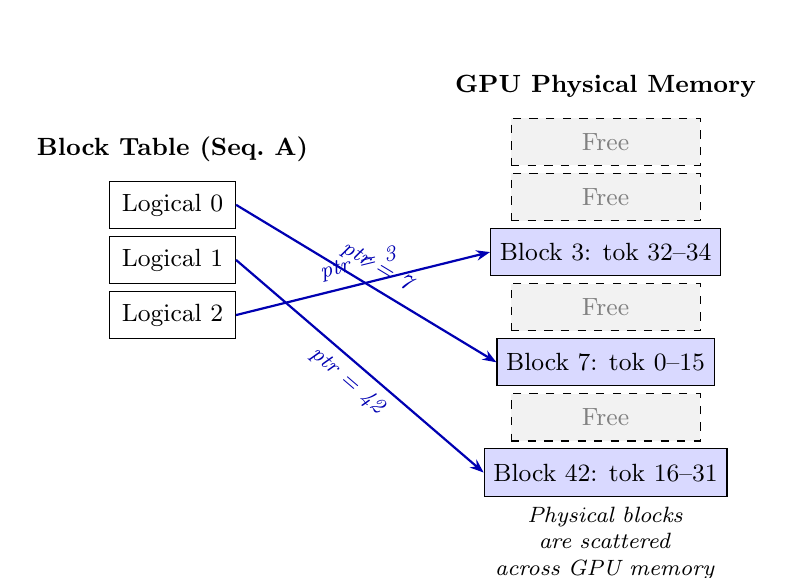
\begin{tikzpicture}[
    blocktable/.style={rectangle, draw, minimum width=1.6cm, minimum height=0.6cm, align=center, font=\small},
    physblock/.style={rectangle, draw, minimum width=2.4cm, minimum height=0.6cm, align=center, font=\small},
    fullblock/.style={physblock, fill=blue!15},
    partialblock/.style={physblock, fill=blue!8, pattern=north east lines, pattern color=blue!15},
    freeblock/.style={physblock, fill=gray!10, dashed},
    arrow/.style={-{Stealth[length=5pt]}, thick},
    label/.style={font=\footnotesize\itshape},
]
    % Block table (left side)
    \node[font=\small\bfseries] at (0, 2.2) {Block Table (Seq.\ A)};
    \node[blocktable] (bt0) at (0, 1.5) {Logical 0};
    \node[blocktable] (bt1) at (0, 0.8) {Logical 1};
    \node[blocktable] (bt2) at (0, 0.1) {Logical 2};

    % Physical memory (right side) -- scattered
    \node[font=\small\bfseries] at (5.5, 3.0) {GPU Physical Memory};

    \node[freeblock] (p0) at (5.5, 2.3) {\textcolor{gray}{Free}};
    \node[freeblock] (p1) at (5.5, 1.6) {\textcolor{gray}{Free}};
    \node[fullblock]  (p3) at (5.5, 0.9) {Block 3: tok 32--34};
    \node[freeblock] (p4) at (5.5, 0.2) {\textcolor{gray}{Free}};
    \node[fullblock]  (p7) at (5.5, -0.5) {Block 7: tok 0--15};
    \node[freeblock] (p8) at (5.5, -1.2) {\textcolor{gray}{Free}};
    \node[fullblock] (p42) at (5.5, -1.9) {Block 42: tok 16--31};

    % Arrows from block table to physical blocks
    \draw[arrow, blue!70!black] (bt0.east) -- (p7.west) node[label, above, midway, sloped] {ptr = 7};
    \draw[arrow, blue!70!black] (bt1.east) -- (p42.west) node[label, below, midway, sloped] {ptr = 42};
    \draw[arrow, blue!70!black] (bt2.east) -- (p3.west) node[label, above, midway, sloped] {ptr = 3};

    % Annotation
    \node[label, text width=3.2cm, align=center] at (5.5, -2.8) {Physical blocks are scattered\\across GPU memory};
\end{tikzpicture}
\caption{PagedAttention block table for a sequence of 35 tokens with block size 16. The block table maps logical block indices to physical block addresses. Physical blocks need not be contiguous---the indirection layer decouples logical sequence order from physical memory layout, exactly as a page table does in an operating system.}
\label{fig:block-table}
\end{figure}

When the sequence finishes (e.g., the model generates an end-of-sequence token), all its physical blocks are returned to the free pool. Because blocks are fixed-size, any freed block can immediately serve any new sequence---there is no external fragmentation. And because blocks are allocated on demand rather than reserved up front, there is no reservation waste.

\subsection{The Block Table}

\marginnote{\emph{Block table:} a per-sequence array mapping logical block indices to physical block addresses in GPU memory---analogous to a page table in an OS.}%
The block table is the central bookkeeping structure. For each active sequence, the system maintains an array:
\[
\text{block\_table}[i] = \text{physical block index for logical block } i
\]
To access the KV cache for token at position $j$:
\begin{enumerate}
  \item Compute the logical block index: $\lfloor j / B \rfloor$
  \item Look up the physical block: $\text{block\_table}[\lfloor j / B \rfloor]$
  \item Compute the offset within the block: $j \bmod B$
  \item Read or write at that offset in the physical block
\end{enumerate}

The block table itself is small---a sequence of 4,096 tokens with block size 16 needs only $4{,}096 / 16 = 256$ entries, each a 32-bit pointer. The total block table overhead across hundreds of concurrent sequences is negligible compared to the cache data itself.

\marginnote{\emph{Reference counting:} tracking how many sequences point to each physical block. A block is freed only when its count reaches zero.}%
When a sequence finishes, its entire block table is scanned and each physical block's reference count is decremented. Blocks with a reference count of zero are returned to the free pool. This deallocation is $O(s / B)$ per sequence---typically a few hundred operations at most.

\subsection{Modified Attention Kernel}

The attention kernel must be modified to follow block table pointers instead of assuming contiguous memory. For each query position, the kernel iterates over the sequence's block table, fetches the key and value data from the indicated physical block, and performs the dot product and weighted sum. The mathematical computation is identical to standard attention---the outputs are bit-for-bit the same. PagedAttention is purely a memory management optimization, not an approximation.

The kernel modification introduces one additional memory indirection per block (reading the block table entry before reading the KV data), but this cost is negligible: the block table is small enough to fit in GPU L2 cache, while the actual KV data dominates the memory access time. In practice, the throughput improvement from higher batch sizes (enabled by reduced waste) far outweighs the minor overhead of the indirection.

\begin{insightbox}
PagedAttention is to GPU memory what virtual memory is to RAM. Just as an OS lets processes see contiguous address spaces backed by scattered physical pages, PagedAttention lets sequences see contiguous KV caches backed by scattered GPU memory blocks. The result is near-zero waste: memory utilization jumps from 20--40\% to over 95\%. This increase in utilization translates directly to higher batch sizes and therefore higher throughput.
\end{insightbox}

\subsection{Quantifying the Improvement}

The impact on serving throughput is dramatic. Consider an A100-80GB serving LLaMA-70B (in a tensor-parallel setup where roughly 10\,GB per GPU is available for the KV cache):

\begin{center}
\begin{tabular}{lrr}
\hline
\textbf{Metric} & \textbf{Without paging} & \textbf{With PagedAttention} \\
\hline
Memory utilization & $\sim$20--40\% & $>$95\% \\
Effective cache capacity & 2--4 GB & 9.5+ GB \\
Max concurrent seqs (4K tokens) & 2--3 & 7--8 \\
Max concurrent seqs (512 tokens) & 6--12 & 59+ \\
\hline
\end{tabular}
\end{center}

For short sequences, the improvement is even more pronounced because the reservation waste under the na\"ive scheme is proportionally larger: a 512-token sequence in a 4,096-token slot wastes 87.5\% of its allocation. PagedAttention reclaims essentially all of that waste.

\subsection{KV Cache Quantization}

\marginnote{\emph{Quantization:} representing values with fewer bits, trading precision for reduced memory and bandwidth.}%
An orthogonal technique for reducing KV cache memory is \emph{quantization}: storing keys and values in lower precision than the model's native format. While the model may compute in FP16 or BF16 (2 bytes per element), the cached keys and values can be quantized to INT8 (1 byte) or even INT4 (0.5 bytes) with minimal impact on output quality.

For LLaMA-70B, moving from FP16 to INT8 halves the per-token cache cost from 320\,KB to 160\,KB. Combined with PagedAttention, this doubles the effective batch size yet again. The trade-off is that quantization introduces small numerical errors in the attention computation---unlike PagedAttention, it is an approximation. However, because keys and values are used only in dot products and weighted sums (not in the more numerically sensitive softmax normalization), the impact on generation quality is typically small. KV cache quantization is supported by most modern inference engines and can be combined with both PagedAttention and prefix sharing.

\section{Prefix Sharing}
\label{sec:kvcache:prefix}

\marginnote{\emph{Prefix sharing:} reusing cached KV blocks across requests that share a common prompt prefix, avoiding redundant computation and storage.}%
PagedAttention eliminates waste \emph{within} a single sequence's allocation. But there is a second, equally large source of waste: \emph{duplication across sequences}. Many production LLM workloads share common prefixes. A system prompt (``You are a helpful assistant\ldots'') may be prepended to every user request. In a coding assistant, the same file context is sent with every completion request. A retrieval-augmented generation (RAG) pipeline may prepend the same set of retrieved documents to multiple queries. Without prefix sharing, each request independently computes and stores KV cache entries for the shared prefix---duplicating both compute and memory.

\subsection{The Opportunity}

Suppose a system prompt of 500 tokens is prepended to every user request. In a batch of 32 concurrent requests, the na\"ive approach stores 32 copies of the same 500-token KV cache---wasting $31 \times 500 \times 320\;\text{KB} \approx 4.8$\,GB for LLaMA-70B. Prefix sharing stores the system prompt's KV cache \emph{once} and lets all 32 sequences reference the same physical blocks:
\begin{equation}
\text{Savings} = (B - 1) \times n_{\text{prefix}} \times c_{\text{token}}
\end{equation}
where $B$ is the batch size, $n_{\text{prefix}}$ is the shared prefix length, and $c_{\text{token}}$ is the per-token cache cost. For our example: $(32 - 1) \times 500 \times 320\;\text{KB} = 4.8$\,GB saved. This is nearly half of the available 10\,GB cache budget, freeing space for additional concurrent requests.

The compute savings are equally significant. Instead of running prefill for the 500-token system prompt 32 times, the system runs it once and reuses the cached keys and values. For a model like LLaMA-70B, prefilling 500 tokens involves roughly $500 \times 2 \times 80 \times 8192^2 \approx 5.4 \times 10^{13}$ FLOPs (considering attention and MLP computations across all layers). Doing this once instead of 32 times saves over $1.6 \times 10^{15}$ FLOPs---multiple seconds of A100 compute time.

\subsection{Mechanism: Block Hashing and Reference Counting}

Prefix sharing requires two capabilities:
\begin{enumerate}
  \item A way to \textbf{identify} whether a given token sequence's KV cache already exists somewhere.
  \item A way to \textbf{share} physical blocks across sequences without copying.
\end{enumerate}

\textbf{Identification via hashing.}\hspace{1em} Token sequences are divided into fixed-size blocks (the same blocks used by PagedAttention), and each block is hashed. In Dynamo, this hashing is performed by the \texttt{dynamo\_tokens} library (Chapter~\ref{ch:tokens}), which computes XXH3 hashes of token blocks:\footnote{XXH3 is a non-cryptographic hash function optimized for speed, producing 64-bit hashes. It runs at over 30\,GB/s on modern CPUs.}
\begin{itemize}
  \item A \emph{local block hash} is computed from the tokens within a single block.
  \item A \emph{sequence hash} chains the local block hash with the previous block's sequence hash, producing a rolling hash that captures the entire prefix up to and including the current block.
\end{itemize}
The sequence hash is critical: two blocks with identical tokens but different preceding contexts will produce different sequence hashes, correctly distinguishing ``\texttt{The cat sat}'' at the start of a prompt from ``\texttt{The cat sat}'' appearing later after different context.

\textbf{Sharing via block pointers.}\hspace{1em} Because PagedAttention already uses block tables with pointers to physical blocks (not contiguous memory), sharing blocks across sequences is straightforward: two sequences' block tables simply point to the same physical blocks for their shared prefix. Reference counting tracks how many sequences use each block. When the last sequence using a shared block finishes, the reference count drops to zero and the block is returned to the free pool.

\begin{figure}[ht]
\centering
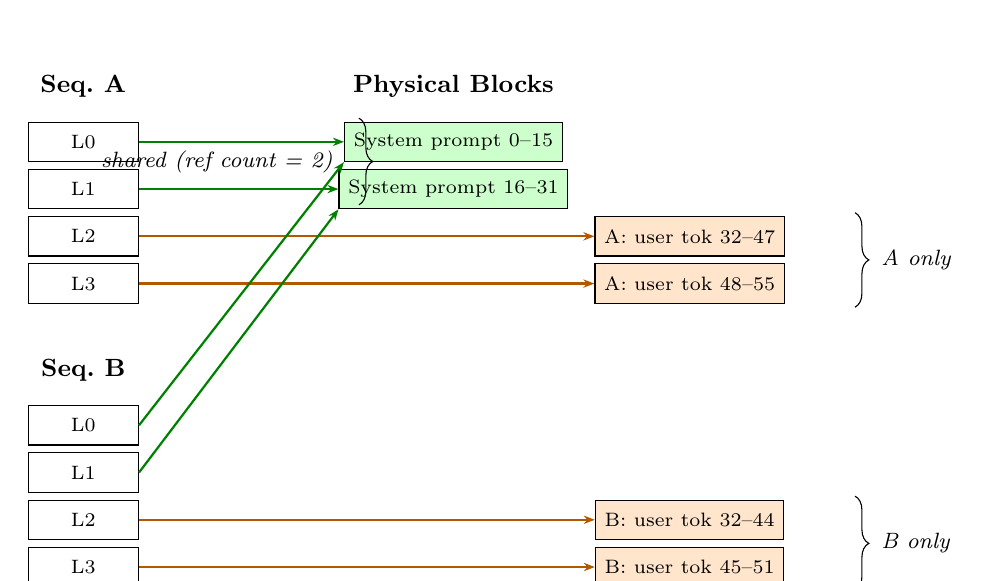
\begin{tikzpicture}[
    blocktable/.style={rectangle, draw, minimum width=1.4cm, minimum height=0.5cm, align=center, font=\scriptsize},
    physblock/.style={rectangle, draw, minimum width=1.8cm, minimum height=0.5cm, align=center, font=\scriptsize},
    shared/.style={physblock, fill=green!20},
    unique/.style={physblock, fill=orange!20},
    arrow/.style={-{Stealth[length=4pt]}, thick},
    label/.style={font=\footnotesize\itshape},
    brace/.style={decorate, decoration={brace, amplitude=5pt, mirror}},
]
    % Sequence A block table
    \node[font=\small\bfseries] at (-3.2, 3.5) {Seq.\ A};
    \node[blocktable] (a0) at (-3.2, 2.8) {L0};
    \node[blocktable] (a1) at (-3.2, 2.2) {L1};
    \node[blocktable] (a2) at (-3.2, 1.6) {L2};
    \node[blocktable] (a3) at (-3.2, 1.0) {L3};

    % Sequence B block table
    \node[font=\small\bfseries] at (-3.2, -0.1) {Seq.\ B};
    \node[blocktable] (b0) at (-3.2, -0.8) {L0};
    \node[blocktable] (b1) at (-3.2, -1.4) {L1};
    \node[blocktable] (b2) at (-3.2, -2.0) {L2};
    \node[blocktable] (b3) at (-3.2, -2.6) {L3};

    % Shared physical blocks (system prompt)
    \node[font=\small\bfseries] at (1.5, 3.5) {Physical Blocks};
    \node[shared] (s0) at (1.5, 2.8) {System prompt 0--15};
    \node[shared] (s1) at (1.5, 2.2) {System prompt 16--31};

    % Unique physical blocks for A
    \node[unique] (ua0) at (4.5, 1.6) {A: user tok 32--47};
    \node[unique] (ua1) at (4.5, 1.0) {A: user tok 48--55};

    % Unique physical blocks for B
    \node[unique] (ub0) at (4.5, -2.0) {B: user tok 32--44};
    \node[unique] (ub1) at (4.5, -2.6) {B: user tok 45--51};

    % Arrows from A to shared
    \draw[arrow, green!50!black] (a0.east) -- (s0.west);
    \draw[arrow, green!50!black] (a1.east) -- (s1.west);
    % Arrows from A to unique
    \draw[arrow, orange!70!black] (a2.east) -- (ua0.west);
    \draw[arrow, orange!70!black] (a3.east) -- (ua1.west);

    % Arrows from B to shared (same blocks!)
    \draw[arrow, green!50!black] (b0.east) -- (s0.south west);
    \draw[arrow, green!50!black] (b1.east) -- (s1.south west);
    % Arrows from B to unique
    \draw[arrow, orange!70!black] (b2.east) -- (ub0.west);
    \draw[arrow, orange!70!black] (b3.east) -- (ub1.west);

    % Braces and labels
    \draw[brace] (0.3, 2.0) -- (0.3, 3.1) node[midway, left=6pt, label] {shared (ref count = 2)};
    \draw[brace] (6.6, 0.7) -- (6.6, 1.9) node[midway, right=6pt, label] {A only};
    \draw[brace] (6.6, -2.9) -- (6.6, -1.7) node[midway, right=6pt, label] {B only};
\end{tikzpicture}
\caption{Prefix sharing between two sequences. Sequences A and B share a 32-token system prompt (green blocks). Both block tables point to the \emph{same} physical blocks for the shared prefix; each sequence has its own blocks (orange) only for its unique user tokens. The shared blocks carry a reference count of 2 and are freed only when both sequences complete.}
\label{fig:prefix-sharing}
\end{figure}

\begin{notebox}
\marginnote{\emph{Copy-on-write (CoW):} a strategy where shared data is only duplicated when one user attempts to modify it. Unnecessary for KV caches because cached entries are never modified.}%
Prefix sharing interacts with PagedAttention in an elegant way. PagedAttention was designed to decouple logical and physical memory layout, and prefix sharing is a natural extension: two logical sequences share the same physical blocks for their common prefix, diverging only where their tokens diverge. Copy-on-write semantics could handle the case where a shared block needs modification, but in practice this never occurs for KV caches---once computed, past keys and values are \emph{immutable} (the model weights do not change between tokens, and self-attention is causal, so past positions cannot be influenced by future tokens).
\end{notebox}

\subsection{Radix Trees for Prefix Tracking}

The natural data structure for tracking shared prefixes is a \emph{radix tree} (also known as a Patricia trie or compressed prefix tree). In a radix tree, each path from the root to a node represents a sequence of block hashes---equivalently, a token prefix. Nodes that share a common prefix share the same path in the tree, branching only where the token sequences diverge.

\marginnote{\emph{Radix tree:} a compressed trie where each edge represents a sequence of elements (here, token block hashes). Shared prefixes share edges, branching only at points of divergence.}%
Dynamo implements a radix tree in its \texttt{kv-router} library that maps block hash sequences to the set of workers that have those blocks cached. Each node in the tree (a \texttt{RadixBlock} in the code) stores a set of workers that have cached the corresponding prefix, along with child pointers keyed by local block hash. When a new request arrives, the router walks the radix tree using the request's block hashes, finding the longest matching prefix. The worker with the most cached blocks for that prefix is selected to serve the request, maximizing cache reuse and minimizing redundant computation.

The hashing scheme in Dynamo is carefully designed to be both fast and collision-resistant. The \texttt{dynamo\_tokens} library uses a 128-bit \texttt{PositionalSequenceHash} that encodes three pieces of information: the 64-bit rolling sequence hash (which captures the full prefix history), the block's position in the sequence, and the local block hash. The position encoding uses a variable-width scheme---8, 16, 24, or 31 bits depending on the sequence length---to maximize the hash bits available for collision resistance at typical context lengths.

This is the direct connection between the KV cache concepts in this chapter and the routing system in Chapter~\ref{ch:kvrouter}: the radix tree exists \emph{because} KV cache blocks are immutable, hashable, and shareable. The entire KV-aware routing strategy is built on the observation that prefix sharing turns cache placement into a routing decision. Where a traditional load balancer distributes requests based on CPU utilization or connection count, Dynamo's KV-aware router distributes requests based on \emph{which GPU already has the right KV cache blocks in memory}---a fundamentally different optimization target.

\begin{insightbox}
Prefix sharing transforms KV cache management from a per-request problem into a \emph{system-wide} optimization. Instead of each request independently managing its own cache, the system maintains a shared pool of cached prefixes and routes requests to maximize reuse. This is why Dynamo's router needs to know which GPU has which cached blocks---it is implementing prefix sharing at the \emph{cluster} level, not just within a single GPU's memory.
\end{insightbox}

\begin{whynotbox}{Why not cache intermediate activations too?}
If caching keys and values avoids redundant work, why stop there? The transformer also computes intermediate activations at every layer---the residual stream, attention outputs, FFN outputs. Could we cache those too?

\textbf{Activations are not reusable across sequences.} A key vector $\mathbf{k}_j = \mathbf{W}_K \mathbf{x}_j$ depends only on position $j$'s input and the model weights. It is read (via dot products) by every future token's query, making it valuable to cache. An intermediate activation like the FFN output at position $j$ in layer $\ell$, by contrast, is consumed exactly once---by the residual connection feeding layer $\ell + 1$---and then never needed again during inference. Caching a value that is used once and discarded has no benefit.

\textbf{Keys and values have a unique access pattern.} During decode, the attention mechanism at each step reads \emph{all previous} keys and values (the full $\mathbf{K}_{1:t}$ and $\mathbf{V}_{1:t}$). This is the only part of the forward pass that accesses prior positions' data. All other computations (layer norms, FFN, projections) operate only on the \emph{current} token's representation. The KV cache exists precisely because attention is the one operation that requires cross-position data from prior steps.

\textbf{Memory cost would be prohibitive.} Caching all intermediate activations for a sequence of $t$ tokens across $L$ layers would require $O(t \times L \times d)$ memory---roughly $L \times$ the KV cache. For LLaMA-70B with 80 layers, this would multiply cache memory by a factor of 40, with zero benefit for inference speed.
\end{whynotbox}

\subsection{Limitations and Trade-offs}

Prefix sharing is not free. The hash computation adds overhead (though XXH3 is extremely fast). The radix tree must be maintained as workers evict blocks under memory pressure, requiring a protocol for cache invalidation events. And prefix sharing only helps when requests actually share prefixes---in a workload with entirely unique prompts, there is nothing to share.

In practice, most production workloads have substantial prefix overlap. System prompts, few-shot examples, tool-use preambles, and RAG-injected context all create shared prefixes ranging from hundreds to thousands of tokens. The savings compound with batch size: the more concurrent requests there are, the more likely it is that several share a prefix, and the more memory and compute are saved.

\marginnote{\emph{Eviction:} removing cached blocks from GPU memory to make room for new sequences. The eviction policy determines which blocks to sacrifice.}%
There is also a subtlety around \emph{eviction}. When a GPU runs low on free blocks, it must evict some cached blocks to make room for new sequences. A na\"ive LRU (least recently used) eviction policy might evict blocks from a popular shared prefix---destroying the cache for many sequences simultaneously. Smarter eviction policies account for reference counts and sharing patterns: a block shared by 10 active sequences is far more valuable than a block used by a single completed sequence, even if the latter was accessed more recently. Dynamo's radix tree tracks per-block timestamps (the \texttt{recent\_uses} field) and worker sets, providing the data needed for informed eviction decisions.

Another challenge is \emph{cache coherence} in a distributed setting. When a worker evicts blocks under memory pressure, the central radix tree must be updated to reflect that those blocks are no longer available on that worker. Stale entries---where the tree believes a worker has a block that has actually been evicted---lead to suboptimal routing decisions: the router sends a request to a worker expecting a cache hit, only to discover the blocks are gone, forcing a full recomputation. Dynamo addresses this with an event-based protocol where workers emit cache events (stores and removes) that are consumed by the KV indexer to keep the radix tree in sync (Chapter~\ref{ch:kvrouter}).

\section{Summary}

\begin{itemize}
  \item The \textbf{KV cache} stores precomputed key and value vectors to avoid redundant computation during autoregressive generation, trading memory for a factor-of-$T$ reduction in projection compute.
  \item For each layer and KV head, the cache stores a key matrix and value matrix that grow by one row per decode step. With GQA, the number of KV heads ($H_{\text{KV}}$) is much smaller than the number of query heads ($H$), directly reducing cache size.
  \item Cache memory per token is $2 \times L \times H_{\text{KV}} \times d_{\text{head}} \times b$ bytes, and total cache memory grows as $O(B \times s \times L \times H_{\text{KV}} \times d_{\text{head}})$---\textbf{dominating GPU memory} for large batches with long sequences.
  \item \textbf{PagedAttention} applies OS-style paging to eliminate memory fragmentation, increasing utilization from 20--40\% to over 95\%. Memory is divided into fixed-size blocks allocated on demand, tracked via per-sequence block tables.
  \item \textbf{Prefix sharing} allows requests with common prefixes to reuse cached KV blocks, saving both compute and memory. Identification uses block hashing; sharing uses reference-counted block pointers.
  \item A \textbf{radix tree} tracks which prefixes are cached on which workers, enabling KV-aware routing at the cluster level---the subject of Chapter~\ref{ch:kvrouter}.
  \item \textbf{KV cache quantization} (INT8, INT4) is an orthogonal technique that halves or quarters the per-token cache cost at the expense of small numerical approximation.
  \item The \textbf{prefill-decode asymmetry}---prefill is compute-bound, decode is memory-bound---motivates disaggregated serving, which in turn requires efficient KV cache transfer between GPUs.
  \item PagedAttention and prefix sharing are not approximations---they produce \textbf{bit-identical} results to standard attention while dramatically improving resource efficiency.
\end{itemize}

The key equations to remember:
\begin{align*}
\text{Per-token cache} &= 2 \times L \times H_{\text{KV}} \times d_{\text{head}} \times b \\
\text{Total cache} &= B \times s \times \text{(per-token cache)} \\
\text{Na\"ive projection work} &= O(nT + T^2) \\
\text{Cached projection work} &= O(n + T)
\end{align*}

\medskip
\begin{center}\rule{0.5\linewidth}{0.4pt}\end{center}
\medskip

With the KV cache understood, we can now ask: what happens when a single GPU's memory is not enough to hold the model, the cache, and the batch? The next chapter answers this question by introducing distributed inference---tensor parallelism, pipeline parallelism, and the disaggregation of prefill and decode.

\medskip
\noindent\textbf{Check Your Understanding}

\smallskip
\noindent\emph{These questions start with recall and progress to conceptual reasoning. All are answerable from this chapter alone.}

\begin{enumerate}
  \item Why is the KV cache necessary? What would happen during autoregressive generation without it, and what is the asymptotic difference in total projection work?

  \item For a model with 32 layers, 8 KV heads, $d_k = 128$, and FP16 precision, how many bytes of KV cache does a single token require? Show your calculation.

  \item Explain the three forms of memory waste that PagedAttention eliminates. Which form is typically the most severe, and why?

  \item Why is prefix sharing particularly valuable for production LLM workloads? Give three concrete scenarios where it applies.

  \item PagedAttention and prefix sharing both improve memory efficiency, but they address different problems. What specific inefficiency does each one target?

  \item A system serves LLaMA-70B on 4 A100-80GB GPUs with tensor parallelism. After loading model weights, each GPU has approximately 10\,GB free for the KV cache. What is the maximum number of concurrent 4,096-token sequences the system can support? What if the average sequence is only 512 tokens and PagedAttention is used?

  \item Consider a chatbot deployment where every request starts with a 1,000-token system prompt. The system serves a batch of 64 concurrent requests on a GPU with 10\,GB of cache budget. How much memory does prefix sharing save compared to the na\"ive approach? Express your answer both in absolute terms and as a percentage of the total cache budget.

  \item The chapter states that KV cache entries are immutable---once computed, a position's key and value vectors never change. Why is this property essential for prefix sharing to be correct? What would go wrong if keys or values could be modified after computation?
\end{enumerate}

\medskip
\noindent\textbf{Answers}

\begin{enumerate}
  \item Without the KV cache, every decode step must recompute key and value projections for all previous tokens. Generating $T$ tokens from an $n$-token prompt requires $O(nT + T^2)$ total projection sets across all steps (Equation~\ref{eq:naive-projections}). With the cache, each step computes only the new token's projections, reducing total projection work to $O(n + T)$ (Equation~\ref{eq:cached-projections})---a factor-of-$T$ improvement. The attention computation itself ($O(T^2 d)$ total) is unchanged, since attending to all previous positions is inherent to the algorithm.

  \item Using Equation~\ref{eq:per-token}: $2 \times 32 \times 8 \times 128 \times 2 = 131{,}072$ bytes $= 128$\,KB per token. The factor of 2 in front accounts for storing both keys and values; the trailing factor of 2 accounts for FP16's 2 bytes per element.

  \item (1)~\textbf{Reservation waste}: pre-allocating for maximum sequence length when most sequences are shorter; (2)~\textbf{Internal fragmentation}: allocated buffers exceeding the actual final sequence length; (3)~\textbf{External fragmentation}: free memory scattered into non-contiguous chunks too small to serve new requests. Reservation waste is typically the most severe because it scales with the ratio of maximum to average sequence length. A system with a 4,096-token maximum serving sequences that average 200 tokens wastes over 95\% of allocated cache memory.

  \item (1)~System prompts (``You are a helpful assistant\ldots'') prepended to every request; (2)~few-shot examples included in every prompt for a specific task; (3)~RAG pipelines that inject the same retrieved documents for multiple user queries about the same topic. Each scenario creates a prefix of hundreds to thousands of tokens shared across many concurrent requests.

  \item PagedAttention targets \emph{fragmentation}---the waste from pre-allocating contiguous memory at maximum sequence length and from scattered free blocks. Prefix sharing targets \emph{duplication}---the waste from storing identical KV cache entries multiple times when requests share a common prefix. They are complementary: PagedAttention reduces waste within a single sequence's allocation, while prefix sharing reduces waste across sequences.

  \item Per token: $2 \times 80 \times 8 \times 128 \times 2 = 327{,}680$ bytes $\approx 320$\,KB. With 10\,GB free: $10 \times 1024^3 / (320 \times 1024) \approx 32{,}768$ token-slots. At 4,096 tokens per sequence: $32{,}768 / 4{,}096 = 8$ concurrent sequences per GPU, or 32 total across 4 GPUs. With 512-token sequences and PagedAttention (so memory is allocated only for actual tokens, not reserved for 4,096): $32{,}768 / 512 = 64$ concurrent sequences per GPU, or 256 total. PagedAttention's on-demand allocation makes this possible; without it, each 512-token sequence would still reserve 4,096 tokens of space, limiting throughput to the same 8 per GPU.

  \item Without prefix sharing: 64 sequences $\times$ (1,000 prefix tokens + user tokens). Focusing just on the prefix: $64 \times 1{,}000 \times 320$\,KB $= 20{,}480$\,MB $\approx 20$\,GB for the prefix alone (which already exceeds the 10\,GB budget---the system would need to reduce batch size). With prefix sharing: $1 \times 1{,}000 \times 320$\,KB $= 320$\,MB for one copy. Savings: $63 \times 1{,}000 \times 320$\,KB $= 19.7$\,GB. As a percentage of the 10\,GB budget, the na\"ive approach requires 200\% of the budget for prefixes alone; prefix sharing reduces this to 3.1\%. The savings are 197\% of the cache budget---meaning prefix sharing is the difference between the workload being impossible and feasible.

  \item Immutability is essential because prefix sharing allows multiple sequences to read from the same physical memory blocks. If one sequence could modify a shared key or value vector, it would corrupt the cache for all other sequences sharing that block---a classic shared-mutable-state problem. Immutability guarantees that sharing is safe without locks or copy-on-write: once a block is computed, its contents are fixed, so any number of sequences can read from it concurrently with no risk of data races or corruption. If keys or values could change (for example, in a hypothetical architecture where attention weights are updated based on later context), prefix sharing would require either copying blocks before modification (negating the memory savings) or complex locking protocols (adding latency and deadlock risk).
\end{enumerate}

\chapter{Distributed Inference}
\label{ch:distributed}

A single GPU cannot serve a modern large language model alone. The model weights of a 70-billion-parameter model in FP16 occupy approximately 140\,GB---far exceeding the 80\,GB of even the largest commodity GPU (NVIDIA A100/H100). Even when the weights fit, the KV cache for a large batch of long sequences can consume tens of additional gigabytes, as Chapter~\ref{ch:kvcache} demonstrated. This chapter explains the techniques that distribute inference across multiple GPUs: tensor parallelism (splitting a single layer), pipeline parallelism (splitting across layers), continuous batching (maximizing GPU utilization), speculative decoding (generating multiple tokens per step), and disaggregated serving (separating prefill from decode).


\section{The Single-GPU Bottleneck}
\label{sec:distributed:bottleneck}

\marginnote{\emph{Memory-bound:} a computation whose performance is limited by memory bandwidth rather than arithmetic throughput.}%
Let us begin with concrete numbers. Table~\ref{tab:model-sizes} shows the memory required to store model weights at various precisions for common model sizes.

\begin{table}[h]
\centering
\begin{tabular}{lrrr}
\toprule
\textbf{Model} & \textbf{Parameters} & \textbf{FP16 (GB)} & \textbf{INT8 (GB)} \\
\midrule
LLaMA-7B   & 7B   & 14  & 7 \\
LLaMA-13B  & 13B  & 26  & 13 \\
LLaMA-70B  & 70B  & 140 & 70 \\
Mixtral-8x22B & 141B & 282 & 141 \\
LLaMA-405B & 405B & 810 & 405 \\
\bottomrule
\end{tabular}
\caption{Model weight memory at different precisions. Each FP16 parameter occupies 2 bytes; each INT8 parameter occupies 1 byte. These figures exclude the KV cache, optimizer states, and activation memory.}
\label{tab:model-sizes}
\end{table}

An NVIDIA A100 has 80\,GB of HBM2e. A 70B-parameter model in FP16 requires 140\,GB just for the weights---1.75$\times$ the available memory. The 405B model requires more than ten A100s. Even INT8 quantization does not help the 70B model fit: 70\,GB of weights leaves only 10\,GB for the KV cache, which is insufficient for any meaningful batch size at long context lengths (recall from Chapter~\ref{ch:kvcache} that a single 4K-context request for a 70B model consumes roughly 1.25\,GB of KV cache).

\begin{notebox}
The numbers above count only model weights. During inference, the GPU must also store the KV cache for all in-flight requests, intermediate activations for the current micro-batch, and various runtime buffers. A useful rule of thumb: plan for 20--30\% overhead beyond raw weight storage. A model that ``barely fits'' in memory will fail in practice because there is no room for the KV cache.
\end{notebox}

Even for models that \emph{do} fit on a single GPU, inference is often \emph{memory-bound} rather than compute-bound. During the decode phase, each step generates a single token, which requires reading the entire model's weights from HBM to compute one forward pass. The arithmetic intensity---the ratio of floating-point operations to bytes read---is extremely low. Consider a single decode step for a model with $P$ parameters in FP16:

\begin{equation}
\label{eq:decode-flops}
\text{FLOPs per decode step} \approx 2P
\end{equation}

\noindent because each parameter participates in one multiply-add operation per token.\footnote{The factor of 2 comes from the fact that a matrix-vector product of a matrix with $P$ elements requires $P$ multiplications and $P$ additions---$2P$ floating-point operations total.} The bytes read are:

\begin{equation}
\label{eq:decode-bytes}
\text{Bytes read per decode step} = 2P \quad \text{(FP16: 2 bytes per parameter)}
\end{equation}

\noindent The arithmetic intensity is therefore:

\begin{equation}
\label{eq:arith-intensity}
\text{Arithmetic intensity} = \frac{2P}{2P} = 1 \;\text{FLOP/byte}
\end{equation}

\marginnote{An NVIDIA A100-80GB has 312 TFLOPS of FP16 throughput and 2.0\,TB/s of HBM bandwidth. The compute-to-bandwidth ratio is $312 / 2.0 = 156$ FLOP/byte.}%
Compare this to the A100's compute-to-bandwidth ratio of 156 FLOP/byte. The decode phase operates at an arithmetic intensity of just 1 FLOP/byte---156$\times$ below the point where the GPU becomes compute-bound. The GPU's arithmetic units are almost entirely idle, starved for data. For a 70B-parameter model on an A100, the theoretical decode throughput is:

\begin{equation}
\label{eq:decode-throughput}
\text{Tokens/s} = \frac{\text{HBM bandwidth}}{\text{bytes per decode step}} = \frac{2.0 \times 10^{12}}{2 \times 70 \times 10^9} = 14.3 \;\text{tokens/s}
\end{equation}

\noindent For a single request, this means roughly 14 tokens per second---a passable user experience, but only for a batch size of one. A production system serving hundreds of concurrent users needs far higher throughput. The H100, with 3.35\,TB/s of HBM3 bandwidth, improves this to roughly 24 tokens/s for the same model---still far from sufficient for high-throughput serving.

\begin{insightbox}
The decode phase of LLM inference is one of the most memory-bound workloads in modern computing. The GPU's arithmetic units sit idle, waiting for weights to stream from HBM. Distributing the model across $N$ GPUs provides $N\times$ the memory bandwidth, directly improving decode throughput---even when the model would fit on a single GPU. Two A100s serving a 70B model in FP16 provide $2 \times 2.0 = 4.0$\,TB/s of aggregate bandwidth, doubling the decode rate.
\end{insightbox}

This memory bandwidth bottleneck means that making inference faster requires either reducing the amount of data read (quantization, smaller models) or reading from more memory buses simultaneously (distributing across GPUs). The latter approach is the subject of the remaining sections. We begin with the two fundamental strategies for splitting a model across GPUs: tensor parallelism (splitting within each layer) and pipeline parallelism (splitting across layers).


\section{Tensor Parallelism}
\label{sec:distributed:tensor}

\marginnote{\emph{Tensor parallelism (TP):} splitting individual weight matrices across GPUs so each GPU computes a slice of every layer.}%
Tensor parallelism partitions the weight matrices of each transformer layer across multiple GPUs. Consider a linear projection $\mathbf{Y} = \mathbf{X}\mathbf{W}$ where $\mathbf{W} \in \mathbb{R}^{d \times d}$. With tensor parallelism degree $N$, we split $\mathbf{W}$ column-wise into $N$ shards, each of size $d \times (d/N)$, and assign one shard to each GPU. Each GPU computes its slice of the output independently, then the partial results are combined via an \texttt{AllReduce} communication primitive.

\subsection{Partitioning the Attention Layer}

For the multi-head attention mechanism, tensor parallelism has a natural decomposition. Recall from Chapter~\ref{ch:transformer} that attention uses $H$ heads, each with its own query, key, and value projections:
\begin{equation}
\mathbf{Q}_h = \mathbf{X}\mathbf{W}^Q_h, \quad
\mathbf{K}_h = \mathbf{X}\mathbf{W}^K_h, \quad
\mathbf{V}_h = \mathbf{X}\mathbf{W}^V_h, \qquad h = 1, \ldots, H
\end{equation}

With $N$ GPUs, we assign $H/N$ heads to each GPU. GPU $i$ computes the full attention operation for heads $(i \cdot H/N + 1)$ through $((i+1) \cdot H/N)$, producing partial output matrices. The output projection $\mathbf{W}^O$ is correspondingly row-partitioned, so each GPU holds the rows corresponding to its heads. After computing the local output, an \texttt{AllReduce} (specifically, a reduce-scatter followed by an all-gather, or equivalently a single all-reduce sum) combines the partial results:

\begin{equation}
\mathbf{Y} = \sum_{i=0}^{N-1} \mathbf{Y}_i = \sum_{i=0}^{N-1} \text{Concat}(\text{head}_{iH/N+1}, \ldots, \text{head}_{(i+1)H/N}) \, \mathbf{W}^O_i
\end{equation}

The KV cache is correspondingly split: each GPU stores only the cache for its assigned heads, reducing per-GPU memory consumption by $N\times$.

\subsection{Partitioning the Feed-Forward Network}

The FFN sublayer in a transformer block consists of two linear projections with an activation function between them:
\begin{equation}
\text{FFN}(\mathbf{x}) = \sigma(\mathbf{x}\mathbf{W}_1 + \mathbf{b}_1) \, \mathbf{W}_2 + \mathbf{b}_2
\end{equation}

\noindent where $\mathbf{W}_1 \in \mathbb{R}^{d \times d_{\text{ff}}}$ and $\mathbf{W}_2 \in \mathbb{R}^{d_{\text{ff}} \times d}$. The standard approach, due to Megatron-LM (Shoeybi et al., 2019), is:

\begin{enumerate}
\item \textbf{Split $\mathbf{W}_1$ by columns.} Each GPU $i$ holds a shard $\mathbf{W}_1^{(i)} \in \mathbb{R}^{d \times (d_{\text{ff}}/N)}$. The input $\mathbf{x}$ is replicated across all GPUs (no communication needed). Each GPU computes $\mathbf{h}_i = \sigma(\mathbf{x}\mathbf{W}_1^{(i)})$, producing a partial hidden vector of dimension $d_{\text{ff}}/N$.
\item \textbf{Split $\mathbf{W}_2$ by rows.} Each GPU $i$ holds $\mathbf{W}_2^{(i)} \in \mathbb{R}^{(d_{\text{ff}}/N) \times d}$. Each GPU computes $\mathbf{y}_i = \mathbf{h}_i \, \mathbf{W}_2^{(i)}$, producing a partial output of dimension $d$.
\item \textbf{AllReduce.} The final output is $\mathbf{y} = \sum_{i=0}^{N-1} \mathbf{y}_i$, computed via an \texttt{AllReduce} sum.
\end{enumerate}

\marginnote{The column-then-row split is not arbitrary. Splitting $\mathbf{W}_1$ by columns means the activation function $\sigma$ can be applied \emph{locally} on each GPU without communication, because each GPU has a complete column slice of the hidden representation. If we split $\mathbf{W}_1$ by rows instead, each GPU would have a partial sum of the hidden vector, requiring an AllReduce \emph{before} applying $\sigma$---doubling the communication cost.}%
This scheme requires exactly \textbf{two AllReduce operations per transformer layer}: one after the attention output projection and one after the FFN. For a model with $L$ layers, this totals $2L$ AllReduce calls per forward pass.

\subsection{Communication Cost}

Each AllReduce on a tensor of size $M$ bytes across $N$ GPUs transfers approximately $2M \cdot (N-1)/N$ bytes in the ring-allreduce algorithm. For a 70B model with $d = 8192$, $L = 80$ layers, batch size 1, and TP degree $N = 8$:

\begin{equation}
\text{AllReduce data per layer} = 2 \times 2 \times d \times \text{sizeof(FP16)} = 2 \times 2 \times 8192 \times 2 = 65{,}536 \;\text{bytes}
\end{equation}

\noindent where the first factor of 2 accounts for the two AllReduce calls per layer (attention + FFN), the second factor of 2 accounts for the ring-allreduce overhead factor of $2(N-1)/N \approx 2$ for large $N$, and $d \times \text{sizeof(FP16)}$ is the size of the output tensor for a single token. Over 80 layers, this totals approximately 5.2\,MB per forward pass---trivial for NVLink's 900\,GB/s bidirectional bandwidth (H100) but potentially problematic over InfiniBand at 50\,GB/s.

\begin{notebox}
\textbf{Why NVLink matters.} NVIDIA's NVLink provides 900\,GB/s of bidirectional bandwidth between GPUs within a node (on the H100 with NVSwitch). Ethernet-based interconnects between nodes typically provide 25--100\,GB/s (with RDMA). The 9--36$\times$ bandwidth difference is why tensor parallelism is almost exclusively used within a single node: the AllReduce latency at each of the $2L$ synchronization points would be prohibitive over slower interconnects. For 80 layers, even a 10\,$\mu$s overhead per AllReduce would add 1.6\,ms of latency per forward pass over the network, compared to sub-microsecond latency over NVLink.
\end{notebox}

The key advantage of tensor parallelism is \emph{latency reduction}: because all GPUs process the same token simultaneously, the time to compute a single forward pass decreases by approximately $N\times$ (minus communication overhead). The key disadvantage is that each AllReduce is a synchronization point---all GPUs must wait for the slowest one. This makes TP sensitive to load imbalances and communication jitter.

\begin{whynotbox}{Why not just use data parallelism?}
Data parallelism (DP) replicates the entire model on every GPU and splits the \emph{batch} across them. Each GPU processes different requests independently, with no inter-GPU communication during the forward pass. This sounds simpler---so why bother with tensor parallelism at all?

\textbf{Memory.} DP requires each GPU to hold a full copy of the model. A 70B FP16 model needs 140\,GB---it simply does not fit on a single 80\,GB GPU. TP splits the weights, so each GPU holds only $1/N$ of them. For a model that does not fit on one GPU, TP is a necessity, not a choice.

\textbf{Latency.} DP does not reduce per-request latency at all---each GPU still reads all $2P$ bytes of weights for every decode step. TP with $N$ GPUs gives each GPU only $2P/N$ bytes to read, providing $N\times$ the effective memory bandwidth and thus $N\times$ lower decode latency. For latency-sensitive serving, this is the critical advantage.

\textbf{When DP wins.} If the model fits on a single GPU and throughput (not latency) is the goal, DP is strictly superior: it achieves $N\times$ throughput with zero communication overhead. In practice, large deployments combine both: TP within a node for latency, DP across model replicas for throughput.
\end{whynotbox}

Tensor parallelism solves the problem of distributing a single layer across GPUs. But what if the model is so large that even splitting each layer across all GPUs within a node is not enough? The next technique takes a complementary approach: instead of splitting layers, it assigns entire layers to different GPUs.

\section{Pipeline Parallelism}
\label{sec:distributed:pipeline}

\marginnote{\emph{Pipeline parallelism (PP):} assigning different layers to different GPUs, forming a pipeline.}%
Pipeline parallelism takes a fundamentally different approach: instead of splitting each layer across GPUs, it assigns entire layers to different GPUs. A model with 80 layers distributed across 4 GPUs would place layers 1--20 on GPU~0, layers 21--40 on GPU~1, layers 41--60 on GPU~2, and layers 61--80 on GPU~3. Data flows through the pipeline sequentially: GPU~0 processes the input, sends the hidden states to GPU~1, which processes layers 21--40 and forwards to GPU~2, and so on.

\subsection{The Pipeline Bubble}

The na\"ive implementation suffers from severe underutilization. Consider 4 pipeline stages processing a single request. While GPU~0 computes layers 1--20, GPUs 1--3 sit completely idle. While GPU~1 computes layers 21--40, GPUs 0, 2, and 3 are idle. The utilization of each GPU is only $1/N$ where $N$ is the number of pipeline stages:

\begin{equation}
\label{eq:bubble-naive}
\text{Bubble fraction (na\"ive)} = \frac{N - 1}{N}
\end{equation}

For $N = 4$, this means 75\% of GPU time is wasted. This wasted time is called the \emph{pipeline bubble}.

\subsection{Micro-batching}

The standard solution is \emph{micro-batching} (GPipe, Huang et al., 2019). Instead of sending one large batch through the pipeline, the batch is split into $M$ micro-batches. While GPU~0 processes micro-batch 2, GPU~1 is simultaneously processing micro-batch 1. The pipeline fills up, and after the initial warm-up phase, all GPUs are active concurrently:

\begin{equation}
\label{eq:bubble-micro}
\text{Bubble fraction (micro-batched)} = \frac{N - 1}{N + M - 1}
\end{equation}

With $N = 4$ stages and $M = 12$ micro-batches, the bubble fraction drops to $3/15 = 20\%$---a substantial improvement over 75\%. Increasing $M$ further reduces the bubble, but each micro-batch must be small enough to keep memory usage manageable (since activations for all in-flight micro-batches must be stored simultaneously).

Figure~\ref{fig:pipeline-bubble} illustrates how micro-batching fills the pipeline bubble. Each row is a GPU (pipeline stage), and each column is a time step. Without micro-batching, only one GPU is active at any time. With four micro-batches, the pipeline is nearly full after the warm-up phase.

\begin{figure}[h]
\centering
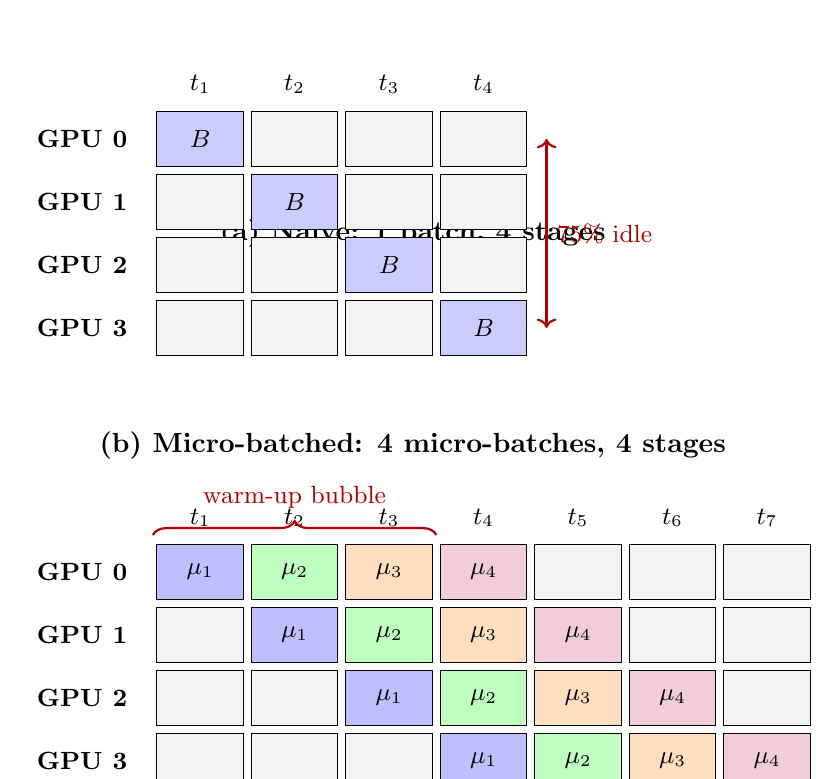
\begin{tikzpicture}[
    cell/.style={minimum width=1.1cm, minimum height=0.7cm, align=center, font=\small},
    active/.style={cell, draw, fill=blue!20},
    idle/.style={cell, draw, fill=gray!10, text=gray!50},
    label/.style={font=\small\bfseries, anchor=east},
    time/.style={font=\small, anchor=south},
]
% Title: Naive (no micro-batching)
\node[font=\bfseries] at (3.3, 1.2) {(a) Na\"ive: 1 batch, 4 stages};

% Stage labels
\node[label] at (-0.2, 0) {GPU 3};
\node[label] at (-0.2, 0.8) {GPU 2};
\node[label] at (-0.2, 1.6) {GPU 1};
\node[label] at (-0.2, 2.4) {GPU 0};

% Time labels (top, manually placed above row for GPU 0)
\foreach \t in {1,2,3,4} {
    \node[time] at ({(\t-1)*1.2+0.6}, 2.85) {$t_{\t}$};
}

% GPU 0: active at t1
\node[active] at (0.6, 2.4) {$B$};
\node[idle]   at (1.8, 2.4) {};
\node[idle]   at (3.0, 2.4) {};
\node[idle]   at (4.2, 2.4) {};
% GPU 1: active at t2
\node[idle]   at (0.6, 1.6) {};
\node[active] at (1.8, 1.6) {$B$};
\node[idle]   at (3.0, 1.6) {};
\node[idle]   at (4.2, 1.6) {};
% GPU 2: active at t3
\node[idle]   at (0.6, 0.8) {};
\node[idle]   at (1.8, 0.8) {};
\node[active] at (3.0, 0.8) {$B$};
\node[idle]   at (4.2, 0.8) {};
% GPU 3: active at t4
\node[idle]   at (0.6, 0) {};
\node[idle]   at (1.8, 0) {};
\node[idle]   at (3.0, 0) {};
\node[active] at (4.2, 0) {$B$};

% Bubble annotation
\draw[<->, thick, red!70!black] (5.0, 0) -- (5.0, 2.4) node[midway, right, font=\small, red!70!black] {75\% idle};

% Title: Micro-batched
\node[font=\bfseries] at (3.3, -1.5) {(b) Micro-batched: 4 micro-batches, 4 stages};

% Offset for second diagram
\begin{scope}[yshift=-5.5cm]
\node[label] at (-0.2, 0) {GPU 3};
\node[label] at (-0.2, 0.8) {GPU 2};
\node[label] at (-0.2, 1.6) {GPU 1};
\node[label] at (-0.2, 2.4) {GPU 0};

\foreach \t in {1,...,7} {
    \node[time] at ({(\t-1)*1.2+0.6}, 2.85) {$t_{\t}$};
}

% Color scheme for micro-batches
% m1=blue, m2=green, m3=orange, m4=purple
\tikzset{
    m1/.style={cell, draw, fill=blue!25},
    m2/.style={cell, draw, fill=green!25},
    m3/.style={cell, draw, fill=orange!25},
    m4/.style={cell, draw, fill=purple!20},
}

% GPU 0
\node[m1] at (0.6, 2.4) {$\mu_1$};
\node[m2] at (1.8, 2.4) {$\mu_2$};
\node[m3] at (3.0, 2.4) {$\mu_3$};
\node[m4] at (4.2, 2.4) {$\mu_4$};
\node[idle] at (5.4, 2.4) {};
\node[idle] at (6.6, 2.4) {};
\node[idle] at (7.8, 2.4) {};

% GPU 1
\node[idle] at (0.6, 1.6) {};
\node[m1] at (1.8, 1.6) {$\mu_1$};
\node[m2] at (3.0, 1.6) {$\mu_2$};
\node[m3] at (4.2, 1.6) {$\mu_3$};
\node[m4] at (5.4, 1.6) {$\mu_4$};
\node[idle] at (6.6, 1.6) {};
\node[idle] at (7.8, 1.6) {};

% GPU 2
\node[idle] at (0.6, 0.8) {};
\node[idle] at (1.8, 0.8) {};
\node[m1] at (3.0, 0.8) {$\mu_1$};
\node[m2] at (4.2, 0.8) {$\mu_2$};
\node[m3] at (5.4, 0.8) {$\mu_3$};
\node[m4] at (6.6, 0.8) {$\mu_4$};
\node[idle] at (7.8, 0.8) {};

% GPU 3
\node[idle] at (0.6, 0) {};
\node[idle] at (1.8, 0) {};
\node[idle] at (3.0, 0) {};
\node[m1] at (4.2, 0) {$\mu_1$};
\node[m2] at (5.4, 0) {$\mu_2$};
\node[m3] at (6.6, 0) {$\mu_3$};
\node[m4] at (7.8, 0) {$\mu_4$};

% Bubble annotation
\draw[decorate, decoration={brace, amplitude=5pt, raise=2pt}, thick, red!70!black]
    (0.0, 2.8) -- (3.6, 2.8) node[midway, above=8pt, font=\small, red!70!black] {warm-up bubble};
\end{scope}
\end{tikzpicture}
\caption{Pipeline bubble with and without micro-batching. (a)~Na\"ive pipeline parallelism with 4 stages: only one GPU is active per time step, wasting 75\% of GPU time. (b)~Micro-batched pipeline with 4 micro-batches ($\mu_1$--$\mu_4$): after the warm-up phase, all GPUs are active simultaneously. Gray cells are idle (bubble); colored cells are active. The bubble fraction drops from $3/4$ to $3/7 \approx 43\%$ with 4 micro-batches, and further decreases as $M$ grows.}
\label{fig:pipeline-bubble}
\end{figure}

\begin{insightbox}
Pipeline parallelism is complementary to tensor parallelism. A common configuration for very large models is TP within a node (using fast NVLink) and PP across nodes (using slower network interconnects). This exploits the communication characteristics of each strategy: TP requires frequent, fine-grained AllReduce operations ($2L$ per forward pass, needing high bandwidth), while PP requires infrequent, coarse-grained point-to-point transfers (one hidden-state tensor per micro-batch per stage boundary). For a hidden dimension of $d = 8192$ in FP16, a single point-to-point transfer is just $8192 \times 2 = 16$\,KB per token---easily handled even over InfiniBand.
\end{insightbox}

\subsection{PP for Inference vs.\ Training}

Pipeline parallelism was originally developed for training, where both the forward and backward passes create complex scheduling challenges (PipeDream, 1F1B schedules). For inference, the situation is simpler: there is only a forward pass, and the primary concern is latency rather than throughput. In inference, PP increases latency by the communication delay at each stage boundary, but it enables serving models that would not fit on a single node. For a LLaMA-405B model requiring 810\,GB of FP16 memory, a configuration of TP=8 within each node and PP=2 across two 8-GPU nodes distributes 810\,GB across 16 GPUs, requiring roughly 51\,GB per GPU---comfortably within the 80\,GB of an A100.

\begin{notebox}
The latency impact of pipeline parallelism during decode is multiplicative with the number of stages. Each decode step must traverse all pipeline stages sequentially. With 4 stages, a decode step that takes 10\,ms on a single GPU takes at least 10\,ms (the computation is the same, just distributed) plus communication overhead. However, the decode computation time itself decreases because each stage holds fewer layers and thus reads fewer weight bytes from HBM. The net effect depends on the relative costs of computation and communication.
\end{notebox}

\begin{whynotbox}{Why not pipeline the decode phase across requests?}
Micro-batching fills the pipeline by feeding multiple micro-batches in quick succession. During prefill, this works naturally: each micro-batch contains a chunk of tokens that can be processed independently. But during decode, each step generates just one token per request and depends on the previous step's output. Could we pipeline decode by staggering \emph{different requests} across pipeline stages?

\textbf{The dependency problem.} In principle, yes: while GPU~1 processes request~A's layers 21--40, GPU~0 could process request~B's layers 1--20. But the benefit is limited because each decode step is extremely fast (the computation per stage is tiny), so the pipeline communication latency at each stage boundary becomes a significant fraction of the stage compute time. With 4 stages and sub-millisecond compute per stage, even microsecond-scale NVLink transfers add meaningful overhead.

\textbf{In practice.} Continuous batching (Section~\ref{sec:distributed:batching}) is the preferred way to keep GPUs busy during decode: instead of pipelining across stages, it batches many requests together so that each stage processes a large batch of tokens simultaneously. This converts the problem from pipeline fill to batch fill, which is far easier to manage.
\end{whynotbox}

Pipeline parallelism and tensor parallelism address how to distribute the model's layers and weight matrices across GPUs. The next challenge is a different kind of efficiency: how to keep those GPUs busy across \emph{time}, by managing the flow of requests into and out of the system.

\section{Continuous Batching}
\label{sec:distributed:batching}

\marginnote{\emph{Continuous batching:} allowing requests to enter and exit the processing batch at any iteration, rather than waiting for the entire batch to complete.}%
Traditional (static) batching groups multiple requests together and processes them as a unit. All requests in a batch are padded to the same sequence length, and the batch is processed through the model as a single matrix operation. The batch is released only when \emph{every} request has finished generating. The problem is twofold:

\begin{enumerate}
\item \textbf{Head-of-line blocking.} If one request generates 10 tokens and another generates 1{,}000, the 10-token request's output is held until the 1{,}000-token request finishes---a 100$\times$ latency penalty.
\item \textbf{Wasted compute.} After a short request finishes, its slot in the batch continues to consume GPU compute (the model processes padding tokens) until the entire batch completes.
\end{enumerate}

\subsection{Iteration-Level Scheduling}

Continuous batching, introduced by the Orca system (Yu et al., 2022), solves both problems by operating at the granularity of individual decode iterations rather than full requests. At each decode step:

\begin{enumerate}
\item \textbf{Evict completed requests.} Any request that emitted a stop token is removed from the batch, and its KV cache blocks are freed.
\item \textbf{Insert new requests.} Any waiting request is added to the batch. Its prompt is prefilled (or, in some implementations, prefill is deferred to a separate phase).
\item \textbf{Decode.} All active requests in the batch advance by one token.
\end{enumerate}

This dramatically improves both throughput and latency. Throughput increases because GPU cycles are never wasted on completed requests---the batch remains full as long as there are waiting requests. Latency improves because short requests are returned immediately upon completion, not blocked by long ones.

\begin{notebox}
Continuous batching interacts with PagedAttention (Chapter~\ref{ch:kvcache}) in a critical way. Because PagedAttention allocates KV cache blocks dynamically from a shared pool, the scheduler can add new requests to the batch as long as free blocks are available---without pre-allocating a fixed maximum cache size per request. This synergy between dynamic batching and dynamic memory management is what makes high-throughput serving practical. Without PagedAttention, the scheduler would need to reserve worst-case cache memory for each request slot, dramatically limiting the batch size.
\end{notebox}

\subsection{Quantifying the Throughput Gain}

Consider a static batch of $B = 32$ requests, where generation lengths are uniformly distributed between 50 and 500 tokens. The expected longest generation is approximately 500 tokens (the maximum). Under static batching, all 32 requests run for 500 iterations, consuming $32 \times 500 = 16{,}000$ GPU-iterations. The useful work is $32 \times 275 = 8{,}800$ GPU-iterations (using the expected generation length of 275). The utilization is $8{,}800 / 16{,}000 = 55\%$.

Under continuous batching, each completed request's slot is immediately refilled. If the arrival rate is sufficient to keep the batch full, utilization approaches 100\%. Moreover, the total number of requests served in the time it takes to generate 500 tokens is not 32---it is approximately $32 \times 500 / 275 \approx 58$ requests, an 81\% throughput improvement over static batching.

\subsection{Prefill-Decode Interference}

\marginnote{Prefill-decode interference is a primary motivation for disaggregated serving (Section~\ref{sec:distributed:disaggregated}).}%
There is a subtlety: when a new request enters the continuous batch, its prompt must be prefilled---a compute-intensive operation that processes all input tokens in parallel. This prefill computation shares the GPU with ongoing decode iterations for other requests. Because prefill has much higher arithmetic intensity than decode, it can delay the decode iterations, causing latency spikes for in-flight requests. This \emph{prefill-decode interference} is one of the key challenges of continuous batching, and a major motivation for disaggregated serving (Section~\ref{sec:distributed:disaggregated}).


\section{Speculative Decoding}
\label{sec:distributed:speculative}

\marginnote{\emph{Speculative decoding:} using a small ``draft'' model to propose multiple tokens, then verifying them in parallel with the large model.}%
Standard autoregressive decoding generates one token per forward pass, which is inherently sequential. Each decode step reads the full model weights from HBM, but performs only enough computation for a single token. Speculative decoding (Leviathan et al., 2023; Chen et al., 2023) breaks this bottleneck by exploiting the gap between the model's arithmetic capacity and its memory bandwidth utilization.

\subsection{The Algorithm}

The procedure has three steps:

\begin{enumerate}
\item \textbf{Draft.} A small, fast \emph{draft model} $M_q$ (e.g., a 1B-parameter variant of the target model) generates $k$ candidate tokens $\hat{t}_1, \hat{t}_2, \ldots, \hat{t}_k$ autoregressively. Because the draft model is small, each step is fast.
\item \textbf{Verify.} The large \emph{target model} $M_p$ processes all $k$ candidates in a single forward pass (as if they were a prompt of length $k$). This produces the target model's probability distributions $p(\cdot \mid t_1, \ldots, t_{i-1})$ for each position $i = 1, \ldots, k$.
\item \textbf{Accept/reject.} For each position $i$ from left to right: the token is accepted with probability $\min(1,\; p(t_i)/q(t_i))$---which means acceptance is certain whenever $q(t_i) \leq p(t_i)$. If rejected, a corrected token is sampled from an adjusted distribution $\text{norm}(\max(0, p - q))$. All subsequent draft tokens are discarded.
\end{enumerate}

\begin{insightbox}
The verification step is mathematically exact: the accept/reject scheme guarantees that the output distribution is \emph{identical} to what the target model would produce alone. Speculative decoding is not an approximation---it is a lossless acceleration technique. The proof relies on the fact that the adjusted sampling distribution at each rejected position exactly compensates for the bias introduced by the draft model.
\end{insightbox}

\subsection{Speedup Analysis}

Let $\alpha$ denote the average acceptance rate---the probability that the target model accepts a draft token. If the draft model generates $k$ candidates and the target model verifies them in one pass, the expected number of tokens generated per verification step is:

\begin{equation}
\label{eq:spec-tokens}
\mathbb{E}[\text{tokens per step}] = \frac{1 - \alpha^{k+1}}{1 - \alpha}
\end{equation}

\noindent For $\alpha = 0.8$ and $k = 5$:

\begin{equation}
\mathbb{E}[\text{tokens per step}] = \frac{1 - 0.8^6}{1 - 0.8} = \frac{1 - 0.262}{0.2} = 3.69 \;\text{tokens}
\end{equation}

If the verification step (one forward pass of the target model on $k$ tokens) takes roughly the same time as $k$ standard decode steps, the speedup is modest. But here is the key insight: during decode, the target model is \emph{memory-bound}. Processing $k$ tokens costs nearly the same wall time as processing 1 token, because the bottleneck is reading the weights from HBM, not the arithmetic. The model weights are read once regardless of whether we compute attention for 1 position or $k$ positions. The speedup is therefore approximately:

\begin{equation}
\label{eq:spec-speedup}
\text{Speedup} \approx \frac{1 - \alpha^{k+1}}{(1 - \alpha)(1 + c)}
\end{equation}

\noindent where $c$ is the relative cost of running the draft model (typically $c \approx 0.05$--$0.1$ for a well-chosen small draft model). With $\alpha = 0.8$, $k = 5$, and $c = 0.07$:

\begin{equation}
\text{Speedup} \approx \frac{3.69}{1.07} \approx 3.4\times
\end{equation}

In practice, speedups of 2--3$\times$ are common for well-matched draft-target pairs. The acceptance rate $\alpha$ depends heavily on the quality of the draft model and the difficulty of the text being generated: predictable code completions achieve higher acceptance rates than creative writing.

\begin{notebox}
\textbf{Draft model selection.} The draft model must share the same vocabulary and tokenizer as the target model. Common choices include: (a) a smaller model from the same family (e.g., LLaMA-1B drafting for LLaMA-70B), (b) a model obtained by pruning or distilling the target, or (c) a simple $n$-gram model or retrieval-based predictor. The trade-off is clear: a better draft model increases $\alpha$ but also increases $c$. Medusa (Cai et al., 2024) takes a different approach, adding lightweight ``heads'' to the target model itself that predict multiple future tokens in parallel, avoiding the need for a separate draft model entirely.
\end{notebox}

\begin{whynotbox}{Why not use a draft model from a different model family?}
The draft model must share the target model's tokenizer and vocabulary. If the draft model uses a different tokenizer, the token IDs in the draft sequence do not correspond to the same tokens in the target model, and the accept/reject scheme---which compares per-token probabilities $p(t_i)$ and $q(t_i)$---becomes meaningless.

\textbf{Beyond vocabulary.} Even with a shared vocabulary, the draft and target models should have similar ``styles'' of prediction. A draft model trained on code may produce poor acceptance rates when the target model generates prose, because the draft's high-confidence predictions diverge from the target's distribution. This is why same-family models (e.g., LLaMA-1B drafting for LLaMA-70B) typically achieve the highest acceptance rates: they were trained on similar data with similar objectives, so their probability distributions are well-aligned.

\textbf{The Medusa alternative.} If finding a compatible draft model is difficult, Medusa sidesteps the issue entirely by attaching lightweight prediction heads directly to the target model's hidden states. These heads are trained to predict future tokens from the same representation, guaranteeing distribution alignment by construction.
\end{whynotbox}

Speculative decoding accelerates the generation loop by producing multiple tokens per forward pass. But it does not address the fundamental tension between the prefill and decode phases---they have different computational profiles and compete for GPU resources. The next section tackles this structural problem head-on.

\section{Disaggregated Serving}
\label{sec:distributed:disaggregated}

\marginnote{\emph{Disaggregated serving:} running prefill and decode on separate GPU pools, independently scaled.}%
The prefill phase (processing the input prompt) and the decode phase (generating tokens one at a time) have fundamentally different computational profiles that are at odds with each other.

\subsection{The Compute Profile Mismatch}

During \textbf{prefill}, the model processes all $n$ input tokens in parallel. The computation is a sequence of large matrix-matrix multiplications ($\mathbf{X} \mathbf{W}$ where $\mathbf{X} \in \mathbb{R}^{n \times d}$), achieving high arithmetic intensity:

\begin{equation}
\label{eq:prefill-intensity}
\text{Arithmetic intensity (prefill)} = \frac{2 \cdot n \cdot P}{2P} = n \;\text{FLOP/byte}
\end{equation}

\noindent For a prompt of $n = 2048$ tokens, the arithmetic intensity is 2048 FLOP/byte---well above the A100's compute-to-bandwidth ratio of 156 FLOP/byte. Prefill is \emph{compute-bound}: the GPU's arithmetic units are the bottleneck, and HBM bandwidth is fully utilized.

During \textbf{decode}, as we computed in Section~\ref{sec:distributed:bottleneck}, the arithmetic intensity is just 1 FLOP/byte. Decode is \emph{memory-bandwidth-bound}: the arithmetic units are almost entirely idle.

\begin{table}[h]
\centering
\begin{tabular}{lcc}
\toprule
\textbf{Property} & \textbf{Prefill} & \textbf{Decode} \\
\midrule
Tokens processed & $n$ (prompt length) & 1 \\
Arithmetic intensity & $n$ FLOP/byte & 1 FLOP/byte \\
Bottleneck & Compute (FLOPS) & Memory bandwidth \\
Batch dimension & Sequence length & Batch size \\
Latency metric & Time-to-first-token & Inter-token latency \\
\bottomrule
\end{tabular}
\caption{The fundamental asymmetry between prefill and decode. Prefill is compute-bound because it processes many tokens at once. Decode is memory-bandwidth-bound because it processes one token at a time.}
\label{tab:prefill-decode}
\end{table}

\subsection{Why Co-location Hurts}

When prefill and decode share the same GPU (as in most serving systems), they interfere destructively:

\begin{enumerate}
\item \textbf{Decode latency spikes.} When a new request's prefill begins, it consumes the GPU's compute resources for tens of milliseconds (for a long prompt). During this time, all in-flight decode requests are stalled. Users see a sudden pause in token generation.
\item \textbf{Resource mismatch.} The optimal GPU for prefill (high FLOPS) may differ from the optimal GPU for decode (high HBM bandwidth). Co-location forces a compromise.
\item \textbf{Scaling inflexibility.} A workload dominated by long prompts needs more prefill capacity. A workload dominated by long generations needs more decode capacity. With co-located serving, you must scale both together.
\end{enumerate}

\subsection{The Disaggregated Architecture}

Disaggregated serving, as implemented in Dynamo, separates prefill and decode onto different GPU pools. The architecture operates in three phases:

\begin{enumerate}
\item \textbf{Prefill.} A prefill worker processes the input prompt, computing the full forward pass and generating the initial KV cache.
\item \textbf{KV cache transfer.} The computed KV cache is transferred from the prefill worker to a decode worker over the network. For a 70B model with GQA (8 KV heads), $d_k = 128$, and a prompt of 2048 tokens, the KV cache size is:
\begin{equation}
\label{eq:kv-transfer}
2 \times L \times n_{\text{kv}} \times d_k \times n \times 2 = 2 \times 80 \times 8 \times 128 \times 2048 \times 2 \approx 671\;\text{MB}
\end{equation}
This must be transferred over the network, typically via RDMA (Remote Direct Memory Access) for GPU-to-GPU transfers.
\item \textbf{Decode.} The decode worker receives the KV cache and generates tokens autoregressively, appending new KV entries at each step.
\end{enumerate}

\marginnote{Dynamo uses NVIDIA's NIXL library for high-performance GPU-to-GPU memory transfers, enabling RDMA-based KV cache transfer between prefill and decode workers without CPU involvement.}%
The KV cache transfer introduces latency---671\,MB at 25\,GB/s (100 Gbps InfiniBand) takes approximately 27\,ms. This transfer cost must be weighed against the interference cost of co-location. For long prompts (large prefill compute) and many concurrent decode requests (where interference is severe), disaggregation provides a net benefit.

\begin{insightbox}
Disaggregated serving is the key architectural insight that distinguishes Dynamo from simpler inference systems. By separating the compute-bound prefill from the memory-bound decode, each phase runs on hardware optimized for its computational profile. The router (Chapter~\ref{ch:kvrouter}) must now make a two-stage decision: first, which prefill worker should process the prompt (optimizing for cache reuse and compute availability), and second, which decode worker should receive the KV cache (optimizing for memory bandwidth availability and load balance). This two-stage routing is fundamentally more complex than single-pool routing, but it enables independent scaling of each phase---a capability that is essential for cost-effective serving of diverse workloads.
\end{insightbox}

\subsection{Independent Scaling}

The power of disaggregation becomes clear when workload characteristics vary. Consider two scenarios:

\textbf{Scenario A: Summarization workload.} Users submit long documents (8K--32K tokens) and request short summaries (100--200 tokens). Prefill dominates. The system needs many prefill workers but few decode workers.

\textbf{Scenario B: Code generation.} Users submit short prompts (100--500 tokens) and request long completions (1K--4K tokens). Decode dominates. The system needs few prefill workers but many decode workers.

With co-located serving, both scenarios require the same number of GPUs (scaled to the dominant phase), wasting resources on the non-dominant phase. With disaggregated serving, the prefill and decode pools scale independently, potentially halving GPU costs for skewed workloads. Dynamo's planner component monitors active prefill tokens and active decode blocks on each worker, dynamically scaling each pool based on current demand.


\section{Putting It All Together}
\label{sec:distributed:together}

These five techniques are not mutually exclusive---they compose. A production deployment of a 405B-parameter model might use:

\begin{itemize}
\item \textbf{Tensor parallelism (TP=8)} within each 8-GPU node, splitting every layer's weight matrices across all 8 GPUs connected by NVLink.
\item \textbf{Pipeline parallelism (PP=4)} across 4 nodes, assigning roughly 32 of the model's 126 layers to each node.
\item \textbf{Continuous batching} to keep the GPU pipeline full by dynamically inserting and evicting requests at each decode iteration.
\item \textbf{Speculative decoding} with a 1B draft model to generate 3--4 tokens per target-model forward pass.
\item \textbf{Disaggregated serving} to separate prefill onto a dedicated pool of high-FLOPS GPUs and decode onto a pool optimized for HBM bandwidth.
\end{itemize}

The total GPU count in this configuration is $8 \times 4 = 32$ GPUs per model replica, with additional GPUs in the disaggregated decode pool. The system collectively provides $32 \times 3.35 = 107$\,TB/s of aggregate HBM bandwidth (H100), enabling decode throughput orders of magnitude beyond what a single GPU can achieve.


\section{Summary}

\begin{itemize}
  \item The \textbf{single-GPU bottleneck} is both memory capacity (a 70B FP16 model needs 140\,GB; an A100 has 80\,GB) and memory bandwidth (decode arithmetic intensity is 1 FLOP/byte, 156$\times$ below the A100's compute-to-bandwidth ratio).
  \item \textbf{Tensor parallelism} splits weight matrices across GPUs for latency reduction: columns of $\mathbf{W}_1$, rows of $\mathbf{W}_2$ in the FFN; attention heads across GPUs. Requires $2L$ AllReduce operations per forward pass, demanding high-bandwidth NVLink interconnects.
  \item \textbf{Pipeline parallelism} assigns layers to different GPUs, with bubble fraction $(N-1)/(N+M-1)$ when using $M$ micro-batches. Requires only point-to-point communication at stage boundaries, making it suitable for cross-node deployment.
  \item \textbf{Continuous batching} allows requests to enter and exit the batch at each iteration, eliminating the head-of-line blocking of static batching. Interacts synergistically with PagedAttention for dynamic KV cache allocation.
  \item \textbf{Speculative decoding} uses a draft model to propose $k$ tokens verified in one target-model pass, achieving 2--3$\times$ speedup without approximation. Exploits the memory-bound nature of decode: verifying $k$ tokens costs nearly the same wall time as generating 1.
  \item \textbf{Disaggregated serving} separates compute-bound prefill from memory-bound decode, enabling independent scaling and eliminating cross-phase interference. Requires KV cache transfer over the network.
\end{itemize}

\bigskip
\begin{center}\rule{0.5\linewidth}{0.4pt}\end{center}
\bigskip

We now have the conceptual tools to understand every major component of Dynamo. The next chapter traces a request end-to-end through the system, showing how these distributed inference techniques are composed into a working architecture.

\bigskip
\noindent\textbf{Check Your Understanding}

\medskip
\noindent\emph{These questions are answerable from this chapter alone.}

\begin{enumerate}
  \item Why is LLM decode memory-bound rather than compute-bound? What is the arithmetic intensity of a single-token decode step?

  \textbf{Answer:} A single-token decode step performs approximately $2P$ FLOPs (one multiply-add per parameter) but must read all $2P$ bytes of model weights (in FP16) from HBM. The arithmetic intensity is therefore $2P / 2P = 1$ FLOP/byte. The A100's compute-to-bandwidth ratio is 156 FLOP/byte, meaning the GPU is 156$\times$ more capable of computation than the memory system can feed it. The GPU's arithmetic units sit mostly idle, waiting for weight data.

  \item Tensor parallelism and pipeline parallelism both distribute a model across GPUs, but they have different communication patterns. Which requires higher interconnect bandwidth, and why?

  \textbf{Answer:} Tensor parallelism requires higher interconnect bandwidth. It performs $2L$ AllReduce operations per forward pass (two per transformer layer: one for attention, one for FFN), each synchronizing all participating GPUs. Pipeline parallelism requires only point-to-point transfers of hidden-state tensors at stage boundaries---one transfer per micro-batch per boundary, with each transfer being just $d \times \text{sizeof(FP16)}$ bytes per token. This is why TP is used within a node (NVLink, 900\,GB/s) and PP is used across nodes (InfiniBand, 25--100\,GB/s).

  \item In the Megatron-LM FFN partitioning scheme, why is $\mathbf{W}_1$ split by columns and $\mathbf{W}_2$ split by rows, rather than the reverse?

  \textbf{Answer:} Splitting $\mathbf{W}_1$ by columns means each GPU computes a complete slice of the hidden representation (a subset of the $d_{\text{ff}}$ dimensions). The nonlinear activation function $\sigma$ can then be applied locally on each GPU without any communication. If $\mathbf{W}_1$ were split by rows instead, each GPU would produce a partial sum of the full hidden vector, requiring an AllReduce \emph{before} applying the activation function---doubling the total communication from 2 AllReduce operations per layer to 4.

  \item Explain why continuous batching improves both throughput and latency compared to static batching.

  \textbf{Answer:} Throughput improves because completed requests are immediately evicted and their slots refilled with new requests, keeping the batch full at all times. Under static batching, completed requests waste GPU cycles until the longest request finishes. Latency improves because short requests are returned as soon as they finish generating, rather than waiting for the longest request in the batch. A 10-token request in a static batch with a 1{,}000-token request waits 1{,}000 iterations; with continuous batching, it waits only 10.

  \item Speculative decoding is described as producing output \emph{identical} to standard decoding. How is this possible if the draft model makes incorrect predictions?

  \textbf{Answer:} The accept/reject scheme ensures mathematical equivalence. When the draft model's prediction is rejected at position $i$, the system does not simply use the target model's top prediction. Instead, it samples from an adjusted distribution $\text{norm}(\max(0, p - q))$ that exactly compensates for the bias introduced by accepting some of the draft model's tokens. This ensures that the overall probability of generating any particular token sequence is identical to sampling directly from the target model. The draft model affects only the \emph{speed}, never the \emph{distribution} of the output.

  \item For a 70B model with 80 layers, 8 KV heads, $d_k = 128$, and a 4096-token prompt, calculate the KV cache size that must be transferred during disaggregated serving.

  \textbf{Answer:} The KV cache stores both keys and values (factor of 2), for each layer (80), for each KV head (8), with dimension $d_k = 128$, for each token (4096), in FP16 (2 bytes): $2 \times 80 \times 8 \times 128 \times 4096 \times 2 = 1{,}342{,}177{,}280$ bytes $\approx 1.34$\,GB. At 25\,GB/s (100 Gbps InfiniBand with RDMA), this transfer takes approximately 54\,ms.

  \item Disaggregated serving introduces a new cost: KV cache transfer between prefill and decode workers. Under what conditions is this trade-off favorable?

  \textbf{Answer:} The trade-off is favorable when the interference cost of co-located prefill and decode exceeds the transfer cost. This occurs when: (a) prompts are long, making prefill compute-intensive and the resulting decode latency spikes severe; (b) many decode requests are in-flight simultaneously, meaning a single prefill delays many users; (c) the network supports high-bandwidth GPU-to-GPU transfers (RDMA/NIXL), keeping transfer latency low. For short prompts with few concurrent users, the transfer overhead may exceed the interference savings, making co-location preferable.

  \item A deployment uses TP=8 within each node and PP=2 across nodes. The model has 80 layers and $d = 8192$. How many AllReduce operations occur per forward pass, and how many point-to-point transfers occur per micro-batch?

  \textbf{Answer:} Each of the 80 layers requires 2 AllReduce operations (one for attention output, one for FFN output), giving $2 \times 80 = 160$ AllReduce operations per forward pass. Each AllReduce involves 8 GPUs within a node via NVLink. For pipeline parallelism with 2 stages, there is 1 stage boundary, requiring 1 point-to-point transfer of the hidden-state tensor per micro-batch (from node 0 to node 1). This transfer is $8192 \times 2 = 16$\,KB per token in the micro-batch, sent over the inter-node network.
\end{enumerate}

\chapter{Dynamo Architecture End-to-End}
\label{ch:architecture}

The previous chapters introduced the building blocks: transformer attention, KV caching, and distributed inference techniques. This chapter assembles them into the concrete system that is NVIDIA Dynamo. We trace a single request from the moment it arrives as an HTTP payload to the moment the last token streams back to the client, identifying every component it touches along the way. By the end, you will have a complete map of Dynamo's architecture---what each component does, why it exists, and how it communicates with its neighbors.

%% ============================================================
\section{A Request's Journey}
\label{sec:architecture:journey}
%% ============================================================

\marginnote{\emph{SSE (Server-Sent Events):} a standard for streaming data from server to client over HTTP.}%
Consider a user sending a chat completion request to a Dynamo cluster serving a large language model. The request begins its life as an HTTP POST carrying a JSON payload conforming to the OpenAI chat completions API---a format Dynamo deliberately supports for compatibility with the broader ecosystem. Let us trace every component the request touches.

\subsection{Stage 1: HTTP Ingress}

The request arrives at the \textbf{frontend server}, an async Rust HTTP service built on \texttt{axum} (a Tokio-based web framework). The frontend is implemented in the \texttt{dynamo-llm} crate's \texttt{http::\allowbreak service::\allowbreak service\_v2} module, which exposes OpenAI-compatible endpoints (\texttt{/v1/chat/\allowbreak completions}, \texttt{/v1/\allowbreak completions}, \texttt{/v1/\allowbreak embeddings}), plus Anthropic-format endpoints for messages. The frontend validates the incoming JSON, checks whether the requested model is registered (via a \texttt{ModelManager} that watches the service discovery plane), and determines whether the client wants a streaming or non-streaming response.

\begin{notebox}
Regardless of whether the client requests \texttt{stream=true} or \texttt{stream=false}, Dynamo internally propagates all requests as streaming. This simplifies the downstream pipeline to a single pattern: every request returns a stream of token fragments. For non-streaming client requests, the frontend aggregates the entire stream into a single JSON response before sending it back. This design decision eliminates an entire class of code paths and their associated bugs.
\end{notebox}

\subsection{Stage 2: Preprocessing}

The validated request is handed to the \textbf{preprocessor} (in \texttt{dynamo-llm}'s \texttt{preprocessor} module). The preprocessor performs two critical transformations:

\begin{enumerate}
  \item \textbf{Chat template application.} The user's message array (\texttt{[{"role":"user","content":"Hello"}]}) must be converted into the specific prompt format that the model was trained on. Dynamo uses \texttt{minijinja}, a Rust implementation of the Jinja2 template engine, to apply model-specific chat templates. Different models require wildly different formats---Llama uses \texttt{<|begin\_of\_text|>} markers, ChatGLM uses \texttt{[gMASK]<sop>}, and Mistral uses \texttt{[INST]} tags. The template is loaded from the model's configuration at startup.

  \item \textbf{Tokenization.} The formatted prompt string is tokenized into a sequence of integer token IDs using the \texttt{dynamo-llm} tokenizer module, which wraps the Hugging Face \texttt{tokenizers} library (itself a Rust crate with Python bindings). For models that use OpenAI's encoding, Dynamo falls back to \texttt{tiktoken-rs}. The result is a \texttt{Vec<u32>} of token IDs ready for the model.
\end{enumerate}

\marginnote{The preprocessor also handles media: images, audio, and video are fetched, decoded, and converted to tensor representations in this stage.}%

With the prompt tokenized into a sequence of integer IDs, the system must now decide \emph{where} to send it. This is not a simple load-balancing decision---it depends on the state of every GPU's memory.

\subsection{Stage 3: Routing}

\marginnote{\emph{Stateful routing:} routing decisions that depend on the current state of the cluster (e.g., cached data), as opposed to stateless policies like round-robin.}%
The token sequence now reaches the \textbf{router}, the most architecturally distinctive component in Dynamo. The router must answer the question: \emph{which GPU worker should process this request?}

In conventional load balancers, routing is stateless---round-robin or least-connections. Dynamo's router is \emph{stateful}: it knows what KV cache blocks each worker currently holds in GPU memory. This knowledge comes from the \textbf{KV indexer}, a concurrent radix tree (Chapter~\ref{ch:kvrouter}) that maps token block hashes to worker IDs.

The routing process works as follows:

\begin{enumerate}
  \item The router hashes the token sequence into fixed-size blocks using the \texttt{dynamo-tokens} crate's block hasher (Chapter~\ref{ch:tokens}). Each block of $B$ consecutive tokens is hashed with xxHash to produce a \texttt{LocalBlockHash}.

  \item The router queries the radix tree for overlap scores: for each candidate worker, how many of the request's token blocks are already cached on that worker?

  \item A \textbf{worker selector} (in \texttt{dynamo-kv-router}'s \texttt{scheduling::selector} module) combines the overlap score with the worker's current load (queue depth, active sequences, available KV cache capacity) to produce a composite cost. The worker with the lowest cost is selected.

  \item If KV-aware routing is not enabled, the router falls back to round-robin or random selection via the \texttt{RouterMode} enum (\texttt{RoundRobin}, \texttt{Random}, \texttt{KV}, or \texttt{Direct}).
\end{enumerate}

The router is implemented as a \texttt{PushRouter} in \texttt{dynamo-runtime}'s pipeline framework. The KV-specific variant, \texttt{KvPushRouter} (in \texttt{dynamo-llm}'s \texttt{kv\_router::push\_router} module), wraps the generic \texttt{PushRouter} with KV-aware selection logic.

\begin{insightbox}
The router is where Dynamo's core innovation lives. Traditional inference serving systems treat GPU workers as interchangeable---any worker can handle any request. By tracking KV cache state across the cluster, Dynamo can route a request to the worker that already has the most relevant cached computation, turning a full prefill (potentially seconds) into a partial prefill (milliseconds). The cost is maintaining a distributed index of cache contents, which is exactly what the radix tree provides.
\end{insightbox}

\subsection{Stage 4: Request Dispatch}

\marginnote{The \texttt{TwoPartCodec} uses a 24-byte preamble: 8 bytes for header length, 8 bytes for body length, 8 bytes for an xxHash checksum. See Chapter~\ref{ch:codecs} for details.}%
Once the router selects a worker, the request is serialized and dispatched. Dynamo supports three transport modes for the \emph{request plane}, configured via the \texttt{TransportType} enum:

\begin{itemize}
  \item \texttt{Nats}: Messages are published to NATS subjects. The worker subscribes to its designated subject and dequeues requests. This mode uses NATS as a work queue with load balancing across subscribers in the same queue group.
  \item \texttt{Http}: Requests are sent over HTTP/2 to the worker's advertised address.
  \item \texttt{Tcp}: Requests are sent over persistent TCP connections using the custom \texttt{TwoPartCodec} binary protocol, which avoids the overhead of HTTP framing.
\end{itemize}

In the TCP path, the \texttt{TcpRequestMessage} carries the endpoint path (for routing within the worker), optional trace headers (for distributed tracing via OpenTelemetry), and the serialized payload.

\begin{whynotbox}{Why not use gRPC instead of a custom TCP codec?}
gRPC is the standard choice for inter-service communication in distributed systems, and Dynamo does use gRPC for some ancillary services. But the hot path---router to worker, worker to frontend---uses a custom \texttt{TwoPartCodec} over raw TCP instead. Why?

\textbf{Framing overhead.} gRPC is built on HTTP/2, which adds frame headers, stream multiplexing metadata, HPACK-compressed headers, and WINDOW\_UPDATE flow control frames to every message. The \texttt{TwoPartCodec} uses a fixed 24-byte preamble (header length, body length, xxHash checksum) and nothing else. At thousands of messages per second per worker, those extra bytes and the CPU cycles to process them add up.

\textbf{Serialization coupling.} gRPC mandates Protocol Buffers for serialization. Dynamo's internal messages are already Rust structs serialized with \texttt{serde}---adding a Protobuf layer would mean double serialization (Rust $\to$ serde $\to$ bytes $\to$ Protobuf $\to$ bytes) or a rewrite of all internal types as \texttt{.proto} files. The custom codec serializes Rust types directly via \texttt{bincode} or MessagePack, with zero intermediate copies.

\textbf{Streaming model.} gRPC's streaming RPCs add per-message length-prefixed framing within the HTTP/2 stream. For token-by-token streaming where each message is tiny (a single token ID plus metadata), the framing overhead can exceed the payload size. The \texttt{TwoPartCodec} separates the header (routing metadata) from the body (payload) at the wire level, enabling the router to inspect headers without deserializing the body.

gRPC remains an excellent choice when interoperability with external clients matters more than raw throughput---which is why Dynamo exposes gRPC endpoints in \texttt{dynamo-llm} for external integrations alongside the internal TCP path.
\end{whynotbox}

\subsection{Stage 5: Inference}

The worker receives the request and feeds it to the \textbf{inference engine}. Dynamo does not implement its own GPU kernels for transformer inference; instead, it orchestrates existing engines:

\begin{itemize}
  \item \textbf{vLLM}: a Python-based engine with PagedAttention for efficient KV cache management.
  \item \textbf{SGLang}: a fast serving framework with RadixAttention.
  \item \textbf{TensorRT-LLM}: NVIDIA's optimized C++ inference engine with INT4/INT8 quantization.
\end{itemize}

Each engine is wrapped in a \texttt{PythonAsyncEngine} (via PyO3, discussed in Section~\ref{sec:architecture:pyo3}), which exposes the Python engine's async generator as a Rust \texttt{AsyncEngine} trait object. The engine produces tokens one at a time as an async stream.

\marginnote{In disaggregated mode, prefill workers and decode workers are separate GPU pools. The prefill worker computes the KV cache and transfers it to the decode worker via NIXL before token generation begins.}%

\marginnote{\emph{Disaggregated serving:} separating the prefill phase (compute-bound) from the decode phase (memory-bandwidth-bound) onto different GPU pools, each independently scaled.}%
In a \textbf{disaggregated configuration}, the request may touch two workers:
\begin{enumerate}
  \item A \textbf{prefill worker} processes the full prompt, computing the KV cache for all input tokens. This is compute-bound (proportional to sequence length squared for attention).
  \item The KV cache is transferred to a \textbf{decode worker} via NVIDIA's NIXL library, which performs direct GPU-to-GPU memory transfers without CPU involvement.
  \item The decode worker generates tokens autoregressively, one per iteration. This is memory-bandwidth-bound (each iteration reads the full model weights but produces only one token).
\end{enumerate}

The \texttt{PrefillRouter} (in \texttt{dynamo-llm}'s \texttt{kv\_router::prefill\_router} module) handles the prefill-to-decode handoff, using the \texttt{BlockManager} to coordinate NIXL transfers.

\subsection{Stage 6: Response Streaming}

Each generated token flows back through the pipeline in reverse. The worker wraps each token in an \texttt{Annotated<LLMEngineOutput>}---a protocol wrapper that carries both the token data and metadata (timing information, finish reason, usage statistics). The stream of annotated outputs travels back through the transport layer to the frontend, which converts each into a Server-Sent Event conforming to the OpenAI streaming format:

\begin{verbatim}
data: {"id":"chatcmpl-abc","choices":[{"delta":{"content":" world"}}]}
\end{verbatim}

When the model emits a stop token or reaches the maximum generation length, the stream closes with a \texttt{[DONE]} sentinel. The worker's \texttt{RequestGuard} (a drop guard in the \texttt{KvPushRouter}) fires, recording latency metrics, calling \texttt{free()} on the allocated KV cache blocks in the radix tree, and updating the worker's load statistics.

\begin{notebox}
The entire journey---from HTTP request to first token---is called \emph{time to first token} (TTFT). The time between subsequent tokens is the \emph{inter-token latency} (ITL). These two metrics dominate user-perceived quality: TTFT determines how long the user waits before seeing any output, while ITL determines the speed of the streaming response. Dynamo's architecture is optimized to minimize both---KV-aware routing reduces TTFT by maximizing cache hits, while disaggregated serving allows decode workers to specialize for low ITL.
\end{notebox}

% --- Request flow diagram ---
\begin{figure}[ht]
\centering
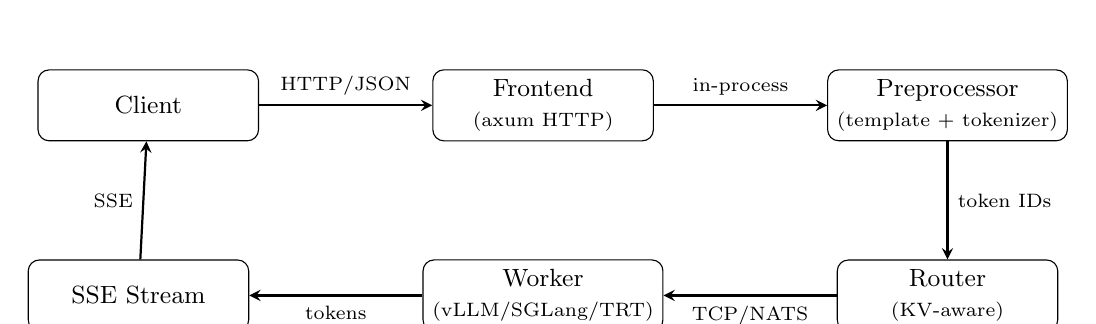
\begin{tikzpicture}[
    node distance=1.8cm and 2.2cm,
    box/.style={rectangle, draw, rounded corners, minimum width=2.8cm, minimum height=0.9cm, align=center, font=\small},
    arrow/.style={->, thick, >=stealth},
    label/.style={font=\scriptsize, midway, above},
    labelbelow/.style={font=\scriptsize, midway, below}
]
  % Nodes
  \node[box] (client) {Client};
  \node[box, right=of client] (frontend) {Frontend\\{\scriptsize(axum HTTP)}};
  \node[box, right=of frontend] (preproc) {Preprocessor\\{\scriptsize(template + tokenizer)}};
  \node[box, below=1.5cm of preproc] (router) {Router\\{\scriptsize(KV-aware)}};
  \node[box, left=of router] (worker) {Worker\\{\scriptsize(vLLM/SGLang/TRT)}};
  \node[box, left=of worker] (response) {SSE Stream};

  % Arrows
  \draw[arrow] (client) -- (frontend) node[label] {HTTP/JSON};
  \draw[arrow] (frontend) -- (preproc) node[label] {in-process};
  \draw[arrow] (preproc) -- (router) node[label, right] {token IDs};
  \draw[arrow] (router) -- (worker) node[labelbelow] {TCP/NATS};
  \draw[arrow] (worker) -- (response) node[labelbelow] {tokens};
  \draw[arrow] (response) -- (client) node[label, left] {SSE};
\end{tikzpicture}
\caption{The journey of a single inference request through Dynamo's pipeline. The hot path (router, codec, transport) is Rust; the inference engine is Python.}
\label{fig:request-journey}
\end{figure}

%% ============================================================
\section{Service Discovery}
\label{sec:architecture:discovery}
%% ============================================================

The request journey above assumed the router already knew which workers exist and where they are. But in a dynamic cluster---where workers start, crash, and scale independently---this knowledge cannot be hardcoded. How does the router find its workers? That is the job of service discovery.

\marginnote{\emph{etcd:} a distributed key-value store used for service registration and configuration. NATS JetStream provides an alternative KV store backend for simpler deployments.}%
Dynamo operates as a fleet of independently deployed services: frontend servers, routers, prefill workers, decode workers, and auxiliary services. Each must find and communicate with the others without hardcoded addresses. Dynamo solves this with a \textbf{pluggable discovery system} defined by the \texttt{Discovery} trait in \texttt{dynamo-runtime}'s \texttt{discovery} module.

\subsection{The Discovery Trait}

The \texttt{Discovery} trait (at \texttt{lib/runtime/src/discovery/mod.rs}) defines five operations:

\begin{enumerate}
  \item \texttt{instance\_id()} --- returns the unique identifier for this worker (typically an etcd lease ID or a generated hash).
  \item \texttt{register(spec)} --- publishes a \texttt{DiscoverySpec} (endpoint, model card, or event channel) to the discovery plane.
  \item \texttt{unregister(instance)} --- removes a previously registered instance.
  \item \texttt{list(query)} --- returns a one-time snapshot of registered instances matching a query.
  \item \texttt{list\_and\_watch(query)} --- returns a \emph{stream} of \texttt{Discovery\-Event::Added} and \texttt{Discovery\-Event::Removed} events, enabling reactive updates.
\end{enumerate}

Three backends implement this trait:

\begin{itemize}
  \item \textbf{\texttt{KVStoreDiscovery}}: uses an abstract key-value store interface (\texttt{kv::Manager}), which is backed by either etcd or NATS JetStream depending on configuration. This is the primary backend for standalone deployments. Keys are hierarchically structured:


\texttt{v1/instances/\{namespace\}/\{component\}/\{endpoint\}/\{instance\_id\}}


  \item \textbf{\texttt{KubeDiscoveryClient}}: uses the Kubernetes API server (via the \texttt{kube} crate) for service discovery in cloud-native deployments. Workers are discovered by watching Kubernetes EndpointSlice resources with appropriate labels.

  \item \textbf{\texttt{MockDiscovery}}: an in-memory implementation for testing, using a \texttt{SharedMockRegistry}.
\end{itemize}

\subsection{Registration and Leasing}

When a worker starts, it creates an etcd lease---a time-limited grant that must be periodically renewed. The lease ID becomes the worker's \texttt{instance\_id}. The worker then registers itself by writing a \texttt{DiscoverySpec::Endpoint} to the discovery plane, specifying its namespace, component name, endpoint name, and transport address.

\marginnote{etcd leases have a configurable TTL (time-to-live). If a worker crashes without cleanly deregistering, its lease expires after the TTL, and all keys associated with that lease are automatically deleted.}%

The etcd client (\texttt{lib/runtime/src/transports/etcd.rs}) maintains a dedicated Tokio runtime for lease keep-alive tasks, separate from the main application runtime. This isolation prevents a busy main runtime from starving the keep-alive task, which would cause the lease to expire and the worker to be deregistered.

\begin{verbatim}
// From etcd.rs: Exclusive runtime for lease keep-alive
// WARNING: Do not await on main runtime from this
// runtime or deadlocks may occur
rt: Arc<tokio::runtime::Runtime>,
\end{verbatim}

\subsection{Dynamic Fleet Updates}

The router uses \texttt{list\_and\_watch} to subscribe to worker registration events. When a new worker registers, the router receives a \texttt{DiscoveryEvent::Added} containing the worker's transport address and model configuration. The router adds the worker to its routing table and, in KV-aware mode, begins subscribing to the worker's KV cache events to populate the radix tree.

When a worker departs---either cleanly (calling \texttt{shutdown()}, which immediately deletes its keys) or by crashing (lease expiry after TTL)---the router receives a \texttt{DiscoveryEvent::Removed} and evicts all entries for that worker from the radix tree and routing table.

This design has a critical property: \textbf{no component needs to be restarted when the fleet changes}. Workers, routers, and frontends can be independently scaled up and down, and the changes propagate through the discovery plane within seconds.

\subsection{Hierarchical Namespacing}

Dynamo organizes discovery into a three-level hierarchy:

\begin{center}
\texttt{Namespace} $\rightarrow$ \texttt{Component} $\rightarrow$ \texttt{Endpoint}
\end{center}

A \texttt{Namespace} groups related components (e.g., a particular model deployment). A \texttt{Component} represents a logical service (e.g., ``SmartRouter'' or ``VllmWorker''). An \texttt{Endpoint} is a specific network-accessible function within a component (e.g., ``generate'' or ``embeddings''). This hierarchy enables precise discovery queries: a router can watch for all endpoints in a namespace, or just endpoints of a specific component type.

\begin{insightbox}
The discovery hierarchy maps directly to the scaling model. A Kubernetes Horizontal Pod Autoscaler watches metrics for a specific component and scales that component's pods independently. The discovery plane propagates the change to all interested parties. This is why Dynamo can disaggregate prefill and decode workers: each is a separate component with independent scaling policies.
\end{insightbox}

%% ============================================================
\section{Communication Planes}
\label{sec:architecture:comms}
%% ============================================================

Service discovery tells components \emph{where} their peers are. But discovering an address is useless without a way to talk to it. Dynamo's components exchange three fundamentally different kinds of data---small control messages, serialized inference requests, and multi-gigabyte GPU tensors---and no single transport serves all three well. This section examines how Dynamo solves each.

A distributed inference system must move very different kinds of data between its components: small control messages, medium-sized serialized requests, and enormous GPU tensors. Dynamo uses distinct communication mechanisms for each, choosing the right tool for the right job.

\subsection{The Request Plane}

The request plane carries inference requests from routers to workers and responses back. It supports three transport modes, configured per-component:

\marginnote{\emph{NATS:} a lightweight, high-performance messaging system supporting publish/subscribe, request/reply, and queue groups. JetStream adds persistence and at-least-once delivery.}%
\textbf{NATS} serves as the default request transport. When using NATS, the router publishes a serialized request to a subject that the target worker subscribes to. NATS's built-in queue groups provide automatic load balancing when multiple workers subscribe to the same subject. The NATS client (\texttt{lib/runtime/src/transports/nats.rs}) wraps the \texttt{async-nats} crate and supports JetStream for durable messaging, authentication via tokens, NKeys, or credential files, and TLS.

\textbf{TCP with TwoPartCodec} provides the highest-performance request path. Persistent TCP connections between routers and workers avoid the overhead of NATS's pub/sub routing. The \texttt{TwoPartCodec} (\texttt{lib/\allowbreak runtime/\allowbreak src/\allowbreak pipeline/\allowbreak network/\allowbreak codec/\allowbreak two\_part.rs}) frames each message with a 24-byte preamble containing header length, body length, and an xxHash checksum (Chapter~\ref{ch:codecs}). A companion \texttt{TcpRequestMessage} codec adds endpoint-path routing and trace headers, enabling a single TCP connection to multiplex requests to different endpoints on the same worker.

\textbf{HTTP/2} serves as the external-facing protocol and an internal transport option. The frontend exposes HTTP endpoints for client requests, and workers can optionally advertise HTTP addresses for inter-service communication. This mode sacrifices raw throughput for compatibility with standard load balancers and observability tools.

\subsection{The Event Plane}

\marginnote{The event plane was designed to decouple KV cache updates from the request path. Workers publish cache events asynchronously; routers consume them at their own pace.}%
Separately from the request plane, Dynamo has an \textbf{event plane} for asynchronous pub/sub messaging, primarily used for KV cache events and metrics. The event plane (\texttt{lib/\allowbreak runtime/\allowbreak src/\allowbreak transports/\allowbreak event\_plane/}) is transport-agnostic, supporting two backends:

\begin{itemize}
  \item \textbf{NATS Core}: lightweight pub/sub using NATS subjects. The default, with JSON serialization.
  \item \textbf{ZMQ (ZeroMQ)}: direct TCP pub/sub, using MessagePack (\texttt{rmp-serde}) for compact binary serialization. Preferred when NATS is unavailable or when lower latency is required.
\end{itemize}

The transport is selected via the \texttt{DYN\_EVENT\_PLANE} environment variable (\texttt{"nats"} or \texttt{"zmq"}). Each event is wrapped in a \texttt{Frame} with a version byte and sequence number for ordering, enabling subscribers to detect gaps.

Workers use the event plane to publish \texttt{RouterEvent} messages---notifications about KV cache block allocations and deallocations. Routers subscribe to these events and update their radix trees accordingly. This is how the router maintains an up-to-date view of what each worker has cached, without querying workers synchronously on the request path.

\begin{whynotbox}{Why separate event and request planes?}
Both the event plane and the request plane move data between the same components (routers and workers). Why not send KV cache events as sidecar metadata on the request channel?

\textbf{Different delivery semantics.} Requests are point-to-point: one request goes to one worker. KV cache events are fan-out: one worker's cache update must reach \emph{every} router in the cluster. Pub/sub (the event plane) is designed for fan-out; request/reply channels are not. Multiplexing both patterns onto a single transport would require the request channel to implement pub/sub routing internally---reimplementing what NATS Core and ZMQ already provide.

\textbf{Different failure modes.} If the event plane falls behind or drops messages, routers have a slightly stale view of cache state---they route suboptimally but correctly. If the request plane drops messages, user requests are lost. Separating the planes means event delivery can be best-effort (NATS Core, no persistence) while request delivery can use stronger guarantees (NATS JetStream, TCP with checksums) without one constraining the other.

\textbf{Different throughput profiles.} A single worker may generate thousands of KV cache events per second (one per block allocation) but handle only tens of inference requests per second. Mixing high-frequency telemetry with latency-sensitive requests on the same channel risks head-of-line blocking, where a burst of cache events delays request dispatch.
\end{whynotbox}

\subsection{The GPU Data Plane}

For GPU-to-GPU data transfer---specifically, KV cache migration between disaggregated prefill and decode workers---Dynamo uses two specialized libraries:

\marginnote{\emph{RDMA (Remote Direct Memory Access):} a networking technique that allows one machine to read/write another machine's memory without involving either CPU, achieving near-wire-speed transfers.}%
\textbf{NIXL} (NVIDIA Interconnect eXchange Library) handles remote GPU memory transfers. The \texttt{BlockManager} in \texttt{dynamo-llm}'s \texttt{block\_manager} module registers GPU memory regions with a NIXL agent, which can then transfer blocks directly between GPUs across nodes using RDMA (Remote Direct Memory Access) or NVLink, bypassing the CPU entirely. The \texttt{nixl-sys} crate provides Rust FFI bindings to the NIXL C++ library.

\textbf{NCCL} (NVIDIA Collective Communications Library) handles tensor parallelism communication within a single inference step---specifically, the \texttt{all-reduce} operations required when a model is sharded across multiple GPUs within a node.

\begin{insightbox}
The choice of three communication planes reflects a fundamental design principle: \emph{match the transport to the data}. Control messages (discovery events, cache updates) need reliability and fan-out, so they use pub/sub. Inference requests need low latency and direct addressing, so they use point-to-point TCP. GPU tensors need maximal bandwidth and zero CPU involvement, so they use RDMA. Using a single transport for all three would either sacrifice performance on the hot path or sacrifice reliability on the control path.
\end{insightbox}

\begin{center}
\begin{tabular}{llll}
\toprule
\textbf{Plane} & \textbf{Data} & \textbf{Transport} & \textbf{Serialization} \\
\midrule
Request & Inference requests/responses & NATS / TCP / HTTP & JSON / TwoPartCodec \\
Event & KV cache events, metrics & NATS Core / ZMQ & JSON / MessagePack \\
GPU Data & KV cache blocks, all-reduce & NIXL / NCCL & Raw GPU memory \\
External & Client API & HTTP + SSE & JSON (OpenAI format) \\
\bottomrule
\end{tabular}
\end{center}

%% ============================================================
\section{The Rust-Python Bridge (PyO3)}
\label{sec:architecture:pyo3}
%% ============================================================

The previous sections described the router, codec, and transports---all implemented in Rust. But the inference engines that actually run on the GPU are Python libraries. How do these two worlds connect? The answer is PyO3, and understanding this bridge is essential for understanding both Dynamo's performance characteristics and its failure modes.

\marginnote{\emph{PyO3:} a Rust library for bidirectional interop with Python, used to build native Python extension modules.}%
Dynamo's hot path---the router, codec, radix tree, and frontend---is written in Rust for the performance reasons discussed in Chapter~1. But the inference engines it orchestrates (vLLM, SGLang, TensorRT-LLM) are Python-first, and operator-facing configuration and pipeline composition is done in Python. The bridge between these two worlds is \textbf{PyO3}, and understanding its architecture reveals important design constraints.

\subsection{The Architectural Boundary}

The PyO3 bridge follows a clear separation. Rust owns the \emph{data plane}: all network I/O, serialization, routing decisions, data structure operations (radix tree, block hasher), and request lifecycle management happen in Rust. Python owns the \emph{control plane}: model configuration, inference engine initialization, pipeline composition (connecting components together), and the actual GPU computation (via the inference engines).

The boundary is crossed in two directions:

\textbf{Python $\rightarrow$ Rust} (at startup and configuration time): Python code creates Rust objects---a \texttt{DistributedRuntime}, \texttt{Component}, \texttt{Namespace}---by calling into PyO3-wrapped constructors. It configures the router mode, KV router settings, and transport addresses. It registers inference engines by wrapping a Python async generator in a \texttt{PythonAsyncEngine}.

\textbf{Rust $\rightarrow$ Python} (per-request): When a request reaches a worker, Rust invokes the registered Python engine's \texttt{generate} method, passing the preprocessed request. The engine returns a Python async generator, which Rust consumes token-by-token using \texttt{pyo3-async-runtimes}'s stream bridging.

\subsection{The PythonAsyncEngine}

The key bridging type is \texttt{PythonAsyncEngine} (in \texttt{lib/bindings/python/rust/engine.rs}), which implements Rust's \texttt{AsyncEngine} trait by wrapping a Python callable. When Rust calls the engine, it:

\begin{enumerate}
\marginnote{\emph{GIL (Global Interpreter Lock):} a mutex in CPython that allows only one thread to execute Python bytecode at a time, preventing true parallelism in pure Python code.}%
  \item Acquires the Python GIL (Global Interpreter Lock).
  \item Serializes the request from Rust types to Python objects using \texttt{pythonize} (a serde-to-Python bridge).
  \item Calls the Python generator function, releasing the GIL while awaiting the next token.
  \item Deserializes each yielded Python object back to Rust types using \texttt{depythonize}.
  \item Feeds the deserialized token into the Rust response stream.
\end{enumerate}

\begin{notebox}
The GIL is Python's mechanism for ensuring only one thread executes Python bytecode at a time. Dynamo carefully manages GIL acquisition: it holds the GIL only during the brief moments of calling into Python and converting objects. Between tokens---while the GPU is computing---the GIL is released, allowing other Python threads to run. The PyO3 binding uses the \texttt{abi3-py310} stable ABI, ensuring compatibility across Python versions without recompilation.
\end{notebox}

\subsection{Build Tooling: Maturin}

The \texttt{lib/bindings/python} directory contains a standalone Cargo workspace (separate from the main workspace to avoid PyO3 extension module build conflicts). \texttt{Maturin}, a Rust-to-Python build tool, compiles this crate into a Python wheel named \texttt{dynamo.\_core}. From the Python side, the Rust components appear as native Python classes with type hints generated by PyO3's \texttt{experimental-inspect} feature.

The Python package at \texttt{components/src/dynamo/} imports these Rust bindings and uses them to compose pipelines:

\begin{verbatim}
from dynamo._core import DistributedRuntime, Component
from dynamo._core import PythonAsyncEngine

runtime = DistributedRuntime(...)
component = Component(runtime, "VllmWorker")
engine = PythonAsyncEngine(my_generate_fn, loop)
component.add_engine("generate", engine)
\end{verbatim}

\subsection{What Runs Where}

\begin{whynotbox}{Why not write the entire system in Python?}
Python dominates the ML ecosystem. The inference engines are Python. The model configurations are Python. The operator-facing APIs are Python. Why add the complexity of a second language and a cross-language bridge?

\textbf{Tail latency.} Python's garbage collector runs unpredictably, and the GIL serializes all CPU-bound Python threads. In a serving system handling thousands of concurrent requests, a 10ms GC pause on the router means 10ms of added latency for \emph{every} request in the queue. Rust has no GC and no GIL---its async runtime (\texttt{tokio}) schedules tasks cooperatively across all CPU cores. The difference is measurable: Discord reported 2--5$\times$ latency improvements after migrating a similar service from a GC'd language to Rust.

\textbf{Concurrency model.} The radix tree is read by multiple router tasks concurrently while being updated by event plane subscribers. In Python, the GIL makes true parallel reads impossible without multiprocessing (which means separate memory spaces and expensive IPC). In Rust, a \texttt{RwLock}-protected data structure allows unlimited parallel readers with zero copying between processes.

\textbf{Serialization cost.} The \texttt{TwoPartCodec} processes every byte of every inter-service message. In benchmarks, Rust's \texttt{serde} framework serializes and deserializes 10--100$\times$ faster than Python's \texttt{json} module or \texttt{pickle}. For a codec that runs on every request and every token response, this difference directly impacts throughput.

The cost of the two-language approach is integration complexity---and, as Chapter~\ref{ch:findings} documents, bugs at the language boundary. But the performance gains on the hot path are large enough that every major inference serving system (vLLM, SGLang, TensorRT-LLM) follows the same pattern: a fast core in C++/Rust with a Python interface layer.
\end{whynotbox}

The division is not arbitrary---it follows the performance profile of each operation:

\begin{center}
\begin{tabular}{llp{7cm}}
\toprule
\textbf{Operation} & \textbf{Language} & \textbf{Rationale} \\
\midrule
HTTP server, SSE streaming & Rust & Thousands of concurrent connections; GC pauses unacceptable \\
TwoPartCodec encode/decode & Rust & Called per-message on the hot path; must be zero-copy \\
Radix tree operations & Rust & Concurrent reads from multiple router tasks; lock-free where possible \\
Block hashing (xxHash) & Rust & CPU-intensive; benefits from SIMD \\
Chat template rendering & Rust (minijinja) & Per-request but fast; avoids Python GIL \\
Tokenization & Rust (HF tokenizers) & Per-request; the Rust core is 43$\times$ faster than pure Python \\
Model configuration & Python & One-time at startup; leverages Hugging Face ecosystem \\
Inference engine & Python & GPU compute dominates; language overhead negligible \\
Pipeline composition & Python & Operator ergonomics; configuration, not performance \\
\bottomrule
\end{tabular}
\end{center}

\begin{insightbox}
The PyO3 boundary is crossed \emph{per-request}, not \emph{per-token}. Once a Python engine's generator is started, tokens flow back through the Rust-Python bridge as individual yield points. But the expensive part---GPU kernel launches, attention computation, KV cache management---happens entirely within the Python inference engine's C++/CUDA runtime, not in Python bytecode. The GIL is a bottleneck only for the brief moments of object conversion, not for computation.
\end{insightbox}

%% ============================================================
\section{Component Map}
\label{sec:architecture:map}
%% ============================================================

We have now traced a request through the system, examined how components find each other, how they communicate, and how Rust and Python interoperate. This section provides a comprehensive reference map of every major component, its location in the codebase, and its role---useful both as a reading guide for the remaining chapters and as a reference when exploring the source code.

Dynamo's codebase is organized into Rust library crates (under \texttt{lib/}), Python components (under \texttt{components/src/dynamo/}), and deployment infrastructure (under \texttt{deploy/}). The following table maps every major component to its crate, language, and role.

\subsection{Rust Crates (\texttt{lib/})}

\begin{center}
\begin{tabular}{p{3.8cm}p{9cm}}
\toprule
\textbf{Crate} & \textbf{Role} \\
\midrule
\texttt{dynamo-runtime} & Core distributed runtime: service discovery, transports (NATS, TCP, etcd), pipeline framework, metrics, health checking, the \texttt{Component}/\texttt{Endpoint}/\texttt{Namespace} abstraction, event plane, and the \texttt{TwoPartCodec} \\
\texttt{dynamo-llm} & LLM-specific orchestration: HTTP frontend, preprocessor (chat templates, tokenizers), KV-aware routing integration, block manager (NIXL), gRPC service, model cards, LoRA adapter management, media processing \\
\texttt{dynamo-kv-router} & KV cache indexing: radix tree, concurrent radix tree, positional indexer, worker selector, scheduler queue, event sink, ZMQ wire protocol. The algorithmic core of Chapter~\ref{ch:kvrouter} \\
\texttt{dynamo-tokens} & Token block operations: block hashing, radix hashing, sequence hash computation. The subject of Chapter~\ref{ch:tokens} \\
\texttt{dynamo-parsers} & Streaming output parsers for 15+ model families: tool call extraction, JSON/XML parsing, stop-string detection. The subject of Chapter~\ref{ch:findings} \\
\texttt{dynamo-memory} & GPU and system memory management: CUDA device memory, pinned host memory, NIXL integration, disk storage, NUMA-aware allocation \\
\texttt{dynamo-config} & Configuration management: environment variable resolution, configuration file parsing \\
\texttt{dynamo-async-openai} & Fork of the \texttt{async-openai} crate with Dynamo-specific extensions (BYOT---bring your own transport) \\
\texttt{dynamo-mocker} & Mock inference engine for testing: generates deterministic token streams without GPU \\
\texttt{dynamo-bench} & Benchmarking utilities shared across crates \\
\texttt{kvbm-*} & Four crates (\texttt{common}, \texttt{kernels}, \texttt{logical}, \texttt{physical}) implementing the KV Block Manager's layered architecture \\
\texttt{velo-events} & Event logging and telemetry \\
\texttt{dynamo-py3} & PyO3 bindings: the \texttt{\_core} native module that bridges Rust into Python \\
\bottomrule
\end{tabular}
\end{center}

\subsection{Python Components (\texttt{components/src/dynamo/})}

\begin{center}
\begin{tabular}{p{3.2cm}p{9.5cm}}
\toprule
\textbf{Component} & \textbf{Role} \\
\midrule
\texttt{frontend} & Python frontend service that initializes the Rust HTTP server, configures model endpoints, and manages the lifecycle of the serving pipeline \\
\texttt{router} & Python router component that configures and starts the Rust KV-aware router with appropriate settings \\
\texttt{planner} & Auto-scaling planner: monitors latency/throughput metrics and decides when to scale prefill and decode worker pools (both aggregated and disaggregated modes) \\
\texttt{global\_planner} & Cluster-wide planning for multi-model deployments \\
\texttt{global\_router} & Cluster-wide routing across multiple model deployments \\
\texttt{vllm} & vLLM engine integration: wraps vLLM's async generation as a Dynamo engine \\
\texttt{sglang} & SGLang engine integration \\
\texttt{trtllm} & TensorRT-LLM engine integration \\
\texttt{mocker} & Mock backend for testing without GPUs \\
\texttt{profiler} & Performance profiling utilities \\
\texttt{common} & Shared utilities across Python components \\
\bottomrule
\end{tabular}
\end{center}

\subsection{Deployment Infrastructure (\texttt{deploy/})}

\begin{center}
\begin{tabular}{p{3.2cm}p{9.5cm}}
\toprule
\textbf{Component} & \textbf{Role} \\
\midrule
\texttt{helm} & Helm charts for Kubernetes deployment of Dynamo services \\
\texttt{operator} & Kubernetes operator (Go) for automated deployment and scaling \\
\texttt{discovery} & Kubernetes-native service discovery integration \\
\texttt{docker-compose.yml} & Local development deployment with etcd, NATS, and worker containers \\
\texttt{nats-server.conf} & NATS server configuration (JetStream enabled, memory/file storage limits) \\
\texttt{observability} & Prometheus, Grafana, and OpenTelemetry configuration for monitoring \\
\bottomrule
\end{tabular}
\end{center}

\begin{notebox}
The component map reveals Dynamo's polyglot nature: Rust for the hot path, Python for ML integration, Go for Kubernetes infrastructure, and C++ (via NIXL/NCCL) for GPU memory transfers. Each language is used where its strengths---performance, ecosystem, tooling---best match the component's requirements. The cost is integration complexity at each language boundary, which is exactly where many of the bugs in Chapter~\ref{ch:findings} reside: UTF-8 boundary violations at the Rust string layer, integer overflow in the binary codec, and regex caching issues where Python configuration meets Rust execution.
\end{notebox}

\subsection{Dependency Graph}

The crate dependency structure forms a layered architecture:

\begin{center}
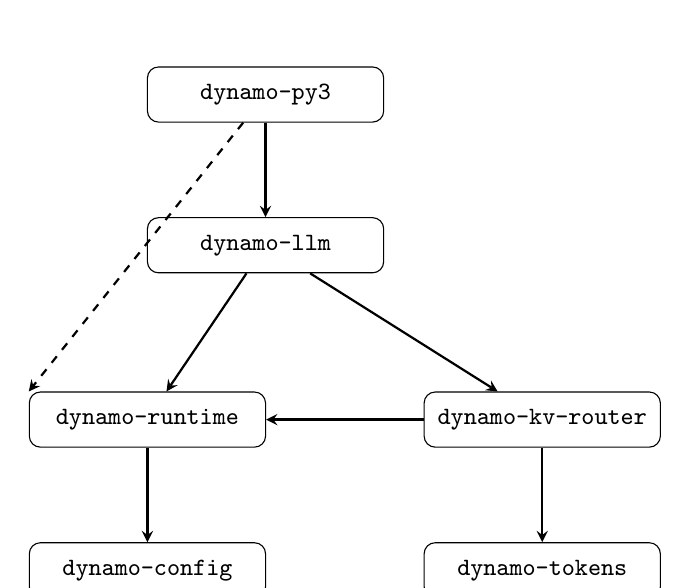
\begin{tikzpicture}[
    node distance=1.2cm,
    crate/.style={rectangle, draw, rounded corners, minimum width=3cm, minimum height=0.7cm, align=center, font=\small},
    arrow/.style={->, thick, >=stealth}
]
  % Bottom layer
  \node[crate] (config) {\texttt{dynamo-config}};
  \node[crate, right=2cm of config] (tokens) {\texttt{dynamo-tokens}};

  % Middle layer
  \node[crate, above=of config] (runtime) {\texttt{dynamo-runtime}};
  \node[crate, right=2cm of runtime] (kvrouter) {\texttt{dynamo-kv-router}};

  % Upper layer
  \node[crate, above=1.5cm of runtime, xshift=1.5cm] (llm) {\texttt{dynamo-llm}};

  % Top layer
  \node[crate, above=of llm] (py3) {\texttt{dynamo-py3}};

  % Arrows
  \draw[arrow] (runtime) -- (config);
  \draw[arrow] (kvrouter) -- (runtime);
  \draw[arrow] (kvrouter) -- (tokens);
  \draw[arrow] (llm) -- (runtime);
  \draw[arrow] (llm) -- (kvrouter);
  \draw[arrow] (py3) -- (llm.north);
  \draw[arrow, dashed] (py3) -- (runtime.north west);
\end{tikzpicture}
\end{center}

\texttt{dynamo-config} sits at the base, providing configuration to all crates. \texttt{dynamo-runtime} builds on it with the distributed runtime (discovery, transports, pipeline framework). \texttt{dynamo-kv-router} depends on the runtime for communication and on \texttt{dynamo-tokens} for block hashing. \texttt{dynamo-llm} integrates everything: it depends on the runtime, the KV router, the token crate, the memory crate, and the parser crate. Finally, \texttt{dynamo-py3} sits at the top, exposing \texttt{dynamo-llm} and \texttt{dynamo-runtime} to Python.

%% ============================================================
\section{Summary}
\label{sec:architecture:summary}
%% ============================================================

\begin{itemize}
  \item A request's journey through Dynamo touches six stages: \textbf{HTTP ingress} (axum frontend), \textbf{preprocessing} (chat template + tokenization), \textbf{routing} (KV-aware worker selection), \textbf{dispatch} (TCP/NATS/HTTP transport), \textbf{inference} (vLLM/SGLang/TRT-LLM), and \textbf{streaming} (SSE output with per-token lifecycle management).

  \item \textbf{Service discovery} is pluggable, with backends for etcd/NATS JetStream KV stores and Kubernetes. The \texttt{Discovery} trait provides \texttt{list\_and\_watch} semantics that enable reactive fleet updates without restarts.

  \item Three \textbf{communication planes}---request (NATS/TCP/HTTP), event (NATS Core/ZMQ), and GPU data (NIXL/NCCL)---serve different performance and reliability profiles. Each is chosen to match its data type.

  \item The \textbf{PyO3 bridge} separates Rust (data plane) from Python (control plane), crossing the boundary per-request with lightweight serialization. The GIL is held only during brief object conversion, not during GPU computation.

  \item Dynamo's \textbf{crate architecture} is layered: \texttt{dynamo-config} $\rightarrow$ \texttt{dynamo-runtime} $\rightarrow$ \texttt{dynamo-kv-router} / \texttt{dynamo-tokens} $\rightarrow$ \texttt{dynamo-llm} $\rightarrow$ \texttt{dynamo-py3}. Each layer has a well-defined responsibility boundary.

  \item Dynamo is a \textbf{polyglot system}: Rust, Python, Go, and C++ each handle the components best suited to their strengths, with integration complexity concentrated at language boundaries.
\end{itemize}

\medskip
\begin{center}\rule{0.5\linewidth}{0.4pt}\end{center}
\medskip

With the architecture mapped, we can now zoom into the component that makes Dynamo's routing unique: the KV-aware radix tree that decides which GPU should handle each request.

\medskip
\noindent\textbf{Check Your Understanding}

\smallskip
\noindent\emph{These questions are answerable from this chapter alone.}

\begin{enumerate}
  \item Trace a request through Dynamo from HTTP ingress to the first generated token. Name every component and crate it touches, and identify which are Rust and which are Python.

  \item Why does Dynamo propagate all requests internally as streaming, even when the client requests \texttt{stream=false}? What design benefit does this provide?

  \item Explain the three communication planes (request, event, GPU data). For each, name the transport options and the type of data it carries. Why would using a single transport for all three be suboptimal?

  \item What happens when a GPU worker crashes unexpectedly? Trace the sequence of events through the etcd lease system, the discovery plane, and the router's radix tree.

  \item In a disaggregated configuration, the request touches two different GPU workers (prefill and decode). What data must be transferred between them, what protocol is used, and why is CPU involvement avoided?

  \item Describe the role of the \texttt{PythonAsyncEngine}. When is the GIL acquired and released during token generation? Why is GIL contention not a bottleneck for inference throughput?

  \item The \texttt{Discovery} trait has both a \texttt{list()} method and a \texttt{list\_and\_watch()} method. Why are both needed? In what scenarios would you use each?

  \item Look at the crate dependency graph. Why does \texttt{dynamo-kv-router} depend on \texttt{dynamo-tokens} but not on \texttt{dynamo-llm}? What architectural principle does this reflect?
\end{enumerate}

\medskip
\noindent\textbf{Answers}

\medskip

\begin{enumerate}
  \item The request enters the \textbf{axum HTTP frontend} (\texttt{dynamo-llm}, Rust), which validates JSON and checks model registration. It passes to the \textbf{preprocessor} (\texttt{dynamo-llm}, Rust: minijinja for chat templates, HF tokenizers for tokenization). The token sequence goes to the \textbf{router} (\texttt{dynamo-kv-router} for radix tree lookup, \texttt{dynamo-tokens} for block hashing, both Rust). The router dispatches via the \textbf{transport layer} (\texttt{dynamo-runtime}, Rust: TCP/NATS). The worker receives the request and invokes the \textbf{inference engine} (Python: vLLM/SGLang/TRT-LLM) via \texttt{PythonAsyncEngine} (PyO3 bridge in \texttt{dynamo-py3}, Rust$\leftrightarrow$Python). The first token streams back through the transport to the frontend.

  \item By treating all requests as streaming internally, the entire downstream pipeline handles a single pattern (async stream of token fragments). This eliminates duplicate code paths for streaming vs.\ non-streaming, reducing complexity and the associated bug surface. Non-streaming responses are simply the aggregation of a complete stream at the frontend boundary.

  \item \textbf{Request plane}: NATS, TCP (TwoPartCodec), or HTTP/2; carries inference requests and responses; optimized for low-latency point-to-point communication. \textbf{Event plane}: NATS Core or ZMQ; carries KV cache events and metrics; optimized for async fan-out pub/sub. \textbf{GPU data plane}: NIXL (RDMA) or NCCL; carries KV cache blocks and all-reduce tensors; optimized for maximal bandwidth with zero CPU involvement. A single transport would force a compromise: pub/sub systems add routing overhead to the request path, point-to-point TCP cannot do fan-out efficiently, and neither can move GPU memory without CPU copies.

  \item When a worker crashes: (1) its etcd lease keep-alive stops; (2) after the TTL expires, etcd deletes all keys associated with the lease; (3) the router's \texttt{list\_and\_watch} stream emits a \texttt{DiscoveryEvent::Removed}; (4) the router removes the worker from its routing table; (5) all entries for that worker's ID are evicted from the radix tree; (6) subsequent requests are routed only to remaining healthy workers. Any in-flight requests to the crashed worker will time out and may be retried.

  \item The prefill worker computes the \textbf{KV cache} (key and value tensors for all layers and all input tokens). This cache is transferred to the decode worker via \textbf{NIXL}, which performs direct GPU-to-GPU memory transfer using RDMA. CPU involvement is avoided because the KV cache is large (gigabytes for long contexts) and copying it through CPU memory would add unacceptable latency and consume PCIe bandwidth that the GPU needs for inference.

  \item \texttt{PythonAsyncEngine} implements Rust's \texttt{AsyncEngine} trait by wrapping a Python async generator. The GIL is acquired briefly to (a) call the Python generator function and (b) convert each yielded Python object to Rust types via \texttt{depythonize}. Between yield points---while the GPU is executing inference kernels---the GIL is \emph{released}. GIL contention is not a bottleneck because GPU kernel execution (the dominant cost) happens in C++/CUDA land outside the GIL, and the conversion overhead is microseconds compared to milliseconds of GPU computation per token.

  \item \texttt{list()} returns a one-time snapshot, useful at startup to bootstrap the routing table with all currently registered workers. \texttt{list\_and\_watch()} returns a continuous stream of add/remove events, used by long-running components (routers, frontends) to react to fleet changes in real time. Using only \texttt{list()} would miss dynamic changes; using only \texttt{list\_and\_watch()} would miss instances that registered before the watch started (race condition).

  \item \texttt{dynamo-kv-router} depends on \texttt{dynamo-tokens} because it needs block hash computation to map token sequences to radix tree entries. It does \emph{not} depend on \texttt{dynamo-llm} because the router's indexing logic is model-agnostic---it operates on abstract block hashes and worker IDs, not on model-specific types. This reflects the \textbf{dependency inversion principle}: the high-level orchestration crate (\texttt{dynamo-llm}) depends on the low-level algorithmic crate (\texttt{dynamo-kv-router}), not the reverse. This keeps the router testable and reusable independently of any specific inference engine.
\end{enumerate}

\chapter{KV-Aware Routing and the Radix Tree}
\label{ch:kvrouter}

When a request arrives at Dynamo's router, it must answer a deceptively simple question: \emph{which GPU should handle this request?} A naive round-robin or least-loaded strategy ignores the most valuable information available---which GPU already has relevant KV cache blocks in memory. Routing a request to a GPU that has already cached 90\% of the prompt's KV data saves the compute cost of prefill for those tokens, reduces time to first token, and avoids wasting memory on duplicate cache entries. This chapter explains how Dynamo makes this decision, building from the foundational data structure (the radix tree) through the hashing scheme, cost function, and concurrency strategy.

\section{The Routing Problem}
\label{sec:kvrouter:problem}

\marginnote{\emph{Cache hit rate:} the fraction of a request's token blocks already present in the target worker's KV cache.}%
Consider a fleet of $W$ GPU workers serving an LLM. Each worker maintains a KV cache---a memory region storing the key and value tensors computed during previous requests' prefill phases. When a new request arrives with token sequence $[t_1, t_2, \ldots, t_n]$, the router must choose one of the $W$ workers. If the chosen worker already has KV cache entries for a prefix $[t_1, \ldots, t_k]$ of the request (from a prior request that shared the same system prompt, for instance), then only tokens $[t_{k+1}, \ldots, t_n]$ need prefill computation. The savings are proportional to $k/n$.

The routing problem is a multi-objective optimization. The router must balance three competing goals:

\begin{enumerate}
  \item \textbf{Maximize KV cache reuse.} Route to the worker with the most relevant cached blocks. This minimizes prefill computation and time to first token.
  \item \textbf{Balance load across workers.} Avoid overloading any single GPU. A worker with perfect cache overlap but a queue of 50 pending requests may be slower than a worker with zero cache overlap and an empty queue.
  \item \textbf{Minimize latency.} Prefer workers that can start processing immediately, accounting for both cache benefit and queueing delay.
\end{enumerate}

These goals conflict: the worker with the best cache hit rate may also be the most heavily loaded. In production, many requests share the same system prompt, so without a load-balancing counterweight, all such requests would route to the same worker---creating a hotspot.

\begin{insightbox}
The routing problem reduces to a \emph{prefix matching} problem: given a new request's token blocks, find which workers have cached the longest matching prefix. The data structure that makes this efficient---the radix tree---is the subject of the next section.
\end{insightbox}

\begin{whynotbox}{Why not just use a hash table mapping requests to workers?}
A simpler design would hash the entire prompt and look up which worker last served an identical prompt. This fails for two reasons.

\textbf{Prefix sharing.} Two requests that share a 2000-token system prompt but differ in their 50-token user messages have completely different full-prompt hashes---yet 97.5\% of their KV cache is identical. A hash table sees them as unrelated; a prefix-matching structure recognizes the overlap.

\textbf{Partial reuse.} Even when no worker has the \emph{complete} prefix cached, one worker may have 80\% of it. A hash table returns ``miss'' for anything less than an exact match. The radix tree returns the overlap \emph{depth} for every worker, enabling the cost function to make a graded decision.
\end{whynotbox}

Dynamo resolves the tension between cache affinity and load balancing through a \emph{cost function} that combines cache overlap with load metrics into a single scalar score per worker. The router evaluates this function for every candidate worker and selects the one with the best score. The configurable weight between these two factors is the \texttt{overlap\_score\_weight} parameter in \texttt{KvRouterConfig}, which defaults to \texttt{1.0}. Setting it to zero disables cache-aware routing entirely, reducing the router to a pure load balancer.

\section{Tries and Radix Trees}
\label{sec:kvrouter:trie}

\marginnote{\emph{Trie:} a tree where each node represents a single element of a key, and paths from root to leaf spell out complete keys.}%
A \emph{trie} (from ``retrieval'') is a tree-shaped data structure for storing and looking up sequences. Each node in a trie represents a single element---in our case, a single block hash. A path from the root to any node spells out a prefix of some stored sequence. Tries support efficient prefix matching: to find all sequences that share a given prefix, we simply walk the tree following the prefix elements. The lookup cost is $O(k)$ where $k$ is the length of the prefix, independent of the number of stored sequences.

A \emph{radix tree} (also called a \emph{Patricia trie} or \emph{compressed trie}) optimizes the trie by merging chains of single-child nodes into single edges that carry multiple elements. If a trie has a chain of nodes $A \to B \to C$ where $B$ has only one child, the radix tree collapses this into a single edge $A \to C$ labeled with both elements. This compression reduces memory usage and speeds up traversal for keys with long unique suffixes---exactly the pattern that arises in LLM serving, where many requests share a long system prompt prefix and diverge only in the user message.

To make this concrete: consider a chat application where every request begins with a 2000-token system prompt (about 125 blocks at block size 16), followed by a user message. In a plain trie, the shared prefix creates a chain of 125 single-child nodes that every lookup must traverse. In a radix tree, this chain collapses into a single edge, and the tree branches only where user messages diverge. The memory savings and traversal speedup are proportional to the length of the shared prefix.

Figure~\ref{fig:radix-tree-example} illustrates this structure with a concrete example.

\begin{figure}[ht]
\centering
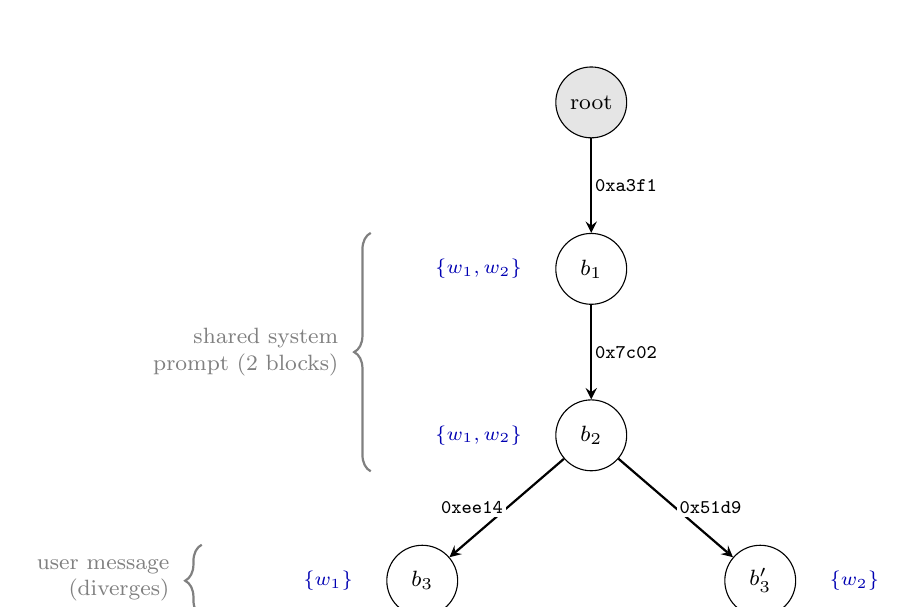
\begin{tikzpicture}[
    node distance=1.2cm and 2.2cm,
    treenode/.style={circle, draw, minimum size=0.9cm, font=\footnotesize, inner sep=1pt},
    rootnode/.style={treenode, fill=gray!20},
    edge label/.style={font=\scriptsize, midway, fill=white, inner sep=1pt},
    workerset/.style={font=\scriptsize\ttfamily, text=blue!70!black},
    arrow/.style={->, >=stealth, thick},
]
    % Root
    \node[rootnode] (root) {root};

    % Level 1: shared system prompt block
    \node[treenode, below=1.2cm of root] (b1) {$b_1$};
    \draw[arrow] (root) -- node[edge label, right] {\texttt{0xa3f1}} (b1);
    \node[workerset, left=0.3cm of b1] {$\{w_1, w_2\}$};

    % Level 2: shared system prompt block
    \node[treenode, below=1.2cm of b1] (b2) {$b_2$};
    \draw[arrow] (b1) -- node[edge label, right] {\texttt{0x7c02}} (b2);
    \node[workerset, left=0.3cm of b2] {$\{w_1, w_2\}$};

    % Level 3: divergence — two different user messages
    \node[treenode, below left=1.2cm and 1.5cm of b2] (b3a) {$b_3$};
    \node[treenode, below right=1.2cm and 1.5cm of b2] (b3b) {$b_3'$};

    \draw[arrow] (b2) -- node[edge label, left] {\texttt{0xee14}} (b3a);
    \draw[arrow] (b2) -- node[edge label, right] {\texttt{0x51d9}} (b3b);

    \node[workerset, left=0.3cm of b3a] {$\{w_1\}$};
    \node[workerset, right=0.3cm of b3b] {$\{w_2\}$};

    % Annotations
    \draw[decorate, decoration={brace, amplitude=6pt, mirror}, thick, gray]
        ([xshift=-2.8cm]b1.north) -- ([xshift=-2.8cm]b2.south)
        node[midway, left=8pt, font=\footnotesize, align=right, text=gray] {shared system\\prompt (2 blocks)};
    \draw[decorate, decoration={brace, amplitude=6pt, mirror}, thick, gray]
        ([xshift=-2.8cm]b3a.north) -- ([xshift=-2.8cm]b3a.south)
        node[midway, left=8pt, font=\footnotesize, align=right, text=gray] {user message\\(diverges)};
\end{tikzpicture}
\caption{A radix tree with two requests sharing a two-block system prompt prefix. Edge labels are \texttt{LocalBlockHash} values (truncated for readability). Worker sets at each node show which GPUs have that block cached. Workers $w_1$ and $w_2$ both cache the shared prefix ($b_1$, $b_2$); they diverge at the user message, where $w_1$ cached one user's query ($b_3$, hash \texttt{0xee14}) and $w_2$ cached another ($b_3'$, hash \texttt{0x51d9}). A new request with the same system prompt but a third user message would match both workers for depth~2, and neither for depth~3.}
\label{fig:radix-tree-example}
\end{figure}

Note that Dynamo's \texttt{RadixTree} does not perform explicit edge compression in its data structure---each \texttt{RadixBlock} node corresponds to a single block hash. The ``radix tree'' behavior emerges implicitly: when a node has only one child, the tree effectively stores a single-element edge, and the traversal simply follows the single child pointer. True compression (storing multiple hashes on a single edge) would complicate insertion and deletion logic for a marginal performance gain.

\subsection{Dynamo's Node Structure}

In Dynamo's \texttt{RadixTree}, each node is a \texttt{RadixBlock}:

\begin{verbatim}
pub(crate) struct RadixBlock {
    pub(crate) children:
        FxHashMap<LocalBlockHash, SharedRadixBlock>,
    pub(crate) workers: FxHashSet<WorkerWithDpRank>,
    pub(crate) block_hash:
        Option<ExternalSequenceBlockHash>,
    pub(crate) recent_uses: VecDeque<Instant>,
}
\end{verbatim}

Four fields serve four purposes:

\begin{itemize}
  \item \textbf{\texttt{children}}: A hash map from \texttt{LocalBlockHash} to child nodes. Each child represents the next block in a stored sequence. The use of \texttt{FxHashMap} (a fast, non-cryptographic hash map from the \texttt{rustc-hash} crate) optimizes for the common case of small maps with integer keys.
  \item \textbf{\texttt{workers}}: The set of workers that have this block cached. When we traverse the tree during \texttt{find\_matches}, this set tells us which workers can reuse this block's KV cache. Workers are identified by \texttt{WorkerWithDpRank}, a struct combining a \texttt{WorkerId} (a \texttt{u64}) with a data-parallel rank.
  \item \textbf{\texttt{block\_hash}}: The external sequence block hash---a position-aware hash that incorporates the block's ancestry. This is \texttt{None} for the root node and \texttt{Some(...)} for all others.
  \item \textbf{\texttt{recent\_uses}}: A time-ordered buffer of recent accesses, used for frequency-based routing when \texttt{expiration\_duration} is configured. This enables the router to prefer ``hot'' prefixes over stale ones.
\end{itemize}

The tree itself stores a root node and a per-worker lookup table:

\begin{verbatim}
pub struct RadixTree {
    pub(crate) root: SharedRadixBlock,
    pub(crate) lookup: FxHashMap<
        WorkerWithDpRank,
        FxHashMap<ExternalSequenceBlockHash,
                  SharedRadixBlock>>,
    pub(crate) expiration_duration: Option<Duration>,
}
\end{verbatim}

\marginnote{\texttt{Shared\-Radix\-Block} is \texttt{Rc<Ref\-Cell<\-Radix\-Block>{}>}---a reference-counted pointer with runtime borrow checking.}%
The \texttt{lookup} table provides $O(1)$ access to any block by worker and sequence hash, bypassing the need to traverse the tree from the root. This is essential for \texttt{apply\_event} operations, where a store event specifies a parent hash and needs to find the parent block directly.

\begin{notebox}
The \texttt{lookup} table serves a dual purpose: it enables $O(1)$ block access for event processing, and it provides tree size information per worker. The \texttt{tree\_sizes} field in \texttt{OverlapScores} is populated from \texttt{lookup.get(worker).len()}, giving the router a signal about how much data each worker has cached overall---used as a tie-breaker when multiple workers have identical overlap scores.
\end{notebox}

\section{Block Hashing}
\label{sec:kvrouter:hashing}

Before the radix tree can store or look up a request's tokens, the token sequence must be converted into a sequence of block hashes. This conversion is a two-step process:

\begin{enumerate}
  \item \textbf{Partition into blocks.} The token sequence is divided into fixed-size blocks of $B$ tokens (typically $B = 16$ or $B = 32$). The function \texttt{compute\_block\_hash\_for\_seq} uses \texttt{chunks\_exact(kv\_block\_size as usize)}, meaning only complete blocks are hashed---any trailing partial block is discarded. This is correct because only complete blocks can be cached and reused.
  \item \textbf{Hash with XXH3.} Each block is hashed using XXH3 (a fast, non-cryptographic hash function from the \texttt{xxhash-rust} crate) with seed \texttt{1337}. The input bytes are the little-endian encoding of the token IDs in the block.
\end{enumerate}

This produces a \texttt{LocalBlockHash}---a \texttt{u64} that identifies the \emph{content} of a block:

\begin{verbatim}
pub struct LocalBlockHash(pub u64);
\end{verbatim}

\subsection{Sequence Hashes: Encoding Position}

\marginnote{\emph{Positional hashing:} incorporating sequence position into the block hash to distinguish otherwise-identical blocks at different positions.}%
A \texttt{LocalBlockHash} captures \emph{what} tokens are in a block, but not \emph{where} the block appears in the sequence. This distinction matters because the KV cache values depend on position---via RoPE (Rotary Position Embedding) or other positional encodings. Two blocks with identical tokens at positions 0 and 100 produce different KV cache entries and must not be confused.

Dynamo solves this with \texttt{ExternalSequenceBlockHash}, a rolling hash that chains each block to its parent:

\begin{verbatim}
pub struct ExternalSequenceBlockHash(pub u64);
\end{verbatim}

The computation is defined in \texttt{compute\_seq\_hash\_for\_block}:

\begin{verbatim}
// First block: seq_hash = local_hash
sequence_hashes.push(block_hashes[0].0);

// Subsequent blocks:
// seq_hash = XXH3([parent_seq_hash, current_local_hash])
for i in 1..block_hashes.len() {
    let combined = [sequence_hashes[i-1],
                    block_hashes[i].0];
    let bytes: Vec<u8> = combined.iter()
        .flat_map(|&num| num.to_le_bytes())
        .collect();
    let seq_hash = compute_hash(&bytes);
    sequence_hashes.push(seq_hash);
}
\end{verbatim}

The first block's sequence hash equals its local hash (it has no parent). Each subsequent block's sequence hash is \texttt{XXH3(parent\_seq\_hash || local\_hash)}. This creates a chain: the sequence hash at position $i$ depends on every block from position 0 through $i$. Two sequences that share a common prefix of length $k$ blocks will have identical sequence hashes for blocks $0$ through $k-1$ and divergent hashes from block $k$ onward.

\begin{insightbox}
The radix tree uses \texttt{LocalBlockHash} as keys in the \texttt{children} map (for tree traversal), and \texttt{ExternalSequenceBlockHash} as keys in the \texttt{lookup} table (for direct block access). This two-hash design separates the concerns of tree navigation (content-based) and block identification (position-aware).
\end{insightbox}

\subsection{LoRA and Multimodal Hashing}

The hash computation can incorporate additional context beyond raw tokens. When a LoRA adapter name is provided, it is mixed into the XXH3 seed:

\begin{verbatim}
let seed = match lora_name.filter(|n| !n.is_empty()) {
    Some(name) =>
        XXH3_SEED.wrapping_add(xxh3::xxh3_64(name.as_bytes())),
    None => XXH3_SEED,
};
\end{verbatim}

This ensures that blocks cached under different LoRA adapters produce distinct hashes---the same tokens processed by adapter A and adapter B yield different KV cache entries and must not be conflated. Similarly, when multimodal metadata is present (image embeddings, for instance), the multimodal object hashes are appended to the token bytes before hashing, ensuring that blocks with identical tokens but different images produce different block hashes.

\subsection{Lazy Hash Computation}

Hash computation is not free---for a 4096-token prompt with block size 32, computing 128 block hashes involves 128 XXH3 invocations, plus 128 more for the rolling sequence hashes. To avoid paying this cost when it is not needed, Dynamo wraps tokens in a \texttt{TokensWithHashes} struct that computes hashes lazily:

\begin{verbatim}
pub struct TokensWithHashes {
    tokens: Vec<u32>,
    block_size: u32,
    block_hashes: Option<Vec<LocalBlockHash>>,
    seq_hashes: Option<Vec<SequenceHash>>,
    // ... additional fields
}
\end{verbatim}

The \texttt{get\_or\_compute\_block\_hashes()} method computes block hashes on first call and caches the result. The \texttt{get\_or\_compute\_seq\_hashes()} method first ensures block hashes are computed (since sequence hashes depend on them), then computes and caches the rolling sequence hashes. If the routing decision path calls \texttt{find\_matches} and then later needs to record the routing decision (which requires sequence hashes), the block hashes computed for the first call are reused---avoiding redundant work.

With hashing in place, we can now turn to how the router \emph{uses} these hashes: given a sequence of block hashes for a new request, how does the radix tree produce a per-worker overlap score, and how does the cost function convert those scores into a routing decision?

\section{The Routing Cost Function}
\label{sec:kvrouter:cost}

The \texttt{find\_matches} method on \texttt{RadixTree} walks the tree along the request's block hash sequence and produces an \texttt{OverlapScores} struct:

\begin{verbatim}
pub struct OverlapScores {
    pub scores: FxHashMap<WorkerWithDpRank, u32>,
    pub frequencies: Vec<usize>,
    pub tree_sizes: FxHashMap<WorkerWithDpRank, usize>,
}
\end{verbatim}

The \texttt{scores} map records, for each worker, the number of consecutive prefix blocks that worker has cached. This is the \emph{overlap depth}: if worker $w$ has cached blocks 0 through 49 of a 100-block request, its overlap score is 50.

\subsection{The Traversal Algorithm}

The traversal maintains an \emph{active set} of workers. Starting from the root, it looks up the first block hash in the root's children. The workers at that child node form the initial active set. As traversal proceeds through the sequence:

\begin{itemize}
  \item If a child node has \emph{fewer} workers than the active set, workers have ``dropped out''---they do not have this block cached. The algorithm records their scores (the depth at which they dropped) and shrinks the active set.
  \item If a child node has \emph{more} workers than the active set, this indicates stale entries---workers whose ancestor remove events have arrived but whose descendant remove events have not yet propagated. The code handles this with a full membership check, retaining only workers present in both sets.
  \item If the active set has exactly one worker remaining and \texttt{early\_exit} is true, the algorithm stops---there is only one candidate, and further traversal cannot change the decision.
\end{itemize}

Workers that survive to the deepest matched level receive the maximum score. This traversal is $O(k)$ in the number of blocks $k$, with each step performing a hash map lookup and a set intersection.

\begin{notebox}
The \texttt{early\_exit} optimization reflects a design trade-off: when only one worker matches any prefix at all, there is no benefit to determining the exact overlap depth---the router will select that worker regardless. By stopping early, the router reduces latency on the critical path. The \texttt{early\_exit} flag is set to \texttt{true} when the routing decision only needs a single candidate, not a complete ranking.
\end{notebox}

\subsection{Event Processing: Building and Maintaining the Tree}

The radix tree is not built from a static dataset---it is maintained incrementally as workers report cache events. The \texttt{apply\_event} method processes three kinds of events, each represented by a variant of \texttt{KvCacheEventData}:

\textbf{Stored events.} When a worker finishes prefilling a request, it reports which blocks were stored. The event contains a \texttt{parent\_hash} (the sequence hash of the block after which the new blocks follow, or \texttt{None} if they start from the root) and a list of \texttt{KvCacheStoredBlockData} entries, each containing a \texttt{block\_hash} (sequence hash), a \texttt{tokens\_hash} (local hash), and optional multimodal metadata. The algorithm:

\begin{enumerate}
  \item Looks up the parent block in the worker's \texttt{lookup} table (or uses the root if \texttt{parent\_hash} is \texttt{None}).
  \item For each block in the event, borrows the parent mutably, inserts the worker into the parent's \texttt{workers} set, then looks up or creates the child in the parent's \texttt{children} map.
  \item Registers the new block in the worker's \texttt{lookup} table for future $O(1)$ access.
\end{enumerate}

A key subtlety: the algorithm uses a ``deferred insert'' pattern to avoid double-borrowing. It holds a mutable borrow on the parent to insert the child, but the worker insertion into the \emph{child's} worker set is deferred to the next iteration, when the child becomes the new parent. This hand-over-hand borrowing is what makes the self-reference bug (Bug~\#2) possible when the child \texttt{Rc} aliases the parent.

\textbf{Removed events.} When a worker evicts blocks from its KV cache, it reports the sequence hashes of the evicted blocks. The algorithm looks up each block hash in the worker's \texttt{lookup} table, removes the worker from the block's \texttt{workers} set, and if the set becomes empty, clears the block's children (since no worker has any descendant blocks cached either). Importantly, removal does \emph{not} cascade to descendant blocks---each block is removed individually. This means the tree may transiently contain ``stale'' entries where a child block lists a worker that its parent does not. The \texttt{find\_matches} traversal handles this gracefully via the \texttt{child\_count > active\_count} branch.

\textbf{Cleared events.} When a worker restarts or loses all its cache, it sends a cleared event. This removes the worker from every block it had registered, but keeps the worker tracked in the \texttt{lookup} table (with an empty map) so the router knows the worker exists and can route new requests to it.

The traversal and event-processing algorithms described above assume exclusive access to the tree---but in a production router, reads (\texttt{find\_matches}) and writes (\texttt{apply\_event}) may arrive concurrently. The next section examines how Dynamo handles this with three different concurrency strategies.

\section{Concurrency: \texttt{Rc<RefCell>} vs \texttt{Arc<RwLock>}}
\label{sec:kvrouter:concurrency}

\marginnote{\emph{Interior mutability:} mutating data through a shared reference, checked at runtime rather than compile time.}%
The radix tree is a shared, mutable data structure: routing decisions read from it, while cache updates (insertions, evictions) write to it. Dynamo provides \emph{three} implementations of the indexer, each with different concurrency properties.

\subsection{RadixTree: Single-Threaded with Rc<RefCell>}

The original implementation uses \texttt{Rc<RefCell<RadixBlock>{}>} for nodes---reference-counted pointers with runtime borrow checking. \texttt{Rc} (Reference Counted) is Rust's single-threaded shared ownership type: it tracks how many pointers reference a value and frees the value when the count reaches zero. \texttt{RefCell} provides interior mutability by enforcing the borrowing rules at runtime instead of compile time.

\begin{verbatim}
pub(crate) type SharedRadixBlock = Rc<RefCell<RadixBlock>>;
\end{verbatim}

This is a single-threaded design: \texttt{Rc} does not implement the \texttt{Send} or \texttt{Sync} traits, so the Rust compiler physically prevents the tree from being shared across threads. All operations---event processing and match requests---run on a single thread in an async event loop.

The advantage is zero synchronization overhead. Every pointer traversal is a simple reference count increment (no atomic operations), and every borrow check is a cheap comparison of a cell-local counter. The disadvantage is that read operations (\texttt{find\_matches}) and write operations (\texttt{apply\_event}) cannot overlap---the single thread must serialize them. For small-to-medium deployments where the routing decision latency is dominated by network I/O rather than tree traversal, this is acceptable. For high-throughput deployments with hundreds of workers and thousands of concurrent requests, the serialization becomes a bottleneck.

\begin{bugbox}
The \texttt{Rc<RefCell>} design has a subtle failure mode discovered by our fuzzing campaign. During \texttt{apply\_event}, the algorithm traverses from parent to child, holding a mutable borrow on the parent (\texttt{parent\_mut = current.borrow\_mut()}) while looking up the child in \texttt{parent\_mut.children}. If a hash collision causes a node to be inserted as its own child---that is, the child \texttt{Rc} points to the same allocation as the parent---the subsequent \texttt{child.borrow\_mut()} panics because the parent's \texttt{RefCell} is already mutably borrowed. This is Bug~\#2 in Chapter~\ref{ch:findings}: a self-referencing block causing a \texttt{RefCell} panic (or a deadlock in the concurrent variant).

The fix was a runtime guard using \texttt{try\_borrow\_mut}:
\begin{verbatim}
if child.try_borrow_mut().is_err() {
    tracing::warn!(
        "Detected self referencing block; \
         rejecting sequence"
    );
    return Err(
        KvCacheEventError::InvalidBlockSequence);
}
\end{verbatim}
This converts the panic into a graceful error return, but the underlying issue---that the \texttt{lookup} table can alias a block back to itself---remains a structural property of the design.
\end{bugbox}

\begin{whynotbox}{Why \texttt{Rc<RefCell>} instead of \texttt{Arc<RwLock>} by default?}
If the concurrent variant exists, why not use it everywhere and avoid the single-threaded limitation?

\textbf{Cost of atomics.} Every \texttt{Arc::clone()} performs an atomic increment---roughly 5--20$\times$ slower than \texttt{Rc::clone()}'s non-atomic increment on modern x86 hardware. During \texttt{find\_matches}, the traversal clones a shared pointer at every level of the tree. For a 200-block prefix, that is 200 atomic operations per routing decision. At 1000 requests per second, this adds up to 200{,}000 unnecessary atomic operations per second when all work runs on a single async thread anyway.

\textbf{Lock overhead.} Each \texttt{RwLock::read()} acquires a reader lock, even when no writer is present. The \texttt{parking\_lot} implementation is fast (a single atomic compare-and-swap in the uncontended case), but \texttt{RefCell::borrow()} is faster still---a non-atomic comparison of a cell-local counter.

\textbf{The design philosophy.} Dynamo defaults to single-threaded operation (\texttt{router\_event\_threads = 1}) and only opts into the concurrent variant when the deployment scale justifies the overhead. This is Rust's zero-cost abstraction principle applied to data structure design: pay for concurrency only when you need it.
\end{whynotbox}

\subsection{ConcurrentRadixTree: Multi-Threaded with Arc<RwLock>}

The concurrent variant replaces every \texttt{Rc} with \texttt{Arc} (Atomic Reference Counting) and every \texttt{RefCell} with \texttt{RwLock} (Reader-Writer Lock):

\begin{verbatim}
pub type SharedBlock = Arc<RwLock<Block>>;
\end{verbatim}

\texttt{Arc} uses atomic operations for reference counting, making it safe to share across threads. \texttt{RwLock} (from the \texttt{parking\_lot} crate, which provides a faster implementation than the standard library's) allows multiple concurrent readers or a single exclusive writer. The tree node structure is nearly identical to \texttt{RadixBlock}, but without the \texttt{recent\_uses} field---frequency tracking is omitted to keep \texttt{find\_matches} fully read-only.

The concurrency model is:
\begin{itemize}
  \item Multiple \texttt{find\_matches} calls can run in parallel, each acquiring only read locks.
  \item Write operations (\texttt{apply\_event}, \texttt{remove\_worker}) acquire write locks.
  \item Deadlock prevention is ensured by always locking parent before child (hand-over-hand locking).
\end{itemize}

The configuration parameter \texttt{router\_event\_threads} (default: 4) controls which implementation is used. When set to 1, the single-threaded \texttt{RadixTree} is used. When greater than 1, the \texttt{ConcurrentRadixTree} with a thread pool handles events on $N$ worker threads while \texttt{find\_matches} runs inline on the caller's thread.

\begin{notebox}
Both the \texttt{RadixTree} and \texttt{ConcurrentRadixTree} implement a custom \texttt{Drop} to avoid stack overflow. A deeply nested tree dropped recursively would create a call stack proportional to the tree depth. Both implementations use an iterative approach: they drain children into a stack vector and drop them in a loop, converting $O(d)$ recursion depth into $O(1)$ stack usage.
\end{notebox}

\subsection{PositionalIndexer: A Flat Alternative}

The third implementation, \texttt{PositionalIndexer}, abandons the tree structure entirely. Instead of building a trie, it stores blocks in a flat \texttt{DashMap} keyed by \texttt{(position, LocalBlockHash)} pairs:

\begin{verbatim}
pub struct PositionalIndexer {
    index: DashMap<(usize, LocalBlockHash),
                   SeqEntry, FxBuildHasher>,
    tree_sizes: DashMap<WorkerWithDpRank,
                        AtomicUsize, FxBuildHasher>,
    jump_size: usize,
}
\end{verbatim}

Instead of traversing a tree, \texttt{find\_matches} performs a \emph{jump search}: it checks positions at intervals of \texttt{jump\_size} (e.g., 32), and only scans intermediate positions when workers drop out at a jump boundary. This exploits the observation that if a worker matches at position $p$ and also at position $p + 32$, it very likely matches at all intermediate positions (since blocks form a chain and eviction typically removes entire suffixes).

The jump search algorithm proceeds as follows:
\begin{enumerate}
  \item Initialize the active set from workers matching at position 0.
  \item Jump forward by \texttt{jump\_size} positions.
  \item If the same number of workers match at the destination: skip the intermediate positions and continue jumping (fast path).
  \item If fewer workers match: scan the intermediate range position-by-position to find the exact dropout points (slow path).
  \item Record final scores for workers that survive to the end.
\end{enumerate}

The worst-case complexity is still $O(k)$, but the average case is $O(k / \mathit{jump\_size})$ when prefixes are long and workers are stable---a significant speedup for prompts with thousands of blocks.

\begin{insightbox}
The \texttt{PositionalIndexer} also computes \texttt{ExternalSequenceBlockHash} lazily during \texttt{find\_matches}, using \texttt{ensure\_seq\_hash\_computed} to extend a vector of rolling hashes on demand. This avoids computing sequence hashes for positions beyond the first mismatch, saving work when the matching prefix is short.
\end{insightbox}

The \texttt{PositionalIndexer}'s innermost lookup uses a \texttt{SeqEntry} enum that optimizes for the common case:

\begin{verbatim}
enum SeqEntry {
    Single(ExternalSequenceBlockHash,
           FxHashSet<WorkerWithDpRank>),
    Multi(FxHashMap<ExternalSequenceBlockHash,
                    FxHashSet<WorkerWithDpRank>>),
}
\end{verbatim}

At a given \texttt{(position, local\_hash)} pair, there is typically only one sequence hash (the \texttt{Single} variant), because most blocks at a given position with a given content hash share the same ancestry. The \texttt{Multi} variant handles the rare case where different prefix paths lead to blocks with identical content at the same position but different ancestry---causing distinct sequence hashes. By avoiding a \texttt{HashMap} allocation in the common case, \texttt{SeqEntry} reduces memory overhead significantly for large trees.

\subsection{The SyncIndexer Trait}

All three implementations conform to the \texttt{SyncIndexer} trait, which provides a uniform interface for the thread pool infrastructure:

\begin{verbatim}
pub trait SyncIndexer: Send + Sync + 'static {
    fn worker(&self,
        event_receiver: flume::Receiver<WorkerTask>)
        -> anyhow::Result<()>;
    fn find_matches(&self,
        sequence: &[LocalBlockHash],
        early_exit: bool) -> OverlapScores;
}
\end{verbatim}

The \texttt{worker} method runs on a dedicated thread, processing events from a channel. The \texttt{find\_matches} method runs inline on the caller's thread---this is the key architectural insight. By keeping reads on the caller's thread and dispatching writes to worker threads, the system avoids channel overhead for the latency-sensitive read path while allowing writes to happen concurrently in the background. The higher-level \texttt{KvIndexerInterface} trait wraps \texttt{SyncIndexer} with async methods and Tokio channels for integration with the async runtime.

With the indexer providing overlap scores and the concurrency model ensuring those scores are computed safely, we can now examine the component that consumes them: the worker selector, which converts raw overlap scores into a final routing decision.

\section{The DefaultWorkerSelector}
\label{sec:kvrouter:selector}

\marginnote{\emph{ISL (Input Sequence Length):} the number of tokens in the request, used as a sizing signal.}%
The \texttt{DefaultWorkerSelector} is the concrete implementation that ties together the radix tree, cost function, and worker state. It implements the \texttt{WorkerSelector<C>} trait:

\begin{verbatim}
pub trait WorkerSelector<C: WorkerConfigLike> {
    fn select_worker(
        &self,
        workers: &HashMap<WorkerId, C>,
        request: &SchedulingRequest,
        block_size: u32,
    ) -> Result<WorkerSelectionResult, KvSchedulerError>;
}
\end{verbatim}

The generic parameter \texttt{C: WorkerConfigLike} abstracts over worker configuration, requiring methods \texttt{data\_parallel\_size()}, \texttt{data\_parallel\_start\_rank()}, \texttt{max\_num\_batched\_tokens()}, and \texttt{total\_kv\_blocks()}. This allows the selector to work with different backend configurations without coupling to any specific type.

The \texttt{SchedulingRequest} that arrives at the selector has already been enriched with information from multiple sources:

\begin{verbatim}
pub struct SchedulingRequest {
    pub isl_tokens: usize,
    pub overlaps: OverlapScores,
    pub decode_blocks: HashMap<WorkerWithDpRank, usize>,
    pub prefill_tokens: HashMap<WorkerWithDpRank, usize>,
    pub router_config_override: Option<RouterConfigOverride>,
    pub allowed_worker_ids: Option<HashSet<WorkerId>>,
    // ... additional fields
}
\end{verbatim}

The \texttt{overlaps} field comes from the indexer's \texttt{find\_matches}. The \texttt{decode\_blocks} and \texttt{prefill\_tokens} fields come from the active sequence tracker, which monitors in-flight requests. The optional \texttt{allowed\_worker\_ids} enables Endpoint Priority Policies (EPP) to restrict routing to a subset of workers.

\subsection{The Scoring Formula}

For each worker (and each of its data-parallel ranks), the selector computes a logit:

\begin{verbatim}
let logit = overlap_weight * potential_prefill_block
            + decode_block;
\end{verbatim}

This formula combines two signals:

\begin{itemize}
  \item \texttt{potential\_prefill\_block}: the number of blocks that would need to be prefilled, computed as \texttt{prefill\_tokens / block\_size}. When a worker has high cache overlap, this value is small (fewer blocks to compute), producing a lower logit. When overlap is zero, this equals the total request blocks.
  \item \texttt{decode\_block}: the number of active decode blocks on this worker---a measure of the worker's current load. Workers with more decode blocks are busier.
  \item \texttt{overlap\_weight}: the tunable parameter from \texttt{KvRouterConfig} (default: 1.0). Higher values prioritize cache reuse; lower values prioritize load balancing.
\end{itemize}

\begin{notebox}
The logit represents \emph{cost}, not benefit---lower is better. A worker with high cache overlap has fewer prefill blocks (lower first term), and a lightly loaded worker has fewer decode blocks (lower second term). The selector seeks the worker with the \emph{minimum} logit.
\end{notebox}

\subsection{Softmax Sampling}

Rather than deterministically selecting the minimum-logit worker, the selector uses \emph{softmax sampling} with a configurable temperature:

\begin{verbatim}
let candidates = softmax_sample(&worker_logits,
                                temperature);
\end{verbatim}

The \texttt{softmax\_sample} function normalizes the logits, negates them (since lower is better), scales by temperature, and samples from the resulting probability distribution. The temperature parameter controls exploration:

\begin{itemize}
  \item \texttt{temperature = 0.0} (default): deterministic selection. Returns the worker(s) with the minimum logit. If multiple workers are tied, returns all of them.
  \item \texttt{temperature > 0}: stochastic selection. Workers with lower logits are more likely to be selected, but any worker has a nonzero probability. Higher temperatures increase randomness.
\end{itemize}

When \texttt{temperature = 0.0} produces a tie (multiple workers with identical logits), the selector applies a \emph{tree size tie-breaker}: it selects the worker with the smallest tree size (fewest cached blocks overall). The intuition is that, among equally good workers for this request, the one with less total cache pressure is preferable. If tree sizes are also tied, the selection falls back to random.

\begin{whynotbox}{Why softmax sampling instead of always picking the best worker?}
With temperature 0 (the default), the selector \emph{does} pick the best worker deterministically. So why support nonzero temperature at all?

\textbf{Exploration.} A deterministic policy converges to a fixed routing pattern: the first worker to cache a popular prefix attracts all future requests for that prefix, and no other worker ever builds up cache for it. If that worker fails or becomes overloaded, the system has no fallback. Stochastic selection with a small temperature (e.g., 0.1) occasionally routes a request to a suboptimal worker, seeding cache entries that provide resilience.

\textbf{Fairness under skew.} In workloads with a power-law distribution of system prompts, the top-$k$ most popular prompts dominate traffic. Deterministic routing concentrates these on $k$ workers, leaving the rest underutilized. A small temperature spreads the load more evenly, at the cost of slightly lower cache hit rates.

\textbf{The softmax is cheap.} Computing $\exp(-\mathit{logit}_i / T)$ for $W$ workers involves $W$ exponentiations---negligible compared to the tree traversal or network round-trip. The flexibility costs almost nothing at runtime.
\end{whynotbox}

\subsection{The Complete Routing Path}

Putting it all together, the complete routing path for a new request is:

\begin{enumerate}
  \item The \texttt{SchedulingRequest} arrives with \texttt{isl\_tokens} (input sequence length), pre-computed \texttt{overlaps} (from the indexer's \texttt{find\_matches}), and per-worker \texttt{decode\_blocks} and \texttt{prefill\_tokens} from the active sequence tracker.
  \item The selector computes \texttt{request\_blocks = isl\_tokens.div\_ceil(block\_size)}.
  \item For each worker and data-parallel rank, it computes the logit using the formula above.
  \item Softmax sampling selects a candidate (or candidates, in the case of ties at temperature 0).
  \item Ties are broken by tree size, then randomly.
  \item The result is a \texttt{WorkerSelectionResult} containing the chosen \texttt{WorkerWithDpRank}, the number of required blocks, and the estimated overlap blocks.
\end{enumerate}

\begin{bugbox}
Step 2 contains a potential division-by-zero: \texttt{isl\_tokens.div\_ceil(block\_size as usize)} will panic if \texttt{block\_size} is zero. Our fuzzing campaign detected this as Bug~\#14 (Chapter~\ref{ch:findings}). In production, \texttt{block\_size} is set from the model configuration and is never zero, but the function does not validate its input. The same pattern---unchecked \texttt{div\_ceil} with an untrusted divisor---appeared in three other locations in the codebase.
\end{bugbox}

\subsection{Configuration and Tuning}

The \texttt{KvRouterConfig} struct centralizes all routing parameters. Beyond \texttt{overlap\_score\_weight} and \texttt{router\_temperature} (discussed above), several other parameters shape routing behavior:

\begin{itemize}
  \item \texttt{router\_track\_active\_blocks} (default: \texttt{true}): Whether to account for blocks from in-flight requests in the overlap calculation. When enabled, the router adds ``placeholder'' blocks for requests that are currently being processed, so a second request with the same prefix sees the first request's blocks as already claimed.
  \item \texttt{router\_assume\_kv\_reuse} (default: \texttt{true}): When tracking active blocks, whether to compute actual hash sequences (enabling cache-aware routing for in-flight requests) or use random hashes (assuming no reuse). Setting this to \texttt{false} saves hash computation at the cost of routing quality.
  \item \texttt{router\_ttl\_secs} (default: 120.0): When KV events are disabled, blocks expire from the tree after this duration. This prevents stale cache entries from influencing routing decisions indefinitely.
  \item \texttt{router\_max\_tree\_size} (default: $2^{20}$ = 1,048,576): The maximum number of blocks before pruning is triggered, preventing unbounded memory growth.
\end{itemize}

These parameters interact in subtle ways. For instance, \texttt{router\_assume\_kv\_reuse = true} with \texttt{overlap\_score\_weight = 0} wastes hash computation (computing hashes that are never used for scoring). The config validation catches some of these inconsistencies but not all---another area where fuzzing proved valuable by exercising unusual parameter combinations.

\section{Summary}

\begin{itemize}
  \item The \textbf{routing problem} balances KV cache reuse, load balancing, and latency minimization across a fleet of GPU workers. It reduces to prefix matching over block hash sequences.
  \item A \textbf{radix tree} stores block hashes with per-node worker sets, enabling efficient prefix overlap queries in $O(k)$ time. Each \texttt{RadixBlock} node contains a \texttt{children} map, a \texttt{workers} set, and an optional \texttt{block\_hash}.
  \item \textbf{Block hashing} uses XXH3 to convert token blocks into \texttt{LocalBlockHash} values. \textbf{Sequence hashing} chains blocks into position-aware \texttt{ExternalSequenceBlockHash} values using a rolling hash, ensuring identical tokens at different positions produce different hashes.
  \item The \textbf{cost function} computes a per-worker logit combining prefill cost (inversely related to cache overlap) and decode load, with a tunable \texttt{overlap\_score\_weight}. Selection uses softmax sampling with configurable temperature.
  \item \textbf{Three indexer implementations} serve different concurrency needs: \texttt{RadixTree} (\texttt{Rc<RefCell>}, single-threaded), \texttt{ConcurrentRadixTree} (\texttt{Arc<RwLock>}, multi-reader), and \texttt{PositionalIndexer} (flat \texttt{DashMap} with jump search, multi-threaded).
  \item The \texttt{Rc<RefCell>} design trades compile-time safety for runtime borrow checking---a category of bug detectable by fuzzing (Bug~\#2: self-referencing blocks causing \texttt{RefCell} panics or deadlocks).
  \item The \textbf{DefaultWorkerSelector} orchestrates the full routing decision, from overlap scores through softmax sampling to tree-size tie-breaking.
\end{itemize}

\medskip
\begin{center}\rule{0.5\linewidth}{0.4pt}\end{center}
\medskip

The router works in terms of block hashes, but where do those hashes come from? The next chapter explains how raw token sequences are partitioned into blocks, hashed with positional information, and managed through a type-state lifecycle.

\medskip
\noindent\textbf{Check Your Understanding}

\smallskip
\noindent\emph{These questions are answerable from this chapter alone.}

\begin{enumerate}
  \item Why is round-robin routing suboptimal for LLM inference? What information does it ignore?

  \textbf{Answer:} Round-robin ignores the KV cache state on each worker. If worker A has already cached the KV entries for a request's system prompt (from a prior request), routing to worker A allows those cached entries to be reused, skipping the expensive prefill computation for those tokens. Round-robin might send the request to worker B, which has no relevant cache entries, forcing a full prefill and wasting GPU compute.

  \item Explain the difference between a trie and a radix tree. Why does Dynamo use a radix tree rather than a plain trie?

  \textbf{Answer:} A trie stores one element per node, while a radix tree compresses chains of single-child nodes into single edges carrying multiple elements. Dynamo uses a radix tree because LLM requests often share long common prefixes (system prompts) followed by short unique suffixes (user messages). The radix tree compresses the shared prefix into fewer nodes, reducing memory usage and traversal time. In the extreme case where all requests share a 1000-block system prompt, a trie would have 1000 single-child nodes; a radix tree collapses them.

  \item Why must block hashing incorporate positional information? What would go wrong if two blocks with the same tokens at different positions produced the same hash?

  \textbf{Answer:} The KV cache values at a given position depend on that position (via RoPE or other positional encodings). If blocks at positions 0 and 100 with identical tokens produced the same hash, the router might reuse the KV cache from position 0 when processing position 100---producing incorrect attention scores and corrupted model output. The \texttt{ExternalSequenceBlockHash} rolling chain ensures that position information is encoded in every block's identity.

  \item The cost function balances cache overlap and load penalty. Describe a workload where pure cache-affinity routing would perform badly, and one where pure load balancing would perform badly.

  \textbf{Answer:} Pure cache-affinity performs badly when many requests share the same system prompt---all requests would route to the same worker (the one that first cached the prompt), creating a hotspot while other workers sit idle. Pure load balancing performs badly when requests have diverse, long prompts with significant overlap potential---it would distribute requests uniformly, preventing any worker from building up useful cache state, causing every request to pay the full prefill cost.

  \item Why does the \texttt{Rc<RefCell>} design create a risk of runtime panics that \texttt{Arc<RwLock>} would not? What structural property of the radix tree can trigger this failure?

  \textbf{Answer:} \texttt{RefCell} enforces borrow rules at runtime and panics on violations. When a self-referencing block is created (a node that is its own child due to hash collision in the lookup table), the code holds a mutable borrow on the parent while trying to borrow the child---which is the same \texttt{RefCell}---causing a panic. With \texttt{Arc<RwLock>}, the same scenario would cause a deadlock (trying to acquire a write lock already held by the same thread) rather than a panic. Neither is correct, but the panic is more immediately detectable.

  \item What is the purpose of the \texttt{early\_exit} flag in \texttt{find\_matches}? When is it beneficial?

  \textbf{Answer:} When \texttt{early\_exit} is \texttt{true}, the algorithm stops as soon as only one worker remains in the active set, returning a score of 1 for that worker without determining the exact overlap depth. This is beneficial when the routing decision only needs to identify \emph{which} worker has some cache overlap, not \emph{how much}---reducing latency by avoiding unnecessary tree traversal.

  \item How does the \texttt{PositionalIndexer}'s jump search algorithm achieve sub-linear average-case performance? Under what conditions does it degrade to linear?

  \textbf{Answer:} The jump search checks positions at intervals of \texttt{jump\_size} (e.g., 32). If the same workers match at both endpoints of a jump, all intermediate positions are skipped---giving $O(k / \mathit{jump\_size})$ average case. It degrades to $O(k)$ when workers drop out at nearly every jump boundary, forcing a linear scan of each interval. This happens when the cache is fragmented---workers have cached scattered blocks rather than contiguous prefixes.

  \item Why does the \texttt{DefaultWorkerSelector} use tree size as a tie-breaker rather than random selection when multiple workers have identical logits?

  \textbf{Answer:} When workers have identical logits (same prefill cost and decode load), the worker with the smallest tree size has less total cache pressure---fewer blocks stored overall, meaning more room for future cache entries and less risk of eviction. Selecting this worker promotes cache diversity across the fleet. Random selection among tied workers would be fair but would miss this opportunity to spread cache load.
\end{enumerate}

\chapter{Token Blocks and Memory Management}
\label{ch:tokens}

The router (Chapter~\ref{ch:kvrouter}) makes decisions based on block hashes, and the KV cache (Chapter~\ref{ch:kvcache}) is managed in fixed-size blocks. But how exactly are raw token sequences partitioned into blocks? How are those blocks hashed in a way that respects positional encoding? And how does the system track a block's lifecycle---from allocation through active use to eviction---without runtime errors? This chapter answers all three questions, introducing the \texttt{lib/tokens} crate that underpins Dynamo's cache management.


\section{From Tokens to Blocks}
\label{sec:tokens:blocking}

\marginnote{\emph{Token:} a 32-bit unsigned integer (\texttt{u32}) representing a sub-word piece produced by the tokenizer. Dynamo defines \texttt{type Token = u32;} at the crate root.}%
When a user's prompt arrives at the inference system, it has already been converted by a tokenizer into a sequence of integer token IDs. A prompt like ``Explain quantum entanglement'' might become the sequence $[849, 9450, 29575, 875, 4618, 358]$---six integers, each encoding a sub-word piece. The system must now decide how to manage these tokens in memory.

The naive approach is to treat each token individually: one hash per token, one cache entry per token, one radix tree node per token. For a 4,096-token prompt, this means 4,096 hash computations, 4,096 radix tree lookups, and 4,096 cache entries. The overhead is enormous relative to the actual work of storing a few kilobytes of KV cache data.

\begin{whynotbox}{Why not hash each token individually?}
At first glance, per-token hashing seems like the most precise approach: any two requests that share even a single common token could reuse its cached KV entry. But the costs are prohibitive. Consider a 4,096-token prompt with block size $B = 16$:

\medskip
\begin{tabular}{lrr}
\textbf{Metric} & \textbf{Per-token} & \textbf{Per-block ($B{=}16$)} \\
\hline
Hash computations & 4,096 & 256 \\
Radix tree nodes & 4,096 & 256 \\
Tree lookup depth & 4,096 & 256 \\
Memory overhead per entry & $\sim$40 bytes & $\sim$40 bytes \\
Total tree overhead & 160 KB & 10 KB \\
\end{tabular}
\medskip

Blocking reduces every dimension of overhead by a factor of $B$. The tradeoff is granularity: if two requests diverge at token 20, the first full block (tokens 0--15) is shared, but tokens 16--19 cannot be---they belong to a block that differs overall. In practice, shared prefixes (system prompts, few-shot examples) are much longer than $B$, so this waste is negligible. The $16\times$ reduction in tree size and lookup cost far outweighs the occasional loss of a few tokens' worth of sharing.
\end{whynotbox}

\marginnote{\emph{Block size $B$:} the fixed number of tokens per block, typically 16 or 32. A tunable parameter that trades granularity for overhead.}%
Dynamo instead groups tokens into fixed-size \emph{blocks} of $B$ tokens each. A token sequence of length $n$ is partitioned into $\lceil n / B \rceil$ blocks, where $B$ is the block size. Each block holds exactly $B$ token IDs, except possibly the last block, which may be partial. For example, with $B = 16$ and a sequence of 50 tokens, the result is 4 blocks: three full blocks of 16 tokens and one partial block of 2 tokens.

In code, the \texttt{TokenBlockSequence} type manages this partitioning. Its constructor immediately splits the input into completed blocks and a trailing partial block:

\begin{verbatim}
pub fn split_tokens(
    tokens: &[Token],
    block_size: u32,
    salt_hash: u64,
) -> (Vec<TokenBlock>, PartialTokenBlock) {
    assert!(block_size > 0, "block_size must be greater than 0");
    let chunks: Vec<TokenBlockChunk> = tokens
        .chunks_exact(block_size as usize)
        .map(|chunk| TokenBlockChunk::from_tokens(chunk, salt_hash))
        .collect();
    // ... sequential hash chaining, then handle remainder ...
}
\end{verbatim}

The call to \texttt{chunks\_exact} splits the token slice into groups of exactly \texttt{block\_size}; the remainder (if any) becomes the initial contents of a \texttt{PartialTokenBlock}. Notice the \texttt{assert!} on the first line---we will return to this shortly.

The block size $B$ is a critical tuning parameter. A smaller $B$ gives finer-grained cache sharing (two requests that diverge at token 20 can share the first block but differ in the second), but increases the number of blocks the radix tree must track and the overhead of block-level operations. A larger $B$ reduces overhead but wastes cache when requests diverge mid-block. Production deployments typically use $B \in \{16, 32\}$, balancing granularity against overhead.

\subsection{Partial Blocks}

Partial blocks (the trailing block when $n$ is not a multiple of $B$) require special handling. They cannot be committed as full \texttt{TokenBlock}s until all $B$ tokens are known. Dynamo represents them with a distinct type, \texttt{PartialTokenBlock}, that accumulates tokens one at a time. When the partial block reaches capacity, it is \emph{committed} into a full \texttt{TokenBlock} and a fresh empty partial block takes its place:

\begin{verbatim}
pub fn commit(&mut self) -> Result<TokenBlock, TokenBlockError> {
    if self.tokens.0.len() != self.block_size as usize {
        return Err(TokenBlockError::Incomplete);
    }
    let tokens = std::mem::take(&mut self.tokens);
    let chunk = TokenBlockChunk::new(tokens, self.salt_hash);
    let block = TokenBlock::from_chunk(
        chunk, self.parent_sequence_hash, self.position
    );
    self.parent_sequence_hash = Some(block.sequence_hash());
    self.position += 1;
    Ok(block)
}
\end{verbatim}

The use of \texttt{std::mem::take} is idiomatic Rust: it moves the token vector out of \texttt{self.tokens} and replaces it with an empty default, avoiding a clone. After committing, the partial block resets itself to represent the \emph{next} position in the sequence, inheriting the sequence hash of the block just created as its parent. This chaining is the foundation of the hashing scheme described in the next section.

\begin{notebox}
The division $\lceil n/B \rceil$ appears throughout the codebase---in \texttt{split\_tokens}, in truncation logic, in the router's block counting. If $B = 0$ (due to misconfiguration or a default value propagating incorrectly), every one of these divisions panics. The \texttt{assert!(block\_size > 0)} in \texttt{split\_tokens} catches this early, but not all call sites are equally disciplined. In Chapter~\ref{ch:findings}, we document a \texttt{div\_ceil(block\_size)} panic in the router's \texttt{selector.rs} (line 113) and another in \texttt{to\_block\_level()} that our fuzzer triggered with \texttt{block\_size = 0}.
\end{notebox}

\bigskip
We now have a sequence of fixed-size blocks, each containing $B$ token IDs. The next step is to give each block a unique identity---a hash that the radix tree can use for cache lookups. But as we will see, a simple content hash is not enough.


\section{Positional Block Hashing}
\label{sec:tokens:hashing}

Each block must be hashed in a way that captures both its \emph{content} (the token IDs) and its \emph{position} (where in the sequence the block starts). Two blocks with identical tokens at different positions must produce different hashes, because their KV cache entries differ due to positional encoding (Chapter~\ref{ch:transformer}).

\marginnote{\emph{xxHash:} a non-cryptographic hash function optimized for speed. Dynamo uses the XXH3 variant from the \texttt{xxhash-rust} crate.}%
Dynamo implements this as a multi-stage hash chain. The hash function itself is straightforward:

\begin{verbatim}
pub fn compute_hash_v2(data: &[u8], seed: u64) -> u64 {
    xxhash_rust::xxh3::xxh3_64_with_seed(data, seed)
}
\end{verbatim}

XXH3 is a non-cryptographic hash function designed for speed (tens of GB/s on modern CPUs). It accepts arbitrary byte data and a 64-bit seed. Dynamo uses it to build three progressively richer hash types.

\subsection{The Three Hash Layers}

\textbf{Layer 1: Salt Hash.}\hspace{1em} Before any tokens are hashed, the system computes a \texttt{SaltHash} from model metadata---architecture identifier, weight checksums, PEFT adapter information. This salt ensures that the same prompt tokenized for two different models produces entirely different block hashes, preventing cross-model cache pollution.

\textbf{Layer 2: Block Hash.}\hspace{1em} Each block's tokens are hashed using the salt hash as the seed. The \texttt{TokenBlockChunk} type computes this immediately upon construction:

\begin{verbatim}
fn new(tokens: Tokens, salt_hash: SaltHash) -> Self {
    let block_hash = compute_hash_v2(
        cast_slice(&tokens), salt_hash
    );
    Self { tokens, salt_hash, block_hash }
}
\end{verbatim}

The \texttt{cast\_slice} call (from the \texttt{bytemuck} crate) reinterprets the \texttt{\&[u32]} token slice as \texttt{\&[u8]} without copying---a zero-cost transmutation that the type system verifies is safe because \texttt{u32} implements \texttt{Pod} (plain-old-data).

\textbf{Layer 3: Sequence Hash.}\hspace{1em} The block hash alone is content-addressable but position-blind. The \emph{sequence hash} incorporates position by chaining: each block's sequence hash is computed from \emph{both} the parent block's sequence hash and the current block hash:

\begin{verbatim}
let sequence_hash = match parent_sequence_hash {
    Some(parent) => compute_hash_v2(
        cast_slice(&[parent, chunk.block_hash]),
        chunk.salt_hash,
    ),
    None => chunk.block_hash, // First block: no parent
};
\end{verbatim}

This chaining means that the same tokens ``Hello world'' at position 0 produce a different sequence hash than the same tokens at position 8, because the parent chain is different. The first block's sequence hash equals its block hash (no parent to chain with), and every subsequent block folds in all prior history.

\begin{insightbox}
Positional hashing is what makes prefix sharing correct. When two requests share a common prefix, their blocks are not just content-identical---they are also position-identical (both start from position 0). Their sequence hashes match at every position in the shared prefix. If the same tokens appeared at different positions in different requests, the hash chain would diverge, and no (incorrect) sharing would occur.
\end{insightbox}

\bigskip
Let us trace a concrete example through all three layers to see how they interact. Figure~\ref{fig:hash-pipeline} walks through the hashing of a 3-block token sequence, showing how the salt propagates into every block hash and how the sequence hash chains blocks together.

\begin{figure}[h]
\centering
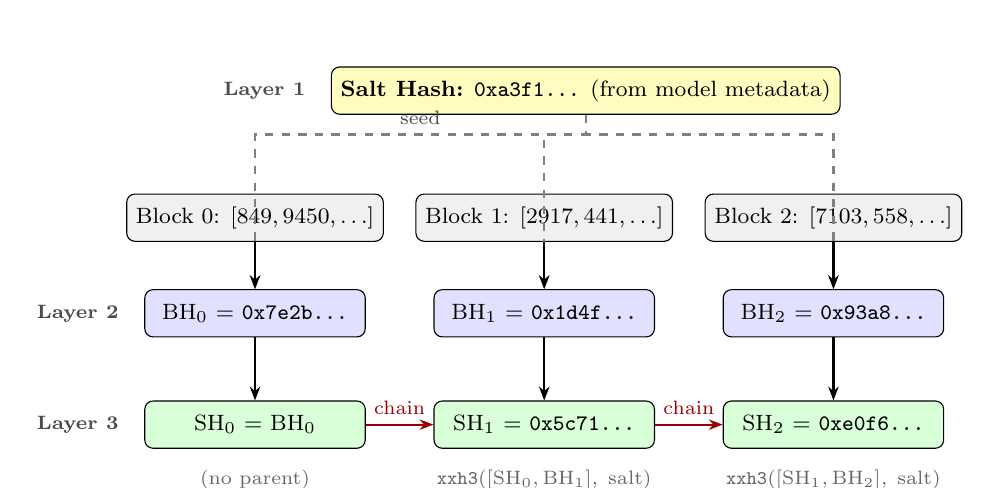
\begin{tikzpicture}[
    node distance=0.6cm,
    box/.style={draw, rounded corners=3pt, minimum height=0.7cm, font=\small},
    hashbox/.style={draw, rounded corners=3pt, minimum height=0.6cm, fill=blue!12, font=\footnotesize},
    seqbox/.style={draw, rounded corners=3pt, minimum height=0.6cm, fill=green!15, font=\footnotesize},
    saltbox/.style={draw, rounded corners=3pt, minimum height=0.6cm, fill=yellow!25, font=\footnotesize},
    tokenbox/.style={draw, rounded corners=3pt, minimum height=0.6cm, fill=gray!12, font=\footnotesize},
    arrow/.style={-{Stealth[length=5pt]}, thick},
    dasharrow/.style={-{Stealth[length=5pt]}, thick, dashed},
    lbl/.style={font=\scriptsize, text=black!70}
  ]

  % Layer 1: Salt
  \node[saltbox, minimum width=3.5cm] (salt) {\textbf{Salt Hash:} \texttt{0xa3f1...} (from model metadata)};
  \node[lbl, left=0.2cm of salt] {\textbf{Layer 1}};

  % Token blocks
  \node[tokenbox, below=1.0cm of salt, xshift=-4.2cm, minimum width=2.8cm] (t0) {Block 0: $[849, 9450, \ldots]$};
  \node[tokenbox, right=0.4cm of t0, minimum width=2.8cm] (t1) {Block 1: $[2917, 441, \ldots]$};
  \node[tokenbox, right=0.4cm of t1, minimum width=2.8cm] (t2) {Block 2: $[7103, 558, \ldots]$};

  % Layer 2: Block hashes
  \node[hashbox, below=0.6cm of t0, minimum width=2.8cm] (bh0) {BH\textsubscript{0} = \texttt{0x7e2b...}};
  \node[hashbox, below=0.6cm of t1, minimum width=2.8cm] (bh1) {BH\textsubscript{1} = \texttt{0x1d4f...}};
  \node[hashbox, below=0.6cm of t2, minimum width=2.8cm] (bh2) {BH\textsubscript{2} = \texttt{0x93a8...}};
  \node[lbl, left=0.2cm of bh0] {\textbf{Layer 2}};

  % Arrows: salt -> block hashes (seed)
  \draw[dasharrow, black!50] (salt.south) -- ++(0,-0.25) -| (bh0.north) node[pos=0.25, above, lbl] {seed};
  \draw[dasharrow, black!50] (salt.south) -- ++(0,-0.25) -| (bh1.north);
  \draw[dasharrow, black!50] (salt.south) -- ++(0,-0.25) -| (bh2.north);

  % Arrows: tokens -> block hashes (data)
  \draw[arrow] (t0) -- (bh0);
  \draw[arrow] (t1) -- (bh1);
  \draw[arrow] (t2) -- (bh2);

  % Layer 3: Sequence hashes
  \node[seqbox, below=0.8cm of bh0, minimum width=2.8cm] (sh0) {SH\textsubscript{0} = BH\textsubscript{0}};
  \node[seqbox, below=0.8cm of bh1, minimum width=2.8cm] (sh1) {SH\textsubscript{1} = \texttt{0x5c71...}};
  \node[seqbox, below=0.8cm of bh2, minimum width=2.8cm] (sh2) {SH\textsubscript{2} = \texttt{0xe0f6...}};
  \node[lbl, left=0.2cm of sh0] {\textbf{Layer 3}};

  % Arrows: block hash -> sequence hash
  \draw[arrow] (bh0) -- (sh0);
  \draw[arrow] (bh1) -- (sh1);
  \draw[arrow] (bh2) -- (sh2);

  % Arrows: chain (sequence hash of previous feeds into next)
  \draw[arrow, red!60!black] (sh0.east) -- (sh1.west) node[midway, above, lbl, text=red!60!black] {chain};
  \draw[arrow, red!60!black] (sh1.east) -- (sh2.west) node[midway, above, lbl, text=red!60!black] {chain};

  % Annotation: first block special case
  \node[lbl, below=0.15cm of sh0, text=black!60] {(no parent)};

  % Annotation: formula for SH_1
  \node[lbl, below=0.15cm of sh1, text=black!60, align=center] {$\texttt{xxh3}([\text{SH}_0, \text{BH}_1],\; \text{salt})$};

  % Annotation: formula for SH_2
  \node[lbl, below=0.15cm of sh2, text=black!60, align=center] {$\texttt{xxh3}([\text{SH}_1, \text{BH}_2],\; \text{salt})$};

\end{tikzpicture}
\caption{The three-layer hashing pipeline for a 3-block token sequence. Layer~1 (salt) derives a seed from model metadata. Layer~2 hashes each block's tokens independently using the salt as seed, producing content-addressable block hashes (BH). Layer~3 chains each block hash with its predecessor's sequence hash (SH), incorporating positional context. The first block's sequence hash equals its block hash; subsequent blocks fold in all prior history via the red chain arrows.}
\label{fig:hash-pipeline}
\end{figure}

\bigskip
With the three-layer scheme producing 64-bit sequence hashes, the next question is how to pack these hashes---along with position and content information---into a single lookup key for the radix tree.

\subsection{The 128-Bit Positional Sequence Hash}

\marginnote{\emph{Bit packing:} encoding multiple values into the sub-fields of a single integer, using bit shifts and masks to extract components. A common systems technique for reducing memory per entry.}%
The 64-bit sequence hash captures prefix history but does not explicitly encode the block's position or its content hash as separately queryable fields. For the radix tree, Dynamo needs all three in a single lookup key. The \texttt{PositionalSequenceHash} packs them into 128 bits using a variable-width encoding:

\begin{verbatim}
pub struct PositionalSequenceHash(u128);
// Layout of upper 64 bits:
//   [mode (2 bits)][position (P bits)][local_block_hash (R bits)]
// Lower 64 bits: SequenceHash
//
// Modes (auto-selected based on position):
//   Mode 00: 8-bit position + 54-bit LBH
//   Mode 01: 16-bit position + 46-bit LBH
//   Mode 10: 24-bit position + 38-bit LBH
//   Mode 11: 31-bit position + 31-bit LBH
\end{verbatim}

The mode is selected automatically based on the position value, using the smallest representation that fits. Most sequences have fewer than 256 blocks (mode 0), giving 54 bits for the local block hash---more than enough for near-zero collision probability at practical scale. For exceptionally long sequences (positions up to $2^{31} - 1$), mode 3 trades block hash precision for position range.

\begin{whynotbox}{Why a 128-bit packed hash instead of three separate fields?}
The radix tree (Chapter~\ref{ch:kvrouter}) uses a \texttt{DashMap<K, V>} keyed by block hash. Each lookup involves hashing the key, probing the table, and comparing keys for equality. If the key were a struct with three separate 64-bit fields (sequence hash, block hash, position), each lookup would hash $3 \times 8 = 24$ bytes and compare 24 bytes on each probe. The 128-bit packed representation halves both costs to 16 bytes.

More importantly, a struct-of-fields invites partial use: a programmer might accidentally compare only the sequence hash, forgetting that two blocks at the same position in different sequences could (with low probability) collide on sequence hash alone. By packing everything into a single opaque \texttt{u128}, the type makes partial comparison impossible---equality checks always consider all three components. The variable-width mode encoding is the price of this safety: it adds a few bit-shift operations per encode/decode, but these are trivially cheap compared to the hash table probe they accompany.
\end{whynotbox}

The encoding and decoding use straightforward bit manipulation:

\begin{verbatim}
fn encode_upper(mode: u8, position: u64,
                local_block_hash: u64) -> u64 {
    let (position_bits, lbh_bits) = match mode {
        0 => (8, 54), 1 => (16, 46),
        2 => (24, 38), 3 => (31, 31),
        _ => unreachable!(),
    };
    let position_mask = (1u64 << position_bits) - 1;
    let lbh_mask = (1u64 << lbh_bits) - 1;
    ((mode as u64) << 62)
        | ((position & position_mask) << lbh_bits)
        | (local_block_hash & lbh_mask)
}
\end{verbatim}

\subsection{Lineage Hashing for Tree Traversal}

The \texttt{PositionalSequenceHash} enables forward lookups---given a sequence, find which worker has its blocks cached. But the radix tree also needs \emph{backward traversal}: given a block at position $k$, find its parent at position $k - 1$. The \texttt{PositionalLineageHash} encodes both the current block's sequence hash fragment and the parent's:

\begin{verbatim}
pub struct PositionalLineageHash(u128);
// Layout: [mode (2)][position (P)][parent_frag (M)][current_frag (N)]
// Mode 00: 8-bit pos + 59-bit parent + 59-bit current
// Mode 01: 16-bit pos + 55-bit parent + 55-bit current
// Mode 10: 24-bit pos + 51-bit parent + 51-bit current
\end{verbatim}

A subtle correctness challenge arises at mode boundaries. When position 255 (mode 0, 59-bit fragments) is the parent of position 256 (mode 1, 55-bit fragments), the parent fragment stored at position 256 has only 55 bits, while the current fragment at position 255 has 59 bits. The constructor handles this with \emph{cross-mode alignment}: it computes the fragment width available at the \emph{next} position and truncates the current hash accordingly:

\begin{verbatim}
let next_mode = Self::select_mode(position + 1);
let (_, next_parent_bits, _) = Self::bit_layout(next_mode);
let aligned_current_bits = current_bits.min(next_parent_bits);
\end{verbatim}

This ensures that the current fragment at position $k$ always matches the parent fragment stored at position $k + 1$, even when the two positions use different encoding modes.

\begin{notebox}
The lineage hash limits positions to $2^{24} - 1$ (about 16.7 million blocks), stricter than the sequence hash's $2^{31} - 1$ limit. At a block size of 16, this supports sequences of up to 268 million tokens---well beyond current model context windows. The constructor panics if this limit is exceeded, a deliberate design choice rather than a silent truncation.
\end{notebox}

\bigskip
The hashing scheme gives each block a rich, position-aware identity. But hashes are only meaningful for \emph{complete} blocks---a half-filled block has no stable hash. How does Dynamo ensure that no code accidentally hashes a partial block, or mutates a block after its hash has been computed? The answer lies in Rust's type system.


\section{The Type-State Pattern}
\label{sec:tokens:typestate}

\marginnote{\emph{Type-state pattern:} using Rust's type system to encode an object's lifecycle state, making invalid state transitions a compile-time error rather than a runtime check.}%
Dynamo's token block system uses a carefully designed type hierarchy to enforce correct block lifecycle at compile time. While it does not use the classic generic-parameter type-state pattern (\texttt{Block<State>}), it achieves the same safety guarantees through distinct types for each lifecycle phase.

\subsection{Two Types, Two Phases}

A block in Dynamo exists in one of two states, represented by two entirely separate types:

\begin{enumerate}
  \item \textbf{\texttt{PartialTokenBlock}}: A block under construction. Tokens can be appended one at a time via \texttt{push\_tokens}. No hash has been computed. The block cannot be inserted into the radix tree or used for cache lookups.
  \item \textbf{\texttt{TokenBlock}}: A completed, immutable block. All $B$ tokens are present, the block hash, sequence hash, positional sequence hash, and positional lineage hash have all been computed. The block is ready for cache insertion and prefix matching.
\end{enumerate}

The transition between states is the \texttt{commit()} method, which \emph{consumes} the partial block's token data and produces a \texttt{TokenBlock}:

\begin{verbatim}
// PartialTokenBlock -> TokenBlock (via commit)
pub fn commit(&mut self) -> Result<TokenBlock, TokenBlockError> {
    if self.tokens.0.len() != self.block_size as usize {
        return Err(TokenBlockError::Incomplete);
    }
    let tokens = std::mem::take(&mut self.tokens);
    let chunk = TokenBlockChunk::new(tokens, self.salt_hash);
    let block = TokenBlock::from_chunk(
        chunk, self.parent_sequence_hash, self.position
    );
    // ... reset self for next block ...
    Ok(block)
}
\end{verbatim}

Several design choices enforce correctness:

\textbf{No \texttt{Clone} on \texttt{PartialTokenBlock}.}\hspace{1em} The \texttt{PartialTokenBlock} type deliberately omits \texttt{Clone} (the source code comments: ``No Clone: intended to be unique within a sequence''). This prevents accidentally duplicating a partial block and having two copies at different stages of completion, which would lead to hash chain corruption.

\textbf{Explicit error on incomplete commit.}\hspace{1em} Calling \texttt{commit()} on a block with fewer than $B$ tokens returns \texttt{Err(TokenBlockError::Incomplete)} rather than silently padding. This forces callers to handle the partial-block case explicitly.

\textbf{Immutability of \texttt{TokenBlock}.}\hspace{1em} Once created, a \texttt{TokenBlock} exposes only accessor methods (\texttt{tokens()}, \texttt{block\_hash()}, \texttt{sequence\_hash()}, etc.). There are no setters. The block's hashes are computed once in \texttt{from\_chunk} and can never be invalidated by mutation.

\subsection{The Intermediate: \texttt{TokenBlockChunk}}

Between \texttt{PartialTokenBlock} and \texttt{TokenBlock}, Dynamo introduces a private intermediate type:

\begin{verbatim}
struct TokenBlockChunk {
    tokens: Tokens,
    salt_hash: SaltHash,
    block_hash: BlockHash,
}
\end{verbatim}

A chunk has computed its block hash (Layer 2) but not yet its sequence hash (Layer 3), which depends on the parent block. This separation would enable parallel hash computation: all chunks in a batch can compute their block hashes independently, and only the sequential chaining step requires ordering. The \texttt{split\_tokens} function exploits this structure, computing all chunks in a batch before sequentially chaining them:

\begin{verbatim}
let chunks: Vec<TokenBlockChunk> = tokens
    .chunks_exact(block_size as usize)
    .map(|chunk| TokenBlockChunk::from_tokens(chunk, salt_hash))
    .collect();
// Sequential chaining:
for (position, chunk) in chunks.into_iter().enumerate() {
    let new_block = TokenBlock::from_chunk(
        chunk, last_sequence_hash, position
    );
    last_sequence_hash = Some(new_block.sequence_hash());
    result_blocks.push(new_block);
}
\end{verbatim}

\subsection{Partial Blocks in the UniqueBlock Enum}

For the broader system (beyond the tokens crate), blocks are identified via the \texttt{UniqueBlock} enum:

\begin{verbatim}
pub enum UniqueBlock {
    PartialBlock(Uuid),    // Identified by UUID (incomplete)
    FullBlock(GlobalHash), // Identified by hash (complete)
}
\end{verbatim}

Partial blocks cannot be content-addressed (their hash is not yet known), so they receive a random UUID. Full blocks are identified by their deterministic hash. This enum prevents the system from accidentally looking up a partial block by hash---the type makes the two identification schemes mutually exclusive.

\begin{insightbox}
The type-state pattern is a zero-cost abstraction: the state distinctions exist only at compile time and are erased during code generation. At runtime, the compiler generates the same machine code it would for a single \texttt{struct} with no state tracking. The safety guarantees---no hashing a partial block, no mutating a committed block, no cloning an in-progress block---come entirely from the compiler, with zero runtime overhead.
\end{insightbox}

\bigskip
The type system ensures that blocks are constructed correctly. But correctness at creation time is only half the story---blocks must also be managed correctly throughout their entire lifetime in the system, from arrival through sharing to eventual eviction.


\section{Memory Lifecycle}
\label{sec:tokens:lifecycle}

With the type system enforcing block correctness, we can now trace the full lifecycle of a token block through the system---from the moment a request arrives to the moment the block's memory is reclaimed.

\subsection{Phase 1: Arrival and Blocking}

When a request arrives, the frontend tokenizes the prompt and constructs a \texttt{TokenBlockSequence}:

\begin{verbatim}
let seq = TokenBlockSequence::new(tokens, block_size, Some(salt_hash));
\end{verbatim}

This immediately splits the tokens into complete \texttt{TokenBlock}s and a trailing \texttt{PartialTokenBlock}. Each complete block has its full hash chain computed. The sequence is now ready for routing.

\subsection{Phase 2: Routing via Hash Lookup}

The router (Chapter~\ref{ch:kvrouter}) takes the completed blocks' \texttt{PositionalSequenceHash} values and queries the \texttt{PositionalRadixTree}---a two-level \texttt{DashMap} indexed first by position, then by hash:

\begin{verbatim}
pub struct PositionalRadixTree<V, K = PositionalSequenceHash>
where K: PositionalHash + Hash + Eq + Clone,
{
    map: DashMap<u64, DashMap<K, V>>,
}
\end{verbatim}

The outer map partitions entries by block position. The inner map stores hash-to-value mappings for all blocks at that position. This two-level structure enables efficient prefix matching: the router iterates from position 0 upward, checking each block's hash against the tree, until it finds the longest matching prefix. The worker with the most cached blocks is selected.

\subsection{Phase 3: Prefill and Decode}

The selected worker receives the token sequence. During \emph{prefill}, the worker processes all prompt tokens through the transformer's attention layers, producing KV cache entries for each block. These entries are stored in GPU memory in block-sized slots---one slot per \texttt{TokenBlock}.

During \emph{decode} (autoregressive generation), each new token is appended to the sequence via \texttt{append()}:

\begin{verbatim}
pub fn append(&mut self, token: Token)
    -> Result<Option<usize>, TokenBlockError>
\end{verbatim}

If the new token completes a block (fills the partial block to $B$ tokens), the block is committed, its hashes are computed, and the method returns \texttt{Ok(Some(index))} with the index of the newly completed block. The system can then insert this block's hash into the radix tree, making it available for future requests to share.

\subsection{Phase 4: Sharing via Prefix Matching}

When a subsequent request arrives with a partially overlapping prefix, the router finds the matching blocks in the radix tree and routes the request to the worker that already has them cached. The new request skips prefill for the shared blocks and only processes the divergent suffix. This is the core mechanism of KV-cache-aware routing (Chapter~\ref{ch:kvrouter}).

The sharing is safe because blocks are immutable after commitment. Two requests can reference the same \texttt{TokenBlock} without any risk of one modifying the other's cached data.

\subsection{Phase 5: Mutation and Truncation}

Real serving workloads require sequence mutation. A speculative decoding system may need to retract tokens that were incorrectly predicted. The \texttt{TokenBlockSequence} supports this through \texttt{pop}, \texttt{truncate}, and \texttt{unwind}:

\begin{verbatim}
pub fn truncate(&mut self, len: usize)
    -> Result<(), TokenBlockError>
pub fn unwind(&mut self, count: usize)
    -> Result<(), TokenBlockError>
pub fn pop(&mut self) -> Option<Token>
\end{verbatim}

Truncation is more complex than appending. If the new length falls within the current partial block, only partial-block tokens are removed. If it crosses into committed blocks, entire \texttt{TokenBlock}s must be discarded and the partial block must be reconstructed from the surviving tokens of the first affected block.

\begin{bugbox}
The truncation logic contains a defensive \texttt{block\_size.max(1)} call to prevent division by zero if \texttt{block\_size} is somehow zero despite the constructor's assertion. This belt-and-suspenders approach reflects a real concern: the \texttt{block\_size} field is a plain \texttt{u32}, not a newtype that enforces non-zero, so a bug in deserialization or configuration could bypass the constructor's check. Our fuzzer exercised this path by constructing \texttt{TokenBlockSequence} values with block sizes from 1 to 16, confirming that the truncation arithmetic is correct for all non-zero sizes. The \texttt{div\_ceil(block\_size)} pattern with zero block sizes remains a recurring vulnerability across the codebase---we found it in \texttt{selector.rs}, \texttt{protocols.rs}, and \texttt{push\_router.rs}.
\end{bugbox}

\subsection{Phase 6: Eviction}

When GPU memory pressure requires reclamation, blocks are evicted. The eviction order is typically LRU (least recently used): blocks that have not been accessed by any recent request are evicted first. When a block is evicted, its hash is removed from the radix tree and its memory slot is returned to the free pool.

This heuristic works well for LLM serving because popular system prompts (``You are a helpful assistant...'') are accessed frequently and remain cached, while one-off conversational turns are evicted quickly. The result is that the most valuable cache entries---those shared by the largest number of requests---naturally survive the longest.

\begin{insightbox}
The memory lifecycle mirrors OS virtual memory management: allocation from a free pool, active use with sharing (analogous to copy-on-write pages), and eviction under pressure with an LRU policy. The key addition is the hash-based sharing mechanism: where an OS deduplicates identical pages reactively (e.g., KSM in Linux), Dynamo deduplicates proactively by hashing blocks at creation time and routing new requests to workers that already hold matching blocks.
\end{insightbox}


\section{Summary}

\begin{itemize}
  \item Token sequences are \textbf{partitioned into fixed-size blocks} of $B$ tokens, producing $\lceil n/B \rceil$ blocks per sequence. Partial trailing blocks are tracked separately and committed only when full.
  \item \textbf{Three-layer hashing} builds progressively richer identifiers: the \emph{salt hash} prevents cross-model collisions, the \emph{block hash} fingerprints content, and the \emph{sequence hash} chains blocks to incorporate positional context.
  \item The \textbf{128-bit positional sequence hash} packs sequence hash, block position, and local block hash into a single key using variable-width mode encoding, enabling efficient radix tree lookups.
  \item The \textbf{positional lineage hash} additionally encodes parent-child relationships, supporting backward traversal through the block chain with cross-mode boundary alignment.
  \item \textbf{Distinct types} for each lifecycle phase (\texttt{PartialTokenBlock}, \texttt{TokenBlockChunk}, \texttt{TokenBlock}, \texttt{UniqueBlock}) enforce correct state transitions at compile time with zero runtime cost.
  \item The \textbf{memory lifecycle} follows an arrive-block-route-prefill-share-evict progression, with LRU eviction naturally preserving high-value shared prefixes.
  \item Edge cases in block arithmetic (division by zero when $B = 0$, mode boundary alignment, partial-block truncation) are a recurring source of bugs found by fuzzing.
\end{itemize}

\bigskip
\begin{center}\rule{0.5\linewidth}{0.4pt}\end{center}
\bigskip

Blocks are now hashed, routed, and cached. But how does the data actually travel between services? The next chapter examines the binary wire format and the parsers that extract structured content from raw model output.

\bigskip
\noindent\textbf{Check Your Understanding}

\medskip
\noindent\emph{These questions are answerable from this chapter alone.}

\begin{enumerate}
  \item \textbf{Why must block hashing incorporate position, not just content?} Give a concrete example of incorrect behavior without positional hashing.

  \textit{Answer:} The KV cache entries for the same tokens differ depending on where those tokens appear in the sequence, because the transformer's positional encoding (RoPE, absolute, etc.) produces different attention patterns at different positions. Without positional hashing, the tokens ``Hello world'' at position 0 and the same tokens at position 8 would produce the same hash. The radix tree would incorrectly conclude they share a cache entry, causing the system to serve stale KV values computed with the wrong positional encoding---producing garbled output. The sequence hash chain prevents this: even with identical block hashes, different parent chains yield different sequence hashes.

  \item \textbf{Explain the three-layer hashing scheme.} What does each layer add, and why is it necessary?

  \textit{Answer:} Layer 1 (salt hash) hashes model metadata into a seed, preventing two different models from sharing cache entries for the same prompt. Layer 2 (block hash) hashes the $B$ token IDs within a block using the salt as seed, producing a content fingerprint. Layer 3 (sequence hash) chains each block hash with its parent's sequence hash, folding positional context into the identifier. Without the salt, cross-model pollution is possible. Without the block hash, the system cannot identify content-identical blocks. Without the sequence hash, position-dependent cache entries would be incorrectly shared.

  \item \textbf{What is the purpose of the variable-width mode encoding in \texttt{PositionalSequenceHash}?} Why not use a fixed layout?

  \textit{Answer:} The mode encoding allocates more bits to the local block hash when positions are small (mode 0: 54 bits for LBH) and trades LBH bits for position bits as positions grow (mode 3: 31 bits each). Since most sequences have fewer than 256 blocks, mode 0 applies to the vast majority of blocks, giving near-full 64-bit hash precision. A fixed 31-bit position field would waste 23 bits on every short-sequence block, reducing hash precision and increasing collision probability in the common case.

  \item \textbf{Why does \texttt{PartialTokenBlock} deliberately omit the \texttt{Clone} trait?}

  \textit{Answer:} A \texttt{PartialTokenBlock} represents a unique, in-progress accumulation point within a \texttt{TokenBlockSequence}. If it could be cloned, two copies could be filled independently, each computing different hashes when committed. The sequence hash chain requires a single linear progression---block $k$'s parent hash must be block $k-1$'s sequence hash. A cloned partial block would fork this chain, producing blocks with inconsistent ancestry. Omitting \texttt{Clone} makes this bug a compile-time error.

  \item \textbf{How does the lineage hash handle mode boundaries?} Why is cross-mode alignment necessary?

  \textit{Answer:} At position 255 (mode 0), the current hash fragment uses 59 bits. At position 256 (mode 1), the parent hash fragment uses only 55 bits. Without alignment, the parent fragment stored at position 256 would be a 55-bit truncation of a 59-bit value, and matching would fail. The constructor solves this by precomputing the next position's mode and truncating the current fragment to the minimum of the two widths: \texttt{aligned\_current\_bits = current\_bits.min(next\_parent\_bits)}. This ensures the current fragment at position $k$ is always a subset of the bits available for the parent fragment at position $k + 1$.

  \item \textbf{The chapter mentions that \texttt{block\_size = 0} causes panics across the codebase.} Why is this a realistic concern in a production system rather than a purely theoretical one?

  \textit{Answer:} Block size flows through multiple layers: configuration files, RPC messages, deserialization, and internal computation. A misconfigured YAML file, a zero-initialized protobuf field, or a default \texttt{u32} value (which is 0 in Rust) could propagate a zero block size past the constructor's assertion---especially in code paths that construct block-related values from deserialized network data rather than through the \texttt{TokenBlockSequence::new} constructor. Our fuzzer confirmed this by finding \texttt{div\_ceil(block\_size)} panics in three separate modules (\texttt{selector.rs}, \texttt{protocols.rs}, \texttt{push\_router.rs}), each receiving block size from a different source. Defense in depth---checking at every division site, not just the constructor---is the only reliable mitigation.
\end{enumerate}

\chapter{Network Codecs and Output Parsing}
\label{ch:codecs}

Every message exchanged between Dynamo's services---routing decisions, token sequences, model outputs, health checks---flows through a single binary codec. Every token generated by the model passes through a parser that extracts structured content (tool calls, reasoning traces, code blocks) from raw text. This chapter examines both: the \texttt{TwoPartCodec} that serializes inter-service communication, and the parser zoo that makes sense of model output. Together, they form Dynamo's data plane---the layer where bytes become meaning. Both are surprisingly rich sources of bugs: the codec's preamble handling contains an integer overflow that bypasses safety checks, and the parser zoo harbors panics, data corruption, and silent data loss across nearly every implementation.

%% ----------------------------------------------------------------
\section{The Wire Format}
\label{sec:codecs:wire}

\marginnote{\emph{Wire format:} the binary layout of data as it appears on the network, before deserialization.}%
Dynamo uses a custom binary protocol for all inter-service TCP communication. The protocol is designed for minimal overhead: no HTTP framing, no JSON parsing on the hot path, and no TLS within the trusted cluster (TLS terminates at the edge).

\begin{whynotbox}{{Why not use Protobuf, gRPC, or JSON?}}
The natural question is: why invent a custom binary protocol when mature alternatives exist? The answer is latency arithmetic. During autoregressive decoding, Dynamo generates one token every few milliseconds per request. Each token must travel from the GPU worker through the codec, across TCP, through the codec on the receiving end, and into the SSE stream to the user. At thousands of concurrent requests, the serialization layer processes millions of messages per second.

\textbf{JSON over HTTP} imposes per-field parsing overhead---field name lookups, string escaping, number parsing---that compounds at this scale. Even fast parsers like \texttt{simd-json} cannot avoid the fundamental cost of scanning for delimiters in a text format. HTTP framing adds further overhead: header parsing, chunked transfer encoding, and connection management.

\textbf{Protocol Buffers / gRPC} are binary and fast, but they impose schema management overhead: \texttt{.proto} files must be kept in sync between sender and receiver, the code generator must run at build time, and the generated code adds compilation cost. gRPC additionally requires HTTP/2 framing, which is overkill for a trusted internal cluster where TLS terminates at the edge.

Dynamo's wire format is simpler than either: a fixed-size 24-byte preamble followed by raw bytes. The receiver reads three integers and immediately knows how many bytes to consume---no parsing, no schema lookup, no framing negotiation. The trade-off is that the format is not self-describing: a version mismatch between sender and receiver causes silent corruption rather than a clean error. For an internal cluster where all services are deployed together, this trade-off is worthwhile.
\end{whynotbox}

Each message consists of three parts:

\begin{enumerate}
  \item \textbf{Preamble} (24 bytes, fixed): three \texttt{u64} fields---the header length, the body length, and an xxHash checksum.
  \item \textbf{Header} (variable length): metadata serialized with MessagePack (a compact binary JSON alternative). Contains routing information, request IDs, and codec version.
  \item \textbf{Body} (variable length): the payload---token sequences, model outputs, or control messages---serialized in a format determined by the message type.
\end{enumerate}

\begin{figure}[h]
\centering
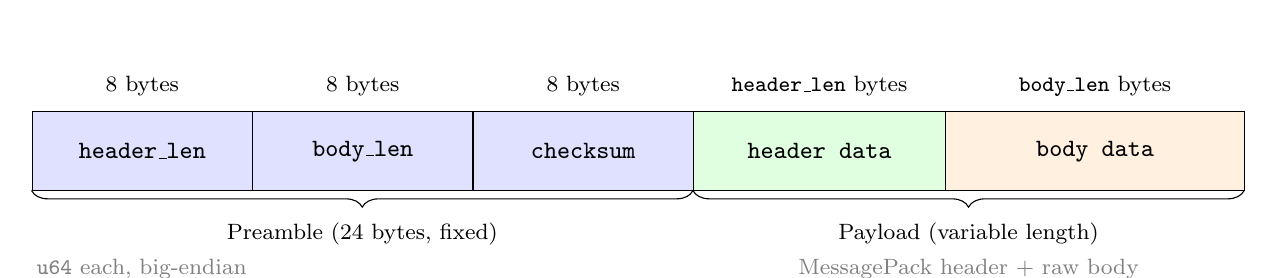
\begin{tikzpicture}[
    field/.style={draw, minimum height=1.0cm, font=\small\ttfamily, anchor=west},
    brace/.style={decorate, decoration={brace, amplitude=6pt, mirror}},
    label/.style={font=\footnotesize},
  ]
  % Preamble fields
  \node[field, fill=blue!12, minimum width=2.8cm] (hlen) at (0,0) {header\_len};
  \node[field, fill=blue!12, minimum width=2.8cm] (blen) at (2.8,0) {body\_len};
  \node[field, fill=blue!12, minimum width=2.8cm] (csum) at (5.6,0) {checksum};

  % Variable-length fields
  \node[field, fill=green!12, minimum width=3.2cm] (header) at (8.4,0) {header data};
  \node[field, fill=orange!12, minimum width=3.8cm] (body) at (11.6,0) {body data};

  % Byte-size labels above
  \node[label, above=2pt of hlen] {8 bytes};
  \node[label, above=2pt of blen] {8 bytes};
  \node[label, above=2pt of csum] {8 bytes};
  \node[label, above=2pt of header] {\texttt{header\_len} bytes};
  \node[label, above=2pt of body] {\texttt{body\_len} bytes};

  % Braces underneath
  \draw[brace] (0,-0.5) -- node[below=8pt, label] {Preamble (24 bytes, fixed)} (8.4,-0.5);
  \draw[brace] (8.4,-0.5) -- node[below=8pt, label] {Payload (variable length)} (15.4,-0.5);

  % Type annotations below braces
  \node[label, text=gray] at (1.4,-1.5) {\texttt{u64} each, big-endian};
  \node[label, text=gray] at (11.9,-1.5) {MessagePack header + raw body};
\end{tikzpicture}
\caption{The \texttt{TwoPartCodec} wire format. The fixed 24-byte preamble contains three \texttt{u64} fields that allow the receiver to determine the exact message size before reading the payload. The checksum is computed only in debug builds; release builds write zero for speed.}
\label{fig:twopart-wire}
\end{figure}

The fixed-size preamble allows the receiver to determine exactly how many bytes to read before parsing begins, enabling zero-allocation reads for small messages that fit in a pre-allocated buffer. This is a length-prefixed framing strategy, common in network protocols from MySQL's packet format to Redis's RESP3. The key advantage over delimiter-based framing (e.g., HTTP's \texttt{\textbackslash r\textbackslash n\textbackslash r\textbackslash n} header terminator) is that the receiver never needs to scan the payload for special characters---it reads exactly the number of bytes declared in the preamble, which means binary payloads require no escaping.

\begin{notebox}
The 24-byte preamble is the first thing the codec reads from the TCP stream. If the preamble is malformed---for example, if the header or body length fields contain values that would overflow when added---the codec must reject the message before allocating memory. This is exactly where Bug~\#3 (Chapter~\ref{ch:findings}) resides: the addition of header length and body length can overflow in release builds, silently bypassing the size check.
\end{notebox}

The wire format is intentionally \emph{not} self-describing: unlike JSON or Protocol Buffers, there are no field names or type tags in the preamble. The header and body are opaque byte sequences whose interpretation depends on the application layer. This keeps the codec layer thin and fast, but it means that a version mismatch between sender and receiver can cause silent data corruption rather than a clean error. Dynamo mitigates this by including a codec version in the MessagePack-encoded header, allowing the receiver to reject messages from incompatible versions.

Dynamo also defines a separate \texttt{TcpRequestMessage} wire format for the request plane, with a more structured layout:

\begin{verbatim}
  endpoint_path_len : u16    (2 bytes)
  endpoint_path     : UTF-8  (variable)
  headers_len       : u16    (2 bytes)
  headers           : JSON   (variable)
  payload_len       : u32    (4 bytes)
  payload           : bytes  (variable)
\end{verbatim}

This format carries routing metadata (the endpoint path) and trace headers inline, enabling the receiving service to dispatch the request without deserializing the payload. The payload itself uses zero-copy slicing via \texttt{bytes::Bytes::slice()}, so the router can forward it to a worker without touching the contents.

The two wire formats serve different roles in Dynamo's architecture. The \texttt{TwoPartCodec} format is used on the \emph{response plane}---the path that carries generated tokens from GPU workers back through the system. Its minimal 24-byte preamble reflects the performance sensitivity of this path: every token generated by every concurrent request passes through this codec. The \texttt{TcpRequestMessage} format is used on the \emph{request plane}---the path that carries user prompts to GPU workers. Requests are less frequent (one per user interaction rather than one per token), so the richer metadata format is affordable.

%% ----------------------------------------------------------------
\section{The TwoPartCodec}
\label{sec:codecs:twopart}

\marginnote{\emph{Tokio codec:} Tokio's \texttt{Decoder}/\texttt{Encoder} traits transform byte streams into typed message streams.}%
With the wire format established, we can now examine the code that reads and writes it. The \texttt{TwoPartCodec} implements Tokio's \texttt{Decoder} and \texttt{Encoder} traits, integrating with Rust's async I/O ecosystem. The core data structure is \texttt{TwoPartMessage}: a pair of \texttt{Bytes} values (header and body) that can be independently empty.

\begin{verbatim}
pub struct TwoPartMessage {
    pub header: Bytes,
    pub data: Bytes,
}
\end{verbatim}

The decoder operates as a state machine with two phases:

\textbf{Phase 1: Read preamble.} The codec checks whether at least 24 bytes are available in the read buffer. If not, it returns \texttt{Ok(None)}, telling Tokio to wait for more data. If 24 bytes are present, it reads three \texttt{u64} values using the \texttt{Buf} trait's \texttt{get\_u64()} method:

\begin{verbatim}
let header_len = cursor.get_u64() as usize;
let body_len   = cursor.get_u64() as usize;
let _checksum  = cursor.get_u64();

let total_len = 24 + header_len + body_len;
\end{verbatim}

\textbf{Phase 2: Read payload.} Using the lengths from the preamble, the codec checks whether \texttt{total\_len} bytes are available. If so, it advances past the 24-byte preamble, then calls \texttt{split\_to()} twice to extract the header and body as separate \texttt{Bytes} values:

\begin{verbatim}
let header = src.split_to(header_len).freeze();
let data   = src.split_to(body_len).freeze();
\end{verbatim}

The \texttt{split\_to()} + \texttt{freeze()} combination is the key to zero-copy operation: it splits the buffer at the given index without copying, then converts the mutable \texttt{BytesMut} slice into an immutable \texttt{Bytes} reference. The critical detail is that \texttt{split\_to(n)} operates in $O(1)$ time---it adjusts internal pointers rather than moving data. The underlying memory is shared between the original buffer and the split-off piece via reference counting.

\marginnote{\emph{xxHash:} a non-cryptographic hash function optimized for speed, producing 64-bit hashes at $\sim$30\,GB/s on modern CPUs.}%
The choice of xxHash-64 (\texttt{xxh3\_64} from the \texttt{xxhash-rust} crate) for the checksum is deliberate: it is one of the fastest non-cryptographic hash functions available, processing data at memory bandwidth on modern CPUs. Since the checksum is only computed in debug builds, its purpose is catching bugs during development, not protecting against adversarial corruption---TCP's own 16-bit checksum handles the latter (imperfectly, but adequately for a trusted cluster network).

The encoder reverses this process: given a \texttt{TwoPartMessage}, it writes the three \texttt{u64} preamble fields followed by the header and body bytes. Checksum computation is conditional: in debug builds, it computes an xxHash-64 over the concatenation of header and body; in release builds, it writes a zero checksum for speed, relying on TCP's own checksumming for integrity.

The \texttt{TwoPartMessage} type also provides convenience constructors for common patterns: \texttt{from\_header()} for control messages with no body, \texttt{from\_data()} for payloads with no routing header, and \texttt{into\_message\_type()} which classifies the message into one of four variants (\texttt{HeaderOnly}, \texttt{DataOnly}, \texttt{HeaderAndData}, \texttt{Empty}) for pattern matching in downstream handlers.

\begin{notebox}
The codec supports multiple messages concatenated in a single TCP buffer. Tokio's \texttt{FramedRead} adapter calls \texttt{decode()} in a loop until it returns \texttt{Ok(None)}, naturally handling message pipelining. This is important for performance: TCP's Nagle algorithm may coalesce multiple small messages into a single network packet, and the codec must correctly split them apart.
\end{notebox}

\begin{bugbox}
\textbf{Bug \#3: Integer overflow in preamble handling.} The codec reads \texttt{header\_len} and \texttt{body\_len} as \texttt{u64} values from the network, then computes \texttt{let total\_len = 24 + header\_len + body\_len}. All three operands are \texttt{usize} (64-bit on modern systems), but the addition can still overflow. Consider \texttt{header\_len = u64::MAX} and \texttt{body\_len = 1}: their sum wraps to zero, so \texttt{total\_len} becomes 24. If \texttt{max\_message\_size} is set to, say, 16\,MB, the check \texttt{total\_len > max\_size} passes (24 < 16\,MB), and the codec proceeds to read from the buffer using the original, enormous \texttt{header\_len}---causing an out-of-bounds read or an allocation of $2^{64} - 1$ bytes.

In Rust's debug build, the addition panics (denial of service). In release builds, the addition wraps silently via two's complement, potentially allowing an attacker-controlled payload to bypass length validation entirely. The fix is to use \texttt{checked\_add()}, which returns \texttt{None} on overflow:

\begin{verbatim}
let total_len = 24_usize
    .checked_add(header_len)
    .and_then(|n| n.checked_add(body_len))
    .ok_or(TwoPartCodecError::InvalidMessage(
        "Length overflow".to_string(),
    ))?;
\end{verbatim}

Note that the debug-mode checksum verification path \emph{does} use \texttt{checked\_add}---the developers were aware of the overflow risk in that code path but missed the earlier, more critical one in the main decode logic. This is a common pattern in security bugs: the fix is applied in one place but not another.
\end{bugbox}

%% ----------------------------------------------------------------
\section{Zero-Copy Decoding}
\label{sec:codecs:zerocopy}

\marginnote{\emph{Zero-copy:} processing data without copying it to a new memory location, operating directly on the original buffer.}%
The previous section described \emph{what} the codec reads; this section explains \emph{how} it avoids the most expensive part of reading: copying data. For high-throughput message processing, copying data between buffers is a significant cost. A single \texttt{memcpy} of a 4\,KB token sequence takes roughly 200 nanoseconds---trivial in isolation, but at one million messages per second, that is 200 milliseconds of CPU time per second consumed purely by copying. The codec is designed to eliminate this cost.

The mechanism is Rust's \texttt{bytes} crate, which provides two core types:

\begin{itemize}
  \item \texttt{BytesMut}: a mutable, growable byte buffer with reference-counted backing storage. Tokio's framed reader fills this buffer with data from the TCP socket.
  \item \texttt{Bytes}: an immutable, cheaply cloneable view into a \texttt{BytesMut} buffer. Cloning a \texttt{Bytes} value increments a reference count---it does not copy the underlying data.
\end{itemize}

The \texttt{Buf} and \texttt{BufMut} traits provide cursor-like access to these buffers. \texttt{Buf::get\_u64()} reads 8 bytes and advances the cursor; \texttt{BufMut::put\_u64()} writes 8 bytes and advances. These traits allow the codec to read and write structured fields without manual index arithmetic.

The zero-copy flow works as follows:

\begin{enumerate}
  \item Tokio reads TCP data into a \texttt{BytesMut} buffer (a single allocation, reused across messages).
  \item The codec's \texttt{decode()} method calls \texttt{src.split\_to(header\_len)}, which cleaves the buffer at the given offset. The original buffer retains bytes after the split point; the returned \texttt{BytesMut} owns the bytes before it. No data is copied.
  \item The codec calls \texttt{.freeze()} on the split result, converting \texttt{BytesMut} to \texttt{Bytes}. This makes the buffer immutable and enables cheap cloning.
  \item The resulting \texttt{Bytes} header and body are passed to the deserialization layer, which can further \texttt{.slice()} them without copying.
\end{enumerate}

The trade-off is that zero-copy decoding holds a reference to the original buffer's backing allocation, preventing it from being reused until all slices are dropped. For long-lived messages (e.g., streaming responses that persist for the duration of generation), this can increase peak memory usage. For the response plane, Dynamo also provides a \texttt{ZeroCopyTcpDecoder} that uses the same \texttt{split\_to/freeze} pattern for the request message format, extracting the payload as \texttt{Bytes::slice()} directly from the read buffer.

The response-plane codec (\texttt{TcpResponseCodec}) uses an even simpler format: a 4-byte \texttt{u32} length prefix followed by the data bytes. This minimalism reflects the asymmetry of inference serving: requests carry rich metadata (endpoint paths, trace headers, routing information), while responses are often just serialized token sequences that need minimal framing. The response codec's \texttt{decode()} method follows the same two-phase pattern as \texttt{TwoPartCodec}: peek at the length, check availability, then \texttt{split\_to().freeze()}.

\begin{notebox}
The \texttt{TcpRequestMessage} format uses \texttt{u16} for endpoint path and header lengths, limiting each to 65\,535 bytes, and \texttt{u32} for payload length, limiting payloads to 4\,GB. These limits are enforced both in encoding (reject oversized inputs before writing) and decoding (reject malformed length fields before allocating). This belt-and-suspenders approach prevents both memory exhaustion from malicious inputs and silent truncation from overflow.
\end{notebox}

\begin{insightbox}
The zero-copy pattern explains why Dynamo uses \texttt{Bytes} pervasively rather than \texttt{Vec<u8>}. A \texttt{Vec<u8>} must be cloned with a full copy; a \texttt{Bytes} is cloned with an atomic reference count increment (a single CPU instruction on x86). When a single incoming message is fanned out to multiple downstream consumers---as happens during broadcast or multi-worker routing---the difference is substantial.
\end{insightbox}

%% ----------------------------------------------------------------
\section{TCP Connection Management}
\label{sec:codecs:tcp}

\marginnote{\emph{Framed adapter:} Tokio's \texttt{Framed\-Read}/\texttt{Framed\-Write} wrappers apply a codec to a raw byte stream, producing a typed \texttt{Stream} of messages.}%
The codec knows how to encode and decode individual messages, but it does not manage the connections those messages flow over. That is the responsibility of the TCP connection layer. Dynamo maintains persistent TCP connections between services, using connection pooling to amortize the cost of TCP handshakes. Each connection is wrapped in a Tokio \texttt{Framed} adapter that applies the \texttt{TwoPartCodec} to the raw byte stream, producing a stream of typed \texttt{TwoPartMessage} values.

The server side (\texttt{TcpStreamServer}) binds to a port using the \texttt{socket2} crate for fine-grained control over socket options (e.g., \texttt{SO\_REUSEADDR}). When a client connects, the server splits the TCP stream into read and write halves, wraps each in a \texttt{FramedRead} or \texttt{FramedWrite} with the appropriate codec, and hands them to the pipeline.

Connection establishment uses a ``call home'' handshake: the worker connects to the router (rather than the router connecting to the worker), sends a \texttt{CallHomeHandshake} identifying itself, and the router registers the connection. This design simplifies firewall rules in containerized deployments---workers initiate outbound connections, which is generally permitted by default.

Connection health is monitored through heartbeat messages: the router periodically sends a ping, and the worker must respond within a timeout. If a worker fails to respond, the router marks it as unhealthy and stops routing requests to it, then notifies the service discovery layer (etcd) to trigger a replacement.

Backpressure is handled at the connection level: if a worker's incoming message queue is full, the TCP flow control mechanism (window size) naturally slows the sender. The codec does not implement application-level backpressure beyond what TCP provides, relying on the OS network stack to regulate flow.

\begin{insightbox}
The ``call home'' design inverts the usual client-server relationship: the worker is the TCP client even though it is the service provider. This is a pragmatic choice for Kubernetes deployments where workers are ephemeral pods with dynamic IP addresses. Rather than requiring the router to discover worker addresses (via DNS, service mesh, or etcd polling), the worker connects to the router's well-known address at startup. The handshake message carries the worker's capabilities (GPU type, available memory, supported models), allowing the router to begin routing immediately.
\end{insightbox}

The Tokio \texttt{FramedRead} and \texttt{FramedWrite} adapters deserve special mention. They bridge the gap between Tokio's byte-oriented \texttt{AsyncRead}/\texttt{AsyncWrite} traits and the message-oriented \texttt{Stream}/\texttt{Sink} traits. The \texttt{FramedRead} adapter maintains an internal \texttt{BytesMut} buffer, reads bytes from the socket into it, then repeatedly calls the codec's \texttt{decode()} method until it returns \texttt{Ok(None)} (not enough data) or an error. This loop handles the case where a single TCP read delivers multiple complete messages---common under high load when the OS batches socket reads.

%% ----------------------------------------------------------------
\section{The Parser Zoo}
\label{sec:codecs:parsers}

\marginnote{\emph{Parser zoo:} Dynamo's collection of 17+ model-specific output parsers, each handling a different model family's output format.}%
The codec and TCP layers handle \emph{transport}: getting bytes reliably from one service to another. But once a message arrives, a second challenge begins: making sense of the \emph{content}. For model output in particular, this is where things get messy.

Large language models do not produce structured output. They produce raw text---a stream of tokens decoded back into characters. But applications need structure: tool call invocations with JSON arguments, reasoning traces separated from final answers, code blocks with language annotations. The \emph{parser zoo} is Dynamo's collection of model-specific parsers that extract this structure from raw text.

Why are there so many parsers? Because there is no standard tool-call format. The OpenAI API defines a \emph{response} format for tool calls (a JSON object with \texttt{name} and \texttt{arguments} fields), but it does not standardize the \emph{output} format---the raw text that the model generates before it is parsed into that response structure. Each model family invented its own convention for how the model should emit tool calls in its token stream:

\begin{itemize}
  \item \textbf{Hermes/Llama3/Mistral/Phi4}: JSON-based formats with start/end delimiter tokens (e.g., \texttt{<TOOLCALL>...\allowbreak</TOOLCALL>}).
  \item \textbf{DeepSeek V3}: custom delimiters with Unicode special characters: \texttt{<|tool\_call\_begin|>}.
  \item \textbf{DeepSeek V3.1/V3.2 (DSML)}: ``DeepSeek Markup Language,'' a full XML-like format with Unicode delimiters and typed parameters.
  \item \textbf{GLM-4.7} (Zhipu AI): XML with nested tags such as \texttt{<tool\_call>}, \texttt{<arg\_key>}, and \texttt{<arg\_value>}.
  \item \textbf{Kimi K2} (Moonshot AI): section-delimited format with \texttt{<|tool\_call\_begin|>} tokens and \texttt{functions.name:index} identifiers.
  \item \textbf{XML/Qwen3 Coder}: generic XML with \texttt{<function=name>\allowbreak <parameter=key>value\allowbreak </parameter>\allowbreak </function>}.
  \item \textbf{Pythonic}: Python function call syntax---\texttt{[get\_weather(city="SF")]}.
  \item \textbf{Harmony}: an async JSON-based format requiring concurrent processing.
  \item \textbf{MiniMax M2}: yet another JSON variant with model-specific quirks.
\end{itemize}

This diversity is the price of a decentralized ecosystem: without a single authority mandating a wire format, each model trainer chose whatever format their training data and chat templates made convenient. The serving infrastructure must handle them all.

\begin{whynotbox}{Why so many parser implementations instead of one unified parser?}
Given the bug density of the parser zoo (the majority of bugs cataloged in Chapter~\ref{ch:findings} reside in parsers), a natural design question is: why not define a single, well-tested parser that all models funnel through?

The answer is that the formats are \emph{genuinely different}, not superficial variations. Hermes uses JSON between XML-like delimiters. DeepSeek DSML uses a full XML-like markup with typed attributes. GLM-4.7 uses key-value tag pairs. The Pythonic format is literal Python syntax. You cannot write a single regex or grammar that handles all of these---the syntactic structures are incompatible. A ``unified parser'' would need to be a full parser combinator framework with pluggable grammars, which is effectively what the current enum-dispatched architecture already is, just with hand-written parsers instead of generated ones.

The deeper problem is that model trainers control the output format, not the serving infrastructure. A model is trained to emit tool calls in a specific syntax baked into its training data and chat template. Changing the format would require retraining the model. The serving layer has no choice but to meet each model where it is.

What \emph{could} be unified---and would reduce bugs---is the streaming state machine logic. Every parser faces the same streaming challenge (detecting partial delimiters, buffering across token boundaries, handling boundary mismatches), and each reimplements it independently. A shared streaming harness with pluggable delimiter sets would eliminate an entire class of bugs.
\end{whynotbox}

The parser architecture unifies these behind two trait interfaces:

\textbf{Tool call parsing} uses a dispatcher pattern. A static \texttt{PARSER\_MAP} (initialized via \texttt{OnceLock}) maps parser names to \texttt{ToolCallConfig} structs. Each config specifies the parser variant via a \texttt{ParserConfig} enum:

\begin{verbatim}
pub enum ParserConfig {
    Json(JsonParserConfig),
    Pythonic,
    Xml(XmlParserConfig),
    Dsml(DsmlParserConfig),
    Glm47(Glm47ParserConfig),
    KimiK2(KimiK2ParserConfig),
    Harmony(JsonParserConfig),
    Typescript,  // Not yet implemented
}
\end{verbatim}

The entry point, \texttt{try\_tool\_call\_parse()}, dispatches on this enum to the appropriate parser implementation. Each parser returns a \texttt{(Vec<ToolCallResponse>, Option<String>)} tuple: the parsed tool calls and any remaining normal text. A \texttt{ToolCallResponse} contains three fields: a unique ID, a type (currently always \texttt{Function}), and a \texttt{CalledFunction} with the function name and JSON-serialized arguments:

\begin{verbatim}
pub struct ToolCallResponse {
    pub id: String,
    pub tp: ToolCallType,
    pub function: CalledFunction,
}
pub struct CalledFunction {
    pub name: String,
    pub arguments: String,  // JSON
}
\end{verbatim}

\textbf{Reasoning parsing} uses a trait-object pattern. The \texttt{ReasoningParser} trait defines two methods:

\begin{verbatim}
pub trait ReasoningParser: Send + Debug {
    fn detect_and_parse_reasoning(
        &mut self, text: &str, token_ids: &[u32]
    ) -> ParserResult;

    fn parse_reasoning_streaming_incremental(
        &mut self, text: &str, token_ids: &[u32]
    ) -> ParserResult;
}
\end{verbatim}

The first method handles one-shot (complete) inputs; the second handles streaming, returning only the \emph{delta} (newly discovered text) for each chunk. The \texttt{ParserResult} struct splits text into \texttt{reasoning\_text} and \texttt{normal\_text}. Implementations include \texttt{BasicReasoningParser} (handles \texttt{<think>...</think>} with configurable delimiters, used by DeepSeek R1, Qwen3, Kimi K2.5, and Mistral), \texttt{GraniteReasoningParser} (natural-language delimiters like ``Here's my thought process:''), \texttt{GptOssReasoningParser} (GPT-compatible reasoning extraction), and \texttt{MiniMaxAppendThinkParser}. The diversity of delimiter styles is remarkable: DeepSeek uses XML tags, Kimi (original) uses Unicode triangular brackets (\texttt{<<think>>}), Mistral uses bracketed tags (\texttt{[THINK]...[/THINK]}), and Granite uses natural English sentences.

The \texttt{ReasoningParser} trait is wrapped in a \texttt{ReasoningParserWrapper} that holds a \texttt{Box<dyn ReasoningParser>}, enabling dynamic dispatch. A factory method \texttt{get\_reasoning\_parser\_from\_name()} looks up the parser type by string name from a global \texttt{OnceLock}-backed map and returns the appropriate wrapper. Unknown names fall back to the basic \texttt{<think>...</think>} parser with a warning---a resilient default that prevents misconfiguration from crashing the system.

\begin{notebox}
The parser zoo currently maps 17 named parsers to 9 distinct implementations. Several models share implementations: Nemotron Nano reuses Qwen3 Coder's parser, GLM-4.5 reuses the basic \texttt{<think>} parser. The \texttt{OnceLock}-based global map means these mappings are established once and cached for the process lifetime---which becomes a source of bugs when the mapping depends on runtime configuration (see Bug~\#11, the Kimi K2 \texttt{OnceLock} caching issue).
\end{notebox}

%% ----------------------------------------------------------------
\section{Tool Call Parsing}
\label{sec:codecs:toolcalls}

\marginnote{\emph{Tool call:} a structured invocation embedded in model output, specifying a function name and JSON arguments.}%
Tool calls are the primary structured output that parsers must extract. When a model is prompted with a list of available tools, it may respond with a tool invocation---a function name and arguments---embedded in its text output. This section walks through how the major parsers handle this, and where they break.

Each parser implements three functions that mirror the lifecycle of a streaming tool call:

\begin{enumerate}
  \item \texttt{detect\_tool\_call\_start(chunk)} --- returns \texttt{true} if the chunk contains (or ends with a prefix of) the tool call start token. This is used by the streaming layer to switch from ``emit text'' mode to ``buffer tool call'' mode.
  \item \texttt{find\_tool\_call\_end\_position(chunk)} --- returns the byte offset after the end token, or the chunk length if the end token has not yet appeared. This tells the streaming layer how much of the buffered text constitutes a complete tool call that can be handed to the parser.
  \item \texttt{try\_tool\_call\_parse(message)} --- the main parsing function, called once a complete tool call block has been accumulated. Returns structured tool calls and any non-tool-call text that was adjacent to the tool call block.
\end{enumerate}

The partial-prefix detection in step 1 deserves attention. Consider a streaming scenario where the model outputs the text ``Some text <tool\_c'' in one chunk. The start token \texttt{<tool\_call>} is not fully present, but the chunk \emph{ends with a prefix of it}. The parser must recognize this partial match and begin buffering, because the next chunk might complete the token. All parsers use a shared utility function \texttt{chunk\_ends\_with\_token\_prefix()} for this check, which iterates over successively longer suffixes of the chunk to see if any is a prefix of the start token. This function was itself a source of bugs before being fixed: the original byte-based implementation panicked on multi-byte UTF-8 start tokens (e.g., the Chinese CJK characters meaning ``tool'' characters used in some GLM configurations).

\subsection{The XML Parser Family}

The XML parser handles formats like Qwen3 Coder, where tool calls look like:

\begin{verbatim}
<tool_call>
<function=get_weather>
<parameter=city>San Francisco</parameter>
<parameter=unit>fahrenheit</parameter>
</function>
</tool_call>
\end{verbatim}

The parser uses regex to extract function blocks and parameter blocks from within each \texttt{<tool\_call>...</tool\_call>} region. Parameters are typed using the tool's JSON Schema: if the schema says \texttt{city} is a string and \texttt{count} is an integer, the parser coerces accordingly. Without a schema, all values are returned as strings. The type coercion logic is extensive, recognizing aliases like \texttt{int}/\texttt{integer}/\texttt{int32}/\texttt{int64}, \texttt{float}/\texttt{number}/\texttt{double}, \texttt{boolean}/\texttt{bool}/\texttt{binary}, \texttt{object}/\texttt{dict}/\texttt{dictionary}, and \texttt{array}/\texttt{arr}/\texttt{list}.

The parser is also deliberately fault-tolerant with missing closing tags. If \texttt{</parameter>} is absent, the regex's non-greedy match extends to the next \texttt{<parameter=} or \texttt{</function>} tag, capturing the value with trailing markup. If both \texttt{</parameter>} and \texttt{</function>} are missing, the value extends to the \texttt{</tool\_call>} tag---including the closing tag itself in the value. This matches the behavior of the upstream SGLang Python implementation, trading correctness for resilience against malformed model output.

The XML parser contains two bugs found by fuzzing:

\begin{bugbox}
\textbf{Bug \#13: \texttt{strip\_quotes} panics on single-character input.} The utility function \texttt{strip\_quotes()} removes surrounding quotes from a string. It checks \texttt{starts\_with('"') \&\& ends\_with('"')}, then returns \texttt{\&trimmed[1..trimmed.len()-1]}. But when the input is a single quote character \texttt{"}, both conditions are true (a single-char string both starts and ends with that character), and the slice becomes \texttt{[1..0]}---an invalid range. Rust panics with ``begin <= end'' violated. This is a classic off-by-one: the code assumes quoted strings are at least two characters long.
\end{bugbox}

\begin{bugbox}
\textbf{Bug \#12: \texttt{try\_literal\_eval} corrupts string values.} The XML parser falls back to a Python \texttt{ast.literal\_eval}-style parser for non-JSON values. This function performs global string replacements: \texttt{.replace("True", "true")}, \texttt{.replace("False", "false")}, \texttt{.replace("None", "null")}. These replacements are not context-aware---they corrupt substrings within quoted values. The input \texttt{\{'location': 'TrueNorth'\}} becomes \texttt{\{"location": "trueNorth"\}}, silently corrupting the string ``TrueNorth'' to ``trueNorth''. Similarly, ``Falsehood'' becomes ``falsehood'' and ``NoneAvailable'' becomes ``nullAvailable''.
\end{bugbox}

\subsection{The GLM-4.7 Parser}

GLM-4.7 (Zhipu AI) uses a distinct XML dialect where arguments are structured as key-value tag pairs rather than attributes:

\begin{verbatim}
<tool_call>get_weather
  <arg_key>location</arg_key>
  <arg_value>San Francisco</arg_value>
</tool_call>
\end{verbatim}

The parser extracts the function name as everything between \texttt{<tool\_call>} and the first \texttt{<arg\_key>}, then uses a regex to match \texttt{<arg\_key>...</arg\_key><arg\_value>...</arg\_value>} pairs. Values are coerced using the tool's schema (integers, booleans, arrays, etc.), with XML entity decoding (\texttt{\&lt;} $\rightarrow$ \texttt{<}) applied before parsing. The parser also handles multi-line argument values, which is essential for code-generation tool calls.

\begin{bugbox}
\textbf{Bug \#1: UTF-8 boundary panic in GLM-4.7 parser.} The parser extracts the function name by trimming whitespace from the content between \texttt{<tool\_call>} and the first \texttt{<arg\_key>}. It then computes the arguments section as \texttt{content[function\_name.len()..]}\,---using the \emph{trimmed} name's byte length as an offset into the \emph{untrimmed} content. When there is leading whitespace and the function name contains multi-byte UTF-8 characters (e.g., CJK characters like CJK characters meaning ``get weather''), the byte offset lands in the middle of a UTF-8 code point, and Rust panics with ``byte index is not a char boundary.'' For ASCII function names with leading whitespace, the offset is merely wrong (off by the whitespace length), but the regex still finds arguments---silently producing correct results by accident. With multi-byte characters, the bug becomes a crash.
\end{bugbox}

\subsection{The Pythonic Parser}

The Pythonic parser handles models (e.g., Jamba, some Llama variants) that emit tool calls as Python expressions:

\begin{verbatim}
[get_weather(city="San Francisco"), set_alarm(time="8:00")]
\end{verbatim}

Rather than writing a custom parser, Dynamo uses the \texttt{rustpython-parser} crate to parse this as a Python AST. The expression is parsed in \texttt{Mode::Expression}, and the AST is walked to extract function names and keyword arguments. This is elegant---it handles nested data structures (lists, dicts) and Python literals (booleans, None) natively. The AST walker recursively converts Python constants to JSON values: \texttt{True} $\rightarrow$ \texttt{true}, \texttt{None} $\rightarrow$ \texttt{null}, Python integers to JSON numbers (with fallback to strings for values outside the \texttt{i64}/\texttt{u64} range), and Python dicts and lists to their JSON equivalents.

A pre-processing regex identifies candidate tool call blocks in the input. The pattern matches the outer \texttt{[...]} list containing one or more \texttt{func(key=val)} calls. The regex is compiled once via \texttt{OnceLock} and reused across invocations. Text before the first match is returned as ``normal text''; the matched block is passed to the Python parser.

However, the approach has bugs:

\begin{bugbox}
\textbf{Bug \#7: Pythonic parser prefix leak and text loss.} The parser has multiple issues. First, it extracts ``normal text'' as \texttt{stripped.split(\&matches[0]).next()}---which returns only text \emph{before} the first match. Any text after the tool call is silently dropped. Second, adjacent identifier characters are absorbed into the function name, corrupting the extracted name. Third, the regex pattern requires at least one \texttt{key=value} argument, so a zero-argument call like \texttt{[get\_time()]} is treated as normal text rather than a tool call.
\end{bugbox}

\subsection{The JSON Parser Family}

The JSON-based parsers handle the largest number of model families: Hermes, Llama 3, Mistral, Phi4, Nemotron, Jamba, MiniMax M2, and the DeepSeek V3/V3.1 variants. The common pattern is: find text between configurable start and end delimiter tokens, then parse the enclosed content as JSON. The JSON object is expected to contain a function name key and an arguments key:

\begin{verbatim}
<TOOLCALL>{"name": "get_weather",
           "arguments": {"city": "SF"}}</TOOLCALL>
\end{verbatim}

DeepSeek V3 uses a more complex format with Unicode delimiters and a type/separator structure:

\begin{verbatim}
<|tool_call_begin|>function<|tool_sep|>get_weather
```json
{"city": "SF"}
```<|tool_call_end|>
\end{verbatim}

The JSON parser extracts blocks using regex, then calls \texttt{serde\_json::from\_str} to parse each block. DeepSeek V3.1 adds a further complication: it uses both ``individual call'' delimiters (\texttt{tool\_call\_begin/end}) and ``wrapper'' delimiters (\texttt{tool\_calls\_begin/end}) that enclose multiple calls. The parser must filter delimiter tokens to find the right level of nesting. The \texttt{JsonParserConfig} is accordingly flexible, with separate fields for start tokens, end tokens, separator tokens, function name keys, and argument keys---all as \texttt{Vec<String>} to accommodate models that use different keys (e.g., \texttt{"name"} vs.\ \texttt{"function"}, \texttt{"arguments"} vs.\ \texttt{"parameters"}).

Note that DeepSeek V3's coverage from generic fuzz targets was zero---the Unicode delimiter tokens are unlikely to appear in random input. Achieving meaningful coverage required constructing parser-specific fuzz targets with structured inputs that include the correct delimiter tokens, a challenge we discuss further in Chapter~\ref{ch:fuzzing}.

\subsection{The DSML Parser}

DeepSeek V3.2 introduced DSML (DeepSeek Markup Language), a full XML-like format with Unicode-heavy delimiters:

\begin{verbatim}
<|DSML|function_calls>
<|DSML|invoke name="get_weather">
<|DSML|parameter name="city" string="true">
  San Francisco
</|DSML|parameter>
</|DSML|invoke>
</|DSML|function_calls>
\end{verbatim}

Each parameter carries a \texttt{string="true|false"} attribute indicating whether the value should be treated as a literal string or parsed as JSON. The parser uses regex to extract invoke blocks and parameter blocks, then conditionally parses values based on this flag. The DSML format is notable for its use of fullwidth Unicode pipe characters (\texttt{|}, U+FF5C) in its delimiters---these serve as visual markers that are extremely unlikely to appear in natural text, reducing false-positive detection. The downside is that these characters are multi-byte in UTF-8 (3 bytes each), making byte-level string manipulation error-prone.

\begin{bugbox}
\textbf{Bug \#10: DSML parser silently drops parameters.} The regex that matches \texttt{<|DSML|parameter name="..."} requires the \texttt{string} attribute to be present. If the model omits the \texttt{string} attribute (which happens for non-string parameters in some model configurations), the regex does not match, and the parameter is silently dropped from the parsed output. The tool call succeeds but with missing arguments---a silent data loss bug.
\end{bugbox}

\subsection{The Kimi K2 Parser}

Kimi K2 (Moonshot AI) uses section delimiters and a \texttt{functions.name:index} naming convention:

\begin{verbatim}
<|tool_calls_section_begin|>
<|tool_call_begin|>
functions.get_weather:0
<|tool_call_argument_begin|>
{"city": "SF"}
<|tool_call_end|>
<|tool_calls_section_end|>
\end{verbatim}

The function ID is parsed with a secondary regex that strips the optional \texttt{functions.} prefix and extracts the name and index components. The arguments are expected to be a JSON object between the \texttt{argument\_begin} and \texttt{call\_end} tokens.

The parser compiles its main regex from the config tokens using \texttt{OnceLock}, caching it for the process lifetime. The pattern captures two named groups: \texttt{function\_id} (matching the \texttt{[\textbackslash w.]+:\textbackslash d+} format) and \texttt{arguments} (the JSON object). This leads to:

\begin{bugbox}
\textbf{Bug \#11: \texttt{OnceLock} caches stale regex.} The Kimi K2 parser stores its compiled regex in a \texttt{static OnceLock<Regex>}. The regex pattern is built from the \texttt{KimiK2ParserConfig}'s delimiter tokens. But \texttt{OnceLock::get\_or\_init} only runs the initialization closure once---the first time it is called. If the process handles requests for multiple Kimi K2 model variants with different delimiter configurations (e.g., singular \texttt{tool\_call\_section\_begin} vs.\ plural \texttt{tool\_calls\_section\_begin}), the regex cached from the first variant is silently used for all subsequent variants. Tool calls from the second variant fail to match.
\end{bugbox}

\subsection{The Granite Reasoning Parser}

\marginnote{\emph{Streaming mismatch:} when one-shot and streaming parsing produce different results for the same input.}%
The Granite parser (IBM's model family) separates reasoning from content using natural-language delimiters: ``Here's my thought process:'' and ``Here's my response:''. The parser accepts multiple variants of each delimiter (e.g., ``Here's my thought process:'' and ``Here is my thought process:'') to handle the model's non-deterministic phrasing. Unlike XML tags, these delimiters can appear as substrings of normal text, making boundary detection fragile. The parser maintains internal state (\texttt{in\_reasoning}, \texttt{stripped\_think\_start}, a text buffer) to track its position in the reasoning/content split across streaming chunks.

\begin{bugbox}
\textbf{Bug \#8: Granite streaming mismatches.} The one-shot parser (\texttt{detect\_and\_parse\_reasoning}) and the streaming parser (\texttt{parse\_reasoning\_streaming\_incremental}) produce different results for the same input. The one-shot parser uses \texttt{.find()} to locate delimiters in the complete text; the streaming parser accumulates text in a buffer and checks for delimiters at each token boundary. When a delimiter spans a token boundary (e.g., ``Here's my '' in one token and ``thought process:'' in the next), the streaming parser may detect it at a different point than the one-shot parser, causing the split between reasoning and content to differ.
\end{bugbox}

The MiniMax Append Think parser exhibits a similar class of streaming mismatch (Bug~\#9): its one-shot and streaming modes disagree on where reasoning text ends and normal text begins, particularly when the \texttt{<think>} block is empty or contains only whitespace.

\begin{insightbox}
The streaming parsing problem is fundamentally harder than batch parsing. In batch mode, the parser sees the entire input and can use global context to locate boundaries. In streaming mode, it sees one token at a time and must decide---before the next token arrives---whether the current token is inside a tool call, outside one, or at a boundary. A single misclassified token can cause the parser to lose synchronization: buffering text that is not a tool call (causing latency), or emitting raw text that was meant to be a structured argument (causing data corruption). Every streaming parser bug we found involves these boundary transitions. This is not a coincidence: streaming parsers are state machines operating on partial information, and state machines are precisely the class of program where fuzzers excel at finding unexpected state transitions.
\end{insightbox}

%% ----------------------------------------------------------------
\section{Summary}
\label{sec:codecs:summary}

\begin{itemize}
  \item The \textbf{wire format} uses a 24-byte fixed preamble (header length, body length, checksum) followed by variable-length header and body payloads. A separate request-plane format adds endpoint routing and trace headers.
  \item The \textbf{TwoPartCodec} implements Tokio's codec traits for async encoding and decoding, with a two-phase state machine (preamble, then payload). The checksum is only computed in debug builds; release builds write zero for performance.
  \item \textbf{Zero-copy decoding} via \texttt{BytesMut::split\_to().freeze()} avoids allocation on the hot path, using reference-counted byte slices that can be cheaply cloned and sliced without copying data.
  \item \textbf{TCP connection management} uses persistent pooled connections with a call-home handshake and heartbeat-based health monitoring. Backpressure relies on TCP flow control.
  \item The \textbf{parser zoo} contains 17 named parsers mapping to 9 distinct implementations behind enum-dispatched and trait-object interfaces. The proliferation is driven by the absence of a standard tool-call format across model families.
  \item \textbf{Tool call parsing} is a streaming problem where boundary misclassification leads to data loss or corruption---the dominant bug category found by fuzzing. Of the 16 bugs cataloged in Chapter~\ref{ch:findings}, the majority reside in parsers.
\end{itemize}

Table~\ref{tab:parser-bugs} summarizes the parser bugs discussed in this chapter, organized by severity.

\medskip
\begin{table}[h]
\centering
\small
\begin{tabular}{llll}
\hline
\textbf{Bug} & \textbf{Parser} & \textbf{Category} & \textbf{Severity} \\
\hline
\#1  & GLM-4.7           & UTF-8 boundary panic       & Crash \\
\#13 & XML strip\_quotes  & Slice range panic          & Crash \\
\#3  & TwoPartCodec      & Integer overflow           & Critical \\
\#8  & Granite           & Streaming mismatch         & Correctness \\
\#9  & MiniMax           & Streaming mismatch         & Correctness \\
\#11 & Kimi K2           & OnceLock stale cache       & Logic \\
\#10 & DSML              & Silent parameter drop      & Logic \\
\#7  & Pythonic          & Prefix leak                & Logic \\
\#12 & XML literal\_eval  & String value corruption    & Correctness \\
\hline
\end{tabular}
\caption{Parser and codec bugs found by fuzzing, discussed in this chapter.}
\label{tab:parser-bugs}
\end{table}

\medskip
\begin{center}\rule{0.5\linewidth}{0.4pt}\end{center}
\medskip

The codec and parser layers occupy opposite ends of the complexity spectrum: the codec is a single, well-specified state machine with one critical bug; the parser zoo is a sprawling collection of ad-hoc text processors with bugs in nearly every implementation. Both are essential to Dynamo's operation, and both benefit enormously from fuzzing.

We have now mapped every component of Dynamo's architecture, from the transformer inside the GPU through the distributed system that orchestrates a fleet. The next two chapters shift from understanding the system to breaking it: Chapter~\ref{ch:fuzzing} introduces the fuzzing methodology, and Chapter~\ref{ch:findings} catalogs what we found.

\medskip
\noindent\textbf{Check Your Understanding}

\smallskip
\noindent\emph{These questions are answerable from this chapter alone.}

\begin{enumerate}
  \item Why does Dynamo use a custom binary protocol rather than HTTP/JSON or Protocol Buffers for inter-service communication? What latency characteristics make this choice necessary?

  \emph{Answer: During autoregressive decoding, Dynamo generates millions of messages per second (one token per request per step, at thousands of concurrent requests). JSON parsing imposes per-field overhead; Protocol Buffers require schema management and code generation. Dynamo's length-prefixed binary format allows the receiver to determine message boundaries from a fixed 24-byte preamble without parsing any content, enabling zero-allocation reads and zero-copy buffer sharing via the \texttt{bytes} crate.}

  \item Explain how the TwoPartCodec's two-phase design (preamble then payload) enables efficient reading from a TCP stream.

  \emph{Answer: In phase 1, the codec reads exactly 24 bytes to learn the header and body lengths. If fewer than 24 bytes are available, it returns \texttt{Ok(None)} and Tokio waits for more data. In phase 2, it reads exactly \texttt{header\_len + body\_len} bytes. This two-phase approach means the codec never reads more data than needed, never speculatively parses partial messages, and can pre-allocate the exact buffer size---avoiding both over-allocation and reallocation.}

  \item What is the integer overflow vulnerability in the codec's preamble handling? Why does it manifest differently in debug vs.\ release builds?

  \emph{Answer: The computation \texttt{24 + header\_len + body\_len} can overflow when \texttt{header\_len} and \texttt{body\_len} are attacker-controlled \texttt{u64} values cast to \texttt{usize}. In debug builds, Rust's default arithmetic panics on overflow, causing a denial-of-service crash. In release builds, Rust uses wrapping (two's complement) arithmetic by default, so the overflow produces a small \texttt{total\_len} that passes the \texttt{max\_message\_size} check, allowing the attacker to bypass length validation.}

  \item Why is tool call parsing particularly prone to bugs? What makes the streaming (token-by-token) constraint harder than batch parsing?

  \emph{Answer: In batch mode, the parser sees the complete input and can use global search to find delimiters. In streaming mode, it must classify each token as it arrives---inside a tool call, outside, or at a boundary---without future context. Delimiters that span token boundaries may be detected at different points than in batch mode. A single misclassified token causes synchronization loss: the parser either buffers normal text (increasing latency) or emits tool call content as raw text (causing data corruption).}

  \item The \texttt{try\_literal\_eval} function in the XML parser performs \texttt{.replace("True", "true")}. Why is this problematic, and what is a correct alternative?

  \emph{Answer: The replacement is global and not context-aware---it corrupts substrings within quoted string values (e.g., ``TrueNorth'' becomes ``trueNorth''). A correct implementation would only replace Python keywords that appear as standalone tokens outside of string literals. This could be done by first tokenizing the input to identify string boundaries, then only replacing bare keywords, or by using a proper Python literal parser.}

  \item How does the GLM-4.7 parser's function name extraction lead to a UTF-8 boundary panic? What is the root cause?

  \emph{Answer: The parser extracts the function name by trimming whitespace from the content between \texttt{<tool\_call>} and \texttt{<arg\_key>}. It then uses the trimmed name's byte length as an offset into the untrimmed content: \texttt{content[function\_name.len()..]}. When there is leading whitespace and the function name contains multi-byte UTF-8 characters, the byte offset is wrong (off by the whitespace bytes), and may land in the middle of a multi-byte code point. Rust's string slicing requires char-aligned boundaries and panics otherwise.}

  \item Explain the \texttt{OnceLock} caching bug in the Kimi K2 parser. Under what deployment scenario does it cause failures?

  \emph{Answer: The parser stores its compiled regex in a \texttt{static OnceLock}, which initializes exactly once per process. The regex pattern is built from the parser's configuration tokens. If a single process serves multiple Kimi K2 model variants with different delimiter configurations, the regex cached from the first variant is used for all subsequent variants. Tool calls from variants with different delimiters fail to match the cached regex, causing silent tool call detection failures.}

  \item Why does the Pythonic parser use the \texttt{rustpython-parser} crate to parse tool calls, and what are its limitations?

  \emph{Answer: The Pythonic format (\texttt{[func(key=val)]}) is valid Python syntax, so using a real Python parser avoids reimplementing Python's expression grammar---it correctly handles nested lists, dicts, keyword arguments, and Python literals (True, False, None) natively. The limitations are: (1) the regex that detects tool calls requires at least one argument, rejecting zero-argument calls like \texttt{[get\_time()]}; (2) the normal-text extraction uses \texttt{split().next()}, which only captures text before the first match, silently dropping text after the tool call.}
\end{enumerate}

\chapter{Fuzzing the System}
\label{ch:fuzzing}

The previous chapters explained how Dynamo works. This chapter explains how we broke it. \emph{Fuzzing} is an automated testing technique that generates random or semi-random inputs and feeds them to a program, looking for crashes, hangs, or incorrect behavior. When applied systematically to Dynamo's Rust libraries, it found 16 bugs across 36 fuzz targets in approximately 141 million test executions. This chapter explains what fuzzing is, how coverage-guided fuzzing works, why the oracle problem is the central challenge, and how we designed and executed the campaign.


\section{What Is Fuzzing?}
\label{sec:fuzzing:what}

\marginnote{\emph{Fuzzing:} automated testing by generating inputs and observing whether the program crashes or misbehaves.}%
At its simplest, fuzzing is feeding garbage to a program and seeing what happens. The insight that makes it powerful is that programs often fail on inputs their developers never considered---not because the developers were careless, but because the space of possible inputs is astronomically large. A function that processes a byte sequence has $256^n$ possible inputs of length $n$. No amount of hand-written unit tests can cover more than a vanishingly small fraction of this space.

Fuzzing automates the search through this space. A \emph{fuzzer} generates inputs, feeds them to the target function (called the \emph{harness}), observes the result, and repeats---millions or billions of times. The simplest fuzzers generate completely random bytes. More sophisticated fuzzers use feedback from the program's execution to guide their search toward interesting inputs.

\subsection{A Brief History}

The idea is older than most programmers realize. In 1988, Barton Miller at the University of Wisconsin assigned his graduate students a simple project: write a program that generates random characters and pipes them to Unix utilities. A startling number of standard tools---including programs in \texttt{/usr/bin} that had been in production for years---crashed or hung. The lesson was immediate: software that works on expected inputs often fails spectacularly on unexpected ones.

\marginnote{\emph{AFL:} American Fuzzy Lop, a landmark coverage-guided fuzzer released by Michal Zalewski in 2013.}%
For two decades, fuzzing remained a niche technique. The breakthrough came with \emph{coverage-guided fuzzing}, pioneered by tools like AFL (American Fuzzy Lop, 2013) and LLVM's libFuzzer. These tools use code coverage as a feedback signal: if a mutated input reaches new code paths, the fuzzer saves it and mutates it further. This transforms fuzzing from random bombardment into an evolutionary search through the program's state space. Google's OSS-Fuzz project, launched in 2016, runs continuous fuzzing on hundreds of open-source projects and has found over 10,000 bugs.

In the Rust ecosystem, the standard tool is \texttt{cargo-fuzz}, which wraps libFuzzer with Rust-specific support for structured input generation via the \texttt{Arbitrary} trait. This is what we used for the Dynamo campaign.

\begin{notebox}
Fuzzing Rust code differs from fuzzing C/C++ in a fundamental way. In C, the primary targets are memory corruption bugs: buffer overflows, use-after-free, and null dereferences. In safe Rust, these bugs are eliminated by the compiler. The bugs that remain---and that our fuzzer found---are panics (denial of service), logic errors (silent data corruption), and debug/release divergence (different behavior depending on build profile). This shifts the fuzzer's role from ``find memory safety violations'' to ``find crashes and semantic bugs.''
\end{notebox}

\begin{whynotbox}{Why not use property-based testing instead of fuzzing?}
Property-based testing (PBT) frameworks like QuickCheck and proptest also generate random inputs and check assertions. The key difference is \emph{feedback}. PBT generates inputs from a distribution defined by the programmer---it has no visibility into which code paths a given input exercises. Coverage-guided fuzzing uses runtime instrumentation to \emph{observe} which branches each input takes, then preferentially mutates inputs that reach new code. This means fuzzing can discover deep, multi-step code paths that PBT's distribution would almost never produce. PBT is better when you have strong domain knowledge about the input distribution and want to verify specific properties. Fuzzing is better when you want to explore the full input space, including edge cases you did not anticipate. In practice, the two techniques are complementary: we used \texttt{Arbitrary} (a PBT-style input generator) \emph{inside} the coverage-guided fuzzing loop, getting the best of both.
\end{whynotbox}


\section{Coverage-Guided Fuzzing}
\label{sec:fuzzing:coverage}

\marginnote{\emph{Coverage-guided fuzzing:} using code coverage feedback to guide input generation toward unexplored execution paths.}%
Pure random fuzzing is inefficient: most random inputs exercise the same few code paths (early validation checks, error returns). \emph{Coverage-guided fuzzing} solves this by instrumenting the target program to report which code paths each input exercises. When an input reaches a new code path (a branch not previously taken, a function not previously called), the fuzzer saves it as a \emph{seed} and mutates it to explore further.

The feedback loop works as follows:
\begin{enumerate}
  \item The fuzzer generates or mutates an input.
  \item The harness runs with the input. Compiler instrumentation records which basic blocks and edges between them are executed.
  \item If the input triggered new coverage (reached code not previously reached by any input), the fuzzer adds it to its \emph{corpus}---a growing collection of interesting inputs.
  \item The fuzzer selects an input from the corpus, applies random mutations (bit flips, byte insertions, splicing two inputs together), and repeats from step 1.
\end{enumerate}

Over time, the corpus evolves toward inputs that collectively cover more of the target's code. The fuzzer automatically discovers edge cases, boundary values, and unusual code paths---not because it understands the code, but because the coverage feedback rewards inputs that explore new territory.

Figure~\ref{fig:fuzzing-loop} illustrates the feedback loop as a cycle. The key property is that the corpus grows monotonically: once an input discovers new coverage, it is never discarded (though it may be replaced during corpus minimization by a smaller input that covers the same edges).

\begin{figure}[ht]
\centering
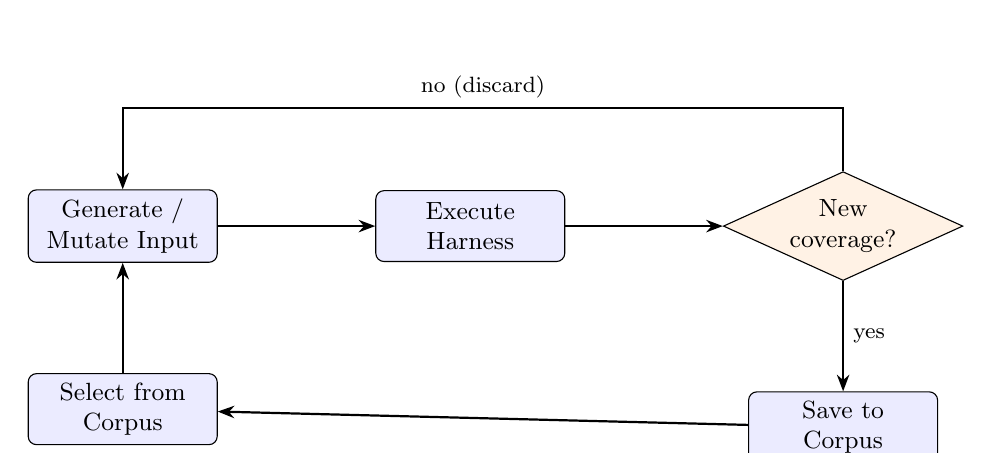
\begin{tikzpicture}[
    node distance=1.6cm,
    every node/.style={font=\small},
    block/.style={rectangle, draw, rounded corners=3pt, minimum width=2.4cm, minimum height=0.9cm, align=center, fill=blue!8},
    decision/.style={diamond, draw, aspect=2.2, inner sep=1pt, align=center, fill=orange!10},
    arr/.style={-{Stealth[length=6pt]}, thick},
]
    \node[block] (gen) {Generate /\\Mutate Input};
    \node[block, right=2.0cm of gen] (exec) {Execute\\Harness};
    \node[decision, right=2.0cm of exec] (cov) {New\\coverage?};
    \node[block, below=1.4cm of cov] (save) {Save to\\Corpus};
    \node[block, below=1.4cm of gen] (select) {Select from\\Corpus};

    \draw[arr] (gen) -- (exec);
    \draw[arr] (exec) -- (cov);
    \draw[arr] (cov) -- node[right, font=\footnotesize] {yes} (save);
    \draw[arr] (cov.north) -- ++(0,0.8) -| node[pos=0.25, above, font=\footnotesize] {no (discard)} (gen.north);
    \draw[arr] (save) -- (select);
    \draw[arr] (select) -- (gen);
\end{tikzpicture}
\caption{The coverage-guided fuzzing feedback loop. Inputs that discover new code paths are saved to the corpus; inputs that do not are discarded. The corpus grows monotonically, and mutations are drawn from it, creating an evolutionary search through the program's input space.}
\label{fig:fuzzing-loop}
\end{figure}

\subsection{How libFuzzer Works}

LibFuzzer, the engine behind \texttt{cargo-fuzz}, instruments the target binary at compile time using LLVM's SanitizerCoverage pass. This inserts a callback at every \emph{edge} in the control-flow graph---every branch between basic blocks. At runtime, libFuzzer maintains a coverage map: a fixed-size array where each entry corresponds to a hashed edge identifier. When an input exercises a previously unseen edge (or hits an edge a new number of times), it is ``interesting'' and is added to the corpus.

\marginnote{\emph{Corpus minimization:} reducing the corpus to the smallest set of inputs that preserves total coverage.}%
LibFuzzer also performs \emph{corpus minimization}: periodically removing inputs that are redundant (their coverage is a subset of other inputs' coverage). This keeps the corpus small and focused, which speeds up subsequent mutations. When a crash is found, libFuzzer performs \emph{crash minimization}: iteratively shrinking the crashing input while preserving the crash, producing a minimal reproducer.

\begin{insightbox}
Coverage-guided fuzzing is a form of evolutionary search. Inputs that explore new code paths are ``fit'' and survive (are kept in the corpus and mutated further). Inputs that cover only already-explored paths are ``unfit'' and discarded. The corpus gradually evolves toward comprehensive code coverage, with mutations acting as the variation mechanism and coverage feedback as the selection pressure.
\end{insightbox}

A concrete example from our campaign illustrates the power of this approach. The \texttt{fuzz\_codec\_\allowbreak crash\_oracle} target feeds random bytes to the \texttt{TwoPartCodec} decoder. Early random inputs all fail the length check (the decoder requires at least 24 bytes for the fixed preamble). But eventually, the fuzzer generates a 24-byte input that passes the length check and reaches the field-parsing code. This input is saved. Further mutations explore the space of valid-length inputs, eventually producing one where the \texttt{header\_len} and \texttt{body\_len} fields are near \texttt{u64::MAX}. The addition \texttt{24 + header\_len + body\_len} overflows, and the fuzzer records a crash.

No human tester would write a unit test with \texttt{header\_len = 0xFFFFFFFFFFFFFFFF}. The fuzzer discovered it because coverage feedback rewarded inputs that passed the length check, and random mutation eventually produced extreme field values. This is the core value proposition of coverage-guided fuzzing: it systematically explores the space of inputs that reach deep code paths, including corner cases that humans overlook.


\section{The Oracle Problem}
\label{sec:fuzzing:oracle}

\marginnote{\emph{Oracle:} a mechanism that determines whether a program's output is correct for a given input.}%
Fuzzing finds \emph{inputs}. But an input is only useful if we can determine whether the program's behavior on that input is correct or incorrect. This determination requires an \emph{oracle}---a source of truth about what the correct behavior should be. The \textbf{oracle problem} is the central challenge of fuzzing: crashes are easy to detect (the program aborts), but \emph{silent correctness bugs} are hard to detect because the program runs to completion and produces output that \emph{looks} fine.

We used four oracle strategies in the Dynamo campaign:

\textbf{Crash oracle.} The simplest: if the program panics, it is a bug. This catches division by zero, out-of-bounds indexing, \texttt{unwrap()} on \texttt{None}, integer overflow (in debug builds), and \texttt{RefCell} borrow violations. Every crash bug in Chapter~\ref{ch:findings} was found this way. The \texttt{fuzz\_codec\_crash\_oracle} target (Section~\ref{sec:fuzzing:infra}) is a pure crash oracle---it exercises five different decoders and asserts nothing, relying entirely on panics to signal bugs:

\begin{lstlisting}[language=Rust,caption={Crash oracle: the harness asserts nothing; any panic is a bug.}]
fuzz_target!(|data: &[u8]| {
    let bytes = Bytes::copy_from_slice(data);
    let codec = TwoPartCodec::new(None);
    let _ = codec.decode_message(bytes.clone());
    let codec_limited = TwoPartCodec::new(Some(1024));
    let _ = codec_limited.decode_message(bytes.clone());
    let _ = TcpRequestMessage::decode(&bytes);
    let _ = Frame::decode(bytes);
});
\end{lstlisting}

\textbf{Differential oracle.} Run two implementations on the same input and compare outputs. If they disagree, at least one has a bug. We used this for parsers (streaming vs.\ oneshot) and for the three KV-cache indexer implementations. Section~\ref{sec:fuzzing:differential} covers this in detail.

\textbf{Property oracle.} Assert invariants that must hold regardless of input. For example: the codec's round-trip property (encode then decode must return the original data), the radix tree's score bound (no score can exceed the query length), or the token block sequence's length tracking (total tokens must match the count of appends minus pops). These are embedded as \texttt{assert!} statements in the harness.

\textbf{Assertion oracle.} Embed postcondition checks that convert semantic expectations into crash signals. If a postcondition is violated, the assertion panics, and the fuzzer records it as a crash. For example, after \texttt{select\_worker} returns, we assert that the selected worker ID actually exists in the worker set:

\begin{lstlisting}[language=Rust,caption={Assertion oracle: postcondition check on worker selection.}]
match selector.select_worker(&workers, &request, block_size) {
    Ok(selection) => {
        assert!(workers.contains_key(&selection.worker.worker_id),
            "Selected worker {} not in worker set",
            selection.worker.worker_id);
    }
    Err(_) => {} // NoEndpoints is fine
}
\end{lstlisting}

\begin{notebox}
The oracle problem explains why 4 of the 16 bugs were found by code audit rather than fuzzing. Logic bugs like ``parser drops text after the second tool call'' produce output that differs from the correct result, but the fuzzer has no way to know what the correct result is unless we encode the expectation as a property or differential test. The code auditor, reading the specification and the code side by side, can spot the discrepancy directly.
\end{notebox}


\section{Structuring Inputs with Arbitrary}
\label{sec:fuzzing:arbitrary}

\marginnote{\emph{Arbitrary:} a Rust trait for generating structured values from raw bytes, bridging the gap between random byte streams and typed program inputs.}%
Most of Dynamo's functions do not accept raw byte slices. The router expects a list of token IDs and a worker configuration. The parser expects a model output string and a tool specification. The codec expects a preamble with specific field widths. Feeding random bytes to these functions would waste most of the fuzzer's effort on inputs rejected by early validation.

The \texttt{Arbitrary} trait (from the \texttt{arbitrary} crate) solves this by defining how to construct structured values from raw bytes. By deriving \texttt{Arbitrary} on the input types, we let the fuzzer generate valid-by-construction inputs: token ID sequences of realistic lengths, configuration structs with plausible field values, and model output strings containing the delimiters that parsers look for.

\subsection{Before: Manual Byte Parsing}

Without \texttt{Arbitrary}, the harness author must manually decode the fuzzer's byte stream into structured parameters. This is tedious and error-prone. Here is how the \texttt{fuzz\_worker\_selector} target parses configuration from raw bytes:

\begin{lstlisting}[language=Rust,caption={Manual input parsing: extracting structured fields from raw bytes.}]
fuzz_target!(|data: &[u8]| {
    if data.len() < 12 { return; }
    let num_workers = (data[0] % 8) as u64 + 1;
    let isl_tokens = u16::from_le_bytes([data[1], data[2]]) as usize;
    let block_size = (data[3] % 64) as u32 + 1;
    let temp_raw = u16::from_le_bytes([data[4], data[5]]);
    let temperature = match temp_raw % 8 {
        0 => 0.0,     // greedy
        1 => 0.001,   // near-greedy
        3 => 1.0,     // standard
        4 => 10.0,    // high temp
        _ => (temp_raw as f64) / 1000.0,
    };
    // ... 50 more lines of byte decoding ...
});
\end{lstlisting}

Every field must be manually extracted, range-clamped, and validated. The fuzzer's mutations operate on raw bytes, so a bit flip in byte 0 changes the number of workers while a bit flip in byte 4 changes the temperature---the fuzzer has no concept of these semantic boundaries.

\subsection{After: Derived Arbitrary}

With \texttt{Arbitrary}, we declare the input type and let the framework handle the byte-to-struct mapping:

\begin{lstlisting}[language=Rust,caption={Structured input with \texttt{Arbitrary}: the fuzzer generates typed values directly.}]
#[derive(Debug, Arbitrary)]
struct FuzzInput {
    block_size: u32,
    num_workers: u8,
    isl_tokens: u16,
    temperature: u8,
    overlap_weight: u8,
    dp_sizes: Vec<u8>,
    overlap_scores: Vec<(u8, u8, u32)>,
}

fuzz_target!(|input: FuzzInput| {
    let num_workers = (input.num_workers % 8) as usize;
    if num_workers == 0 { return; }
    // ... use input.block_size, input.temperature directly ...
});
\end{lstlisting}

The \texttt{Arbitrary} derive macro generates an implementation that reads the fuzzer's byte stream and produces a well-formed \texttt{FuzzInput} struct, including variable-length \texttt{Vec} fields. The fuzzer's mutations now operate on bytes that correspond to semantically meaningful fields.

\subsection{Structured Enums for Stateful Targets}

For stateful targets like the radix tree, we define an enum of operations that the fuzzer sequences into a test scenario:

\begin{lstlisting}[language=Rust,caption={Operation enum for stateful fuzzing of the KV-cache indexer.}]
#[derive(Debug, Arbitrary)]
pub enum FuzzOp {
    Store { worker_id: u8, hashes: Vec<u8> },
    Remove { worker_id: u8, index: u8 },
    Clear { worker_id: u8 },
    Query { seq: Vec<u8>, early_exit: bool },
}

#[derive(Debug, Arbitrary)]
pub struct FuzzInput {
    pub ops: Vec<FuzzOp>,
}
\end{lstlisting}

The fuzzer generates a sequence of \texttt{Store}, \texttt{Remove}, \texttt{Clear}, and \texttt{Query} operations, each with their own parameters. This is how we found the RadixTree score underreporting bug (Section~\ref{sec:fuzzing:differential}): the fuzzer discovered a particular interleaving of stores and queries that exposed the mismatch.

\begin{insightbox}
Structured fuzzing with \texttt{Arbitrary} is the bridge between the fuzzer's raw byte manipulation and the target's typed input expectations. It turns the fuzzer from a ``random byte cannon'' into a ``random \emph{valid input} cannon''---dramatically increasing the fraction of generated inputs that exercise meaningful code paths rather than being rejected at the parsing boundary.
\end{insightbox}


\section{Differential Testing}
\label{sec:fuzzing:differential}

Differential testing compares the outputs of two or more implementations that should agree. It is our most powerful oracle strategy, because it detects semantic bugs---bugs where the program produces wrong output without crashing. In the Dynamo campaign, we applied it in three forms.

\subsection{Triple Differential: RadixTree vs.\ PositionalIndexer vs.\ ConcurrentRadixTree}

The \texttt{fuzz\_triple\_differential} target is the most sophisticated harness in the campaign. It maintains three independent implementations of the KV-cache indexer---\texttt{RadixTree}, \texttt{ConcurrentRadixTree}, and \texttt{PositionalIndexer}---and feeds the same sequence of \texttt{Store}, \texttt{Remove}, \texttt{Clear}, and \texttt{Query} operations to all three. After each \texttt{Query}, it asserts that all three return identical overlap scores:

\begin{lstlisting}[language=Rust,caption={Triple differential: three implementations must agree on every query.}]
let r_radix = radix.find_matches(seq.clone(), false);
let r_concurrent = concurrent.find_matches_impl(&seq, false);
let r_positional = positional.find_matches(&seq, false);

// RadixTree == ConcurrentRadixTree (exact match)
assert_eq!(r_radix.scores, r_concurrent.scores,
    "Radix vs Concurrent score mismatch");

// All three must agree on scores
assert_eq!(r_radix.scores, r_positional.scores,
    "Radix vs Positional score mismatch");
\end{lstlisting}

This harness found the RadixTree score underreporting bug: after a specific sequence of store operations, the RadixTree reported a score of 1 for a worker that had three matching blocks, while the PositionalIndexer correctly reported 3. Without the differential oracle, this bug would have been invisible---the RadixTree did not crash, and its output was structurally valid. Only by comparing against a second implementation could we detect that the score was wrong.

\begin{bugbox}
\textbf{RadixTree Score Underreporting.} The RadixTree's \texttt{find\_matches} traversal counted one match per tree node visited, not per block matched. When a tree node represented multiple blocks (after merging), the score was undercounted. This caused the router to undervalue workers with cached KV blocks, leading to unnecessary recomputation and degraded inference latency. Found by \texttt{fuzz\_triple\_differential}.
\end{bugbox}

\subsection{Streaming vs.\ Oneshot Differential}

The parser differential target (\texttt{fuzz\_differential}) feeds the same text to both the oneshot parser (\texttt{detect\_and\_parse\_reasoning}) and the streaming parser (\texttt{parse\_reasoning\_streaming\_incremental}), comparing their outputs:

\begin{lstlisting}[language=Rust,caption={Streaming vs.\ oneshot differential for reasoning parsers.}]
let mut oneshot = parser_type.get_reasoning_parser();
let oneshot_result = oneshot.detect_and_parse_reasoning(s, &[]);

let mut streaming = parser_type.get_reasoning_parser();
let mut stream_reasoning = String::new();
for chunk in StreamingChunker::new(s, chunk_size, seed) {
    let r = streaming.parse_reasoning_streaming_incremental(
        chunk, &[]);
    stream_reasoning.push_str(&r.reasoning_text);
}

assert_eq!(oneshot_result.reasoning_text, stream_reasoning,
    "Reasoning mismatch for {:?}", parser_type);
\end{lstlisting}

The \texttt{StreamingChunker} is a custom iterator that splits text into chunks using one of four strategies (single byte, pseudorandom length, medium chunks, or whole text), controlled by the fuzzer. This tests that the streaming parser produces identical output regardless of how the input is chunked---a property that must hold but is easy to violate in state-machine-based parsers.

This harness exposed the Granite streaming mismatch bug: the Granite parser's streaming mode dropped characters at chunk boundaries when reasoning markers spanned two chunks. The key design element is the \texttt{StreamingChunker}, which uses four chunking strategies controlled by the fuzzer:

\begin{itemize}
  \item \textbf{Strategy 0:} Single-byte chunks (most aggressive, tests every possible split point).
  \item \textbf{Strategy 1:} Pseudorandom lengths from 1--16 bytes (tests irregular boundaries).
  \item \textbf{Strategy 2:} Medium chunks of 4--32 bytes (tests realistic streaming scenarios).
  \item \textbf{Strategy 3:} Entire text in one chunk (degenerates to oneshot, serving as a baseline).
\end{itemize}

The chunker also handles UTF-8 safety: if a chunk boundary falls in the middle of a multibyte character, it advances the boundary to the next character start. This ensures the streaming parser always receives valid UTF-8, isolating parser bugs from encoding errors.

\subsection{Determinism Assertions}

A simpler form of differential testing compares a function against itself. Running the same input twice through a deterministic function should produce identical output. If it does not, the function has hidden state or nondeterminism. We use this in the \texttt{fuzz\_stored\_blocks} harness:

\begin{lstlisting}[language=Rust,caption={Determinism assertion: same input must produce same output.}]
let blocks = create_stored_blocks(kv_block_size, &token_ids,
    &num_block_tokens, &block_hashes, None, &wc, None);
let blocks2 = create_stored_blocks(kv_block_size, &token_ids,
    &num_block_tokens, &block_hashes, None, &wc2, None);
assert_eq!(blocks.len(), blocks2.len(),
    "create_stored_blocks not deterministic");
\end{lstlisting}


\section{Campaign Design}
\label{sec:fuzzing:design}

\subsection{Target Selection}

Not every component in a large system is amenable to fuzzing. We selected targets based on three criteria:

\begin{enumerate}
  \item \textbf{Pure Rust, no async.} The target function must be callable synchronously from a single thread. This rules out components that require a Tokio runtime, GPU access, or network connections.
  \item \textbf{Deterministic.} Given the same input, the function must produce the same output. Nondeterministic functions (those depending on wall-clock time, random number generators, or concurrent state) produce false positives.
  \item \textbf{Accepts structured input.} The function must have a well-defined input type that we can generate via \texttt{Arbitrary} or manual byte parsing.
\end{enumerate}

These criteria led to four crates:

\begin{center}
\begin{tabular}{lrl}
\toprule
\textbf{Crate} & \textbf{Targets} & \textbf{Focus} \\
\midrule
\texttt{lib/parsers} & 15 & Output parsing, tool calls, reasoning \\
\texttt{lib/kv-router} & 14 & Radix tree, routing, worker selection \\
\texttt{lib/tokens} & 3 & Block hashing, positional encoding \\
\texttt{lib/runtime} & 4 & Codec, wire format, slug parsing \\
\bottomrule
\end{tabular}
\end{center}

Components we explicitly excluded: the Tokio-based HTTP frontend (async, nondeterministic), the GPU inference engine (requires hardware), the etcd-based service discovery (requires external state), and the Kubernetes operator (written in Go).

\subsection{Harness Design Principles}

Each harness follows a common pattern:

\begin{enumerate}
  \item \textbf{Input generation.} Accept either raw \texttt{\&[u8]} (for simple targets) or a struct deriving \texttt{Arbitrary} (for complex targets). Clamp input sizes to prevent the fuzzer from generating pathologically large inputs that slow down execution.
  \item \textbf{Known-bug filtering.} At the top of the harness, check whether the input would trigger a known bug and return early if so. This prevents the fuzzer from repeatedly rediscovering the same crash.
  \item \textbf{Execution.} Call the target function with the generated input.
  \item \textbf{Oracle checks.} Assert postconditions, compare against a reference implementation, or simply let panics propagate.
\end{enumerate}

The \texttt{fuzz\_xml\_deep} target illustrates all four principles. It generates structured XML tool calls via \texttt{Arbitrary}, filters inputs that trigger the known \texttt{strip\_quotes} panic (Bug~\#13), invokes the XML parser with and without tool definitions, and tests additional Python-style value inputs to exercise the \texttt{try\_literal\_eval} code path:

\begin{lstlisting}[language=Rust,caption={Filtering known bugs at the top of the harness.}]
fn is_safe_name(s: &str) -> bool {
    let t = s.trim();
    !(t == "\"" || t == "'")  // Bug #13: strip_quotes panic
}

fuzz_target!(|input: FuzzInput| {
    if !is_safe_name(&input.func_name) { return; }
    for (name, _) in &input.params {
        if !name.is_empty() && !is_safe_name(name) { return; }
    }
    // ... proceed with fuzzing ...
});
\end{lstlisting}

\subsection{Target Coverage}

The parser crate had the most targets because it contains 14 named parser configurations (Hermes, Mistral, DeepSeek v3/v3.1/v3.2, GLM-4.7, Kimi K2, Pythonic, and others), each with distinct delimiters, state machines, and edge cases. The \texttt{fuzz\_named\_configs} target exercises all 14 in a single harness:

\begin{lstlisting}[language=Rust,caption={Crash oracle across all 14 named parser configurations.}]
let configs: &[ToolCallConfig] = &[
    ToolCallConfig::hermes(),
    ToolCallConfig::llama3_json(),
    ToolCallConfig::mistral(),
    ToolCallConfig::deepseek_v3(),
    ToolCallConfig::glm47(),
    ToolCallConfig::kimi_k2(),
    // ... 8 more ...
];
for config in configs {
    match &config.parser_config {
        ParserConfig::Json(c) =>
            { let _ = try_tool_call_parse_json(s, c, None); }
        ParserConfig::Xml(c) =>
            { let _ = try_tool_call_parse_xml(s, c, None); }
        // ... other parser types ...
    }
}
\end{lstlisting}

The tokens crate targets focused on property testing: the \texttt{fuzz\_token\_block\_sequence} target maintains a shadow count of total tokens and asserts it matches the \texttt{TokenBlockSequence}'s own count after every operation (append, pop, truncate, unwind, reset, extend)---a property oracle that would catch any bookkeeping error in the block sequence implementation. The \texttt{fuzz\_positional\_hash} target verifies round-trip correctness and mode selection for positional sequence hashes across boundary values (255, 256, 65535, 65536), testing that the compact 128-bit encoding faithfully preserves position and hash data across mode transitions.

The runtime crate's \texttt{fuzz\_two\_part\_roundtrip} target tests the codec's fundamental correctness property: encoding a message and decoding the result must return the original header and body bytes:

\begin{lstlisting}[language=Rust,caption={Round-trip property oracle for the TwoPartCodec.}]
let encoded = codec.encode_message(
    TwoPartMessage::new(header.clone(), body.clone()))?;
let decoded = codec.decode_message(encoded)
    .expect("encode succeeded but decode failed");
let (dec_header, dec_data) = decoded.into_parts();
assert_eq!(dec_header, header, "header mismatch");
assert_eq!(dec_data, body, "data mismatch");
\end{lstlisting}

This tests not just that the codec does not crash, but that it preserves data integrity---a property oracle that catches silent corruption bugs that a pure crash oracle would miss.


\section{Infrastructure}
\label{sec:fuzzing:infra}

\subsection{Project Layout}

Each fuzz crate lives inside its target crate as a subdirectory, with its own \texttt{Cargo.toml} and workspace declaration to isolate it from the main workspace:

\begin{lstlisting}[caption={Fuzz crate layout (kv-router example).}]
lib/kv-router/
  src/              # library source
  fuzz/
    Cargo.toml      # [package.metadata] cargo-fuzz = true
    src/lib.rs      # shared types: FuzzOp, make_store_event()
    fuzz_targets/   # one .rs file per target
      fuzz_radix_tree_events.rs
      fuzz_triple_differential.rs
      fuzz_worker_selector.rs
      ...
    corpus/          # persisted interesting inputs (per target)
    artifacts/       # crash reproducer files (per target)
\end{lstlisting}

Each target is declared as a \texttt{[[bin]]} in \texttt{Cargo.toml}. The shared library (\texttt{src/lib.rs}) contains helper types and functions used by multiple targets---for example, the \texttt{FuzzOp} enum and the \texttt{make\_store\_event} function that constructs correctly-chained \texttt{RouterEvent}s with proper sequence hash computation.

\subsection{Running Campaigns}

A fuzzing run is launched with a single command:

\begin{lstlisting}[language=bash,caption={Running a fuzz target for 120 seconds.}]
cd lib/kv-router/fuzz
~/.cargo/bin/cargo +nightly fuzz run fuzz_triple_differential \
    -- -max_total_time=120
\end{lstlisting}

The \texttt{+nightly} flag is required because fuzzing relies on unstable compiler features (sanitizer instrumentation, coverage passes). The \texttt{-max\_total\_time} flag sets a time budget in seconds. Without it, libFuzzer runs indefinitely.

During execution, libFuzzer prints periodic status lines showing the corpus size, coverage, and execution speed:

\begin{lstlisting}[caption={Typical libFuzzer output during a fuzzing run.}]
#524288  pulse  cov: 847  ft: 3291  corp: 312/18Kb
    exec/s: 43691  rss: 142Mb
#1048576 pulse  cov: 851  ft: 3305  corp: 318/19Kb
    exec/s: 41942  rss: 142Mb
\end{lstlisting}

Here, \texttt{cov: 851} means 851 unique coverage edges have been discovered, \texttt{corp: 318} means 318 inputs are in the corpus, and \texttt{exec/s: 41942} means 41,942 executions per second. The campaign across all 36 targets executed approximately 141 million iterations total.

\subsection{AddressSanitizer and catch\_unwind}

\marginnote{\emph{ASAN:} AddressSanitizer, a memory error detector that instruments memory accesses at compile time.}%
By default, \texttt{cargo-fuzz} enables AddressSanitizer (ASAN), which detects memory errors such as out-of-bounds access, use-after-free, and stack buffer overflow. In C/C++, ASAN is essential. In Rust, safe code cannot trigger these errors, but ASAN still catches issues in \texttt{unsafe} blocks and in the fuzzing infrastructure itself.

However, ASAN introduces a subtle problem: it installs its own signal handlers, which intercept panics before Rust's unwinding mechanism can catch them. This means \texttt{std::panic::catch\_unwind} becomes unreliable---a panic inside \texttt{catch\_unwind} may be intercepted by ASAN and treated as a fatal error, aborting the process instead of returning \texttt{Err}.

\begin{notebox}
The interaction between ASAN and \texttt{catch\_unwind} forced a design decision in our harnesses. The natural approach for handling known bugs is to wrap the target call in \texttt{catch\_unwind} and ignore the panic. But with ASAN enabled, this does not work. Instead, we filter known-bug inputs \emph{before} they reach the target function, using a guard at the top of the harness that checks for known-crashing input patterns and returns early. For example, the \texttt{fuzz\_stored\_blocks} target checks whether \texttt{kv\_block\_size == 0} or whether \texttt{token\_ids} is too short, and returns before calling \texttt{create\_stored\_blocks}---because both conditions trigger known panics (Bugs~\#4 and~\#15).
\end{notebox}

\begin{whynotbox}{Why not fuzz in release mode?}
Since production runs in release mode, why not fuzz in release mode to find exactly the bugs that users will hit? Two reasons. First, release mode suppresses integer overflow panics---the overflow silently wraps to an incorrect value instead of crashing. This means the fuzzer \emph{cannot detect} overflow bugs in release mode; they slip through as silent data corruption rather than crashes. Debug mode makes these bugs visible by turning overflows into panics. Second, release mode enables compiler optimizations that can mask undefined-behavior-adjacent patterns and make crash artifacts harder to reproduce. The correct strategy (which we followed) is to fuzz in debug mode to catch the widest class of bugs, then separately evaluate whether each bug also manifests in release mode. The TwoPartCodec overflow (Bug~\#3 in Chapter~\ref{ch:findings}) is the canonical example: the fuzzer found it as a debug-mode panic, and manual analysis revealed the release-mode silent wraparound was actually \emph{worse}---a security vulnerability.
\end{whynotbox}

\subsection{Coverage Measurement}

After fuzzing, we measured which lines of source code the fuzzer's corpus actually reached, using LLVM's source-based coverage tooling. The script \texttt{scripts/fuzz-coverage.sh} automates this:

\begin{lstlisting}[language=bash,caption={Generating a coverage report for a single target.}]
./scripts/fuzz-coverage.sh kv-router fuzz_radix_tree_events
\end{lstlisting}

The script performs three steps: (1) run \texttt{cargo fuzz coverage} to replay all corpus inputs through an instrumented binary, producing raw profile data (\texttt{.profraw} files), (2) merge the profiles with \texttt{llvm-profdata merge}, and (3) generate an HTML report with \texttt{llvm-cov show}. The report highlights each source line with its execution count, making it easy to identify uncovered code.

Coverage analysis revealed several blind spots in our campaign:
\begin{itemize}
  \item The Harmony parser had 0\% coverage because it requires an async tokenizer that cannot be called from a synchronous fuzz harness.
  \item DeepSeek v3/v3.1 had near-0\% coverage from generic targets because they require specific configuration to activate their code paths (addressed by the dedicated \texttt{fuzz\_deepseek\_variants} target).
  \item The \texttt{visit\_map} deserialization path in \texttt{zmq\_wire.rs} had 0\% coverage because the fuzzer only produced sequence-format MessagePack, never map-format.
  \item Time-dependent scheduling code (\texttt{sequences/single.rs}, \texttt{sequences/multi\_worker.rs}) had 0\% coverage because it depends on wall-clock time, violating the determinism criterion.
\end{itemize}

\subsection{Crash Triage}

When libFuzzer finds a crashing input, it writes the input to the \texttt{artifacts/} directory. Reproducing the crash is a single command:

\begin{lstlisting}[language=bash,caption={Reproducing a crash from a saved artifact.}]
cargo +nightly fuzz run fuzz_triple_differential \
    artifacts/fuzz_triple_differential/crash-f79bf578...
\end{lstlisting}

Each crash was triaged by: (1) reproducing it, (2) reading the panic message and backtrace, (3) identifying the root cause in the source code, and (4) writing a bug report in the \texttt{issues/} directory. The bug reports include minimal reproduction steps, the exact code location, the root cause analysis, and a suggested fix. For example, the TwoPartCodec overflow was traced to line 58 of \texttt{two\_part.rs}, where unchecked \texttt{u64} addition overflows before the \texttt{max\_message\_size} safety check can intervene.

\begin{bugbox}
\textbf{TwoPartCodec Integer Overflow.} The decoder reads \texttt{header\_len} and \texttt{body\_len} as \texttt{u64}, then computes \texttt{24 + header\_len + body\_len} without checked arithmetic. When both lengths are near \texttt{u64::MAX}, the addition overflows and panics---a denial-of-service vector exploitable by sending 24 bytes of crafted data to any network-facing service using this codec. The \texttt{max\_message\_size} safety check occurs \emph{after} the overflow, so it cannot prevent the crash. Fix: use \texttt{checked\_add}. Found by \texttt{fuzz\_codec\_crash\_oracle}.
\end{bugbox}


\section{Summary}

\begin{itemize}
  \item \textbf{Fuzzing} automates input generation to discover bugs that hand-written tests miss, particularly edge cases in the vast input space.
  \item \textbf{Coverage-guided fuzzing} uses code coverage feedback to evolve a corpus of inputs toward comprehensive path exploration. LibFuzzer instruments control-flow edges and keeps inputs that reach new code.
  \item The \textbf{oracle problem}---determining whether output is correct---is the central challenge. We used crash, differential, property, and assertion oracles.
  \item \textbf{Structured fuzzing} with \texttt{Arbitrary} generates typed, valid-by-construction inputs, dramatically improving the fraction of useful test executions.
  \item \textbf{Differential testing} compares streaming vs.\ oneshot, \texttt{RadixTree} vs.\ \texttt{PositionalIndexer}, and repeated executions to catch semantic bugs invisible to crash oracles alone.
  \item The campaign used \textbf{36 targets} across 4 crates, executing \textbf{141 million iterations} and finding \textbf{16 bugs}.
  \item \textbf{Infrastructure details matter}: ASAN overrides \texttt{catch\_unwind}, requiring known-bug filtering instead of exception catching. Coverage reports reveal blind spots that guide target design.
\end{itemize}

\bigskip
\begin{center}\rule{0.5\linewidth}{0.4pt}\end{center}
\bigskip

The methodology is established. The next chapter catalogs the results: what we found, why it matters, and what it teaches about the strengths and limitations of different testing approaches.

\bigskip
\noindent\textbf{Check Your Understanding}

\medskip
\noindent\emph{These questions are answerable from this chapter alone.}

\begin{enumerate}
  \item Why is coverage-guided fuzzing more effective than purely random fuzzing? What role does the corpus play?

  \emph{Answer:} Random fuzzing generates inputs that mostly exercise the same early code paths (validation, error returns). Coverage-guided fuzzing uses compiler instrumentation to detect when an input reaches previously unexplored code. Such inputs are saved to the corpus and mutated further, creating an evolutionary feedback loop that drives exploration toward deeper code paths. The corpus is the fuzzer's memory---a growing collection of inputs that collectively maximize code coverage, from which new mutations are derived.

  \item Explain the oracle problem. Why can a fuzzer easily detect crash bugs but not logic bugs?

  \emph{Answer:} The oracle problem is the challenge of determining whether a program's output is correct for a given input. Crashes are self-announcing: the program aborts, and the fuzzer records the input. Logic bugs produce structurally valid but semantically wrong output. The fuzzer has no built-in notion of ``correct output''---it needs an external oracle (differential comparison, property assertion, or human specification) to detect semantic errors. This is why 4 of the 16 bugs required code audit rather than fuzzing.

  \item How does the \texttt{Arbitrary} trait bridge the gap between the fuzzer's raw byte mutations and the target's typed input expectations?

  \emph{Answer:} \texttt{Arbitrary} defines a mapping from an unstructured byte stream to a structured Rust type (structs, enums, \texttt{Vec}s). The derive macro generates this mapping automatically. The fuzzer mutates raw bytes, but these bytes are interpreted as fields of the target type. A byte flip might change a worker ID, alter a hash value, or change an enum variant---all semantically meaningful mutations. Without \texttt{Arbitrary}, the harness author must write manual byte-parsing code, and the fuzzer wastes effort generating inputs that fail early validation.

  \item What is differential testing? Describe two forms used in the Dynamo campaign.

  \emph{Answer:} Differential testing runs two or more implementations on the same input and compares outputs; a disagreement reveals a bug in at least one implementation. (1) The triple differential target runs \texttt{RadixTree}, \texttt{ConcurrentRadixTree}, and \texttt{PositionalIndexer} on identical operation sequences and asserts score equality---this found the RadixTree score underreporting bug. (2) The parser streaming differential runs the oneshot and streaming parsers on the same text with various chunking strategies, asserting that both produce identical reasoning and normal text---this found the Granite streaming mismatch bug.

  \item Why were 4 of the 16 bugs found by code audit rather than fuzzing? What property of those bugs makes them invisible to the fuzzer's oracles?

  \emph{Answer:} Those bugs are logic errors where the program runs to completion and produces output that is structurally valid but semantically wrong (e.g., silently dropping a parameter, caching a stale regex, leaking a prefix into output). The fuzzer's crash oracle only detects panics. Detecting these bugs requires knowing what the \emph{correct} output should be, which requires either a reference implementation (differential oracle) or an explicit specification encoded as assertions. When neither exists for a particular behavior, only a human reading the code and specification can spot the discrepancy.

  \item The campaign filters known-bug inputs rather than using \texttt{catch\_unwind}. Why is \texttt{catch\_unwind} unreliable when AddressSanitizer is enabled?

  \emph{Answer:} AddressSanitizer installs its own signal handlers that intercept panics (which are implemented as unwinding through stack frames) before Rust's panic-catching mechanism can intervene. When a panic occurs inside \texttt{catch\_unwind} with ASAN enabled, ASAN treats it as a fatal error and aborts the process, bypassing the \texttt{Err} return path of \texttt{catch\_unwind}. The workaround is to check for known-crashing input patterns at the top of the harness and return early, preventing the panic from occurring in the first place.

  \item Describe the role of the \texttt{StreamingChunker} in the parser differential target. Why does chunk size matter?

  \emph{Answer:} The \texttt{StreamingChunker} splits input text into chunks using one of four strategies (single byte, pseudorandom length, medium fixed-size, or entire text), controlled by a byte from the fuzzer. This tests that the streaming parser produces identical output regardless of how the input is chunked---a correctness property that holds when the parser's state machine correctly handles tokens split across chunk boundaries. The Granite streaming mismatch was caused by reasoning markers being split across chunks, which the streaming parser failed to reassemble correctly.

  \item What are the three criteria used to select which Dynamo components to fuzz? Name one component that was excluded and explain why.

  \emph{Answer:} The three criteria are: (1) pure Rust with no async runtime requirement, (2) deterministic behavior (same input always produces same output), and (3) accepts structured input that can be generated via \texttt{Arbitrary} or manual byte parsing. The Harmony parser was excluded because it requires an async tokenizer that cannot be called from a synchronous fuzz harness. The Kubernetes operator was excluded because it is written in Go and requires external state. Time-dependent scheduling code was excluded because it depends on wall-clock time, violating the determinism criterion.
\end{enumerate}

\chapter{Findings and Lessons}
\label{ch:findings}

This is the payoff chapter. The previous chapters built the infrastructure---fuzz targets, oracles, structured input generators, coverage measurement. This chapter presents what that infrastructure found: 16 bugs spanning crash vulnerabilities, silent logic errors, arithmetic edge cases, and concurrency hazards. For each bug, we describe the root cause, the triggering condition, the impact, and what it teaches about the system. The chapter concludes with a comparative analysis of fuzzing versus code audit and the methodology lessons that generalize beyond Dynamo.

Some of these bugs are embarrassing---a division by zero where the divisor comes from configuration, a string slice at a non-character boundary. Others are subtle---a tree traversal that miscounts matched blocks, a streaming parser that silently drops the first token. Together, they paint a picture of a codebase that is memory-safe (thanks to Rust) but far from bug-free, and of a testing methodology where fuzzing and human reasoning each catch different classes of defect.

\section{Bug Census}
\label{sec:findings:census}

\marginnote{\emph{Bug census:} a systematic inventory of all defects found, classified by severity, type, and discovery method.}%
The campaign found 16 distinct bugs across four components of the Dynamo codebase. Table~\ref{tab:bug-census} provides the complete inventory. Two of the 16 bugs have already been fixed upstream: the TwoPartCodec integer overflow (PR~\#6959) and the RadixTree score underreporting (PRs~\#5973 and \#6122).

\begin{table}[ht]
\centering
\small
\begin{tabular}{clllll}
\toprule
\textbf{\#} & \textbf{Bug} & \textbf{Severity} & \textbf{Type} & \textbf{Component} & \textbf{Found by} \\
\midrule
1  & GLM-4.7 UTF-8 boundary panic       & High   & Crash      & Parsers    & Fuzzer \\
2  & ConcurrentRadixTree deadlock        & High   & Crash      & KV-Router  & Fuzzer \\
3  & TwoPartCodec integer overflow       & High   & Crash      & Runtime    & Fuzzer \\
4  & Stored blocks OOB access            & High   & Crash      & KV-Router  & Fuzzer \\
5  & Positional indexer jump-skip        & High   & Logic      & KV-Router  & Fuzzer \\
6  & RadixTree score underreporting      & High   & Logic      & KV-Router  & Fuzzer \\
7  & Pythonic prefix leak                & High   & Logic      & Parsers    & Fuzzer \\
8  & Granite streaming mismatch          & Medium & Logic      & Parsers    & Fuzzer \\
9  & MiniMax streaming mismatch          & Medium & Logic      & Parsers    & Fuzzer \\
10 & DSML parameter dropping             & Medium & Logic      & Parsers    & Audit \\
11 & KimiK2 OnceLock caching             & Medium & Logic      & Parsers    & Audit \\
12 & XML try\_literal\_eval corruption   & Medium & Logic      & Parsers    & Audit \\
13 & XML strip\_quotes panic             & Medium & Panic      & Parsers    & Audit \\
14 & Worker selector div-by-zero         & Medium & Arithmetic & KV-Router  & Fuzzer \\
15 & Block hash div-by-zero              & Medium & Arithmetic & KV-Router  & Fuzzer \\
16 & Request extra info div-by-zero      & Medium & Arithmetic & KV-Router  & Fuzzer \\
\bottomrule
\end{tabular}
\caption{Complete bug census. ``Found by'' indicates the primary discovery method.}
\label{tab:bug-census}
\end{table}

The distribution by component is revealing. Parsers account for 8 of 16 bugs---half---despite comprising a modest fraction of the codebase. The KV-Router contributes 7 bugs, and the Runtime codec contributes 1. No bugs were found in the Tokens library, which has simpler logic and fewer code paths.

\begin{center}
\begin{tabular}{lr@{\hspace{2em}}lr}
\toprule
\textbf{By severity} & \textbf{Count} & \textbf{By type} & \textbf{Count} \\
\midrule
High   & 7  & Crash      & 4 \\
Medium & 9  & Logic      & 8 \\
       &    & Arithmetic & 3 \\
       &    & Panic      & 1 \\
\midrule
\textbf{Total} & \textbf{16} & \textbf{Total} & \textbf{16} \\
\bottomrule
\end{tabular}
\end{center}

\begin{insightbox}
The parser zoo---Dynamo's collection of model-specific output parsers---is the single richest source of bugs. Each parser implements bespoke string manipulation logic for a different model family, often using regular expressions, byte-level slicing, and ad hoc state machines. The lack of a shared parsing framework means each parser independently re-introduces the same classes of error: byte/character confusion, missing boundary checks, and inconsistent streaming behavior.
\end{insightbox}

\begin{whynotbox}{Why not just fix the bugs?}
A natural question: if you found 16 bugs, why document them instead of submitting patches? Three reasons make documentation the higher-value first step. First, the correct fix often requires design decisions that only the maintainers can make. The KimiK2 \texttt{OnceLock} bug (Bug~\#11) could be fixed by removing caching entirely, by keying on configuration tokens, or by restructuring how parsers are instantiated---each has different performance and API implications. A bug report with root cause analysis lets the maintainers choose; a patch forces a particular design. Second, some bugs interact with other bugs. The three division-by-zero bugs (\#14--\#16) share a root cause (unvalidated \texttt{kv\_block\_size}), so the right fix is a single validation at the configuration boundary, not three separate guards. Documentation of the full set makes this pattern visible. Third, bug reports have pedagogical value that patches lack. A report explaining \emph{why} \texttt{trim().len()} is not a valid byte index (Bug~\#1) teaches a pattern that prevents an entire class of future bugs. A one-line patch teaches nothing. Two bugs \emph{were} fixed upstream during the campaign (Bugs~\#3 and \#6), demonstrating that good documentation naturally leads to fixes.
\end{whynotbox}

\section{Crash Bugs}
\label{sec:findings:crashes}

Crash bugs cause the program to panic, terminating the thread or the entire service. In a production inference server, a crash in the codec, router, or parser kills the request handler and may cascade to other in-flight requests sharing the same thread pool. In Dynamo's architecture, where a single router process handles KV cache events from all GPU workers, a panic in the router is a single point of failure that affects every in-flight request.

We found four HIGH-severity crash bugs and one MEDIUM panic. Each crash is trivially exploitable for denial of service: an attacker (or a buggy GPU worker) needs only send a single crafted message to bring down the affected component.

\subsection{GLM-4.7 UTF-8 Boundary Panic}

\begin{bugbox}
\textbf{Bug \#1: GLM-4.7 UTF-8 boundary panic} \hfill \textsc{High} / Crash / Parsers

The GLM-4.7 tool call parser panics with ``byte index is not a char boundary'' when the content between \texttt{<tool\_call>} tags has leading whitespace and the function name contains multibyte UTF-8 characters (CJK, Cyrillic, emoji).

\medskip
\textbf{Root cause} (\texttt{glm47\_parser.rs:203--216}):
\begin{verbatim}
let function_name = content[..pos].trim().to_string();
// ...
let args_section = &content[function_name.len()..];
\end{verbatim}

The code extracts a function name by trimming whitespace, then uses the \emph{trimmed} string's byte length as an index into the \emph{untrimmed} content. When trim removes leading spaces, \texttt{function\_name.len()} points into the middle of a multibyte character in the original string.

\medskip
\textbf{Example}: Content is \texttt{"~~.{\"u0448}..."} (2 leading spaces, then a dot, then the Cyrillic \texttt{sh} character at bytes 3--4). After trim, \texttt{function\_name} is \texttt{".{\"u0448}"} (4 bytes). Indexing \texttt{content[4..]} lands inside the 2-byte Cyrillic character---panic.
\end{bugbox}

\marginnote{\emph{Byte vs.\ char boundary:} Rust strings are UTF-8 encoded. Indexing at a byte offset that falls within a multi-byte character is a runtime panic, not undefined behavior.}%
This bug illustrates a pervasive hazard in Rust string processing: \emph{byte-level operations on character-level results}. The \texttt{trim()} method operates on Unicode characters, removing leading and trailing whitespace measured in characters. But \texttt{len()} returns the byte count of the resulting string. When these two quantities are mixed---using the byte length of a trimmed string as an index into the original, untrimmed string---the index may land inside a multibyte character. Rust's string slicing checks char boundaries at runtime and panics if the index is invalid.

The fundamental issue is that trimming changes the byte-to-character mapping. If the original string has $k$ bytes of leading whitespace and the first non-whitespace character is a 2-byte UTF-8 character, then the trimmed string starts with that character and \texttt{trimmed.len()} counts from byte 0 of the trimmed string. But using \texttt{trimmed.len()} as an index into the \emph{original} string points to position $\texttt{trimmed.len()}$, not $k + \texttt{trimmed.len()}$---and this position may be mid-character. The fix is to use the original byte position (\texttt{pos}) rather than the trimmed string's length:

\begin{verbatim}
let args_section = &content[pos..];  // pos from content.find(arg_key_start)
\end{verbatim}

\subsection{TwoPartCodec Integer Overflow}

\begin{bugbox}
\textbf{Bug \#3: TwoPartCodec integer overflow} \hfill \textsc{High} / Crash / Runtime

\textbf{Status: FIXED upstream} (Issue \#6955, PR \#6959)

\medskip
The binary codec reads two \texttt{u64} values from the network---\texttt{header\_len} and \texttt{body\_len}---and computes total message size. The addition overflows before the \texttt{max\_message\_size} safety check.

\medskip
\textbf{Root cause} (\texttt{two\_part.rs:54--58}):
\begin{verbatim}
let header_len = cursor.get_u64() as usize;
let body_len = cursor.get_u64() as usize;
let _checksum = cursor.get_u64();
let total_len = 24 + header_len + body_len;  // OVERFLOW
\end{verbatim}

An attacker sends 24 bytes where \texttt{header\_len = u64::MAX} and \texttt{body\_len = 1}. The sum wraps around, producing a small \texttt{total\_len} that passes the size check. In debug mode this panics; in release mode it silently wraps. See Section~\ref{sec:findings:divergence} for the security implications.
\end{bugbox}

The upstream fix used checked arithmetic: \texttt{24usize.checked\_add(header\_len).and\_then(|v| v.checked\_add(body\_len))}. This is the correct pattern---it returns an error instead of panicking or wrapping, and it runs before the size validation so the check always sees a valid value.

\begin{notebox}
The TwoPartCodec is Dynamo's most security-sensitive component: it processes every byte of every inter-service message. The codec sits at the network boundary, parsing data from TCP connections that may come from untrusted or compromised workers. Any bug in the codec is directly exploitable by anyone who can send bytes to the service. The integer overflow was exploitable with just 24 bytes of crafted input---no authentication, no valid session, no prior interaction required.
\end{notebox}

\subsection{Stored Blocks Out-of-Bounds Access}

\begin{bugbox}
\textbf{Bug \#4: stored\_blocks OOB access} \hfill \textsc{High} / Crash / KV-Router

Two related panics in \texttt{zmq\_wire.rs} when \texttt{token\_ids} is shorter than the block count implies. A malformed worker event claims $N$ blocks but provides fewer than $N \times \texttt{kv\_block\_size}$ tokens.

\medskip
\textbf{Root cause 1} (\texttt{zmq\_wire.rs:479}):
\begin{verbatim}
let tokens = &token_ids[token_offset..(token_offset + *num_tokens)];
\end{verbatim}
No bounds check: panics with ``index out of bounds'' when \texttt{token\_ids} is too short.

\medskip
\textbf{Root cause 2} (\texttt{zmq\_wire.rs:431--436}):
\begin{verbatim}
compute_block_hash_for_seq(token_ids, kv_block_size, ...)[0]
\end{verbatim}
When \texttt{token\_ids.len() < kv\_block\_size}, \texttt{chunks\_exact} produces zero chunks, the function returns an empty \texttt{Vec}, and \texttt{[0]} panics.
\end{bugbox}

Both bugs are reachable through \texttt{convert\_event}, which processes ZMQ events from GPU workers. The \texttt{convert\_event} path constructs \texttt{num\_block\_tokens} as \texttt{vec![block\_size as u64; block\_hashes.len()]} (line~377), then passes the raw \texttt{token\_ids} without validating they contain enough elements to back the claimed block count. A single malformed event from any worker crashes the entire router process.

The fix requires bounds validation before the loop: compute the expected total token count from \texttt{num\_block\_tokens}, compare it against \texttt{token\_ids.len()}, and return an empty result with a warning if the counts do not match. This is a defense-in-depth pattern: even though workers \emph{should} send consistent data, the router should not trust that they do.

\subsection{ConcurrentRadixTree Deadlock}

\begin{bugbox}
\textbf{Bug \#2: ConcurrentRadixTree deadlock} \hfill \textsc{High} / Crash / KV-Router

The concurrent radix tree silently deadlocks when a store event contains blocks with duplicate \texttt{ExternalSequenceBlockHash} values. The hand-over-hand locking protocol creates a self-referential cycle: a node becomes its own child through the lookup table, and the traversal attempts to read-lock a node that is already write-locked.

\medskip
\textbf{Sequence}:
\begin{enumerate}
\item Block 0 creates node B1, inserts it as a child of root, stores B1 in \texttt{worker\_lookup[hash]}.
\item Block 1 finds B1 in the lookup and inserts B1 as a child of \emph{itself}---a self-reference.
\item Block 2 acquires \texttt{current.write()} on B1, then calls \texttt{existing.read()} on B1 (its own child)---\textbf{deadlock}.
\end{enumerate}

The non-concurrent \texttt{RadixTree} using \texttt{Rc<RefCell>} panics with a borrow error on the same input. The concurrent variant using \texttt{Arc<RwLock>} hangs silently at 0\% CPU with no error message---a worse failure mode.
\end{bugbox}

This bug is particularly instructive because it demonstrates how the same logical error manifests differently depending on the synchronization primitive. With \texttt{RefCell}, Rust's runtime borrow checker detects the double borrow and panics immediately with a clear error message. With \texttt{RwLock}, the write lock is held by the current thread, and the read lock request blocks waiting for the write lock to release---which never happens because the same thread holds it. The result is a deadlock with no error, no log entry, and no signal to monitoring systems.

The fix for both variants is the same: check for self-reference before attempting the nested lock. In the concurrent case, \texttt{Arc::ptr\_eq(existing, \&current)} detects when a node is its own child and skips the lock acquisition. Alternatively, deduplicating block hashes at the event ingestion boundary prevents the self-reference from forming in the first place.

\subsection{Positional Indexer Jump-Skip}

\begin{bugbox}
\textbf{Bug \#5: Positional indexer jump-skip} \hfill \textsc{High} / Logic+Crash / KV-Router

The \texttt{PositionalIndexer}'s jump-search optimization reports inflated match scores after block removal. The jump assumes that if a worker is present at positions $A$ and $B$, it must be present at all positions in $[A+1, B-1]$. Block removal violates this invariant by creating gaps.

\medskip
\textbf{Root cause} (\texttt{positional.rs:619}):
\begin{verbatim}
if num_workers_at_next == active.len() {
    // Assumes all workers match at ALL intermediate positions
    current_pos = next_pos;  // skips gap at removed position
}
\end{verbatim}

With \texttt{jump\_size=32} and a 3-block query, the jump goes from position 0 to position 2, skipping position 1 where the block was removed. Score reported: 3. Correct score: 1.
\end{bugbox}

This bug was found by the triple differential fuzzer comparing \texttt{RadixTree}, \texttt{ConcurrentRadixTree}, and \texttt{PositionalIndexer}. The differential oracle was essential: the inflated score does not cause a crash, so a crash-only fuzzer would miss it entirely. The bug also highlights a tension in data structure design: the jump optimization exists for performance (skipping linear scans on long sequences), but its correctness invariant is not maintained under all mutation operations. Remove operations violate the monotonic coverage assumption, making the optimization unsound.

\begin{notebox}
Bugs~\#5 and \#6 form a complementary pair: the RadixTree \emph{underreports} scores while the PositionalIndexer \emph{overreports} them after removals. Neither indexer was correct for all inputs. The triple differential fuzzer caught both because it compared three implementations---any pairwise disagreement was flagged, regardless of which implementation was wrong.
\end{notebox}

\section{Logic Bugs}
\label{sec:findings:logic}

Logic bugs produce incorrect output without crashing. They are harder to detect than crashes because the program appears to function normally---the wrong answer is returned silently, with no panic, no error log, and no obvious signal that anything went wrong. Our campaign found 8 logic bugs, 4 of which required differential testing to detect.

\subsection{RadixTree Score Underreporting}

\begin{bugbox}
\textbf{Bug \#6: RadixTree score underreporting} \hfill \textsc{High} / Logic / KV-Router

\textbf{Status: FIXED upstream} (PRs \#5973, \#6122)

\medskip
The \texttt{RadixTree}'s \texttt{find\_matches} returns lower overlap scores than \texttt{PositionalIndexer} for identical stored blocks and query sequences. A worker with 3 cached blocks matching a 3-block query receives score 1 instead of 3.

\medskip
The tree traversal only counted matching \emph{tree nodes} rather than matching \emph{blocks along the path}. When a single node represents multiple blocks, the score was capped at 1 regardless of actual depth. The upstream fix rewrote the scoring to properly track \texttt{matched\_depth}.
\end{bugbox}

\marginnote{\emph{Differential testing:} running two implementations on the same input and comparing their outputs. Any divergence indicates a bug in at least one implementation.}%
This bug has direct performance implications: underreported scores cause the router to send requests to workers that lack cached KV blocks, forcing unnecessary recomputation. The bug was found by the same triple differential fuzzer that found Bug~\#5---the \texttt{PositionalIndexer} served as the reference oracle.

\subsection{Streaming vs.\ Oneshot Mismatches}

Two parsers produce different output depending on whether the input arrives all at once (oneshot) or incrementally (streaming).

\begin{bugbox}
\textbf{Bug \#8: Granite streaming mismatch} \hfill \textsc{Medium} / Logic / Parsers

The Granite reasoning parser drops short inputs in streaming mode. Input \texttt{"H"} returns \texttt{normal\_text = "H"} in oneshot mode but \texttt{normal\_text = ""} in streaming mode. The streaming parser buffers input waiting for potential reasoning tags (\texttt{<|thinking|>}); if no more data arrives, the buffer is never flushed.
\end{bugbox}

\begin{bugbox}
\textbf{Bug \#9: MiniMax streaming mismatch} \hfill \textsc{Medium} / Logic / Parsers

The \texttt{MiniMaxAppendThink} parser strips trailing newlines in oneshot mode but preserves them in streaming mode. Input \texttt{";{\textbackslash}n"} produces \texttt{reasoning\_text = ";"} (oneshot) vs.\ \texttt{";\textbackslash n"} (streaming).
\end{bugbox}

Both bugs were found by the \texttt{fuzz\_differential} fuzzer, which feeds the same input to both code paths and asserts equality. The contract is simple: \texttt{detect\_and\_parse\_reasoning(input)} must produce the same output as feeding \texttt{input} through \texttt{parse\_reasoning\_streaming\_incremental} in arbitrary chunks. Any deviation is a bug.

\begin{insightbox}
Streaming/oneshot equivalence is a natural differential oracle. Every parser that supports both modes implicitly promises they produce the same result. This promise is easy to state, easy to check mechanically, and---as these bugs demonstrate---easy to violate in practice. If you maintain a parser with both modes, a differential fuzzer should be your first testing investment.
\end{insightbox}

\subsection{Pythonic Prefix Leak}

\begin{bugbox}
\textbf{Bug \#7: Pythonic function name prefix leak} \hfill \textsc{High} / Logic / Parsers

The pythonic tool call parser absorbs adjacent identifier characters into the function name. Input containing \texttt{vv]get\_weather(location="NYC")} extracts function name \texttt{"vvget\_weather"} instead of \texttt{"get\_weather"}.

\medskip
\textbf{Root cause} (\texttt{pythonic\_parser.rs:22}):
\begin{verbatim}
[a-zA-Z]+\w*\(
\end{verbatim}
The regex lacks a word boundary before the function name. Characters like \texttt{v} and \texttt{m} that immediately precede the real function name match \texttt{[a-zA-Z]} and are absorbed.
\end{bugbox}

This bug causes tool calls to be dispatched to the wrong function---or to fail entirely when no function matches the corrupted name. In an LLM inference server, dispatching to the wrong tool function is potentially worse than crashing: the wrong function may execute with valid arguments, causing unintended side effects that are difficult to detect and reverse.

The fix is a word boundary assertion: \texttt{(?<![a-zA-Z0-9\_])[a-zA-Z]+\textbackslash w*\textbackslash(}. The negative lookbehind ensures the function name match cannot absorb characters from surrounding text. This is a one-line regex change with zero performance cost.

\subsection{KimiK2 OnceLock Caching}

\begin{bugbox}
\textbf{Bug \#11: KimiK2 OnceLock caching} \hfill \textsc{Medium} / Logic / Parsers

The KimiK2 parser uses \texttt{OnceLock} to cache a compiled regex, but the regex pattern depends on the model's tool configuration tokens (\texttt{call\_start}, \texttt{argument\_begin}, \texttt{call\_end}). Since \texttt{OnceLock::get\_or\_init} only initializes once per process, the first config's tokens are baked into the regex permanently. All subsequent calls with different configs silently use the stale pattern.

\medskip
\textbf{Root cause} (\texttt{kimi\_k2\_parser.rs:17--28}):
\begin{verbatim}
static TOOL_CALL_REGEX: OnceLock<Regex> = OnceLock::new();

fn get_tool_call_regex(config: &KimiK2ParserConfig) -> &'static Regex {
    TOOL_CALL_REGEX.get_or_init(|| {
        let pattern = format!("...{}...{}...{}...",
            regex::escape(&config.call_start),
            regex::escape(&config.argument_begin),
            regex::escape(&config.call_end));
        Regex::new(&pattern).expect("invalid regex")
    })
}
\end{verbatim}

The \texttt{config} parameter is captured only during the first call. In a multi-model serving scenario, only the first model's tool call format works correctly.
\end{bugbox}

This is a subtle bug because it works perfectly in single-model deployments and only manifests when the process serves multiple models with different KimiK2 configurations---a scenario that unit tests rarely cover but production deployments frequently encounter. The \texttt{OnceLock} pattern is idiomatic Rust for lazy initialization of expensive resources, but it implicitly assumes that the initialization parameters never change. When they do, the cached value becomes stale.

The fix requires replacing \texttt{OnceLock} with a config-aware caching strategy. The simplest approach is to remove caching entirely---compiling a regex for each call is fast enough for the throughput requirements of a parser. A more sophisticated approach uses a \texttt{Mutex<HashMap<ConfigKey, Regex>>} keyed by the configuration tokens.

\subsection{DSML Parameter Dropping}

\begin{bugbox}
\textbf{Bug \#10: DSML parameter dropping} \hfill \textsc{Medium} / Logic / Parsers

The DeepSeek V3.2 DSML parser silently drops parameters when the \texttt{string} attribute is capitalized (\texttt{string="True"} instead of \texttt{string="true"}) or omitted entirely. The regex requires a lowercase, mandatory \texttt{string} attribute.

\medskip
\textbf{Root cause} (\texttt{dsml/parser.rs:173--176}):
\begin{verbatim}
r#"...string=\"(true|false)\"..."#
\end{verbatim}

The regex \texttt{(true|false)} rejects \texttt{True}, \texttt{False}, and any other capitalization. The \texttt{string} attribute is required by the regex---if a model omits it, the entire parameter is silently skipped with no warning.
\end{bugbox}

This bug is characteristic of the ``impedance mismatch'' between model output and parser expectations. LLMs are trained on Python code, where \texttt{True} is capitalized. Parser regexes are written by infrastructure engineers who use lowercase \texttt{true} (the JSON convention). When the model emits Python-style capitalization, the parser's case-sensitive regex rejects it. The silent failure makes the bug particularly insidious: the tool call appears to succeed but with missing arguments, causing downstream failures that are difficult to trace back to the parser.

\subsection{XML try\_literal\_eval Corruption}

\begin{bugbox}
\textbf{Bug \#12: XML try\_literal\_eval string corruption} \hfill \textsc{Medium} / Logic / Parsers

The XML parser's \texttt{try\_literal\_eval} function corrupts argument values containing Python keyword substrings. Global \texttt{.replace()} calls transform \texttt{"TrueNorth"} into \texttt{"trueNorth"} and \texttt{"NoneAvailable"} into \texttt{"nullAvailable"}.

\medskip
\textbf{Root cause} (\texttt{xml/parser.rs:490--497}):
\begin{verbatim}
let normalized = s
    .replace("True", "true")      // corrupts "TrueNorth"
    .replace("False", "false")    // corrupts "Falsehood"
    .replace("None", "null");     // corrupts "NoneAvailable"
\end{verbatim}

The replacements are applied globally to all occurrences, not just standalone Python keywords. The fix requires word-boundary-aware replacement using \texttt{\textbackslash bTrue\textbackslash b} instead of bare substring matching.
\end{bugbox}

\begin{notebox}
The DSML, KimiK2, and XML bugs share a common theme: \emph{silent failure on unexpected input}. None of them crash---the parser simply produces wrong output and returns successfully. Without a specification-aware oracle (differential test, property assertion, or manual code review), these bugs are invisible to any amount of fuzzing.
\end{notebox}

\section{Arithmetic Bugs}
\label{sec:findings:arithmetic}

\marginnote{\emph{Division by zero:} Rust panics unconditionally on integer division by zero in both debug and release builds, unlike overflow which only panics in debug.}%
The campaign found three division-by-zero bugs, each triggered by a different parameter being zero. All three follow the same pattern: a function divides by a block size or count that can be zero due to misconfiguration, and no validation guards the division.

\begin{bugbox}
\textbf{Bug \#14: Worker selector div-by-zero} \hfill \textsc{Medium} / Arithmetic / KV-Router

\texttt{DefaultWorkerSelector::select\_worker} calls \texttt{isl.div\_ceil(block\_size as usize)} at \texttt{selector.rs:113} without checking that \texttt{block\_size > 0}. A zero block size crashes the router on the first scheduling request.
\end{bugbox}

\begin{bugbox}
\textbf{Bug \#15: Block hash div-by-zero} \hfill \textsc{Medium} / Arithmetic / KV-Router

\texttt{compute\_block\_hash\_for\_seq} calls \texttt{tokens.chunks\_exact(kv\_block\_size as usize)} at \texttt{protocols.rs:44}. The standard library documents that \texttt{chunks\_exact(0)} panics with ``chunk size must be non-zero.''
\end{bugbox}

\begin{bugbox}
\textbf{Bug \#16: Request extra info div-by-zero} \hfill \textsc{Medium} / Arithmetic / KV-Router

\texttt{RequestExtraInfo::to\_block\_level} contains three separate division-by-zero paths at \texttt{protocols.rs:375--382}: \texttt{total\_tokens.div\_ceil(block\_size)}, \texttt{req\_start / block\_size}, and \texttt{(req\_end - 1) / block\_size}. All three panic when \texttt{block\_size == 0}.
\end{bugbox}

The pattern is consistent: \texttt{kv\_block\_size} originates from worker configuration, flows through multiple layers of the system, and is eventually used as a divisor without validation at the point of use. No layer performs the check, because each layer assumes a previous layer already validated. This is a classic instance of the \emph{responsibility diffusion} anti-pattern in input validation: when multiple layers could validate, none does.

The fix is to validate once, definitively, at the configuration boundary. When \texttt{kv\_block\_size} is first deserialized from a worker event, reject zero values immediately with a clear error message. This single check eliminates all three bugs and any future division-by-zero bugs that use the same parameter. Alternatively, Rust's type system can encode the constraint: a \texttt{NonZeroU32} wrapper type makes zero values unrepresentable, shifting the validation from runtime to compile time.

\begin{insightbox}
Division-by-zero bugs are among the easiest for a fuzzer to find. The \texttt{Arbitrary} trait generates zero values with reasonable probability, and the panic is an unambiguous crash signal. These bugs are also among the easiest to fix: a single validation at the configuration boundary eliminates the entire class. The fact that three such bugs existed in production code suggests that integer edge cases receive insufficient attention during code review.
\end{insightbox}

Additionally, the XML parser's \texttt{strip\_quotes} function produces a panic on a single-character quote input:

\begin{bugbox}
\textbf{Bug \#13: XML strip\_quotes panic} \hfill \textsc{Medium} / Panic / Parsers

\texttt{strip\_quotes} panics with ``begin <= end'' when the input is exactly one quote character. The function checks \texttt{starts\_with('"') \&\& ends\_with('"')}---which is true for a single \texttt{"}---then slices \texttt{\&trimmed[1..trimmed.len()-1]}, producing \texttt{\&trimmed[1..0]}---an invalid range.
\begin{verbatim}
fn strip_quotes(s: &str) -> &str {
    let trimmed = s.trim();
    if trimmed.starts_with('"') && trimmed.ends_with('"') {
        &trimmed[1..trimmed.len() - 1]  // panics when len == 1
    } else { trimmed }
}
\end{verbatim}
Fix: add \texttt{trimmed.len() >= 2} to the guard condition.
\end{bugbox}

\section{Debug vs Release Divergence}
\label{sec:findings:divergence}

The TwoPartCodec overflow (Bug~\#3) is the exemplar of a Rust-specific concern: \emph{debug/release divergence}. Rust's standard arithmetic operators behave differently depending on the build profile:

\begin{center}
\begin{tabular}{lll}
\toprule
\textbf{Operation} & \textbf{Debug build} & \textbf{Release build} \\
\midrule
\texttt{a + b} (overflow) & Panic & Silent wraparound \\
\texttt{a * b} (overflow) & Panic & Silent wraparound \\
\texttt{a / 0}            & Panic & Panic \\
\texttt{a \% 0}           & Panic & Panic \\
\bottomrule
\end{tabular}
\end{center}

Division by zero panics in both profiles, but arithmetic overflow only panics in debug. In release, the value silently wraps around using two's complement arithmetic. This creates a dangerous situation for the TwoPartCodec:

\begin{enumerate}
\item In \textbf{debug mode} (how \texttt{cargo-fuzz} runs by default), the overflow is caught as a crash. The fuzzer reports it, the developer sees it, and it gets fixed.
\item In \textbf{release mode} (how production runs), the expression \texttt{24\,+\,u64::MAX\,+\,1} wraps to \texttt{25}. The size check passes because \texttt{25 < max\_size}. The codec then tries to parse 25~bytes as a message whose header and body lengths claim to total $2^{64}$~bytes---producing garbage from whatever happens to be in the buffer.
\end{enumerate}

\begin{bugbox}
\textbf{The security implication}: In release mode, an attacker can bypass the codec's length validation by sending header and body lengths that sum to more than \texttt{usize::MAX}. The wrapped value passes the size check, and the codec processes a truncated buffer as if it were a valid message. Depending on what the downstream consumer does with the garbage output, this could range from a silent data corruption to a more serious exploit.
\end{bugbox}

\marginnote{\emph{Checked arithmetic:} \texttt{checked\_add}, \texttt{checked\_mul}, etc.\ return \texttt{None} on overflow instead of panicking or wrapping.}%
The lesson is clear: any Rust code that performs arithmetic on untrusted input---network data, configuration files, inter-process messages---should use checked arithmetic (\texttt{checked\_add}, \texttt{checked\_mul}) or enable overflow checks in the release profile:

\begin{verbatim}
# In Cargo.toml:
[profile.release]
overflow-checks = true
\end{verbatim}

This configuration flag makes release builds panic on overflow just like debug builds, eliminating the divergence entirely at the cost of a small performance overhead (typically under 2\% for non-arithmetic-heavy code). The upstream fix for the TwoPartCodec correctly adopted the more targeted approach of checked arithmetic at the specific call site, which avoids the global performance cost while protecting the security-critical path.

\begin{notebox}
The debug/release divergence means that fuzzing in debug mode (the default) catches a \emph{superset} of the arithmetic bugs that exist in release mode. This is generally desirable---you want to find bugs early. But it also means you cannot assume that a crash found by the fuzzer will manifest the same way in production. Our campaign ran in debug mode and flagged overflows as crashes, then manually verified whether the silent wraparound in release mode had security or correctness implications. For the TwoPartCodec, it did.
\end{notebox}

\section{What Fuzzing Found vs Code Audit}
\label{sec:findings:comparison}

Of the 16 bugs, 12 were found by the fuzzer and 4 by code audit (manual review during fuzz target development). The breakdown by discovery method and bug type is shown in Table~\ref{tab:discovery-method}.

\begin{table}[ht]
\centering
\begin{tabular}{lcc}
\toprule
\textbf{Bug type} & \textbf{Fuzzer} & \textbf{Code audit} \\
\midrule
Crash (panic, deadlock, OOB)  & 4 & 0 \\
Logic (silent corruption)     & 5 & 3 \\
Arithmetic (div-by-zero)      & 3 & 0 \\
Panic (edge case)             & 0 & 1 \\
\midrule
\textbf{Total} & \textbf{12} & \textbf{4} \\
\bottomrule
\end{tabular}
\caption{Bugs by discovery method. No bugs were independently found by both methods.}
\label{tab:discovery-method}
\end{table}

The pattern is striking:

\textbf{Fuzzing found all crash and arithmetic bugs.} Every bug that manifests as a panic---whether from string slicing, integer overflow, out-of-bounds access, deadlock, or division by zero---was found by the fuzzer. These bugs require specific, non-obvious inputs that a human reviewer is unlikely to construct mentally. The GLM-4.7 bug requires a Cyrillic character with leading whitespace. The TwoPartCodec bug requires header and body lengths that sum past \texttt{usize::MAX}. The stored-blocks bug requires a mismatch between claimed block count and provided token count. In each case, the fuzzer generated the triggering input within seconds.

\textbf{Code audit found the hardest-to-detect logic bugs.} Three of the eight logic bugs were found by reading the code, not by running the fuzzer. The DSML parameter dropping, KimiK2 OnceLock caching, and XML \texttt{try\_literal\_eval} corruption were all identified during the process of writing fuzz targets---understanding the code well enough to fuzz it revealed the bugs before the fuzzer ran. The XML \texttt{strip\_quotes} panic was also found by audit. These bugs are ``obvious'' once you read the code carefully, but they do not manifest as crashes, so a crash-only fuzzer would never find them.

\textbf{Differential fuzzing bridges the gap.} Five logic bugs were found by the fuzzer. Four---positional indexer jump-skip, RadixTree score underreporting, Granite streaming mismatch, and MiniMax streaming mismatch---were detected by \emph{differential oracles}, not crash oracles. The fuzzer generated inputs; the oracle compared outputs from two implementations and flagged divergences. Without differential testing, these four bugs would have joined the ``audit only'' category. The Pythonic prefix leak was also found by fuzzing, but through a semantic property oracle (asserting that the extracted function name must be a substring of the known tool list) rather than a differential comparison.

Consider the counterfactual: a team with only a crash-based fuzzer would find 7 bugs (the 4 crashes plus 3 division-by-zero panics). A team with only code review would find 4 bugs. Neither alone reaches even half the total. The differential fuzzer adds 4 bugs that neither crash fuzzing nor code review would catch individually, because they require both \emph{automated input generation} (fuzzer's contribution) and \emph{semantic comparison} (oracle's contribution).

\begin{insightbox}
If the campaign had relied solely on crash-based fuzzing, it would have found 7 bugs (4 crashes + 3 arithmetic) and missed 9. If it had relied solely on code audit, it would have found 4 bugs and missed 12. The combination found all 16. The key multiplier was differential testing, which allowed the fuzzer to catch logic bugs that would otherwise require human reasoning to detect.
\end{insightbox}

\section{Lessons Learned}
\label{sec:findings:lessons}

The 16 bugs and the process of finding them yield several methodology lessons that generalize beyond the Dynamo codebase.

\subsection{Differential Testing Is the Most Powerful Oracle for Logic Bugs}

Crash oracles find panics. Property oracles find invariant violations. But differential oracles find \emph{semantic discrepancies}---cases where the program returns the wrong answer without any observable failure signal. Of the 8 logic bugs found in this campaign, 3 were caught by differential oracles (streaming/oneshot comparison, triple indexer comparison). The remaining 5 required manual code review.

The key insight is that differential testing converts the hard problem of ``is this output correct?'' into the easy problem of ``do these two outputs match?'' You do not need a specification to write the oracle---you only need two implementations that should agree. Dynamo provides natural differential pairs: streaming vs.\ oneshot parsers, \texttt{RadixTree} vs.\ \texttt{PositionalIndexer}, debug vs.\ release builds.

\subsection{Structured Inputs Dramatically Improve Coverage}

\marginnote{\emph{Arbitrary trait:} Rust's equivalent of QuickCheck generators, producing well-typed structured inputs from raw bytes.}%
Without \texttt{Arbitrary}-based structured input generation, the fuzzer spends nearly all its time on inputs rejected by early validation. A random byte string is overwhelmingly unlikely to be valid UTF-8 containing \texttt{<tool\_call>} tags with well-formed XML attributes. Structured fuzzing generates inputs that pass surface-level validation and reach deep code paths---the byte/character confusion in the GLM-4.7 parser, the block count mismatch in the stored-blocks functions, the remove-then-query sequence that triggers the jump-skip bug.

The campaign's highest-value targets all used \texttt{Arbitrary} to generate structured inputs: sequences of store/remove/query events for the KV-Router, parser configurations paired with model output strings for the parsers, and sized header/body payloads for the codec. The contrast is stark: a byte-level fuzzer running for an hour on the XML parser achieved 12\% code coverage; a structured fuzzer with \texttt{Arbitrary}-derived inputs achieved 67\% in the same time, because every generated input was syntactically valid XML that reached the deep parsing logic.

\subsection{ASAN Interaction with catch\_unwind Requires Workarounds}

\marginnote{\emph{ASAN:} AddressSanitizer, a compiler instrumentation that detects memory errors at runtime.}%
Several Dynamo functions wrap their logic in \texttt{std::panic::catch\_unwind} to gracefully handle panics. When running under AddressSanitizer (the default for \texttt{cargo-fuzz}), ASAN intercepts the panic before \texttt{catch\_unwind} can handle it, causing the fuzzer to report a crash even though the production code would recover gracefully.

This creates a practical problem: every known bug that panics becomes a ``blocker'' for fuzzing other code paths, because the fuzzer keeps rediscovering the same crash. Our workaround was to filter known-bug inputs at the fuzz harness level---checking whether the input would trigger a known panic and skipping it before calling the target function. This is imperfect (it requires maintaining a list of known-bad inputs) but necessary, because ASAN cannot be selectively disabled without losing its ability to detect genuine memory errors in called functions.

\subsection{The Parser Zoo Is a Bug Magnet}

Eight of 16 bugs (50\%) are in the parser subsystem. This is not surprising: each parser implements bespoke string manipulation for a different model family, with no shared framework, no common validation layer, and minimal test coverage. The parsers exhibit every classic string-processing error: byte/character confusion, missing boundary checks, global string replacement where word-boundary replacement is needed, case-sensitive matching where case-insensitive is required, and inconsistent streaming/oneshot behavior.

A unified parsing framework with shared utilities for quote stripping, keyword normalization, and streaming/oneshot equivalence testing would eliminate entire categories of bugs. The framework should provide:
\begin{itemize}
  \item A safe \texttt{strip\_quotes} function that handles edge cases (single character, empty string, mismatched quotes).
  \item Word-boundary-aware keyword replacement for Python-to-JSON normalization.
  \item A \texttt{StreamingParser} trait with a mandatory \texttt{flush()} method and a built-in equivalence test harness.
  \item Regex patterns that enforce word boundaries before function names.
\end{itemize}
Each of these utilities addresses a specific bug found in the campaign: the strip\_quotes panic, the try\_literal\_eval corruption, the streaming mismatches, and the pythonic prefix leak.

\subsection{Rust Prevents Memory Bugs but Not Logic Bugs}

None of the 16 bugs involve memory corruption. There are no use-after-free errors, no buffer overflows, no dangling pointers, no data races. Rust's ownership system delivers on its promise: the entire class of memory safety vulnerabilities that dominates C/C++ security advisories is absent.

But the 16 bugs that remain---panics, deadlocks, logic errors, data corruption, arithmetic overflow---demonstrate that memory safety is necessary but not sufficient. A Rust codebase still needs thorough testing. The bug classes are different from C/C++, but the consequences can be equally severe. A logic bug that underreports KV cache scores degrades inference latency for every request. A codec overflow that bypasses length validation is a network-exploitable vulnerability. A parser that silently drops parameters causes downstream tool failures. None of these are memory corruption, and Rust's type system cannot prevent any of them.

\begin{insightbox}
Rust's safety guarantees shift the bug distribution, not the bug count. In a C/C++ codebase of equivalent complexity, we would expect to find buffer overflows and use-after-free bugs alongside the logic errors. In Rust, the memory bugs are eliminated at compile time, but the logic bugs, arithmetic bugs, and concurrency bugs (deadlocks, not data races) remain. Fuzzing a Rust codebase is still valuable---it just finds different bug classes.
\end{insightbox}

\subsection{Coverage Reports Reveal Blind Spots}

LLVM coverage reports generated during the campaign showed that several code paths had 0\% coverage from existing fuzz targets: the Harmony parser (async architecture incompatible with synchronous fuzzing), DeepSeek V3/V3.1 specific configuration paths, ZMQ wire deserialization's \texttt{visit\_map} path, and scheduling queue logic. These blind spots directed the creation of new targets and identified areas where further fuzzing investment would be most productive.

The coverage-guided workflow was iterative: (1)~run existing fuzz targets and generate an LLVM coverage report; (2)~identify functions and branches with 0\% coverage; (3)~write new fuzz targets or modify existing ones to reach uncovered code; (4)~repeat. The XML deep-parsing targets (\texttt{parse\_tool\_call\_block}, \texttt{convert\_param\_value}, \texttt{try\_literal\_eval}) went from near-zero coverage to over 80\% after targeted fuzz harnesses were written, and the \texttt{try\_literal\_eval} corruption bug was discovered during the code review that preceded writing those harnesses.

\subsection{Time Investment and Returns}

The campaign ran over approximately two weeks of part-time effort. The breakdown: roughly 40\% of time was spent understanding the codebase and writing fuzz targets, 20\% running the fuzzer and triaging crashes, 20\% writing bug reports and suggested fixes, and 20\% on infrastructure (coverage scripts, input filtering, ASAN workarounds). The highest return-on-investment targets were the differential fuzzers---the triple indexer differential and the streaming/oneshot differential---which found the most impactful bugs (routing score errors, data loss) with relatively simple oracles.

\section{Summary}

Table~\ref{tab:bug-summary} provides a compact view of the campaign's results by component and discovery method.

\begin{table}[ht]
\centering
\begin{tabular}{lccc}
\toprule
\textbf{Component} & \textbf{Fuzzer} & \textbf{Audit} & \textbf{Total} \\
\midrule
Parsers    & 4 & 4 & 8 \\
KV-Router  & 7 & 0 & 7 \\
Runtime    & 1 & 0 & 1 \\
Tokens     & 0 & 0 & 0 \\
\midrule
\textbf{Total} & \textbf{12} & \textbf{4} & \textbf{16} \\
\bottomrule
\end{tabular}
\caption{Bug distribution by component and discovery method.}
\label{tab:bug-summary}
\end{table}

\begin{itemize}
  \item The campaign found \textbf{16 bugs}: 7 high severity, 9 medium severity, spanning 4 crash bugs, 8 logic bugs, 3 arithmetic bugs, and 1 panic.
  \item \textbf{Parsers} accounted for 8 of 16 bugs (50\%), making the parser zoo the single richest bug source.
  \item \textbf{Crash bugs} (panics, deadlocks, out-of-bounds access) were found exclusively by fuzzing. Of the 8 \textbf{logic bugs}, 5 were found by fuzzing (4 via differential oracles, 1 via a property oracle) and 3 by code audit.
  \item \textbf{Debug/release divergence} is a systemic risk in Rust: integer overflow panics in debug mode but silently wraps in release, potentially bypassing security checks. The TwoPartCodec overflow demonstrates how this can be exploited.
  \item \textbf{Two bugs were fixed upstream} during the campaign: the TwoPartCodec overflow (PR~\#6959) and the RadixTree score underreporting (PRs~\#5973, \#6122).
  \item \textbf{Key lessons}: differential testing is the most powerful logic-bug oracle; structured inputs are essential for coverage; the parser zoo needs a unified framework; Rust safety is necessary but not sufficient.
  \item \textbf{Remaining blind spots}: the Harmony parser (async architecture), DeepSeek V3/V3.1 specific paths, and time-dependent scheduling logic remain at 0\% coverage and represent the highest-priority targets for future fuzzing investment.
\end{itemize}

\medskip
\begin{center}\rule{0.5\linewidth}{0.4pt}\end{center}
\medskip

\noindent\textbf{Check Your Understanding}

\smallskip
\noindent\emph{These questions require reasoning about the findings and methodology.}

\begin{enumerate}
  \item Why did fuzzing find all crash bugs but code audit found most logic bugs? What is it about each method that gives it an advantage for its respective bug class?

  \emph{Answer:} Fuzzing excels at generating unusual inputs that trigger implicit assumption violations---byte boundaries, integer overflow, mismatched array lengths. These conditions are hard for a human to anticipate but easy for a fuzzer to stumble upon. Code audit excels at reasoning about semantic correctness: ``this regex only matches lowercase, but models may emit uppercase.'' Logic bugs do not crash, so the fuzzer's crash oracle cannot detect them. Audit reasons about specifications; fuzzing explores input spaces.

  \item The TwoPartCodec overflow is rated High despite being ``just'' an integer overflow. Explain the attack scenario: how could a malicious actor exploit the debug/release divergence to bypass the codec's length validation?

  \emph{Answer:} In release mode, \texttt{24 + header\_len + body\_len} wraps to a small value when the sum exceeds \texttt{usize::MAX}. This small value passes the \texttt{max\_message\_size} check. The codec then reads \texttt{header\_len} bytes from a buffer that contains only the wrapped number of bytes, producing garbage data that is passed to the downstream consumer as a valid message. An attacker sends 24 bytes with carefully chosen length fields to control what garbage data the consumer sees.

  \item Three division-by-zero bugs were found across different KV-Router functions, all triggered by \texttt{kv\_block\_size == 0}. What does this pattern suggest about the codebase's approach to input validation? Propose a systematic fix.

  \emph{Answer:} The pattern suggests ``validate at the point of use'' is not working---each function assumes a previous layer validated the block size, but no layer actually does. The systematic fix is to validate once, at the configuration boundary: when \texttt{kv\_block\_size} is deserialized from a worker configuration event, reject zero values immediately. This eliminates the entire class of bugs with a single check, rather than adding guards to every function that divides.

  \item The ConcurrentRadixTree deadlock manifests as a silent hang at 0\% CPU, while the same bug in the non-concurrent RadixTree causes an immediate panic. Which failure mode is worse for a production system, and why?

  \emph{Answer:} The silent hang is worse. A panic terminates the thread and produces an error message---monitoring systems can detect it, alerting can fire, and the process can be restarted automatically. A deadlock produces no error, no log entry, and no signal that anything is wrong. The thread simply stops processing requests. Other threads may continue working, so the system appears partially functional. The hung thread holds resources (locks, memory) indefinitely. Diagnosing the problem requires attaching a debugger or analyzing thread dumps, which is much harder than reading a panic backtrace.

  \item The Pythonic parser's prefix leak (Bug~\#7) causes tool calls to be dispatched to the wrong function. Why is this a High-severity bug even though it does not crash?

  \emph{Answer:} Calling the wrong function with valid arguments is potentially more dangerous than crashing. A crash is a denial of service---the request fails and the user retries. But dispatching to the wrong function can cause unintended side effects: deleting instead of creating, sending to the wrong recipient, executing an unintended operation. The system appears to work normally, making the error harder to detect and potentially causing irreversible damage.

  \item The Granite streaming mismatch drops short inputs like \texttt{"H"} in streaming mode. Under what realistic production conditions would this bug manifest?

  \emph{Answer:} This manifests when (1) the model's first generated token produces a single character before any reasoning markers, and (2) the chunk size is small enough that this character arrives as its own streaming chunk. With continuous batching and token-level streaming---exactly the architecture Dynamo implements---every token is a separate streaming event. The first token of a non-reasoning response would be silently dropped, causing the user to see output starting from the second token.

  \item The campaign found that ASAN intercepts panics before \texttt{catch\_unwind} can handle them. Why can't we simply disable ASAN for functions that use \texttt{catch\_unwind}?

  \emph{Answer:} ASAN is a whole-program instrumentation---it cannot be selectively disabled for individual functions without losing coverage for memory errors in those functions' callees. If a function wrapped in \texttt{catch\_unwind} calls code with a genuine memory error (e.g., an out-of-bounds read in an unsafe block), disabling ASAN would miss it. The workaround of filtering known-bug inputs at the harness level is imperfect but preserves ASAN's ability to detect real memory errors while avoiding false positives from expected panics.

  \item Two of the 16 bugs were already fixed upstream before our campaign ended (TwoPartCodec, RadixTree score). What does this tell us about the value of independent fuzzing campaigns on actively developed codebases?

  \emph{Answer:} It demonstrates that independent fuzzing campaigns can discover bugs that internal testing eventually finds, but the campaign often finds them first or simultaneously. The TwoPartCodec overflow was reported through our campaign and fixed via our upstream issue. The RadixTree scoring was fixed in a refactor that happened to address the bug we found. Independent fuzzing provides value even on actively developed code: it finds bugs faster (automated vs.\ manual discovery), it provides concrete reproduction cases (crash artifacts), and it validates that fixes are correct (regression testing). The overlap is a sign that the bugs are real and important, not that the effort was wasted.
\end{enumerate}


\end{document}
